\documentclass[11pt]{aghdpl}
\usepackage[english,polish]{babel}
\usepackage[utf8]{inputenc}
\usepackage{csquotes}
\usepackage{enumerate}
\usepackage{courier}
\usepackage{listings}
\usepackage{color}
\usepackage{float}
\usepackage[pdfborder={0 0 0 [3 3]}]{hyperref}
\usepackage{tikz}
\usepackage{amsmath}
\usepackage{mathtools}
\usepackage{multirow}
\usepackage{caption}
\usepackage{newfloat}
\usepackage{csvsimple}
\usepackage{longtable}
\usepackage{tabularx}
\usepackage[breakable]{tcolorbox}
\usepackage{capt-of}
\usepackage{rotating}

\DeclareFloatingEnvironment[fileext=htx,placement={!ht},name=Text]{textdesc}

\lstloadlanguages{TeX}

\lstset{
	literate={ą}{{\k{a}}}1
	{ć}{{\'c}}1
	{ę}{{\k{e}}}1
	{ó}{{\'o}}1
	{ń}{{\'n}}1
	{ł}{{\l{}}}1
	{ś}{{\'s}}1
	{ź}{{\'z}}1
	{ż}{{\.z}}1
	{Ą}{{\k{A}}}1
	{Ć}{{\'C}}1
	{Ę}{{\k{E}}}1
	{Ó}{{\'O}}1
	{Ń}{{\'N}}1
	{Ł}{{\L{}}}1
	{Ś}{{\'S}}1
	{Ź}{{\'Z}}1
	{Ż}{{\.Z}}1,
	basicstyle=\footnotesize\ttfamily,
}

\usetikzlibrary{arrows, automata, backgrounds, calendar, chains, matrix, mindmap, patterns, petri, shadows, shapes.geometric, shapes.misc, spy, trees}
\tikzset{
	%Define standard arrow tip
	>=stealth',
	%Define style for boxes
	punkt/.style={
		rectangle,
		rounded corners,
		draw=black, very thick,
		text width=6.5em,
		minimum height=2em,
		text centered},
	% Define arrow style
	pil/.style={
		->,
		thick,
		shorten <=2pt,
		shorten >=2pt,}
}

%---------------------------------------------------------------------------

\author{Krzysztof Honkisz}
\shortauthor{K. Honkisz}

\titlePL{Generowanie modeli BPMN na podstawie opisu w języku naturalnym}
\titleEN{Generation of BPMN Process Models from Natural Language Description}

\shorttitlePL{Generowanie modeli BPMN na podstawie opisu w języku naturalnym} 
\shorttitleEN{Generation of BPMN Process Models from Natural Language Description}

\thesistype{Praca dyplomowa magisterska}

\supervisor{Dr inż. Krzysztof Kluza}

\degreeprogramme{Informatyka}

\date{2017}

\department{Katedra Informatyki Stosowanej}

\faculty{Wydział Elektrotechniki, Automatyki, \protect\\[-1mm] Informatyki i Inżynierii Biomedycznej}

\acknowledgements{Serdecznie dziękuję za współpracę oraz wsparcie merytoryczne udzielone przez mojego promotora, dr Krzysztofa Kluzę, podczas pisania niniejszej pracy. Dodatkowo, kieruję podziękowania dla całej rodziny za pomoc udzieloną w okresie moich studiów.}


\setlength{\cftsecnumwidth}{10mm}

%---------------------------------------------------------------------------
\setcounter{secnumdepth}{4}

\begin{document}
\selectlanguage{english}

\titlepages
\setcounter{tocdepth}{3}
\tableofcontents
\clearpage

\chapter{Introduction}
\label{cha:introduction}
\section{Motivation}
Business process management plays an important part in modern corporation and enterprise management. Business process models can be used as a documentation for work-flow implementation, partial automation or optimization of process.  In order to analyse and optimize the process (for example, eliminate bottlenecks or analyse time consumption), a structured, formal model is required. There are several tools which provides formalized, standardized business models. One of the most popular standards is BPMN (\emph{Business Process Model and Notation})~\cite{BPMN20}, a graphical representation standard maintained by OMG (\emph{Object Management Group}). BPMN tools (such as Signavio Process Editor\footnote{\url{www.signavio.com}, last access: \onlineAccess}) can support process simulation and makes analysis of business process easier.\\
Usually, some knowledge about the processes and work-flows exists in form of human knowledge and textual documentation. Manual extraction of a process model from technical documentation (textual description) is a time-consuming process. Since every business enterprise must constantly improve its services, their process models must be frequently updated. Moreover, manually designed models can be different, depending on creator (usually a business analyst) experience and knowledge.\\
In an attempt to resolve this problem, several approaches of automatic business process models generation have been proposed in recent years. An effective way of machine-aided transformation from a semi-formal document into a process model can provide a significant savings in time, additionally making maintenance of formal process models and documentation easier. Furthermore, an automatic tool for model extraction can be very useful for people, who do not have the sufficient knowledge and expertise in process modelling field.

\section{Thesis goal}
The aim of this thesis is to present the current state-of-the-art in the field of process model extraction from textual description and to provide a prototype of simple tool for generating a BPMN diagram from textual description.\\
The method for extracting business process from natural language text, implemented in prototype, is based on syntactic analysis of given natural text and extracting Subject-Verb-Object construct (SVO), which can be later transformed into process activities. This method is enhanced with semantic analysis of the text, which allows to filter out unnecessary SVO constructs and transform them into valid activities names. The implemented method was tested on a set of natural language business process descriptions, gathered from different BPMN tutorials and academic sources (textbooks, courses).

\section{Structure of the thesis}
Section~\ref{cha:background} focuses on providing basic information about Business Process Management, BPMN and NLP (\emph{Natural Language Processing}), introducing basic concepts and ideas. NLP part will also describe the tools used in this approach, basically the SpaCy parser and the underlying technology of this tool. Section~\ref{cha:implementation} shortly describes the functional requirements of project and presents the business process extraction and BPMN diagram generation method details, describing step-by-step the algorithms used in prototype. Section~\ref{cha:validation} shows the experimental results of applying the implemented prototype for the obtained test data. Section~\ref{cha:conclusion} recapitulates the whole thesis and highlights the future possible improvements.
\chapter{Theoretical background}
\label{cha:background}
\section{Business Process Model and Notation}
\label{sec:bpmn}
BPMN (\emph{Business Process Model and Notation}) language (meta-model) provides a capability of representing business process models using unified standard, based on underlying formal model. BPMN is officially supported by OMG (\emph{Object Management Group}) as a tool for process modelling. BPMN~2.0~\cite{BPMN20}, the most current version of this standard, provides four different diagram types to express whole complexity of business process:
\begin{itemize}
	\item business process diagram,
	\item collaboration diagram,
	\item choreography diagram,
	\item conversation diagram.
\end{itemize}

Business process diagram is a basic type of diagram used in BPMN. It represents the control flow of a business process -- the order in which tasks are performed, splitting process into separate or parallel flows, possible events and special situations that can appear during process execution.\\
A process diagram can contain the following elements:
\begin{itemize}
	\item activities -- represents parts of work that are performed within a business process. There are two basic types of activities in BPMN -- Task (which represents an atomic activity) and Sub-process (a non-atomic, compound activity, composed of other activities). Activities are the executable elements of a BPMN Process,
	%\vspace{-5mm}
	\item events -- represents an occurrence that may “happen” during the process execution (start and end of the process, an external signal etc.). Events affect the flow of the process, usually requiring to handle them properly. The graphical representation of an Event is a circle -- in case of special types of events, a~symbol representing an actual type of the event is added (for example, an envelope in case of message event),
	%\vspace{-5mm}
	\item gateways -- a gateway represents a divergence or convergence of process flow. Gateways are visualized as diamonds; each type of gateway is recognizable by additional marker. Gateways can be used to create new branches of process or merge existing paths. Different types of gateways available in BPMN are based on logical functions. The most commonly used types are:
	\begin{itemize}
		\item parallel gateways -- the equivalent of the ``AND'' function. Each outgoing path form gateway creates a new flow (new token) in the process.
		\item inclusive gateway -- behaviourally similar to the ``OR'' function. Using inclusive gateway it is possible to create alternative or parallel path. For each outgoing flow, an associated condition is evaluated. If the condition is evaluated to ``true'', the flow is executed and a new token is created. It is possible that none of the flows will be chosen (none of the conditions will be evaluated as true), but modellers are encouraged to ensure that at least one path is always valid,
		\item exclusive gateway -- the equivalent of the ``XOR'' function. Only one outgoing path can be evaluated as true. A situation when none of the conditions are evaluated as true is considered to be an error.
	\end{itemize}
	It is considered as a good practice to connect a split gateway with the join gateway of the same type~\cite{pm-best-practices}. Not only improves it the readability of diagram, but also helps in avoiding some critical errors during process execution.
	%\vspace{-5mm}
	\item data objects -- represent data and information required during the process execution.
	%\vspace{-5mm}
	\item flows -- connection objects that represents the execution order of activities and events. Two basic types of flows are:
	\begin{itemize}
		\item sequence flow -- represents a connection between two flow elements (activities, gateways or events). Sequence flow connects elements within the same process pool (performed in a single process). Sequence flow is represented by a solid line with an arrowhead,
		\item message flow -- represents the transmission of a message between two different pools (different processes). Message flow is represented by a dashed line with an arrowhead.
	\end{itemize}
\end{itemize}

\begin{figure}
\centering
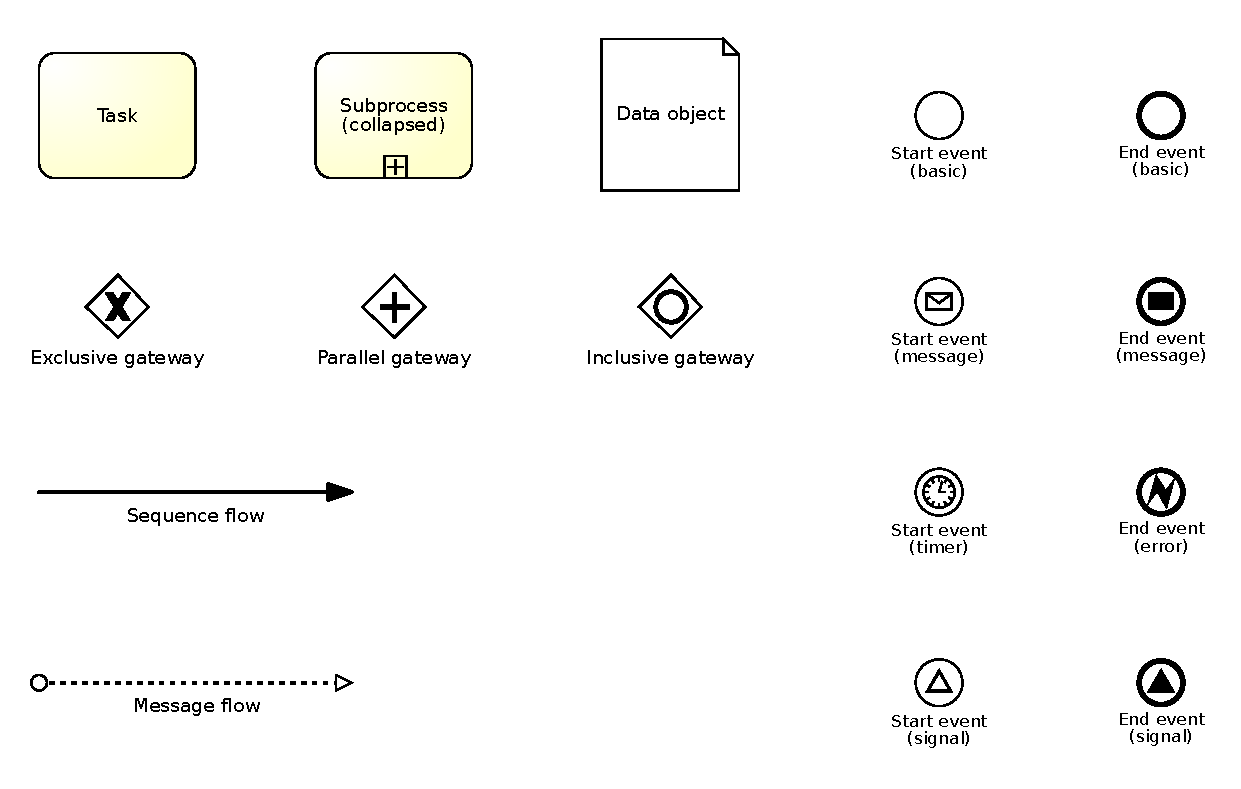
\includegraphics[width=\textwidth]{./images/bpmn_core_elements.pdf}
\caption{Graphical representation of basic BPMN elements}
\label{fig:bpmn_core_elements}
\end{figure}
Figure~\ref{fig:bpmn_core_elements} shows graphical representations of basic BPMN elements described above. Figure~\ref{fig:process_example} shows a simple example of a business process diagram. From the start event, the token is passed to the task ``Process the order''. Next task, ``Check out supplies status'' performs the data checkout, required for the exclusive gateway that appears next. When the commodity is available and the order can be completed, then the task "Accept the order" is carried out and whole process finishes. Otherwise, the process flow is split into two branches using parallel gateway. The two tasks performed next are ``Contact the supplier for restock'' and ``Inform the client about delay''. Next, the join parallel gateway synchronizes both paths and the process is finished.

\begin{figure}
	\centering
	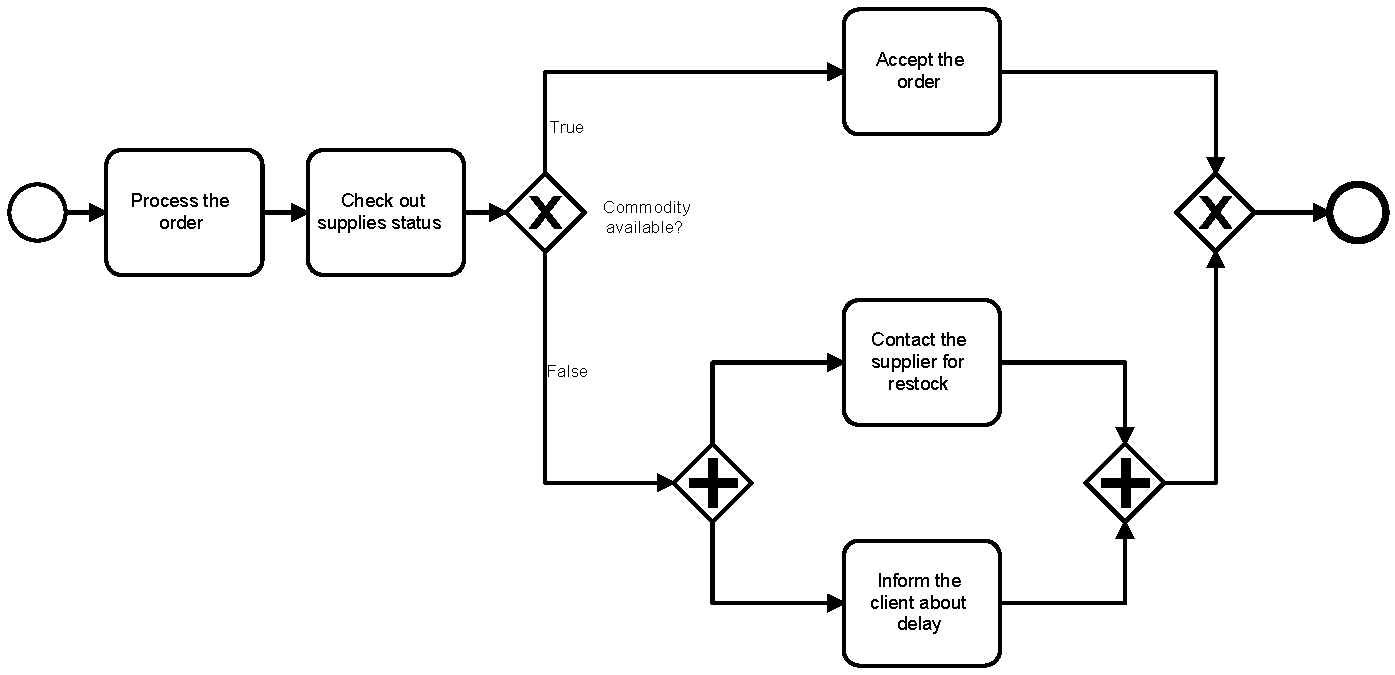
\includegraphics[width=\textwidth]{./images/process-example.pdf}
	\caption{An example of a simple BPMN business process}
	\label{fig:process_example}
\end{figure}

\section{Natural Language Processing}
\label{sec:nlp}
NLP~(\emph{Natural Language Processing}) is a branch of computer science, which combines elements of artificial intelligence and computational linguistics. NLP focuses on analysing and processing of natural language texts, in order to extract useful information and data, transforming them into an accessible for machines form. For the purpose of this thesis, two categories of NLP are important:
\begin{itemize}
	\item Syntax parsing -- grammatical analysis, parsing the syntax tree of the analysed text and part-of-speech (POS) tagging are the main concepts of this category,
	\item Semantic analysis -- extracting the meaning of words, which will be helpful in identifying the keywords, important from the business process point of view. 
\end{itemize}
There are many different tools which allows performing these tasks. A short description of both categories and the chosen tools will be given in the next subsections.

\subsection{Syntax parsing}
\label{subsec:syntax-parsing}
Syntax parsing focuses on determining the syntactic structure of a sentence (finding the grammatical relationships between words in analysed sentence) and part-of-speech tagging, which labels each word with a corresponding part of speech, based on its definition and context (i.e. adjacent words).\\
Examples of well-known tool used for the purpose of syntax parsing are NLTK (\emph{Natural Language Toolkit}), Stanford Parser or SpaCy parser project. For the purpose of syntax parsing, the SpaCy parser was chosen. SpaCy provides not only syntax parsing and POS tagging functionalities but is also able to perform tokenization, sentence decomposition, which will be useful for the purpose of this thesis.\\
The POS tagger provided by SpaCy utilizes two sets of Part-Of-Speech tags.  First one is based the OntoNotes 5 treebank~\cite{OntoNotes5},~\cite{ontnotes-2006}, which is based on earlier work, known as Penn Treebank~\cite{penntreebank-1993}. The secondary POS tag uses Universal Dependencies POS tags, which is simpler than the OntoNotes tags (for example there is only one tag for verbs -- OntoNotes provides tags for different tenses or persons).  Another important functionality of SpaCy is dependency parsing, which describes dependencies between words included in given sentence. Dependency parser used in SpaCy is based on ClearNLP project~\cite{ClearNLP}, with some extensions to dependency tags set. Figure~\ref{fig:sentence_example} shows an example of syntax tree, with Part-Of-Speech tag (from the OntoNotes tag set) and dependency tags, parsed from simple sentence ``This is an example of sentence, which can be parsed by SpaCy''.

\begin{figure}[ht]
	\centering
	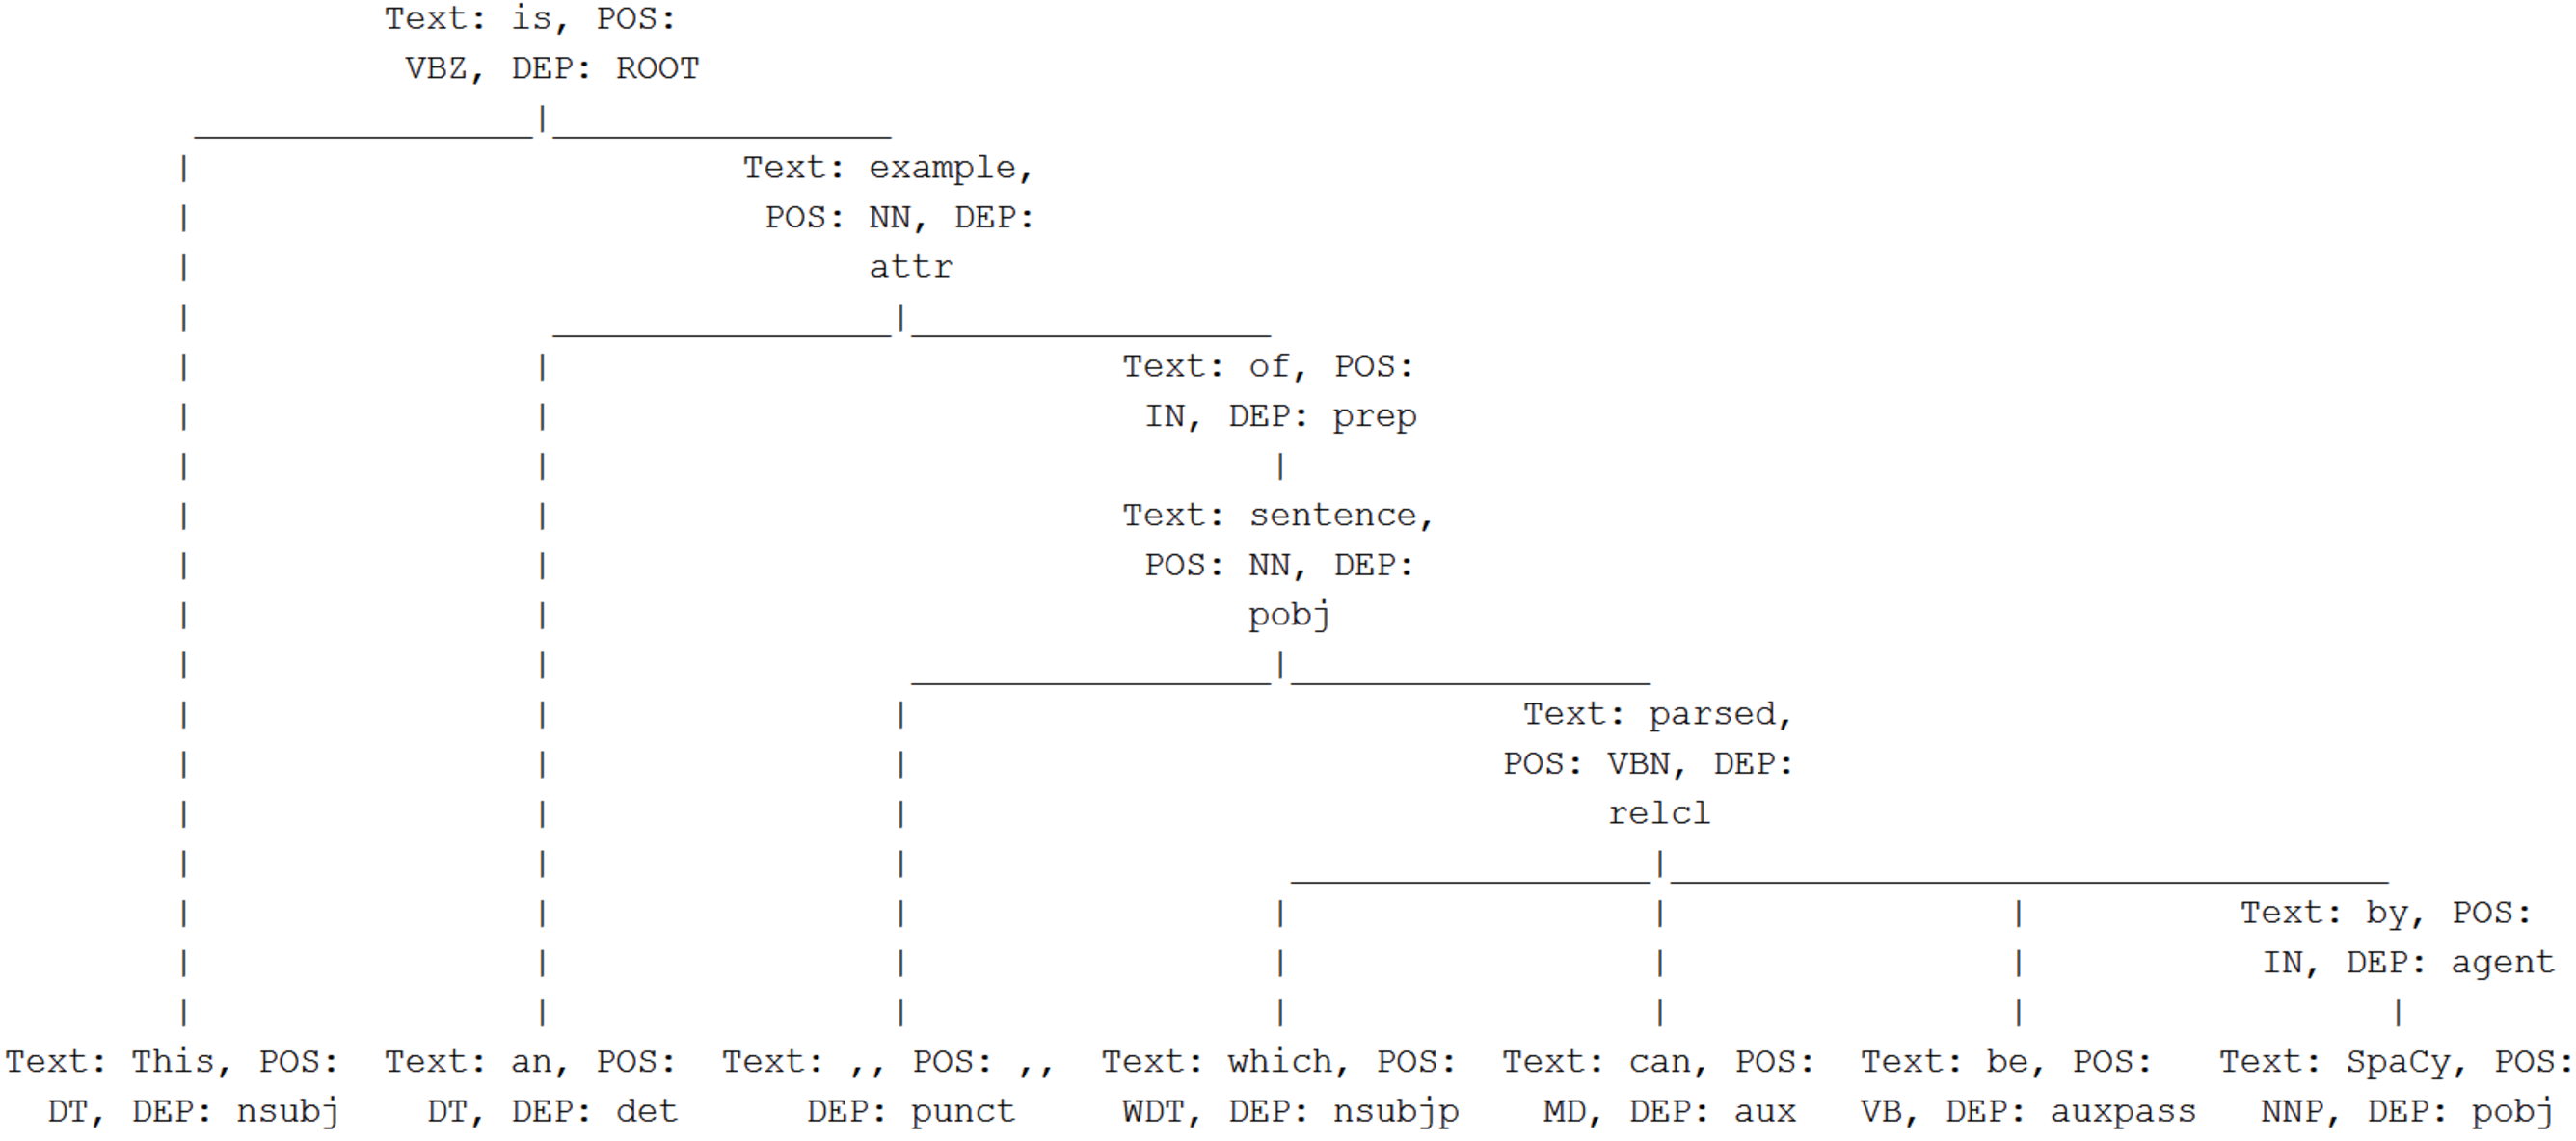
\includegraphics[width=\textwidth]{./images/sentence_example.pdf}
	\caption{An example of a sentence parsed by SpaCy}
	\label{fig:sentence_example}
\end{figure}

The dependency tag represents relation between child and parent in the tree. Notice that the word at the top of tree is tagged as ROOT.\\
Dependencies analysis is very helpful in determining the useful parts of natural language description, which can be later translated to BPMN process elements (mainly turning subject-verb-objects constructs into tasks). The full list of dependency tags available in SpaCy is described in Appendix~\ref{cha:dependencies-list}. Dependencies, which are used in proposed approach of translation, are shown in Table~\ref{table:dependencies}. This subset of dependencies should provide enough information to extract SVO (subject-verb-object) construct, which can be possibly translated into BPMN tasks. Auxiliary (\emph{aux}, \emph{auxpass}), modifier (\emph{amod}, \emph{neg}, \emph{prep}, \emph{poss}) and determiner dependencies can be used to extract additional words to better describe the extracted SVO.
\begin{table}[ht]
	\begin{tabular}{|l|c|}
		\hline
		Tag name & Description\\
		\hline
		\hline
		nsubj & nominal subject\\
		\hline
		nsubjpass & nominal passive subject\\
		\hline
		agent & agent\\
		\hline
		dobj & direct object\\
		\hline
		pobj & object of a preposition\\
		\hline
		iobj & indirect object\\
		\hline
		attr & attribute\\
		\hline
		conj & conjunct\\
		\hline
		compound & compound nouns or numbers\\
		\hline
		amod & adjectival modifier\\
		\hline
		aux & auxiliary\\
		\hline
		auxpass & auxiliary passive\\
		\hline
		neg & negation modifier\\
		\hline
		prep & prepositional modifier\\
		\hline
		poss & possession modifier\\
		\hline
	\end{tabular}	
	\caption{The subset of dependencies with definitions used in implemented prototype}
	\label{table:dependencies}
\end{table}
\subsection{Semantic analysis}
\label{subsec:semantic-analysis}
Semantic analysis focuses on interpreting the meaning of words in sentence. In the case of this thesis subject, semantic analysis allows us to eliminate information which was discovered during syntax analysis but is not useful from the business process point of view. As an example of such information, let us consider the sentences ,,Employee registers purchase'' and ,,Purchase is registered''. From the syntactic perspective, both of them should be treated as a subject-verb-object construct. Transforming them into BPMN tasks might be a correct decision -- in case of models made by business experts, it mostly depends on their point of view. Additional data, which can be extracted from these sentences, are information about people or inanimate entities (organizations, machines) involved in this task, which we will name as participants. In order to extract information about participants, we can validate if a given subject is synonymous to some general concept (for example ,,person'') which we assume to be a valid participant. In this case, ,,employee'' should be extracted as participant, but ,,purchase'' should be not.\\
Another use of semantic analysis is discovering some specific constructs, which indicate that some of the tasks are performed conditionally, excludes some other action or that a group of tasks can be executed simultaneously. This part of business process extraction will be explained further in section~\ref{cha:implementation}, which describes the algorithms in detail.\\
One of the most popular tools for semantic analysis is WordNet~\cite{word-net} -- a lexical database, which has been developed since 1985. WordNet contains information about sets of synonyms (synsets) for nouns, verbs, adjectives or adverbs. Different synsets are connected with each other by conceptual or lexical relations. Using WordNet, it is possible to analyse different semantic relations, such as synonyms, homonyms, hypernyms and other. This way, it should be possible to perform aforementioned analysis of extracted subjects and eliminate these that are not synonymous to some general concepts of participants.\\
Another useful functionality of WordNet is word stemming -- extracting the base meaning of word, removing lexemes. With the use of word stemming, it should be possible to produce normalized business process diagram and improve its readability and automatically create a unified tasks naming convention.

\section{Related work}
\label{sec:related}
In their recent publication~\cite{process-mining-state-of-the-art}, Terins and Thaler performed an analysis of current state-of-the-art in the field of mining process models from natural language text. A several different approaches were presented, some of which worked with some form of structuralized text (use cases, group stories), some with natural language description.
\begin{itemize}
\item Ghose, Koliadis and Chueng~\cite{proces-from-text-artefacts} proposed an approach for discovering a process model from text artefacts, which are described as \emph{documents such as memos, manuals, requirements documents, design documents, mission/vision statements, meeting minutes etc.} An extraction is performed by text pattern search (for example if/then pair, which indicates a conditional flow) and POS (\emph{Part-Of-Speech}) tagging combined with shallow parsing, which produces a syntax tree. This approach allows to discover parts of a larger model (called \emph{proto-models} by authors), rather than complete and sound model. Generated \emph{proto-models} can be compared in order to find similarities and remove redundant parts.

\item Goncalves et al.~\cite{mining-group-stories} presented a technique of obtaining process models from group stories. In the first phase, a text is tokenized in order to select words which can be useful for work-flow generation. Next, a POS tagging is performed. Finally, relevant entities are identified using a set of predefined patterns.
The produced BPMN model is not necessarily complete and sound -- it is assumed, that it will be later improved by process designer and team members, who created the group stories.
\begin{figure}[h!b]
	\centering
	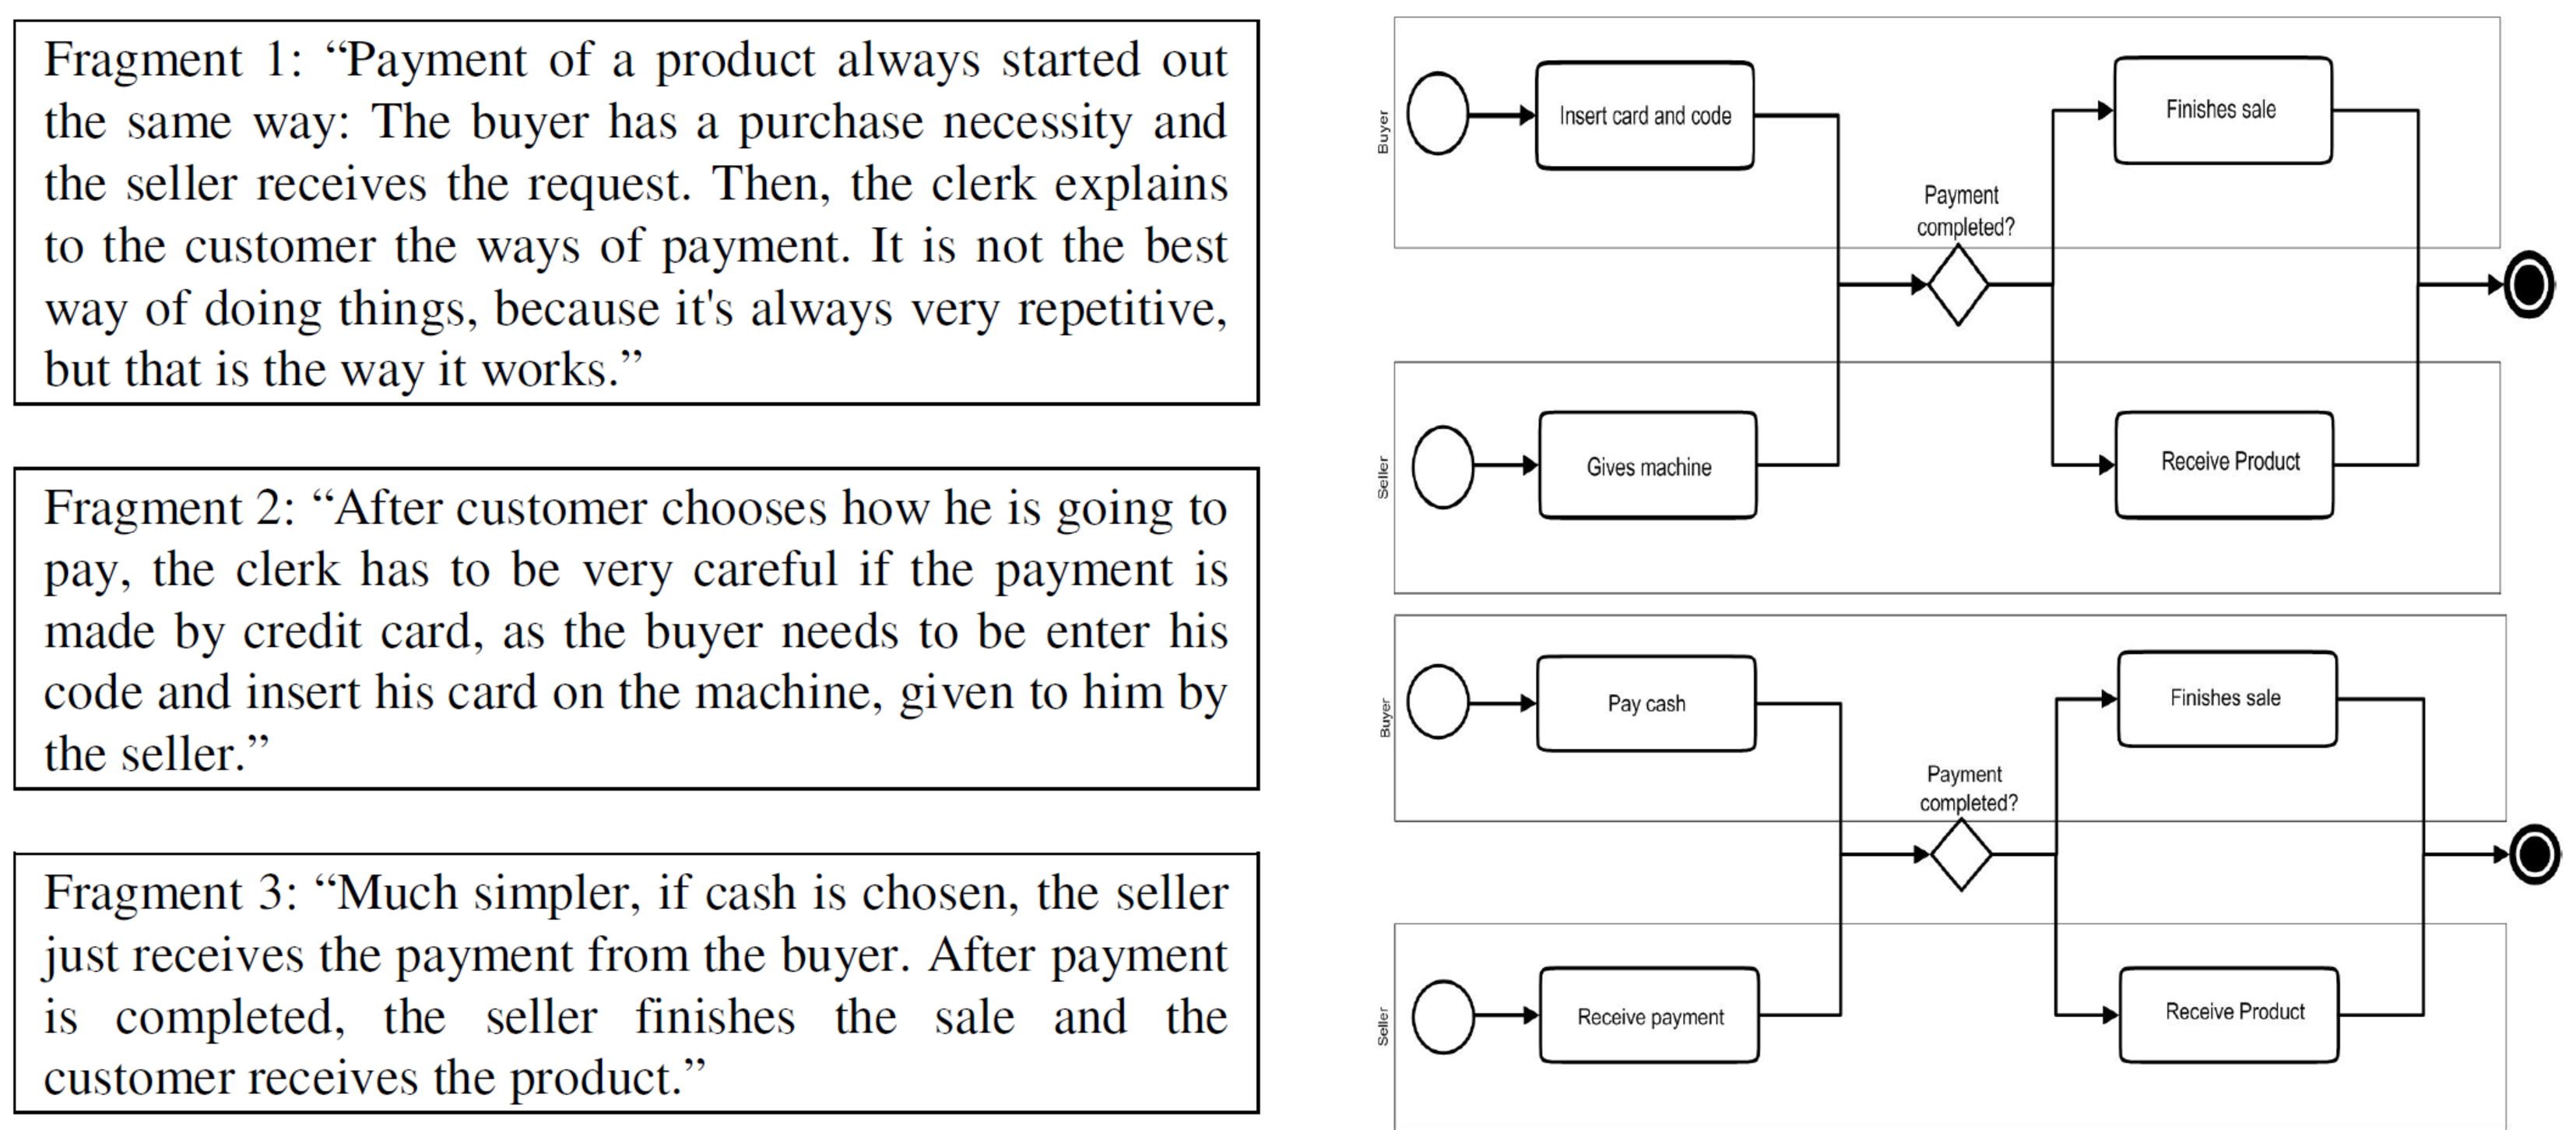
\includegraphics[width=\textwidth]{./images/goncalves_transform.pdf}
	\caption{Fragments of group story with corresponding BPMN elements generated by algorithm described in paper~\cite{mining-group-stories} (example obtained from article)}
	\label{fig:goncalves_example}
\end{figure}

\item Friedrich et al.~\cite{friedrich-2011} proposed an advanced approach, which uses a textual description of model. Such a description must follow some requirements -- a text cannot contain any questions and the described execution of a process must be sequential (any non-sequential jumps must be explicitly made). In the first step, a syntactical analysis (called \emph{Sentence Level Analysis} in the article) is performed, using Stanford NLP tools. Next, the semantic analysis (\emph{Text Level Analysis}), using WordNet and FrameNet databases, allows to identify relevant entities. Finally, the process model is generated (\emph{Process Model Generation} phase). Detailed flows for each phase are shown in Figures~\ref{fig:friedrich_sentence_analysis}~\ref{fig:friedrich_text_analysis}~\ref{fig:friedrich_process_generation}. The generated output is a sound and complete BPMN model, enriched with many additional elements (such as lanes, data sources), thanks to the rich text analysis. 
\end{itemize}
Several other methodologies for transforming natural language text into formalised models were proposed. Yue, Briand and Labiche~\cite{yue-2010} presented an automated approach to transform use case descriptions to UML Activity diagrams. This methodology requires that the use case descriptions has to follow some restriction rules. These rules can be classified into two groups -- the first group specifies constraints on the use of natural language, the second are requirement on the use of specific keywords to indicate the existence of control structures. In addition, the use case description explicitly lists all of the flows in the process (main and alternative) and each flow is a step-by-step description of a process.\\
Another approach in the field of generating formal models form natural language specification, proposed by Njonko and Abed~\cite{from-nl-to-model-via-sbvr}, uses SBVR (\emph{Semantics or Business Rules and Vocabulary}) as an intermediate layer for this transformation approach. It is suggested that using formalised model as an intermediate layer (in this case SBVR), it is possible to easily extend this approach for multiple models. The article presents an example of transformation from natural language business description into SQL executable query, which produces a database table that corresponds to business requirements.\\
In this section, the basic information about Business Process Management, BPMN notation and NLP was presented. Also, the SpaCy parser and the underlying technology of this tool were described. Next section describes the proposed approach to the problem and the implementation of prototype, which is based on SpaCy parser and utilizes the described NLP methods.
\begin{figure}[H]
	\centering
	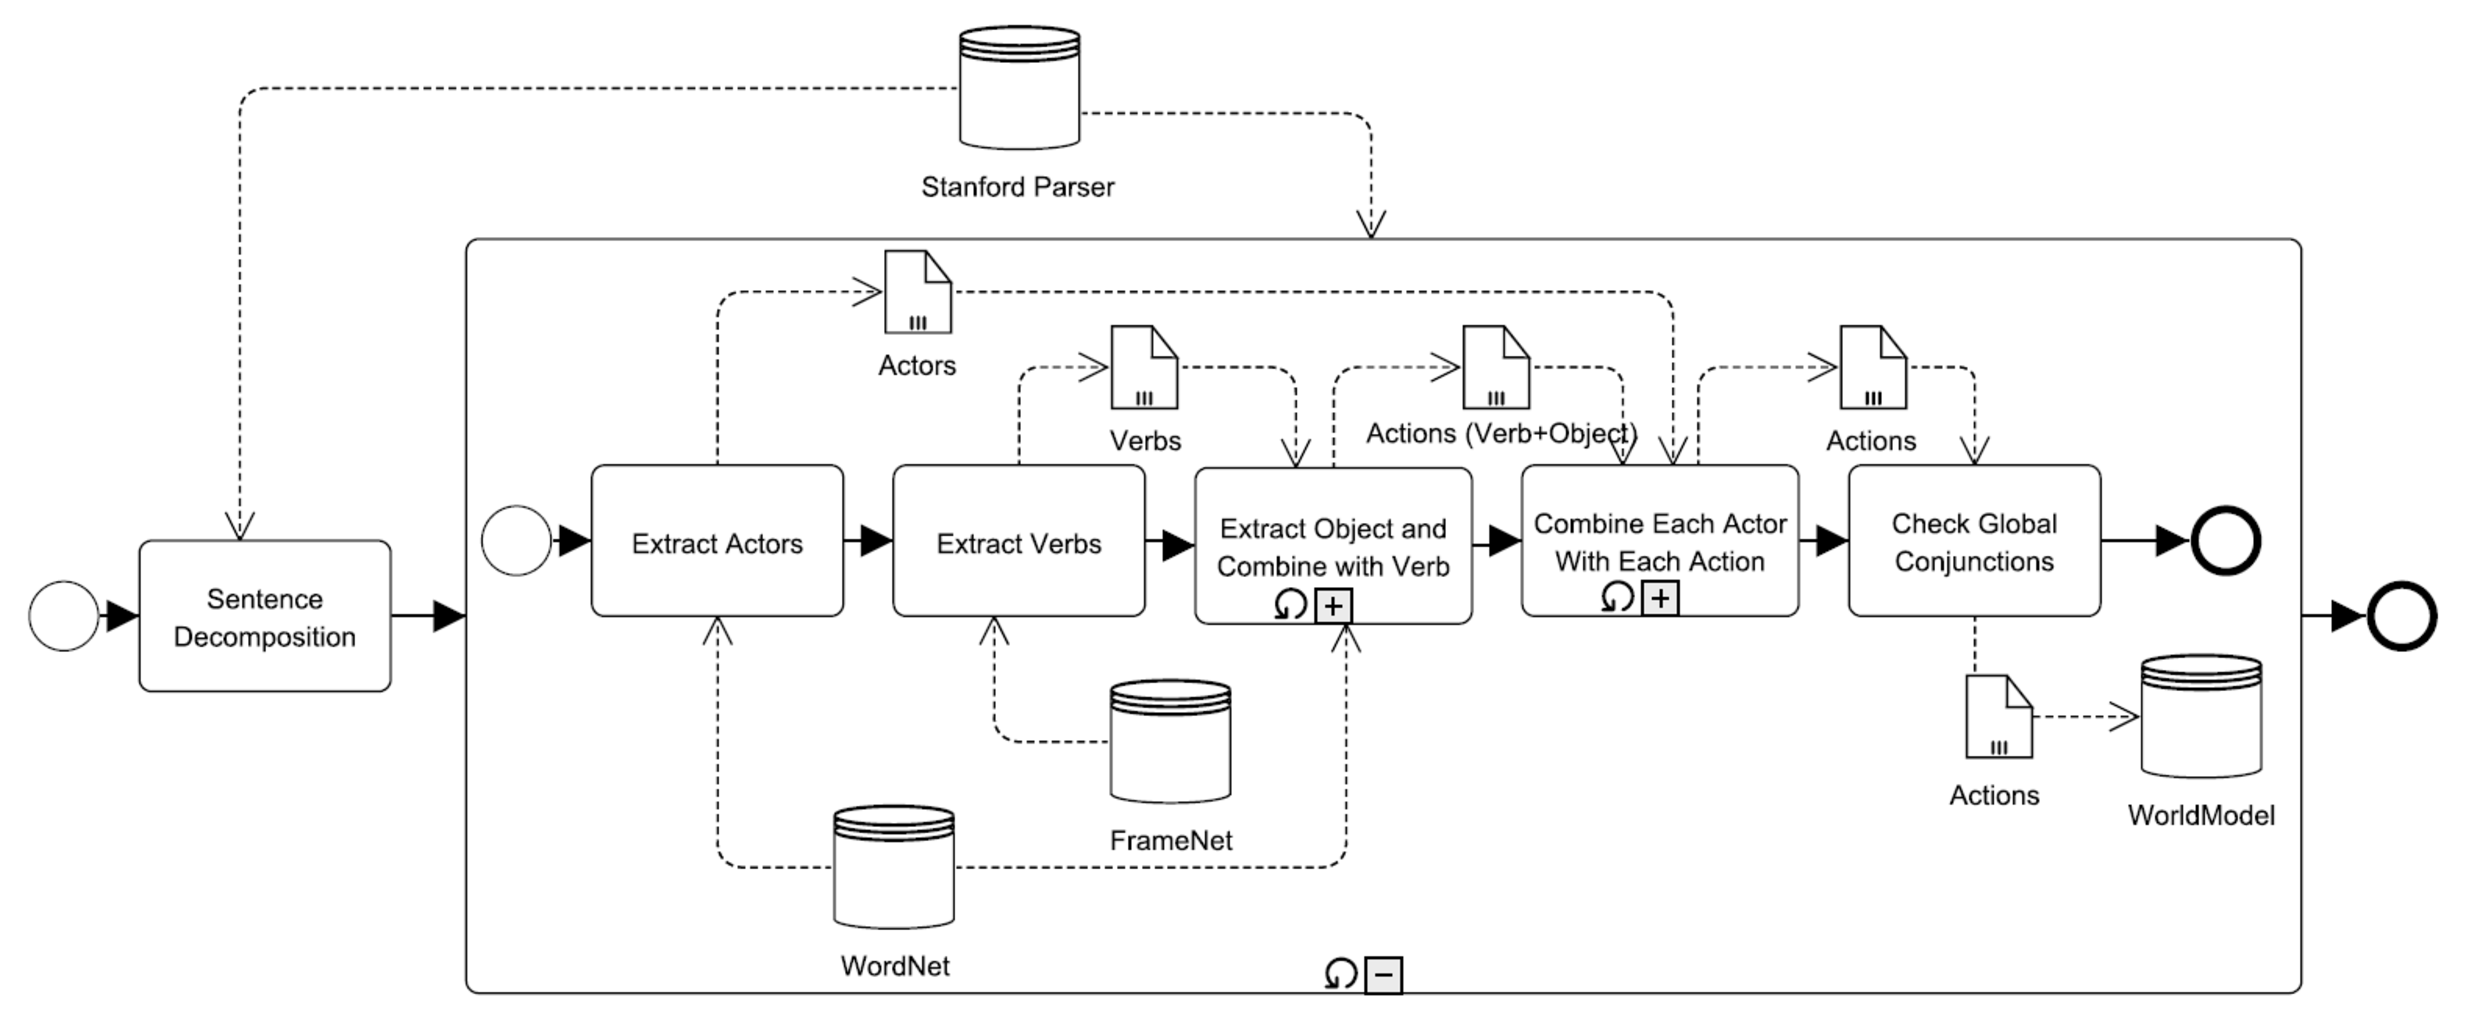
\includegraphics[width=\textwidth]{./images/friedrich_sentence_analysis.pdf}
	\caption{Detailed flow showing sentence analysis phase of transformation approach described in article~\cite{friedrich-2011} (diagram obtained from article)}
	\label{fig:friedrich_sentence_analysis}
\end{figure}
\begin{figure}[H]
	\centering
	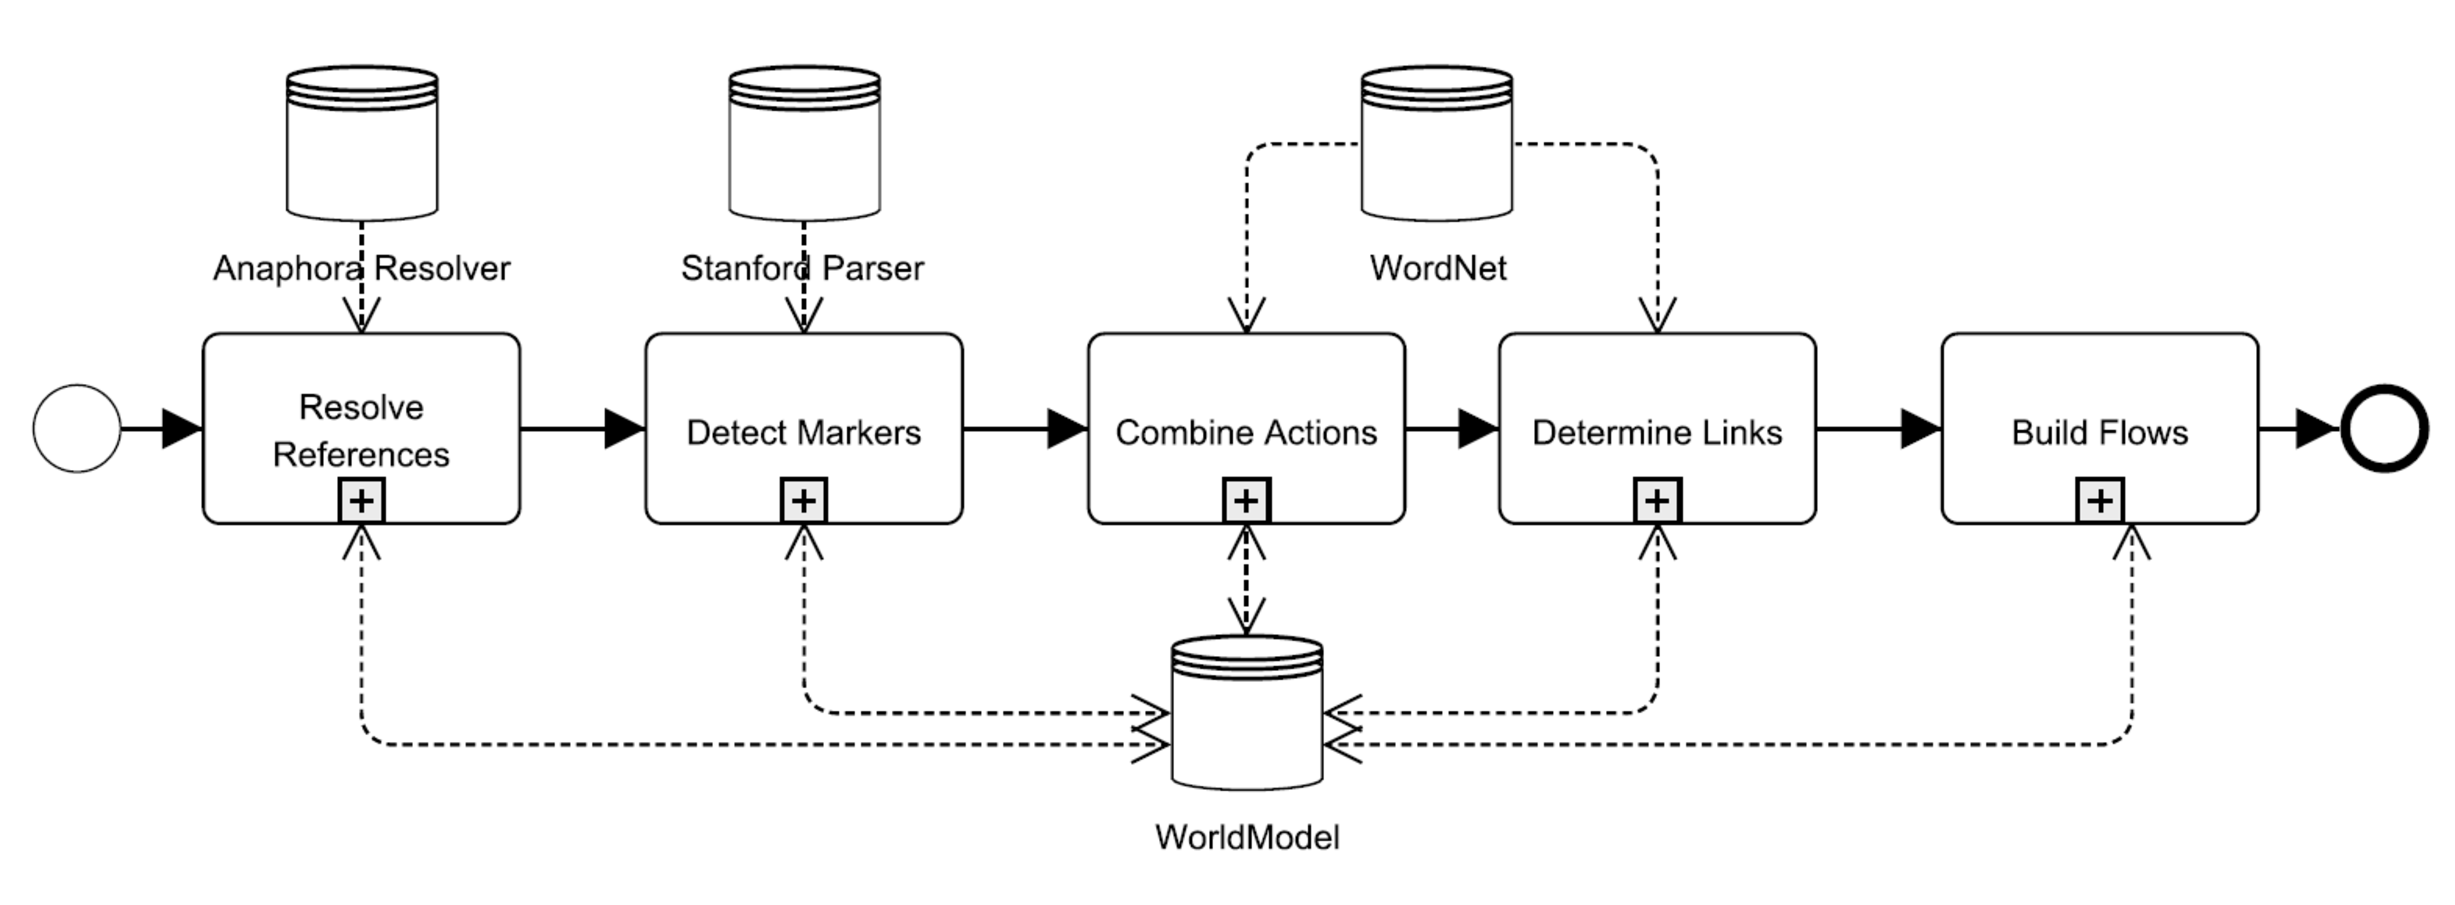
\includegraphics[width=\textwidth]{./images/friedrich_text_analysis.pdf}
	\caption{Detailed flow showing text analysis phase of transformation approach described in article~\cite{friedrich-2011} (diagram obtained from article)}
	\label{fig:friedrich_text_analysis}
\end{figure}
\begin{figure}[H]
	\centering
	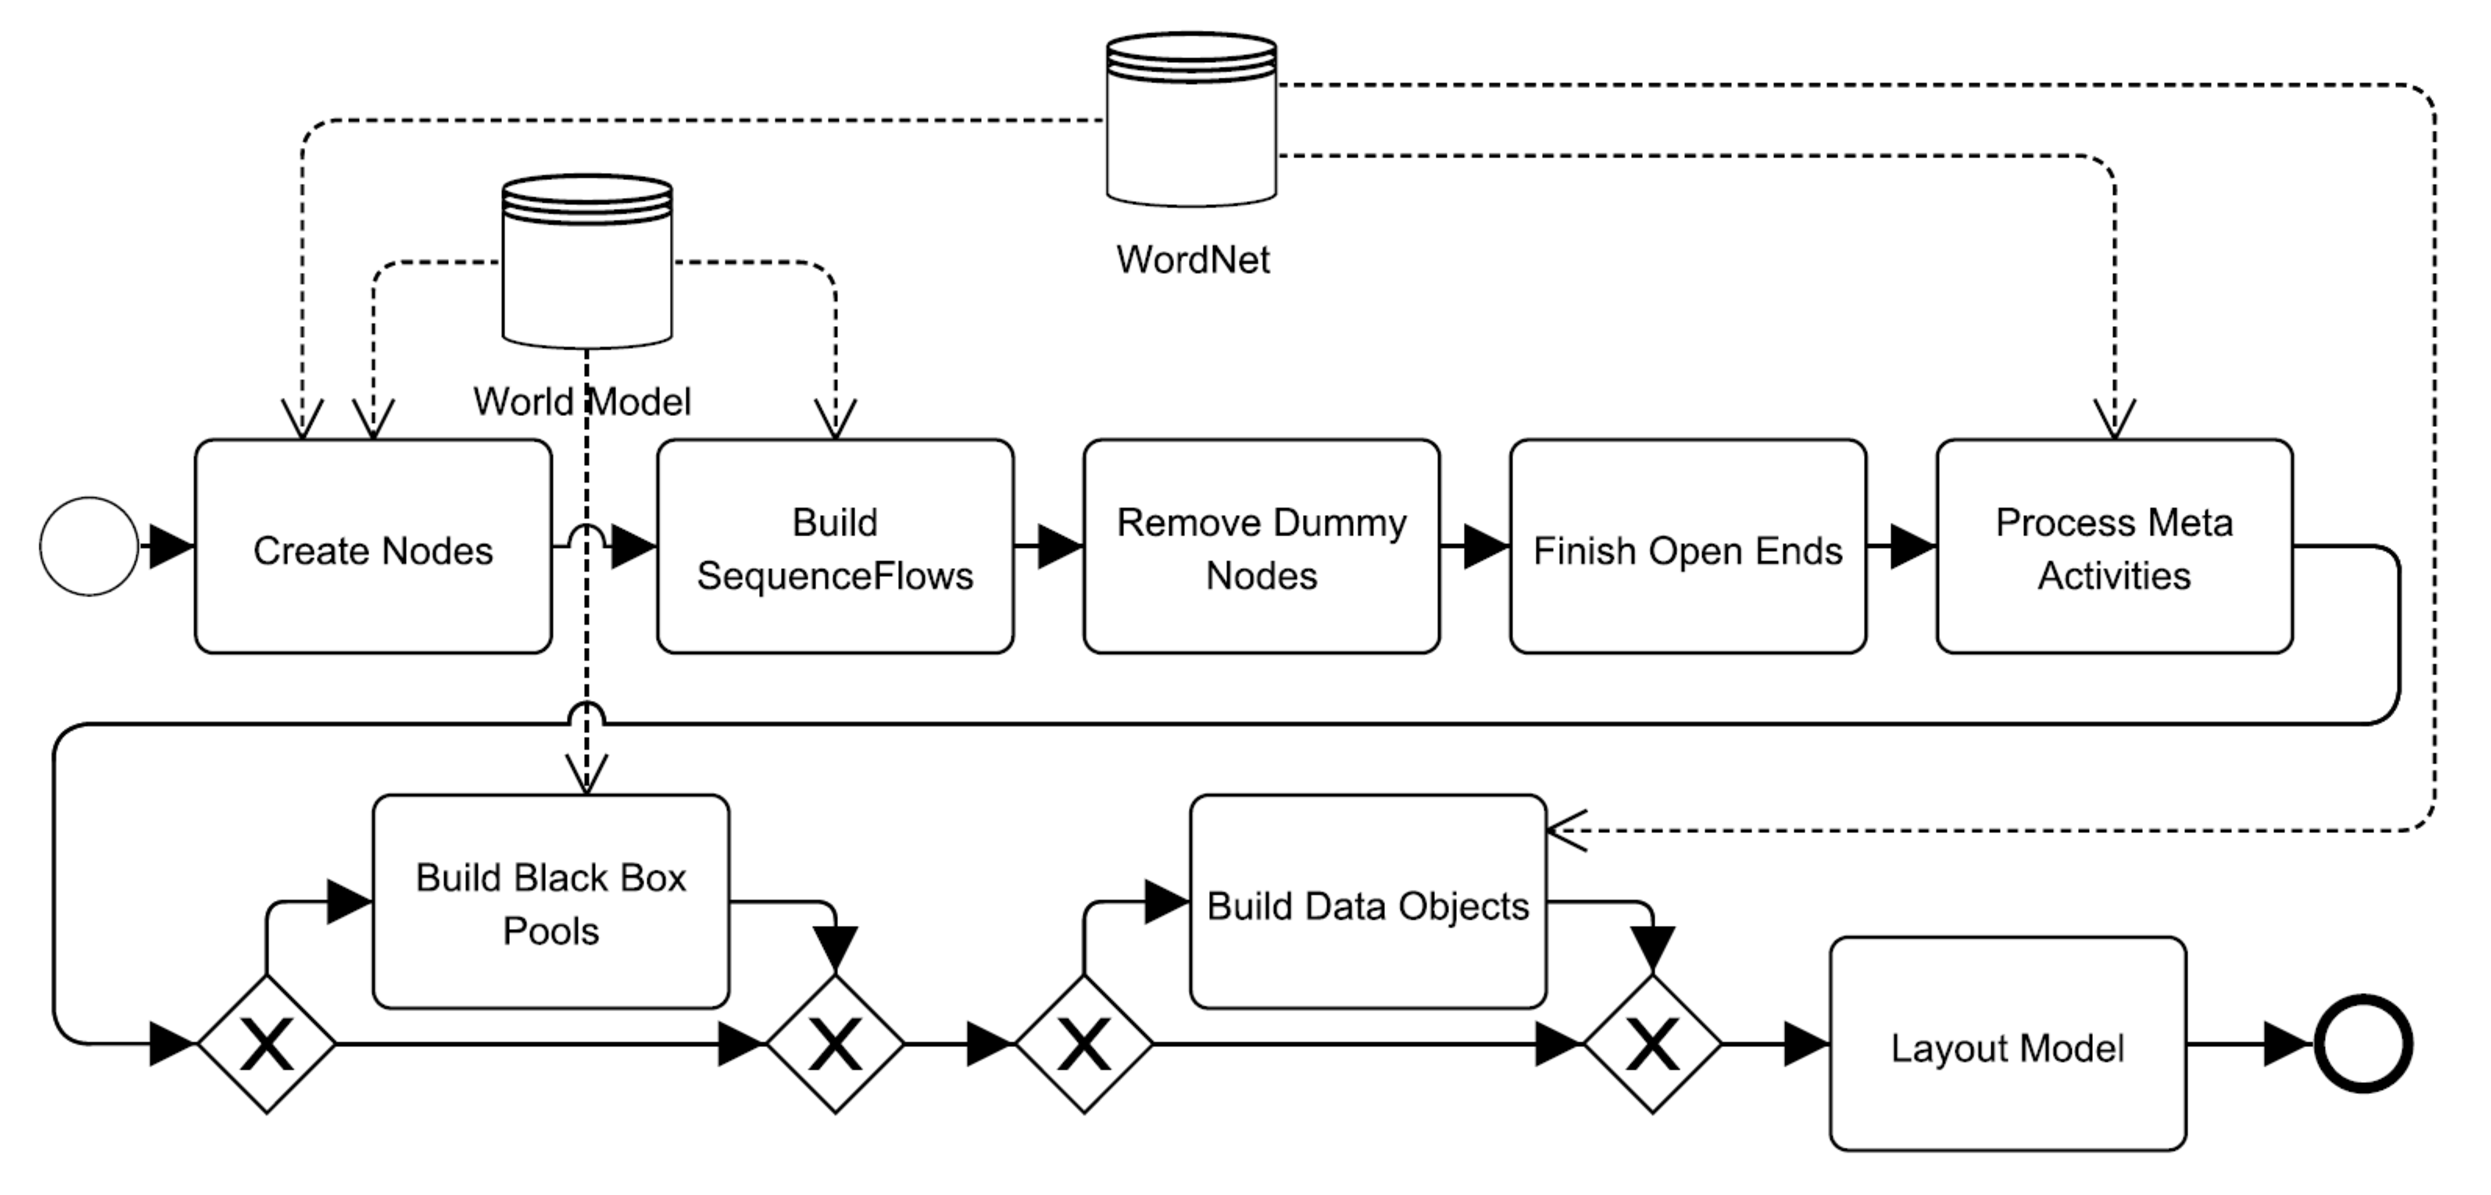
\includegraphics[width=\textwidth]{./images/friedrich_process_generation.pdf}
	\caption{Detailed flow showing process generation phase of transformation approach described in article~\cite{friedrich-2011} (diagram obtained from article)}
	\label{fig:friedrich_process_generation}
\end{figure}
\begin{figure}[H]
	\centering
	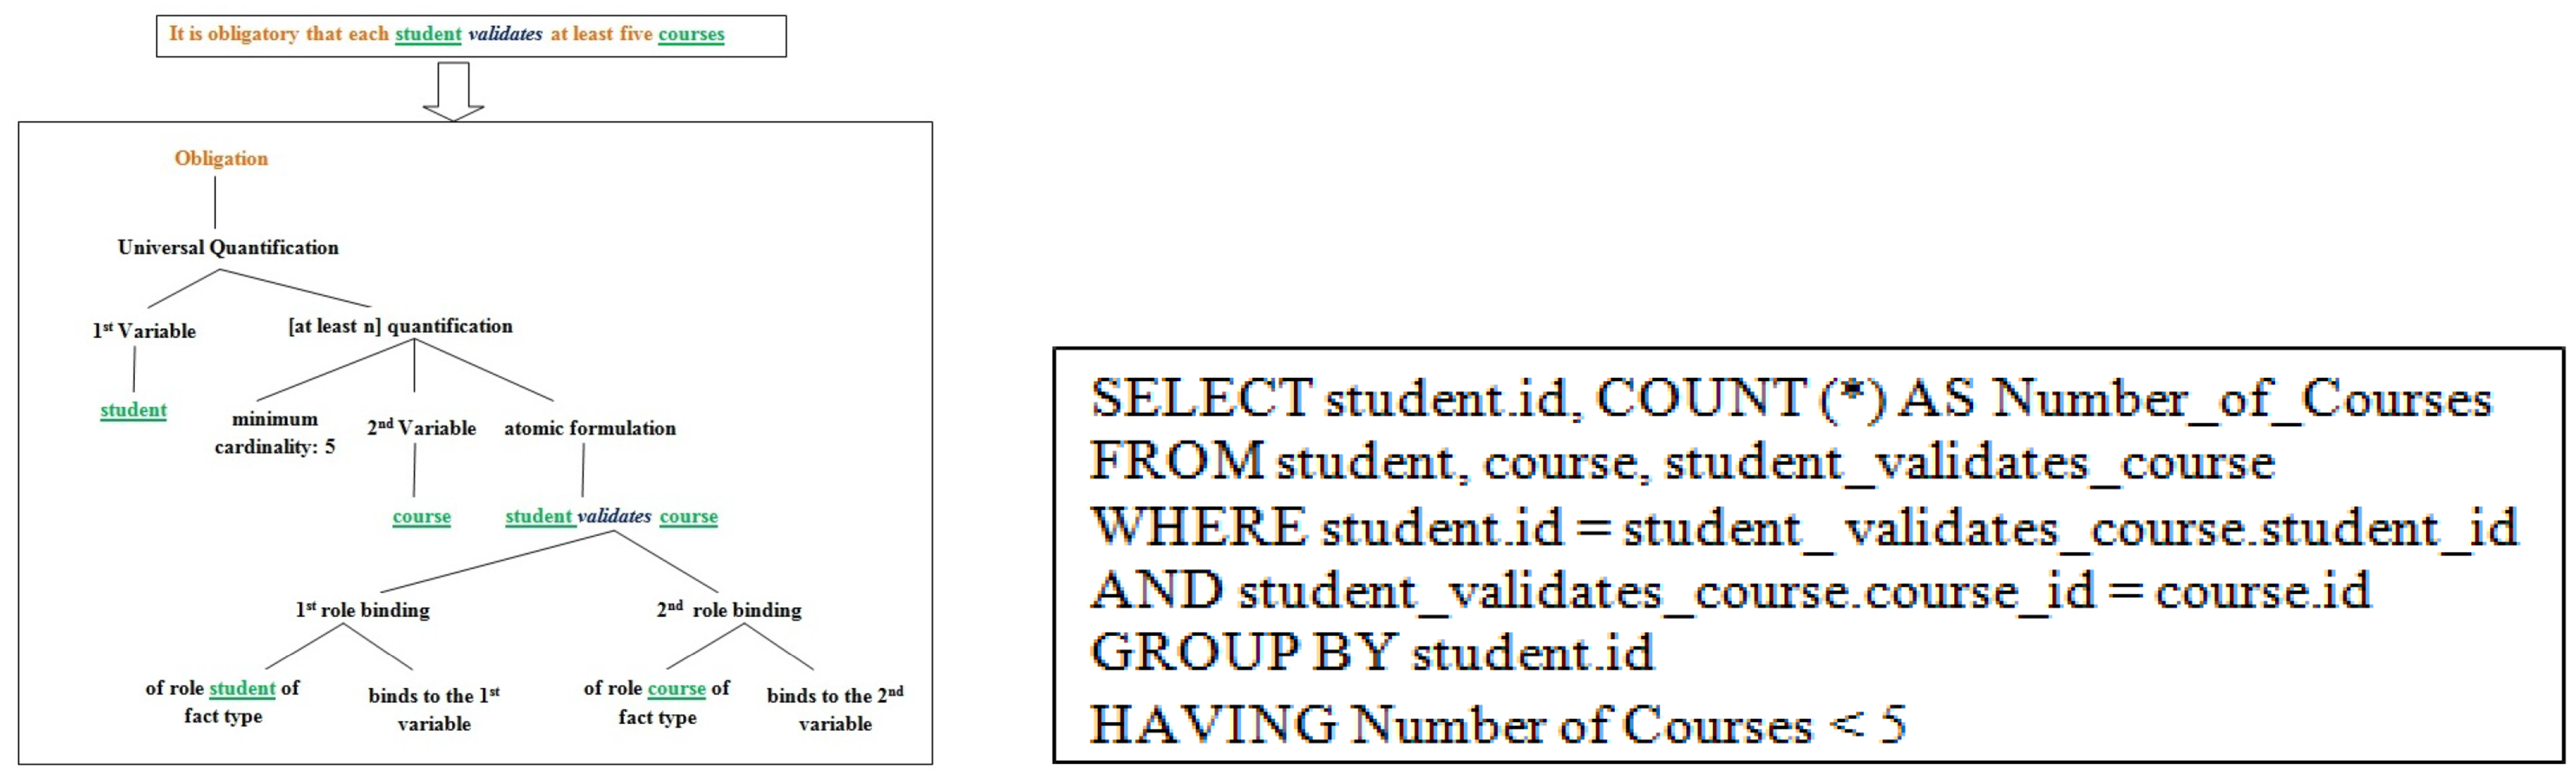
\includegraphics[width=\textwidth]{./images/njonko-example.pdf}
	\caption{An example of SQL query generated from business description, using method described in article~\cite{from-nl-to-model-via-sbvr} (pictures obtained from article)}
	\label{fig:njonko_example}
\end{figure}
\chapter{Implementation}
\label{cha:implementation}
This section describes the proposed approach to business process model generation from natural language description. This approach can be divided into the following steps:
\begin{enumerate}
	\item Participants extraction -- in this step, a sentence from a given description is analysed and the information about possible participants (people, systems or organizations which performs the tasks) in process are extracted,
	\item Subject-verb-object constructs extraction -- a sentence from given description is analysed in search of basic SVO constructs, which later will be used to create appropriate BPMN elements,
	\item Gateway keywords search -- a process description is analysed in search of the keywords that signalizes the presence of conditional (exclusive or inclusive) and parallel gateways,
	\item Intermediate process model generation -- an intermediate process model is created from the acquired data,
	\item BPMN diagram generation -- a BPMN diagram is generated from the intermediate process model.
\end{enumerate}
Figure~\ref{fig:method_overview} shows the overview of proposed approach.\\
The generated intermediate model is parsed to BPMN diagram, using functionality provided by bpmn\_python library\footnote{\url{https://github.com/KrzyHonk/bpmn-python}, last access: \onlineAccess. \emph{bpmn\_python} was created as a part of other university project by Izabela Śmietana and Krzysztof Honkisz, with additional contributions from Krzysztof Płachno, Tomasz Gargas and Renata Gargas.}. The prototypical tool implemented for the purpose of this thesis generates both spreadsheet-based intermediate model and BPMN diagram, which makes the result analysis easier.
\begin{figure}[H]
	\centering
	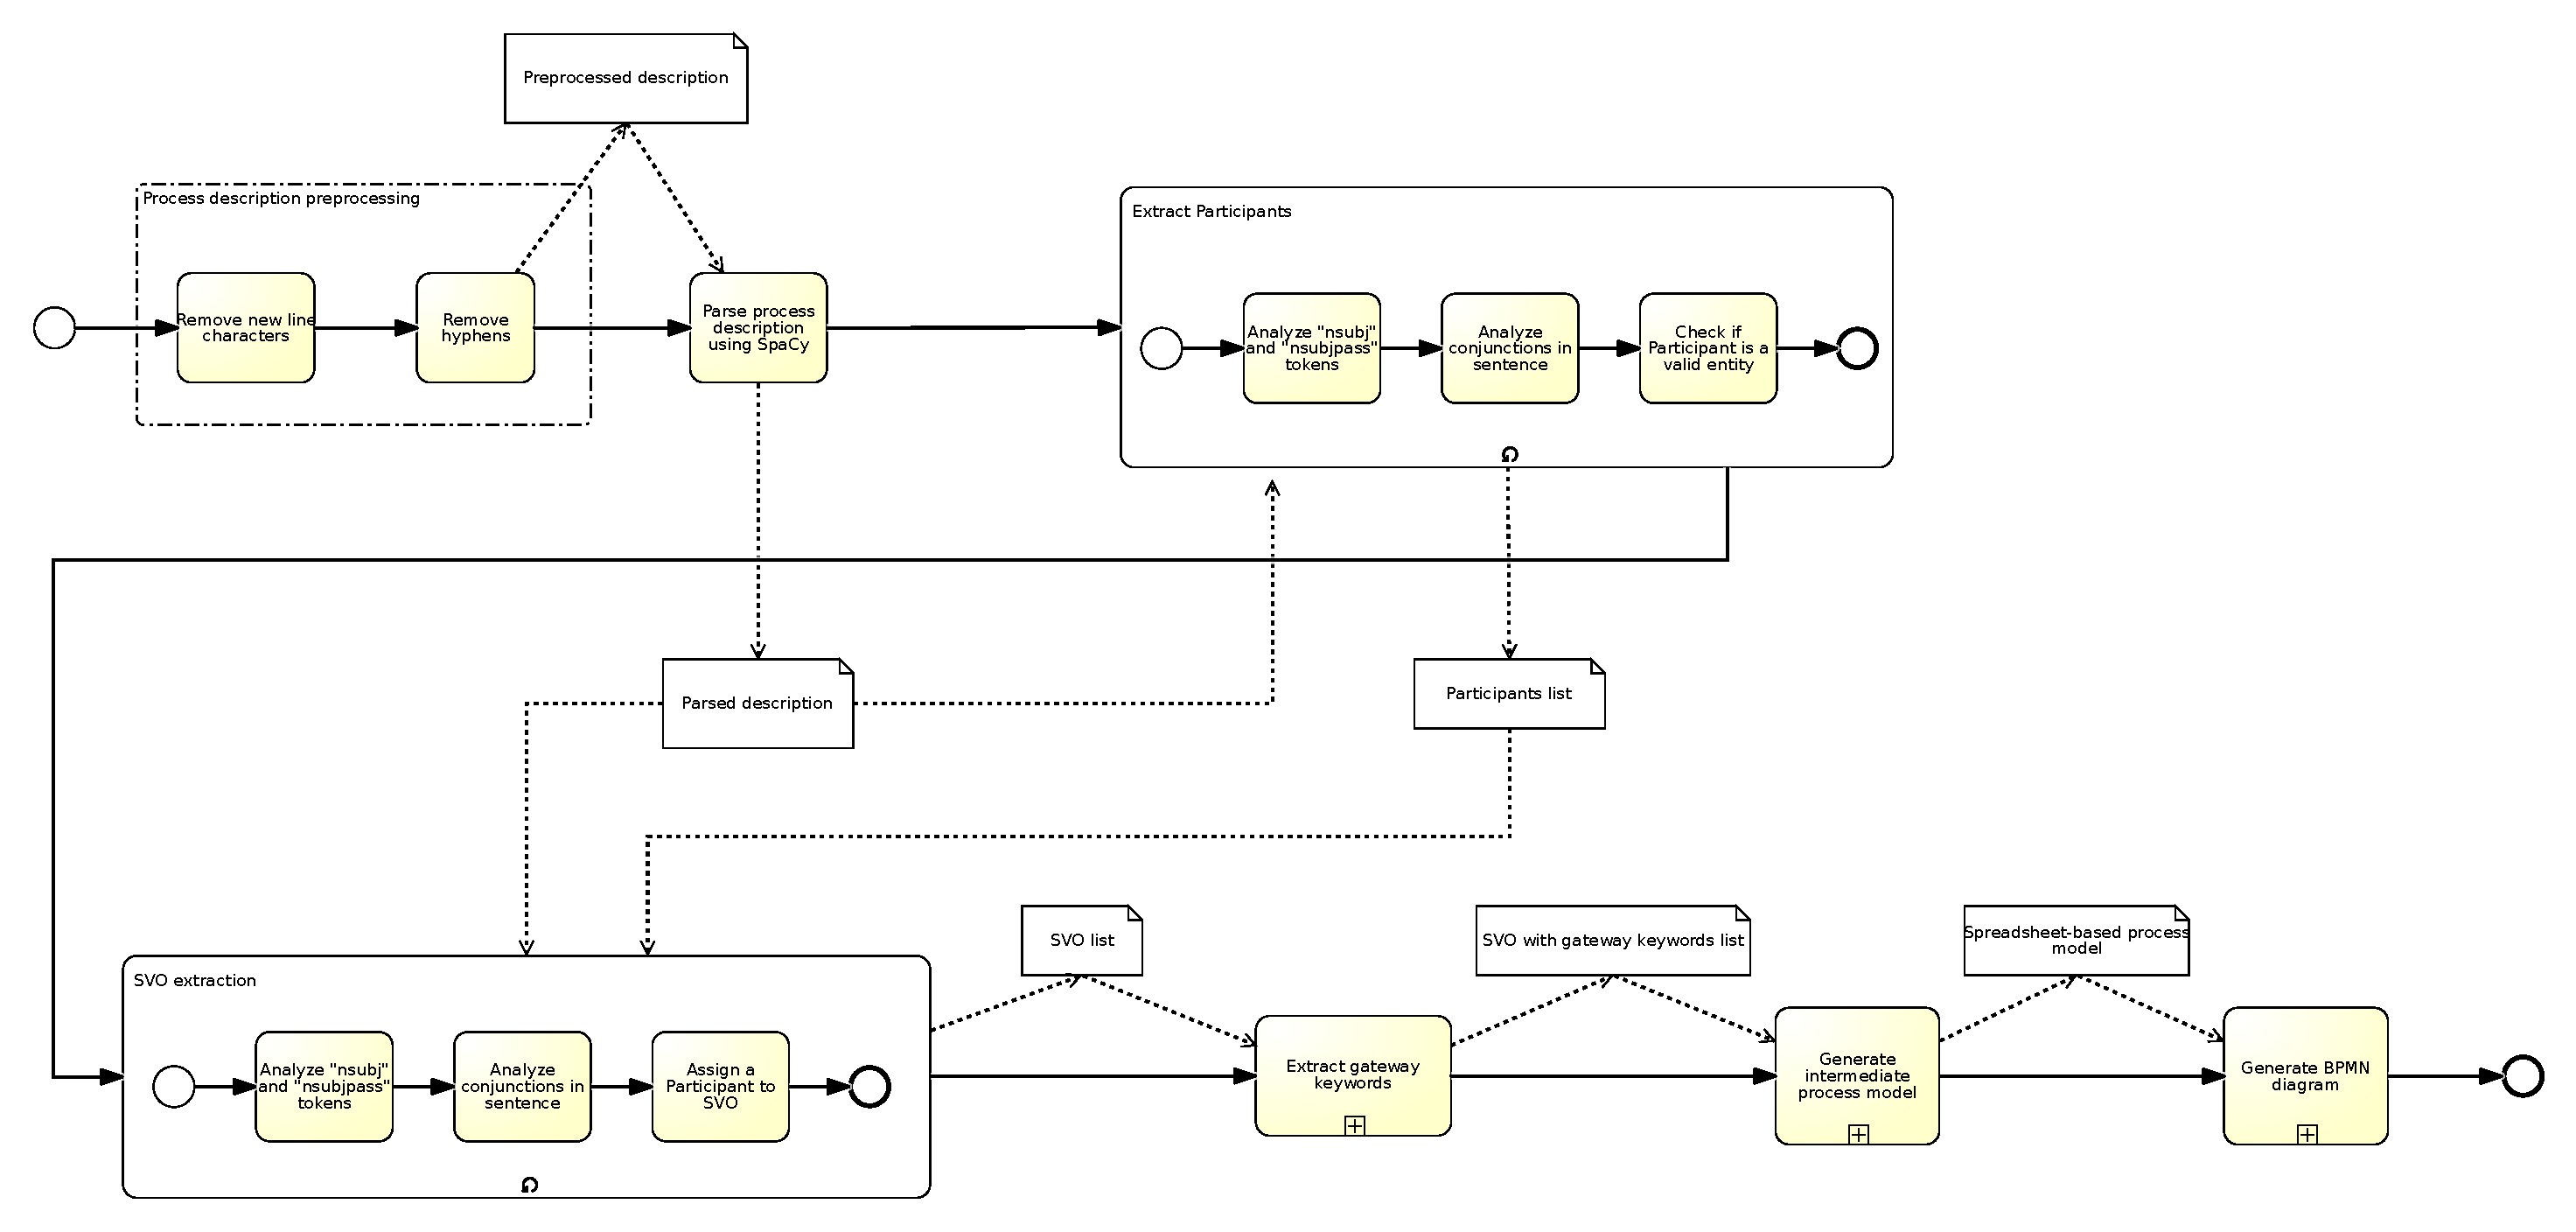
\includegraphics[width=0.95\textheight, angle=90]{./images/method_overview.pdf}
	\caption{BPMN diagram with overview of proposed approach.}
	\label{fig:method_overview}
\end{figure}

\section{Functional requirements}
The main functional requirement for the prototypical tool was portability of the created program. Thus, the prototype was implemented in Python language, since there are many implementations of Python interpreter, with official support for the most popular operating systems. In addition, many NLP processing tools (including SpaCy and WordNet) provide an API implemented in Python, thus Python is an interesting choice for many project from this field of computer science.\\
The tool was implemented using the newest, third version of Python language. This choice was made due to the fact, that third version provides a few new and interesting functionalities (such as built-in support for type annotation\footnote{\url{https://www.python.org/dev/peps/pep-0484/}, last access: \onlineAccess.}). Also, second version of Python language is officially considered as legacy version and no longer will be supported\footnote{\url{https://wiki.python.org/moin/Python2orPython3}, last access: \onlineAccess.}.\\
The prototypical tool works with SpaCy parser, version 1.6 -- this version was the newest one at the beginning of work.

\section{Participants extraction}
\label{sec:participant}
In the first step, each sentence of the description is analysed in search of words that represents participants in process. This process is divided into three parts.\\
First, the sentence is analysed in search of specific dependency relations, namely \emph{``nsub''} (nominal subject) and \emph{``nsubjpass''} (nominal subject passive). Whenever a token with one of these dependencies is found, it is added to the list of possible participants.\\
Next, the sentence is searched for conjunction (\emph{``conj''}) dependencies. In this case, the participant might be labelled as an object of the phrase. Therefore, the tokens belonging to the syntax sub-tree of conjunction is searched in order to find object-related dependency labels, that is \emph{``attr''} (attribute), \emph{``dobj''} (direct object), \emph{``iobj''} (indirect object) and \emph{``pobj''} (object of a preposition). For example, in the sentence: \emph{``It is given either by a sales representative or by a presales employee''} (syntax tree presented in Figure~\ref{fig:participant_conj_example}), the possible participant \emph{``employee''}, is labelled as object of preposition and word \emph{``by''} is labelled as a part of conjunction. Adding the conjunction check, it is possible to extract this information.\\
Figure~\ref{fig:participant_extraction_subprocess} shows BPMN diagram presenting overview of Particpant extraction algorithm.
\begin{figure}[H]
	\centering
	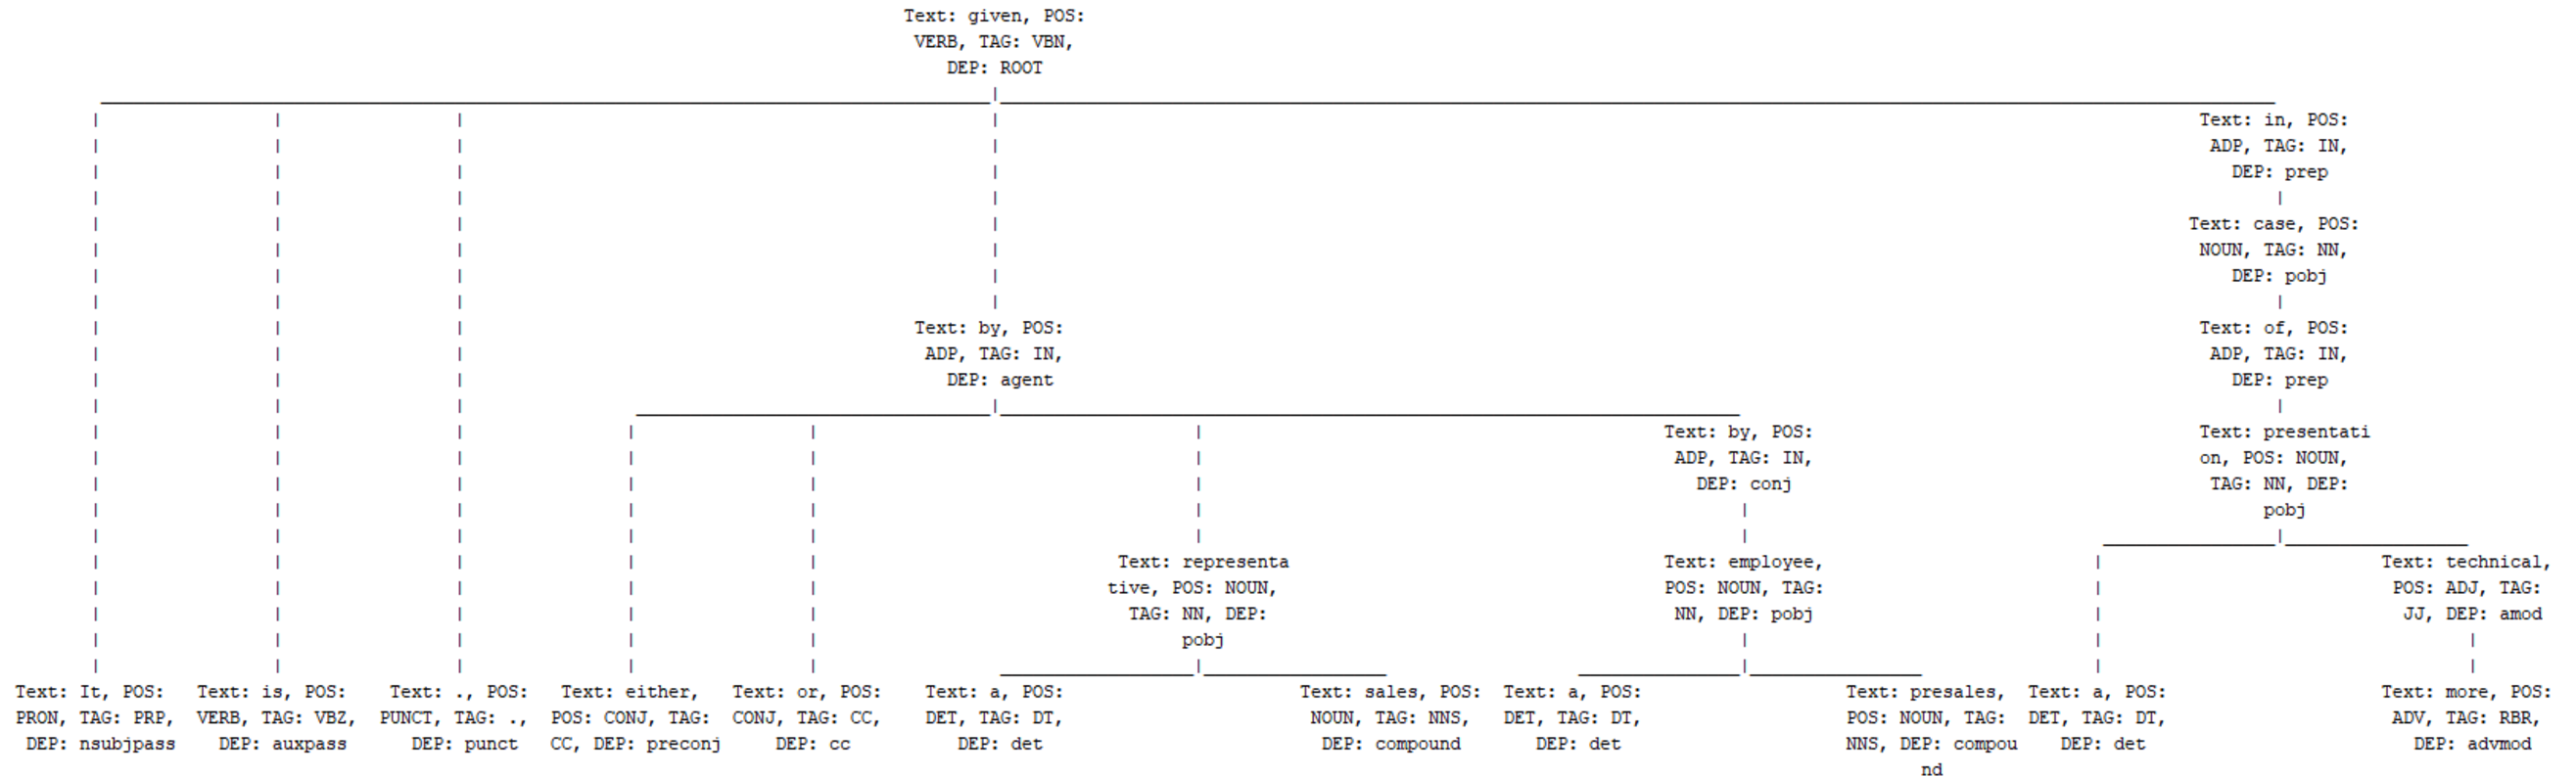
\includegraphics[width=\textwidth]{./images/participant_conj_example.pdf}
	\caption{Syntax tree for simple phrase \emph{``It is given either by a sales representative or by a presales employee in case of a more technical presentation.''} Word \emph{``employee''}, connected with conjunction dependency can be extracted as possible participant in business process.}
	\label{fig:participant_conj_example}
\end{figure}
\begin{figure}[H]
	\centering
	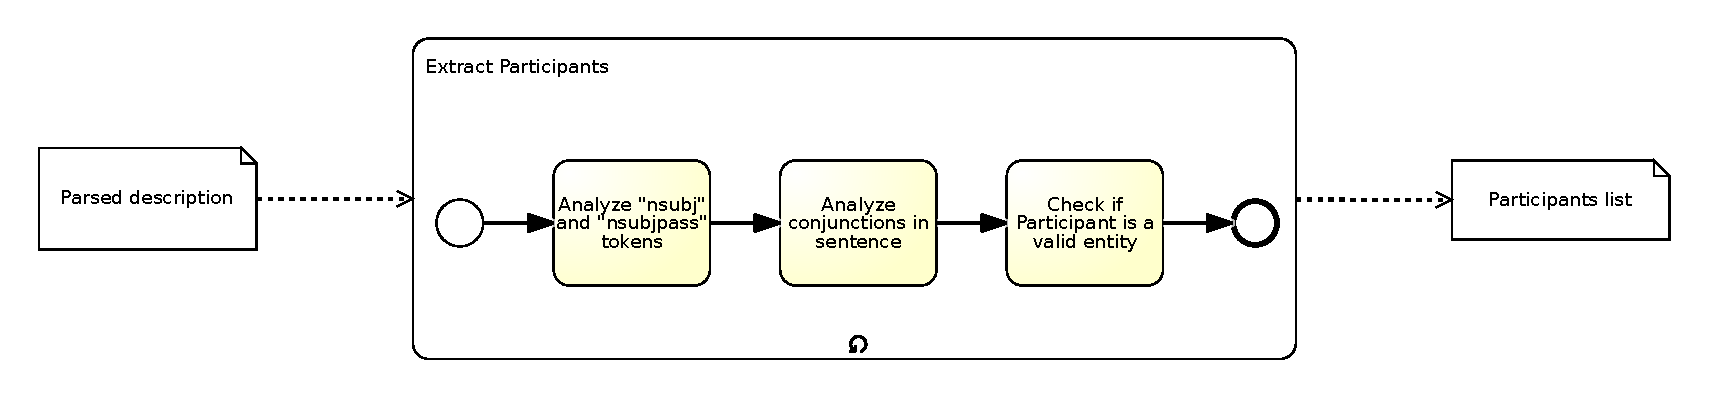
\includegraphics[width=\textwidth]{./images/participant_extraction_subprocess.pdf}
	\caption{BPMN diagram presenting overview of Particpant extraction algorithm}
	\label{fig:participant_extraction_subprocess}
\end{figure}
Every time, when a possible participant is added, its Part-Of-Speech tag -- based on Universal Dependencies tag set (mentioned in Section~\ref{subsec:syntax-parsing}) -- is checked. If the participant is tagged as a pronoun (\emph{pron}), a special flag is set for a given object.\\
Finally, a simple semantic analysis is used to decide, whether the extracted words can be used as participants of process. The extracted word is added to output as a participant if it fulfils one of these conditions:
\begin{itemize}
	\item the word is a pronoun or relative pronoun. In this case, the Participant is accepted as a valid entity,
	\item one of the hypernyms, derived from the analysed word, belongs to the specified list of hypernym keywords, accepted as participants. Examples of such keywords are \emph{``person''} or \emph{``organization''}. The full list of used hypernyms is shown in Table~\ref{table:participants-hypernyms}. Hypernyms of participant word are derived using WordNet lexical database,
	\item the word is equal to some special keyword. This case was added, because WordNet might not contain some specific words in the database, therefore hypernym analysis does not provide any proper result. An example could be the word CRM (Customer Relationship Management). A full list of keywords used in this prototype is shown in Table~\ref{table:participants-keywords}. List was composed through analysis of test set of process descriptions.
\end{itemize}	
Each of the Participants have a full name assigned, which is extracted from its syntax sub-tree, provided that a given token from sub-tree is labelled with a correct dependency. In case of Participant, the following dependencies are used in full name (definitions of these dependencies are shown in Table~\ref{table:dependencies}):
\begin{itemize}
	\item amod, 
	\item acomp, 
	\item aux,
	\item auxpass,
	\item compound,
	\item neg,
	\item poss.
\end{itemize}
An example spreadsheet-based model, extracted from the sentence: \emph{``Whenever the sales department receives an order, a new process instance is created.''} (syntax tree presented in Figure~\ref{fig:participant_example}), is shown in Table~\ref{csv:participant_example}. In compliance to the described approach, two possible participants are extracted: \emph{``department''} (tagged with dependency \emph{``nsubj''}) and \emph{``instance''} (tagged with dependency \emph{``nsubjpass''}). During the semantic analysis phase, the word \emph{``instance''} is discarded, as it does not have hypernym associated with the accepted set of hypernyms. Thus, only the word \emph{``department''} is accepted as participant. In the generated intermediate model, the activity \emph{``Receive An Order''} has a participant \emph{``Sales Department''} (this is the full name of the \emph{``department''} participant, extracted from a given sentence) added in \emph{``Who''} column. The second activity \emph{``Create Process Instance''}, does not have information about participant, since it was discarded earlier.
\begin{figure}[H]
	\centering
	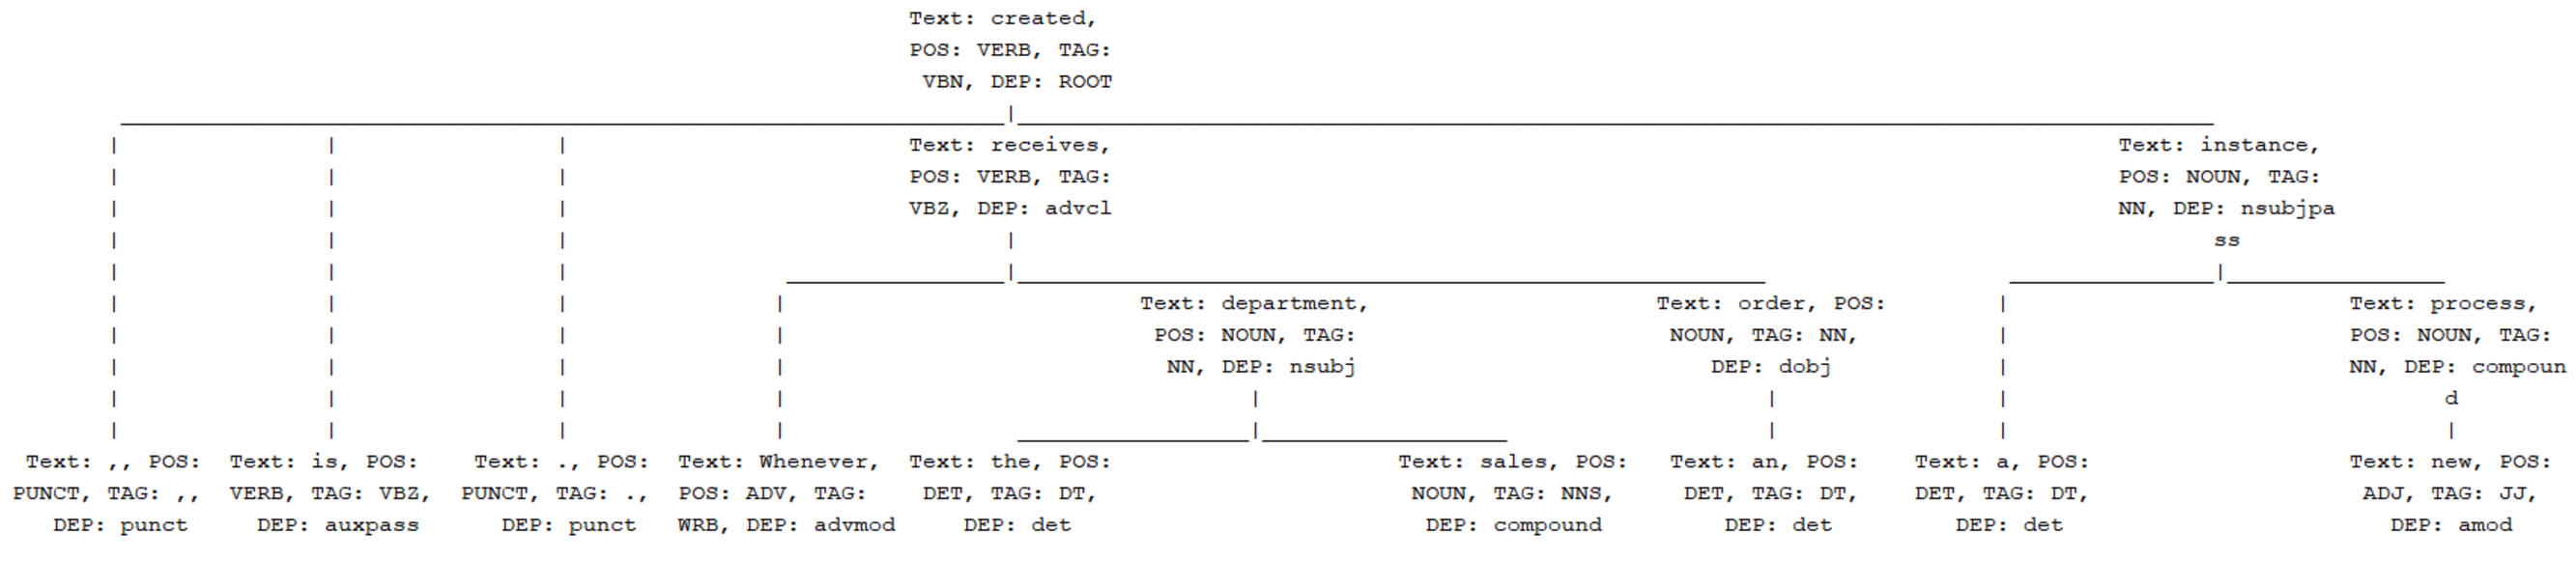
\includegraphics[width=\textwidth]{./images/participant_example.pdf}
	\caption{A syntax tree for the simple phrase \emph{``Whenever the sales department receives an order, a new process instance is created.''}}
	\label{fig:participant_example}
\end{figure}
{\scriptsize
\begin{longtable}{|p{0.03 \hsize}|p{0.25 \hsize}|p{0.15 \hsize}|p{0.2 \hsize}|p{0.1 \hsize}|p{0.1 \hsize}|}
	\hline
	Order & Activity & Condition & Who & Subprocess & Terminated.
	\\\hline\hline
	\csvreader[late after line=\\\hline]
	{./results/participant_example.csv}
	{Order=\Order,Activity=\Activity,Condition=\Condition,Who=\Who,Subprocess=\Subprocess,Terminated=\Terminated}
	{\Order & \Activity & \Condition & \Who & \Subprocess & \Terminated}
	\caption{Spreadsheet-based description generated from the sentence: \emph{``Whenever the sales department receives an order, a new process instance is created.''}}
	\label{csv:participant_example}
\end{longtable}
}
Listing~\ref{lst:participant_extraction} presents a Python script with the participant extraction implementation.\\
\lstinputlisting[language=Python, caption={Participant extraction function listing}, label={lst:participant_extraction}]{./listings/extract_participants.py}

\section{Subject-Verb-Object extraction}
\label{sec:svo}
After extracting the participants from the sentence, syntactic analysis in search of SVO (subject-verb-object) constructs is performed. These construct are used to generate intermediate process model.\\
First, the sentence is searched for \emph{``nsubj''} and \emph{``nsubjpass''} dependencies. For every word found, a new SVO construct is added to the output. In the case of words with nominal subject dependency, the subject is created from the extracted word, its predecessor in the syntax tree acts as a verb and the object is extracted from the subject's ancestors in syntax tree. The search for the object is divided into two phases.\\
First, a shallow search -- in which case only direct ancestors (children) in syntax sub-tree are analysed in search for tokens with two dependencies: \emph{``attr''} (attribute), \emph{``dobj''} (direct object). If object was not found during shallow search, a deep search (which involves all of the ancestors) with larger dependencies set -- \emph{``dobj''} (direct object), \emph{``iobj''} (indirect object), \emph{``pobj''} (object of preposition), \emph{``attr''} (attribute), \emph{``xcomp''} (open clausal complement). If the appropriate token is found, it is added as an object to SVO, otherwise the object part of SVO construct is omitted. Separating the object search into two phases improves the extraction results -- in most cases, the object is directly connected to the verb by \emph{``attr''} and \emph{``dobj''} dependency.  In case of tokens with nominal subject passive dependency, the object is omitted. For example, in the  sentence: \emph{``Purchase is registered''}, the word \emph{``Purchase''} is tagged as \emph{``nsubjpass''} and no object is present.\\
Similarly to the participants extraction, the SVO extraction also analyses the existence of conjunction in sentences. After finding a conjunction and validation its POS tag (this way, the conjunction which are not verbs are eliminated), it is used as a verb for a new SVO construct and the object is extracted from its children. Then, the syntax tree is analysed in search of the subject of a new construct. If the subject is found, a new SVO is created. This approach helps to deal with the sentences like: \emph{``If the storehouse has successfully reserved or backordered every item''}. In this case, by conjunction analysis it is possible to extract construct \emph{``backordered every item''}, which is conjoined by word \emph{``backordered''}.\\
In the last step, the extracted SVOs are connected with the corresponding participants, which were discovered by previous function in this sentence. Attaching participant to SVO will provide additional information during intermediate process model generation.\\
Figure~\ref{fig:svo_extraction_subprocess} shows BPMN diagram presenting overview of SVO extraction algorithm.
\begin{figure}[H]
	\centering
	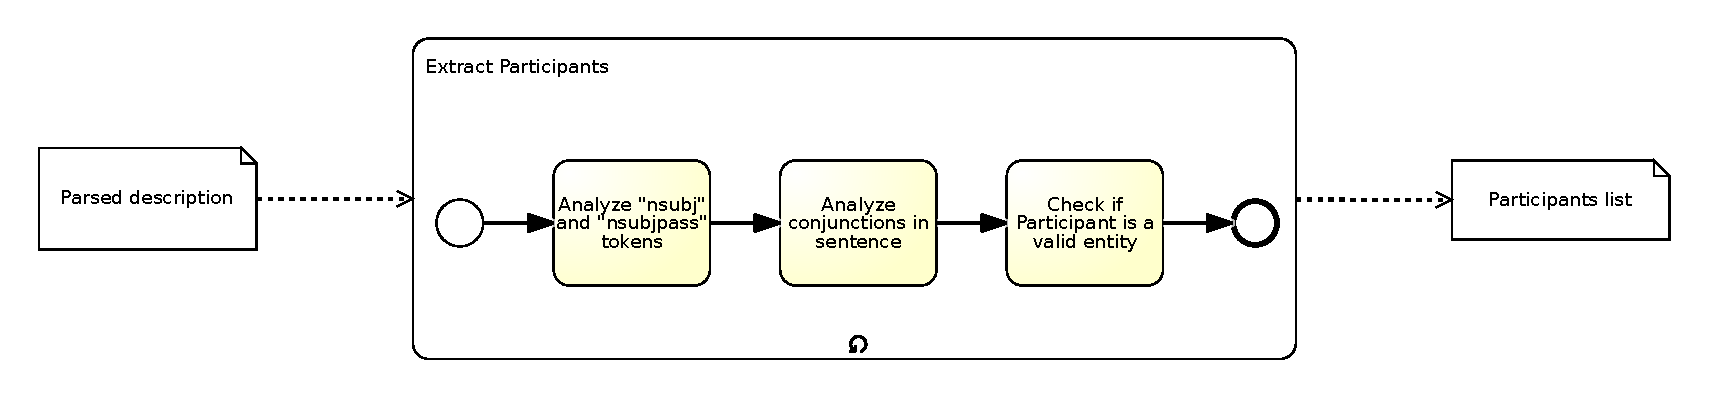
\includegraphics[width=\textwidth]{./images/participant_extraction_subprocess.pdf}
	\caption{BPMN diagram presenting overview of SVO extraction algorithm}
	\label{fig:svo_extraction_subprocess}
\end{figure}
Similarly to Participants, the SVOs have also a full name assigned. The difference lies in the accepted list of dependency labels. For the SVO, the following dependencies are used in full name (definitions of these dependencies are shown in Table~\ref{table:dependencies}):
\begin{itemize}
	\item amod, 
	\item acomp, 
	\item aux,
	\item auxpass,
	\item neg.
\end{itemize}
An example of SVO extraction is shown in Table~\ref{csv:svo_example}. In this case, a~simple sentence \emph{``Afterwards, the sales department ships the bicycle to the customer and finishes the process instance''} was processed. Two SVO constructs were extracted: \emph{``Sales Department ships bicycle''} and \emph{``Sales Department finishes process instance''}. The \emph{``Sales Department finishes process instance''} SVO was extracted using conjunction dependency, since the token \emph{``finishes''} is tagged with \emph{``conj''} dependency. In both cases, an appropriate participant (\emph{Sales Department}) was attached to activity and added to generated spreadsheet.
\begin{figure}[H]
	\centering
	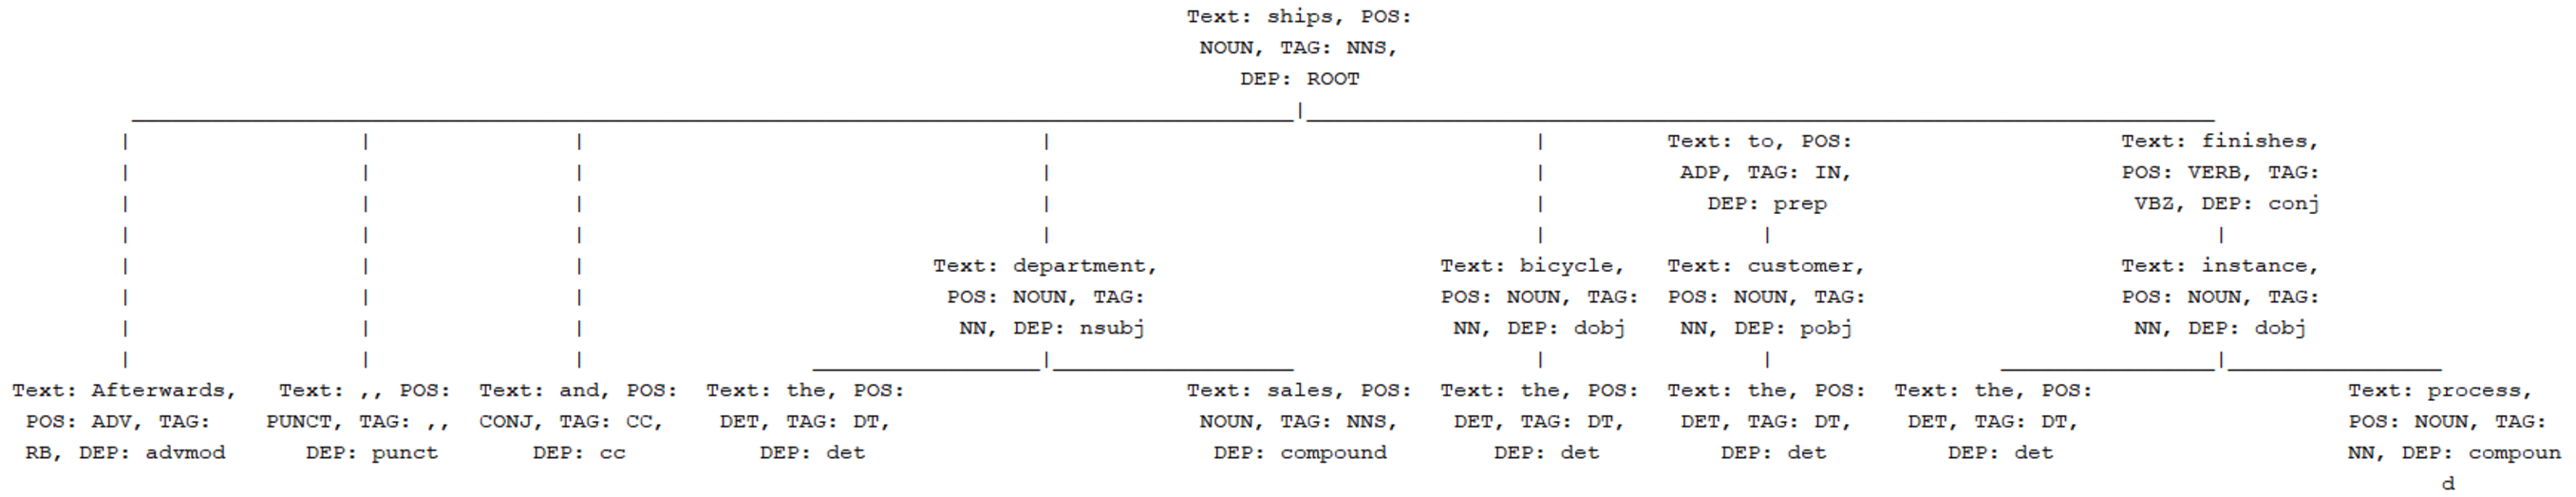
\includegraphics[width=\textwidth]{./images/svo_extraction_example.pdf}
	\caption{Syntax tree for simple phrase \emph{``Afterwards, the sales department ships the bicycle to the customer and finishes the process instance''}}
	\label{fig:svo_example}
\end{figure}
{\scriptsize
	\begin{longtable}{|p{0.03 \hsize}|p{0.25 \hsize}|p{0.15 \hsize}|p{0.2 \hsize}|p{0.1 \hsize}|p{0.1 \hsize}|}
		\hline
		Order & Activity & Condition & Who & Subprocess & Terminated.
		\\\hline\hline
		\csvreader[late after line=\\\hline]
		{./results/svo_extraction_example.csv}
		{Order=\Order,Activity=\Activity,Condition=\Condition,Who=\Who,Subprocess=\Subprocess,Terminated=\Terminated}
		{\Order & \Activity & \Condition & \Who & \Subprocess & \Terminated}
		\caption{Spreadsheet-based description generated from sentence: \emph{``Afterwards, the sales department ships the bicycle to the customer and finishes the process instance''}}
		\label{csv:svo_example}
	\end{longtable}
}
Listing~\ref{lst:svo_extraction} presents a Python script with SVO extraction implementation.\\
\lstinputlisting[language=Python, caption={Subject-Verb-Object extraction function listing}, label={lst:svo_extraction}]{./listings/extract_svo_constructs.py}

\section{Gateway keywords search}
After extracting the participants and subject-verb-object constructs, the whole description is analysed once more, in order to find keywords which indicate the existence of possible gateway. This function searches for three different types of keywords: conditional, parallel and default flow. The first type can be later translated either into an exclusive gateway or into an inclusive gateway, second -- into a parallel gateway. Third type might be used as a default flow of conditional gateway, provided that the correspondence with a conditional keyword will be found during model generation. If no correspondence is found, the SVO will be treated as a simple activity. The list of keywords are shown in Table~\ref{table:gateway-keywords}.\\
This function simply performs a word-by-word search of keywords. After finding one, the syntax tree is analysed in search of token which belongs to the SVO construct and which verb is a predecessor of keyword token that was found.\\
An example of conditional flow extracted from process description is shown in Table~\ref{csv:gateway_example}. A sentence \emph{``If the customer decides that the costs are acceptable, the process continues, otherwise she takes her computer home unrepaired.''} from the process description~\ref{txt:gateway_example} is translated into two activities, which are parts of conditional flow. Because the keyword associated with default flow was found and and activity with condition \emph{``else''} was added, a XOR gateway was added to the diagram.
\begin{tcolorbox}[
	breakable,
	arc=0mm,
	left=1pt,
	right = 1pt,
	boxrule=0mm,
	colback = {white},
	]
	\texttt{\input{./models/gateway_example.txt}}
\end{tcolorbox}
\captionof{textdesc}{Fragment of a process description with extractable conditional gateway}
\label{txt:gateway_example}
{\scriptsize
	\begin{longtable}{|p{0.03 \hsize}|p{0.20 \hsize}|p{0.15 \hsize}|p{0.1 \hsize}|p{0.1 \hsize}|p{0.1 \hsize}|}
		\hline
		Order & Activity & Condition & Who & Subprocess & Terminated.
		\\\hline\hline
		\csvreader[late after line=\\\hline]
		{./results/gateway_example.csv}
		{Order=\Order,Activity=\Activity,Condition=\Condition,Who=\Who,Subprocess=\Subprocess,Terminated=\Terminated}
		{\Order & \Activity & \Condition & \Who & \Subprocess & \Terminated}
		\caption{Spreadsheet-based description generated from a text description shown in Text~\ref{txt:gateway_example}}
		\label{csv:gateway_example}
	\end{longtable}
}
\begin{figure}[H]
	\centering
	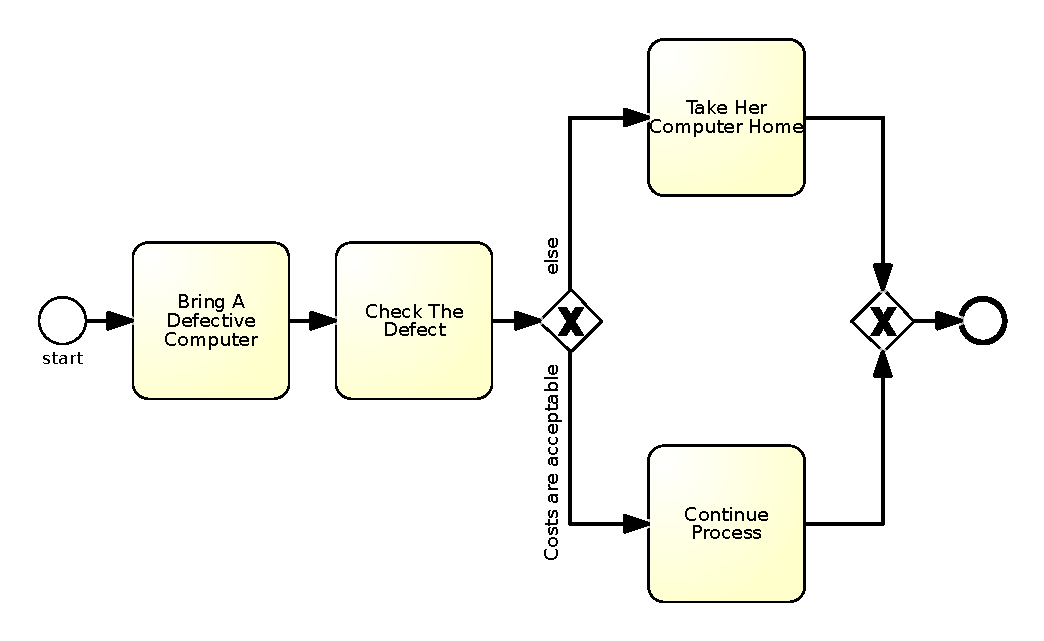
\includegraphics[scale=0.55]{./images/gateway_example.pdf}
	\caption{BPMN diagram with an XOR gateway, generated from the intermediate process model shown in Table~\ref{csv:gateway_example}}
	\label{fig:gateway_example}
\end{figure}
The Listing~\ref{lst:gateway_extraction} presents a Python script with gateway keywords extraction implementation.
\lstinputlisting[language=Python, caption={Gateway keywords search function listing}, label={lst:gateway_extraction}]{./listings/find_gateway_keywords.py}

\section{Prototype model generation}

\subsection{Intermediate model description}
The prototype implementation uses a spreadsheet-based process description, which employs a CSV (Comma-Separated Values) file format to represent a business process model. This spreadsheet-based process description is presented in the article~\cite{kluza-spreadsheet}. A business process is described by a spreadsheet table. Each row represents a single phase, which can be translated into a BPMN task or sub-process. Columns represent the properties of each phase. Overall, there are six properties:
\begin{itemize}
	\item Order -- number of the corresponding phase. Parallel or excluding tasks are distinguished by suffix created from the consecutive letters (a-z). In the case of nested gateways, another suffix, with number of phase and letter for branch is added. Table~\ref{csv:csv_order_example} shows an example of spreadsheet-based process model. Notice that activities \emph{``Initiate search''} and \emph{``Track files''} are parts of conditional flow, thus the order number has a branch suffix added,
	
	{\scriptsize
		\begin{longtable}{|p{0.03 \hsize}|p{0.25 \hsize}|p{0.15 \hsize}|p{0.2 \hsize}|p{0.1 \hsize}|p{0.1 \hsize}|}
			\hline
			Order & Activity & Condition & Who & Subprocess & Terminated.
			\\\hline\hline
			\csvreader[late after line=\\\hline]
			{./results/csv_order_example.csv}
			{Order=\Order,Activity=\Activity,Condition=\Condition,Who=\Who,Subprocess=\Subprocess,Terminated=\Terminated}
			{\Order & \Activity & \Condition & \Who & \Subprocess & \Terminated}
			\caption{Spreadsheet-based description generated from sentence: \emph{``Afterwards, the sales department ships the bicycle to the customer and finishes the process instance''}}
			\label{csv:csv_order_example}
		\end{longtable}
	}

	\item Activity -- name of the performed action. There is a special case -- \emph{``goto X''} is a special statement, which signalizes that a part of the process must be skipped or there is a loop in a process. Table~\ref{csv:activity_csv_example} shows an example of spreadsheet-based process model. Notice the special statement \emph{``goto 5''} in activity \emph{4b1},
	
	{\scriptsize
		\begin{longtable}{|p{0.03 \hsize}|p{0.25 \hsize}|p{0.15 \hsize}|p{0.2 \hsize}|p{0.1 \hsize}|p{0.1 \hsize}|}
			\hline
			Order & Activity & Condition & Who & Subprocess & Terminated.
			\\\hline\hline
			\csvreader[late after line=\\\hline]
			{./results/csv_activities_example.csv}
			{Order=\Order,Activity=\Activity,Condition=\Condition,Who=\Who,Subprocess=\Subprocess,Terminated=\Terminated}
			{\Order & \Activity & \Condition & \Who & \Subprocess & \Terminated}
			\caption{An example of spreadsheet-based process model with multiple activities}
			\label{csv:activity_csv_example}
		\end{longtable}
	}
	
	\item Condition -- a condition, which has to be fulfilled in order to perform the task. This property is used to implement the exclusive and inclusive gateway. In the first case, a gateways should consist of at least two tasks, one of which should be filled with condition. The last one from all of the tasks that belong to the gateway should contain a keyword \emph{``else''} as a condition. In case of inclusive gateway, both tasks should contain the corresponding conditions. Table~\ref{csv:gateway_csv_example} shows an example of spreadsheet-based process model with conditional flow included. In this case, activities \emph{``Approve Loan''} and \emph{``Deny Loan''} will be connected by inclusive gateway, since both activities have a condition and there is not \emph{``else''} keyword,
	
	{\scriptsize
		\begin{longtable}{|p{0.03 \hsize}|p{0.20 \hsize}|p{0.15 \hsize}|p{0.1 \hsize}|p{0.1 \hsize}|p{0.1 \hsize}|}
			\hline
			Order & Activity & Condition & Who & Subprocess & Terminated.
			\\\hline\hline
			\csvreader[late after line=\\\hline]
			{./results/csv_condition_example.csv}
			{Order=\Order,Activity=\Activity,Condition=\Condition,Who=\Who,Subprocess=\Subprocess,Terminated=\Terminated}
			{\Order & \Activity & \Condition & \Who & \Subprocess & \Terminated}
			\caption{Spreadsheet-based description with conditional flow included}
			\label{csv:gateway_csv_example}
		\end{longtable}
	}
	
	\item Who – the name of person, system or department responsible for executing this phase. This property can be transformed into a swimlane in BPMN diagram,
	\item Subprocess -- this property informs that a task should be considered as a sub-process. This column should be filled with \emph{``yes''} (if the task is a sub-process), or left empty otherwise,
	\item Terminated -- this property informs that a given task terminates the process. This column should be filled with \emph{``yes''} if this is the case.
\end{itemize}
The spreadsheet-based process description presented in article~\cite{kluza-spreadsheet} supports only basic BPMN elements. However, the subset of supported BPMN elements covers the most commonly used elements of BPMN diagram~\cite{bpmn-stats}. Moreover, the supported subset covers all of the elements required for the purpose of this thesis as well.
\begin{figure}
	\centering
	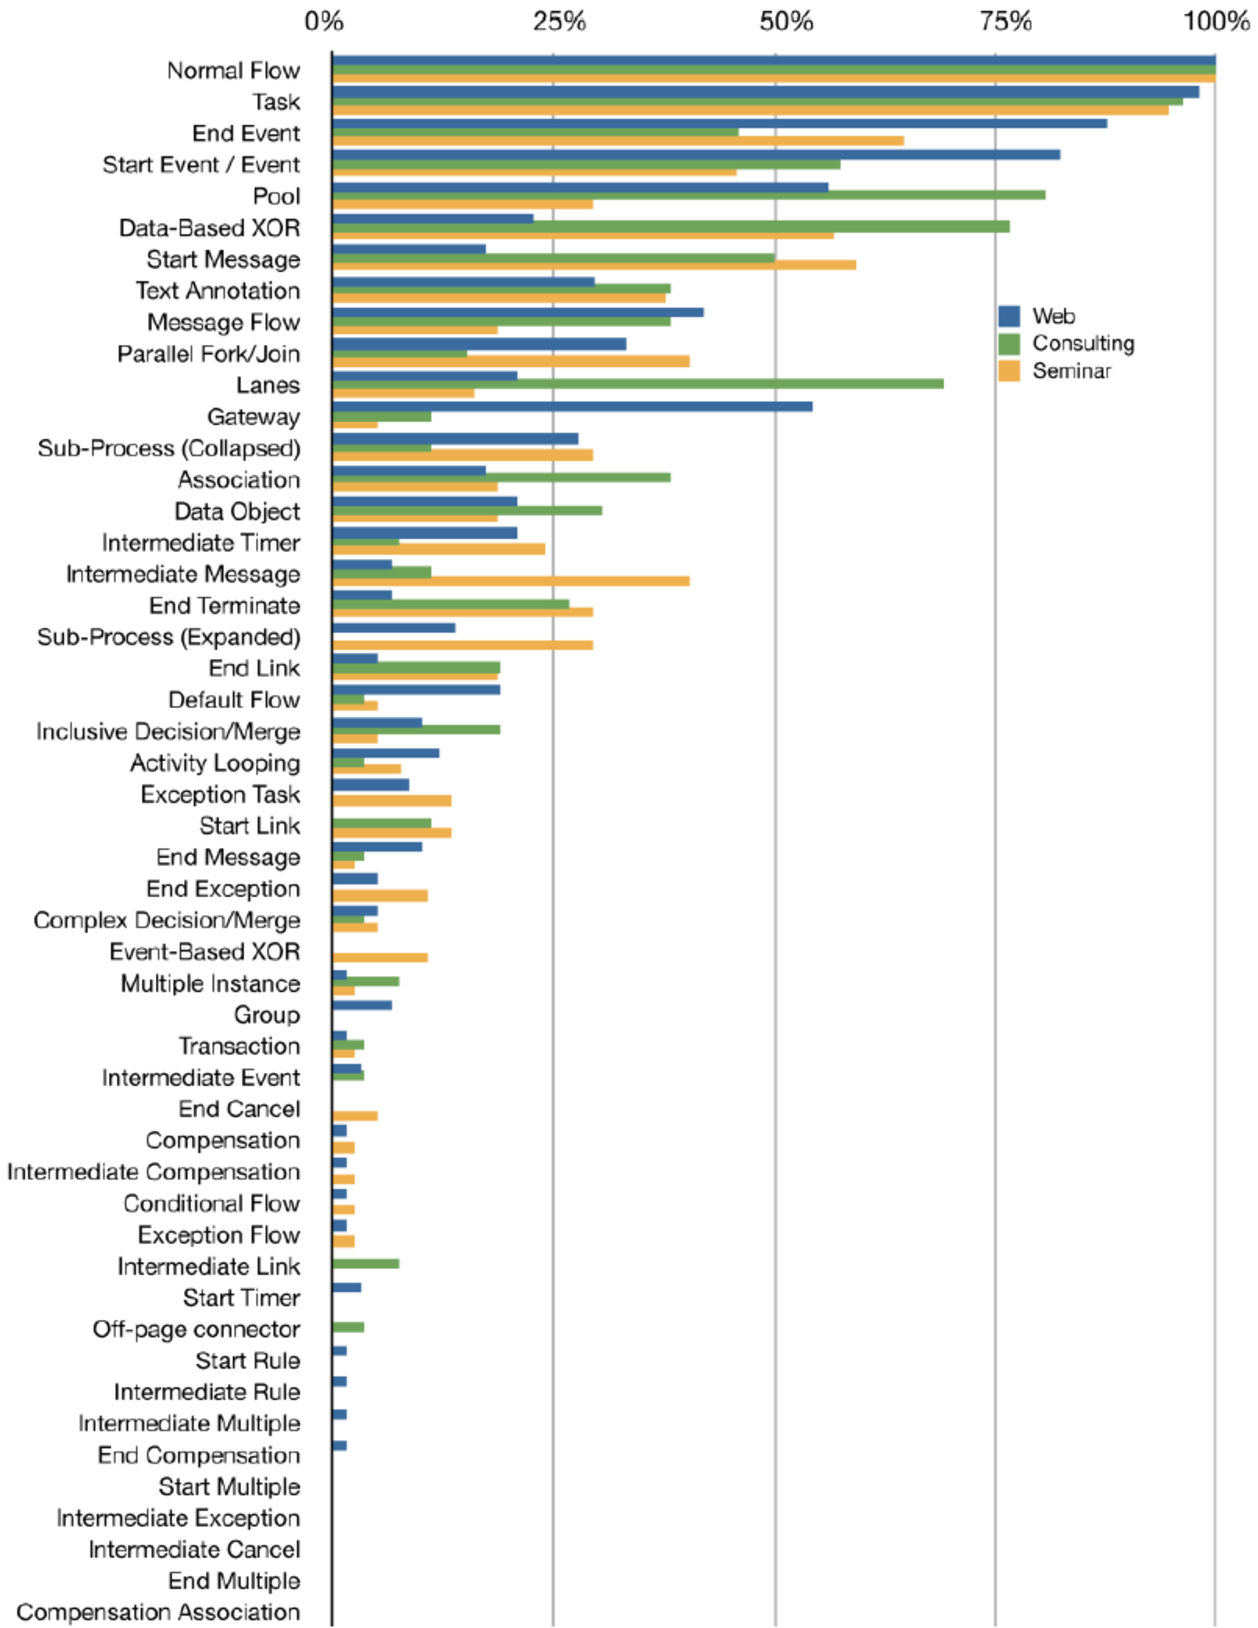
\includegraphics[width=\textwidth]{./images/bpmn_usage_stats.pdf}
	\caption{Frequency of occurrence diagram for BPMN elements. Diagram obtained from article~\cite{bpmn-stats}}
	\label{fig:bpmn_usage_stats}
\end{figure}

\subsection{Spreadsheet-based model generation approach}
The final part of the implemented prototype is the intermediate process model generation phase. This phase makes use of previous functions to discover information useful for process model. As it was said earlier, the final product of this phase is a spreadsheet-based model, which is used to generate BPMN diagram and can be revised by a human expert.\\
Before the extraction process begins, a simple text preprocessing is performed. It basically consists of two actions:
\begin{itemize}
	\item removing all newlines and replacing them with whitespaces,
	\item removing hyphens from the description.
\end{itemize}
Both of these steps are performed in order to fix some of the parser issues. The presence of newline characters (\emph{``\texttt{\textbackslash n}''} used in operating systems based on Unix core and \emph{``\texttt{\textbackslash r\textbackslash n}''} in operating systems from Windows family) results in the situation where sentences are incorrectly split -- newline is treated as a~single, empty sentence, and it breaks the sentences into two unrelated pieces. Removal of hyphens is performed in order to fix the issue with compound verbs and adjectives (such as "pre-sales"). Compounds are split into multiple words during syntax parsing, which makes the extraction of Participant or SVO full name difficult -- some of the information may be lost.\\
In the first phase, the elements (participants and SVO) extraction is performed. Next, the gateway keywords search proceeds. After these initial steps, the list of process activities is initialized -- start activity is inserted. Next, the Subject-Verb-Object constructs are sorted by their chronological appearance in the text. After that, the program iterates over a list of extracted SVO. For each construct, the appropriate action, based on a set of conditions, should be performed:
\begin{itemize}
	\item if the SVO is labelled with a conditional gateway keyword, it is added to the intermediate model as a part of conditional gateway. If there was a parallel gateway detected earlier, the appropriate flag is set to false. Next, the conditional gateway is initialized by setting up the conditional gateway flag and helper variables. The usage of gateway flag helps to deal with sentences such as \emph{``If <first condition>, <action>. If <second condition>, <action>''} which should be treated as a parts of single gateway. After the initialization, current SVO and next one from the list are added to the model as a condition-action of a conditional gateway. This part works under the assumption, that the condition (also extracted as a SVO) is mentioned before action. In compliance to the intermediate model requirements, the property \emph{``Condition''} is filled with a full name of the condition SVO. If the condition SVO has a participant attached and it is not a pronoun, the full name of participant is entered as the \emph{``Who''} property. Otherwise, it is left empty,
	\item SVO labelled with a parallel gateway keyword is treated in a similar way. The main difference is that after initialization, the next SVO from a list is added as a parallel task to the current SVO. This approach should work with simple sentences, such as \emph{``while <action one>, <action two>''}, in which the parallel tasks are mentioned consecutively. Similarly to the conditional gateway rule, if the inserted actions has a participant attached and it is not a pronoun, the \emph{``Who''} property is filled with its full name or left empty otherwise,
	\item if the SVO is labelled as default flow, the behaviour of function depends on previously detected gateways. If the parallel gateway was found, the SVO is added as another task in this gateway. For the conditional gateway, a default flow is added -- an additional task, with keyword \emph{``else''} entered as a \emph{``Condition''} property. A default flow is recognized by the keyword \emph{``else''} in condition column. If none of the gateways were added previously, the SVO is added as a simple task. This option was added, so that the potentially useful information would not be lost. The SVO will be added as a task, provided that it has a validated participant attached. This is performed in order to filter out the unnecessary SVO, which should not be treated as tasks, but only provides some information about conditions in gateways or other descriptive information. In all of these cases, the participant attached to the action is treated exactly like in previous options,
	\item if none of the previous options were executed, the SVO is added as a simple task, connected by a sequence flow. Before a new task is added, gateway flags are checked. In the case of parallel gateway flag, it is set to false. In case of the conditional gateway flag, a gateway branch index is evaluated. If it is lower that two, a default flow (activity with \emph{``Condition''} set to \emph{``else''}), which points to the end event (which is achieved by naming the activity as \emph{``goto X''}, where X is a current value of order, incremented by one), is added to the gateway. This is performed due to the fact, that the conditional gateway with one conditional flow, will result in deadlock -- if the only condition is false, the process cannot be continued. After this check, the SVO construct can be added as a~simple task. The participant attached is handled similarly like in previous situations.
\end{itemize}
Figure~\ref{fig:intermediate_model_generation} shows the BPMN diagram presenting overview of intermediate process model description generation algorithm.\\
\begin{figure}
	\centering
	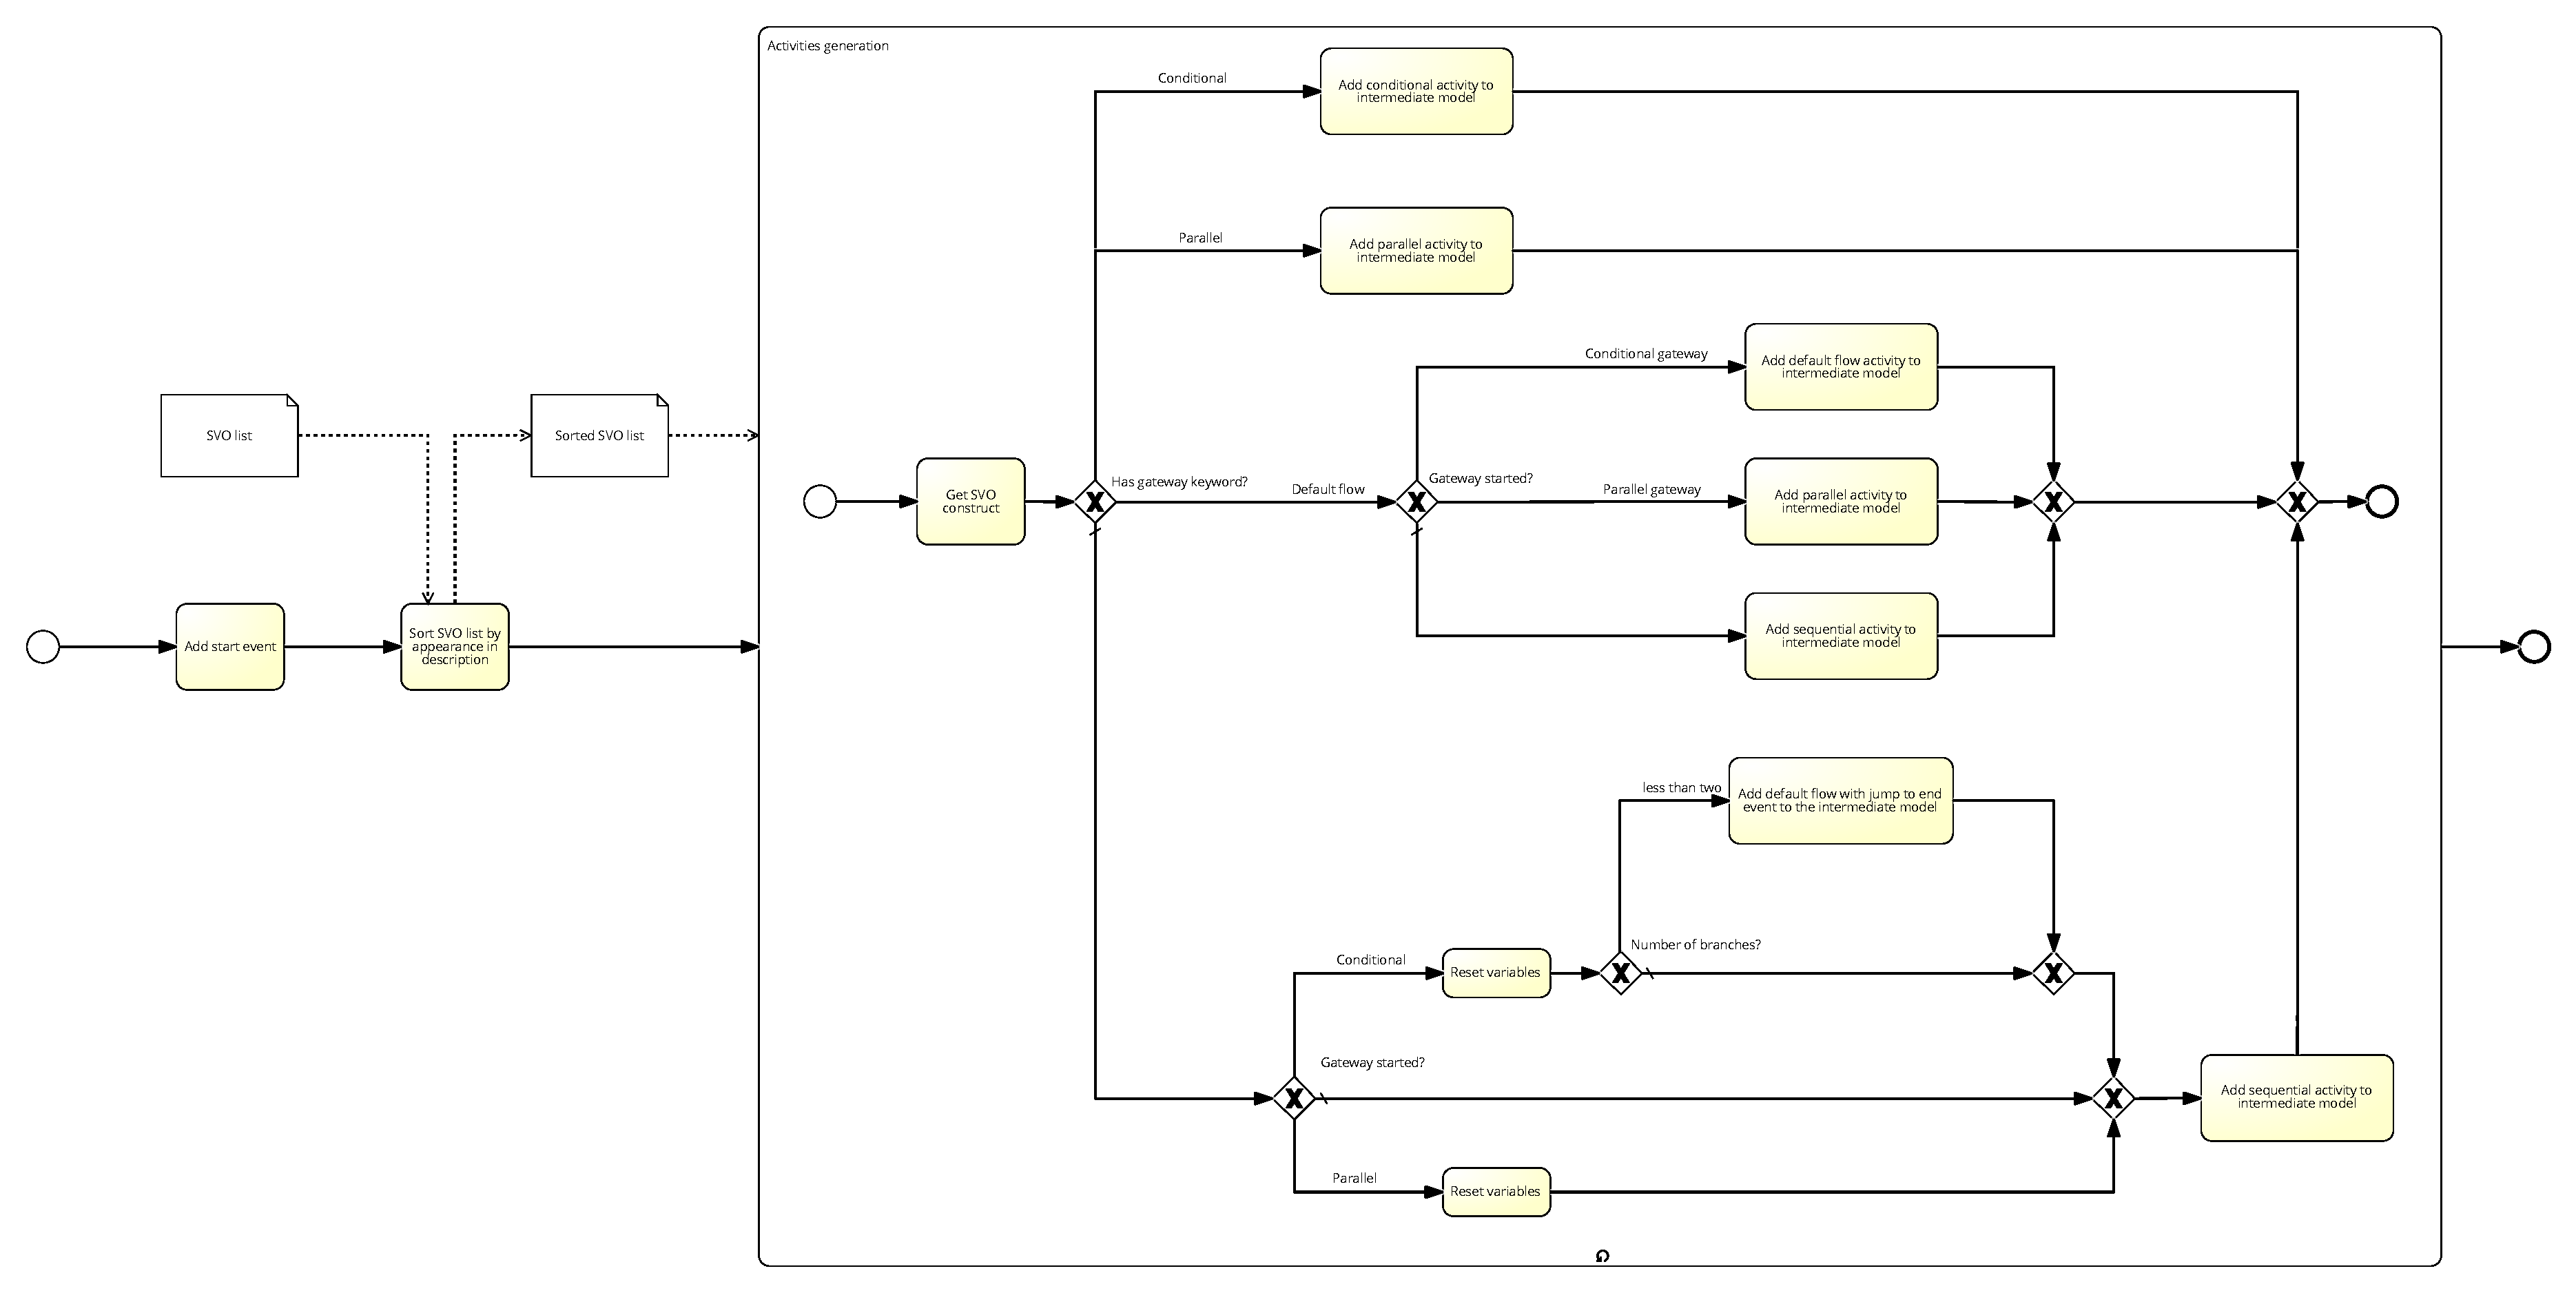
\includegraphics[width=0.95\textheight, angle=90]{./images/intermediate_model_generation.pdf}
	\caption{BPMN diagram presenting overview of intermediate process model description generation algorithm}
	\label{fig:intermediate_model_generation}
\end{figure}
After all of the subject-verb-objects constructs are processed, the conditional gateway flag is validated once more -- similarly to the last case, if conditional gateway has only one conditional flow, a default flow is added. Finally, the end event is added, which finishes the intermediate process generation.\\
Before a new activity is added to the intermediate model, the SVO which serves as a basis for the activity is validated. Validation process checks if the base form of verb part of SVO belongs to one of two sets of specific verbs. The first set is called \emph{``ignorable verbs''} and consists of verbs such as \emph{``need''}, \emph{``exist''}. Using this set, it is possible to discard SVO that clearly should not be converted into activity, since these SVO does not provide any information about the activity. An example of such SVO is \emph{``Customer does not exist''} which does not indicate any activity that should be performed -- this SVO might rather be used as a condition. The second set, called \emph{``replaceable verbs''} contains verbs like \emph{``be''} or \emph{``do''}. These verbs indicate that SVO might contain information about possible activity, but the correct verb should be found. The search is performed by checking the verb token syntax sub-tree in search of token tagged with \emph{VERB} POS tag, which is neither ignorable or replaceable verb. An example of SVO which includes the replaceable verb, but can be converted into activity can be phrase \emph{``Patient is examined''}. This SVO can be converted into valid activity \emph{``Examine Patient''}. An example of SVO which includes the replaceable verb, but do not provide information about activity, can be phrase \emph{``Part is available''}. This SVO could be used as a condition of the gateway, but is not a valid activity.\\
After checking if SVO should be converted into an activity, the conversion process begins. First, it is decided whether activity should be ordered as Verb-Subject or Verb-Object. If the object is missing from SVO or it is tagged as \emph{VERB}, the former is chosen. Otherwise, the Verb-Object form is chosen. This allows to distinct between phrases such as \emph{``Process instance is created''} and \emph{``Sales department receives an order''}. In the first case, the Verb-Subject form is chosen and an activity \emph{``Create Process Instance''} is generated. In the second case, an activity \emph{``Receive Order''} is created. The verb in activity is always turned into base form. Additional words appear in activity name, because verb and subject or object are printed by full name -- adding tokens with specific dependencies, as described in sections~\ref{sec:participant} and~\ref{sec:svo}. These two simple rules of creating activity name should provide a proper descriptions in most cases.

{\scriptsize
	\begin{longtable}{|p{0.03 \hsize}|p{0.25 \hsize}|p{0.15 \hsize}|p{0.2 \hsize}|p{0.1 \hsize}|p{0.1 \hsize}|}
		\hline
		Order & Activity & Condition & Who & Subprocess & Terminated.
		\\\hline\hline
		\csvreader[late after line=\\\hline]
		{./results/participant_example.csv}
		{Order=\Order,Activity=\Activity,Condition=\Condition,Who=\Who,Subprocess=\Subprocess,Terminated=\Terminated}
		{\Order & \Activity & \Condition & \Who & \Subprocess & \Terminated}
		\caption{Spreadsheet-based description generated from sentence: \emph{``Whenever the sales department receives an order, a new process instance is created.''}. Notice that the activities in generated model are derivation of SVO extracted from sentence.}
		\label{csv:activity_example}
	\end{longtable}
} 

The Python script for intermediate process model description generation is shown in Listing~\ref{lst:intermediate_model_generation}.
\lstinputlisting[language=Python, caption={Intermediate process model generation function listing}, label={lst:intermediate_model_generation}]{./listings/generate_intermediate_model.py}

\section{BPMN diagram generation}
The spreadsheet-based model can be used to generate a BPMN diagram, using functionality provided by \emph{bpmn\_python} -- a library written in Python, in order to provide a functionality to import and export BPMN diagrams in XML file format. In addition, a manual diagram generation functionality was added as well. As a part of other student project, a functionality for importing spreadsheet-based model description was implemented into the \emph{bpmn\_python} library. This library allows a user to export the imported diagram (stored as a graph structure) into a valid BPMN 2.0 XML file. Using these functionalities, the intermediate models are translated into diagrams, which finishes the process of translating a natural language description into a BPMN diagram. Detailed informations about \emph{bpmn\_python} package with simple user guide added will be presented in Appendix~\ref{cha:bpmn-python}.\\
Detailed description of translating spreadsheet-based model into BPMN diagram will be presented on example from test data set in section~\ref{sec:detailed-example}.\\
This section presented the business process extraction and BPMN diagram generation method details, describing step-by-step the algorithms used in prototype. Next section describes the validation approach and results of implemented prototype validation.
\chapter{Results}
\label{cha:validation}
\section{Test data set}
Evaluation of implemented prototype was performed using a set of textual process description with corresponding hand-made process diagram. This data set was introduced in article~\cite{friedrich-2011}. Thirty-two models from the introduced data set were used to evaluate proposed method. This subset contains the descriptions and models introduced in academic textbooks~(\cite{white-bpmn-reference-guide},~\cite{praxishandbuch}), BPMN modelling tutorials and industrial sources (websites and on-line help documentation of BPM tool vendors -- Active VOS, Oracle, and BizAgi). The academic models introduced in~\cite{friedrich-2011} were provided by a courtesy of the Humboldt Universit at zu Berlin, the Technishe Universit at Berlin, the Queensland University of Technology.

\section{Validation methodology}
The generated models were compared with hand-made models  in two ways:
\begin{itemize}
	\item using a set of complexity metrics introduced in several papers -- this way it is possible to numerically compare the structure of models,
	\item by manual analysis of hand-made and generated models.
\end{itemize}
The complexity metrics used in evaluation method were introduced in several articles. Those metrics are:
\begin{itemize}
	\item Number Of Activities in a process (\texttt{NOA}) and Number Of Activities and Control-flow elements (\texttt{NOAC}) were introduced by Cardoso et al. in~\cite{cardoso-metrics}. Those basic metrics simply returns information about number of basic process elements in process model -- activities, in case of \texttt{NOA} metric, activities and control flow elements (gateways , events) in case of \texttt{NOAC} metric. For the purpose of the proposed method evaluation, \texttt{NOAC} metric is not directly used -- rather, a variation of \texttt{NOAC}, which returns only a number of control flow elements is used. This metric will labelled \texttt{NOC} -- Number Of Control-flow elements. Using \texttt{NOA} and \texttt{NOC} metrics it is possible to compare number of activities and control flow elements separately,
	\item Coefficient of Network Complexity (\texttt{CNC}) metric introduced by Latva-Koivisto in~\cite{latva-metric}. \texttt{CNC} can be used to measure the degree of complexity of a critical pass network. The formula of CNC can be described by equation $ (number\_of\_arcs)/(number\_of\_activities\_joins\_and\_splits) $,
	\item Average Gateway Degree~(\texttt{Avg}) -- Average of the number of both incoming and outgoing arcs of the gateway
	nodes in the process model. This metric was introduced in~\cite{sanchez-metric},
	\item Gateway Heterogeneity~(\texttt{Heter}) -- Number of different types of gateways used in a model. This metric was introduced in~\cite{sanchez-metric}.
\end{itemize}
Using this set of the complexity metric, it should be possible to compare the structural differences between manually created and generated models. Additionally, the generated models were manually analysed and compared with hand-made models in order to find limitations and weaknesses of implemented method.

\section{Validation results}

\subsection{Metrics value analysis}
Detailed metrics values for each model are presented in tables~\ref{csv:metrics_part_one} and~\ref{csv:metrics_part_two}. Table~\ref{csv:metrics_part_one} presents the values of \texttt{NOA} and \texttt{NOC} metrics. This table is structured in this way:
\begin{itemize}
	\item first column shows a model name,
	\item columns number two to number four present values of \texttt{NOA} metric for hand-made model (column \texttt{NOA-H}), generated model (column \texttt{NOA-G}), difference between \texttt{NOA} metric for hand-made model and for generated model (column \texttt{NOA-diff}). Fifth column shows the proportion of difference between \texttt{NOA} metrics proportional to \texttt{NOA} metric for hand-made model (column \texttt{NOA-prop}),
	\item columns number six to number nine are organized in similar manner to previous part, but present values of \texttt{NOC} metric. Columns are named in the similar way (\texttt{NOC-H}, \texttt{NOC-G}, \texttt{NOC-diff}, \texttt{NOC-prop}).
\end{itemize}
Difference between metrics indicates whether the number of corresponding elements (activities or control flow elements) in the generated model were lower (when difference is positive number) or higher (when difference is a negative number) than in the hand-made model. Table~\ref{csv:noa_noc_max_min} shows the minimum and maximum values of metrics (with the name of corresponding model), listing difference and  proportional difference separately.
\newpage
{\scriptsize
	\begin{longtable}{|p{0.09 \hsize}|p{0.08 \hsize}|p{0.08 \hsize}|p{0.08 \hsize}|p{0.08 \hsize}|p{0.08 \hsize}|p{0.08 \hsize}|p{0.08 \hsize}|p{0.09 \hsize}|}
		\hline
		Model name & NOA-H & NOA-G & NOA-diff & NOA-prop & NOC-H & NOC-G & NOC-diff & NOC-prop
		\\\hline\hline
		\csvreader[late after line=\\\hline]
		{./results/metrics_part_one.csv}
		{Model name=\CA,NOA-H=\CB,NOA-G=\CC,NOA-diff=\CD,NOA-prop=\CE,NOC-H=\CF,NOC-G=\CG,NOC-diff=\CH,NOC-prop=\CI}
		{\CA & \CB & \CC & \CD & \CE & \CF & \CG & \CH & \CI}
		\caption{Validation results -- NOA and NOC metrics}
		\label{csv:metrics_part_one}
	\end{longtable}
}
\begin{table}[H]
	{\small
	\centering
	\begin{tabular}{|p{0.14 \textwidth}|p{0.15 \textwidth}|p{0.2 \textwidth}|p{0.15 \textwidth}|p{0.2 \textwidth}|}
		\hline
		Metric & Min. difference & Model & Max. difference & Model \\
		\hline
		NOA & -47 & Model 5 & 1 & Model 31 \\
		\hline
		NOA (prop.) & -380.00\% & Model 18 & 12.50\% & Model 31 \\
		\hline
		NOC & -4 & Model 18 & 28 & Model 5 \\
		\hline
		NOC (prop.) & -200.00\% & Model 18 & 90.32\% & Model 6 \\
		\hline
	\end{tabular}
	}
	\caption{Minimum and maximum values of NOA and NOC metrics}
	\label{csv:noa_noc_max_min}
\end{table}
Analysis of results shown in tables~\ref{csv:metrics_part_one}~and~\ref{csv:noa_noc_max_min} shows that most of the generated models have higher number of activities (higher \texttt{NOA} metric) and lower number of control flow elements (lower \texttt{NOC} metric) than the hand-made models. Average of proportional difference between \texttt{NOA} metrics equals to $ -87.50\% $. Average of difference between \texttt{NOC} metrics equals to $ 31.74\% $. Model number eighteen is an extreme case, having nearly five times more activities than corresponding hand-made models -- while the hand-made model have only five activities, the generated model consists of twenty four activities. In case of \texttt{NOC} metric, the extreme values are a bit confusing. While the lowest proportional difference is $ -200\% $, meaning that the generated model has three times more of control flow elements than hand-made model, the actual numbers of control flow elements are two (in case of hand-made model) and six (in case of generated model). In most cases, the hand-made model consists of more control flow elements than the generated one.\\
To summarize the analysis of \texttt{NOA} and \texttt{NOC} metrics:
\begin{itemize}
	\item in case of \texttt{NOA} metric, the generated models had higher value of this metric in twenty nine cases, equal value to the hand-made model in two cases (models number three and twenty-eight) and lower value in one case (model number thirty-one),
	\item in case of \texttt{NOC} metric, the generated models had higher value of this metric in two cases (models number sixteen and eighteen), equal value to the hand-made model in six cases (models number seven, nine, thirteen, seventeen, twenty and twenty-four) and lower value in twenty-four cases.
\end{itemize}
\begin{figure}[p]
	\centering
	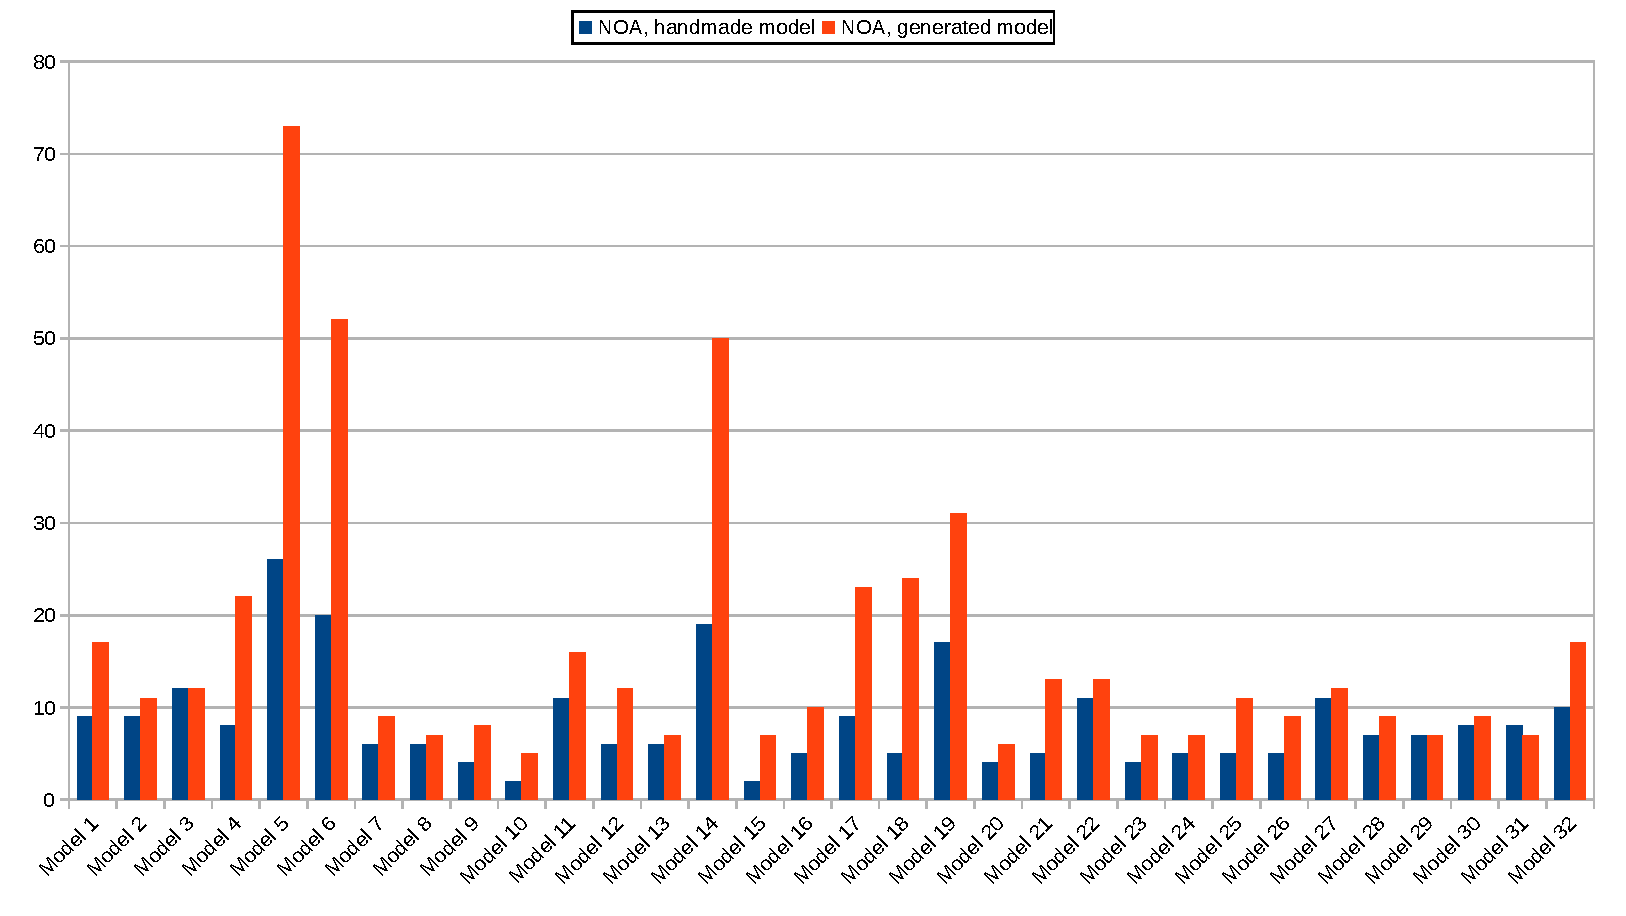
\includegraphics[width=0.95\textheight, angle=90]{./images/noa_chart.pdf}
	\caption{Chart showing comparison of NOA metric between models}
	\label{bpmn:noa_chart}
\end{figure}
\begin{figure}[p]
	\centering
	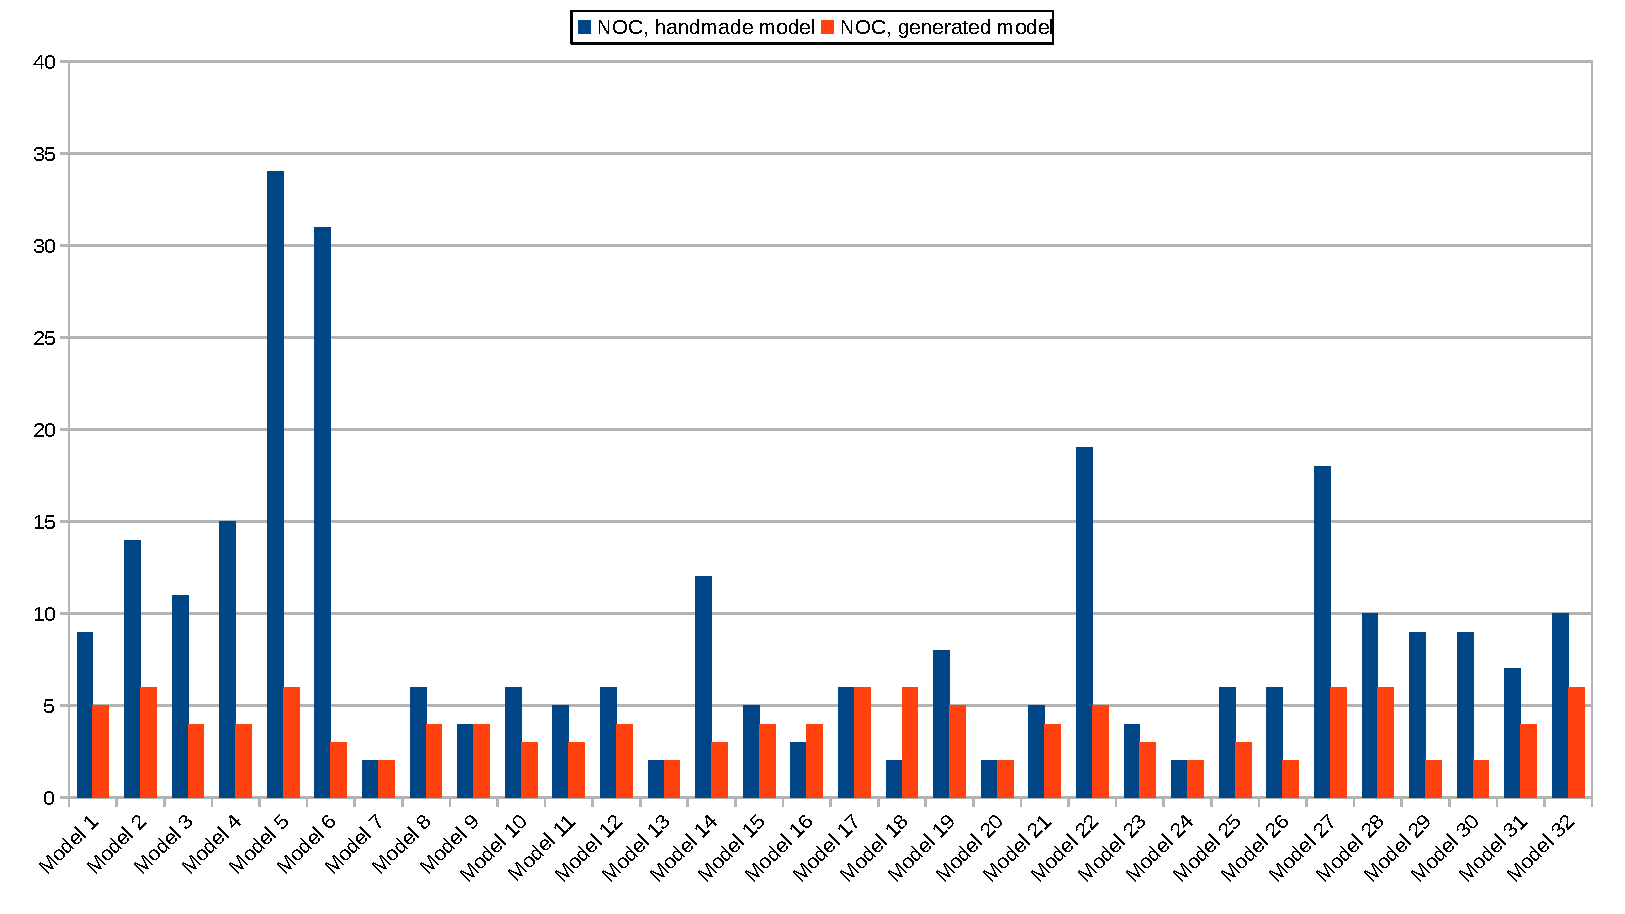
\includegraphics[width=0.95\textheight, angle=90]{./images/noc_chart.pdf}
	\caption{Chart showing comparison of NOC metric between models}
	\label{bpmn:noc_chart}
\end{figure}
Table~\ref{csv:metrics_part_two} presents the values of Coefficient of Network Complexity, Average Gateway Degree and Gateway Heterogeneity metrics. This table is structured in this way:
\begin{itemize}
	\item first column shows a model name,
	\item columns number two to number four present values of \texttt{CNC} metric for hand-made model (column \texttt{CNC-H}), generated model (column \texttt{CNC-G}), absolute difference between \texttt{CNC} metric for hand-made model and for generated model (column \texttt{CNC-diff}),
	\item columns number five to number seven are similar to previous part but present values of Average Gateway Degree metric. Columns are named in the similar way (\texttt{Avg-H}, \texttt{Avg-G}, \texttt{Avg-diff}),
	\item columns number five to number seven are similar to previous part but present values of Gateway Heterogeneity metric. Columns are named in the similar way (\texttt{Heter-H}, \texttt{Heter-G}, \texttt{Heter-diff}).
\end{itemize}
\newpage
{\scriptsize
	\begin{longtable}{|p{0.09 \hsize}|p{0.07 \hsize}|p{0.07 \hsize}|p{0.08 \hsize}|p{0.07 \hsize}|p{0.07 \hsize}|p{0.08 \hsize}|p{0.07 \hsize}|p{0.07 \hsize}|p{0.07 \hsize}|}
		\hline
		Model name & CNC-H & CNC-G & CNC-diff & Avg-H & Avg-G & Avg-diff & Heter-H & Heter-G & Heter-diff
		\\\hline\hline
		\csvreader[late after line=\\\hline]
		{./results/metrics_part_two.csv}
		{Model name=\CA,CNC-H=\CB,CNC-G=\CC,CNC-diff=\CD,Avg-H=\CE,Avg-G=\CF,Avg-diff=\CG,Heter-H=\CH,Heter-G=\CI,Heter-diff=\CJ}
		{\CA & \CB & \CC & \CD & \CE & \CF & \CG & \CH & \CI & \CJ}
		\caption{Validation results -- Coefficient of Network Complexity, Average Gateway Degree and Gateway Heterogeneity metrics}
		\label{csv:metrics_part_two}
	\end{longtable}
}
\begin{table}[H]
	{\small
	\centering
	\begin{tabular}{|p{0.2 \hsize}|p{0.15 \hsize}|p{0.15 \hsize}|p{0.1 \hsize}|p{0.15 \hsize}|p{0.1 \hsize}|}
		\hline
		Metric & Avg. difference & Min. difference & Model & Max. difference & Model \\
		\hline
		CNC & 0.019 & -0.305 & Model 27 & 0.591 & Model 26 \\
		\hline
		Avg. Gateway Degree & 0.058 & -4.000 & Model 18 & 3.000 & Model 26 \\
		\hline
	\end{tabular}
	}
	\caption{Average, minimum and maximum values of Coefficient of Network Complexity and Average Gateway Degree metrics}
	\label{csv:cnc_avg_heter_max_min}
\end{table}
Analysis of results shown in tables~\ref{csv:metrics_part_two}~and~\ref{csv:cnc_avg_heter_max_min} shows that differences in values of Coefficient of Network Complexity and Average Gateway Degree metrics do not differ significantly between hand-made and generated models. The average difference of \texttt{CNC} equals to $ 0.019 $ in favour of hand-made models. The lowest difference of \texttt{CNC} equals to $ -0.271 $, the highest -- $ -0.333 $. Analysis the \texttt{CNC} metric only for generated models shows that minimum value of \texttt{CNC} equals to $ 0.875 $ (model twenty) and maximum value equals to $ 1.167 $ (model twenty-six). This means that generated models have a proportional number of flows and nodes.\\
In case of the Average Gateway Degree, for the most of the cases values are equal or only slightly different. The extreme cases (such as models eighteen and twenty-eight) came from the fact that either the hand-made or the generated model did not include any gateways. In case of the model number eighteen, the hand-made model do not contains any gateway, in case of model number twenty-eight, the generated model lacks any of those.\\
Comparing the Gateway Heterogeneity metric shows that in most cases the generated models used a different number of gateway types -- in twelve cases, the number of types is equal, in six cases the generated model used more gateway types and in thirteen cases the hand-made model had more heterogeneous gateways.
\begin{figure}[p]
	\centering
	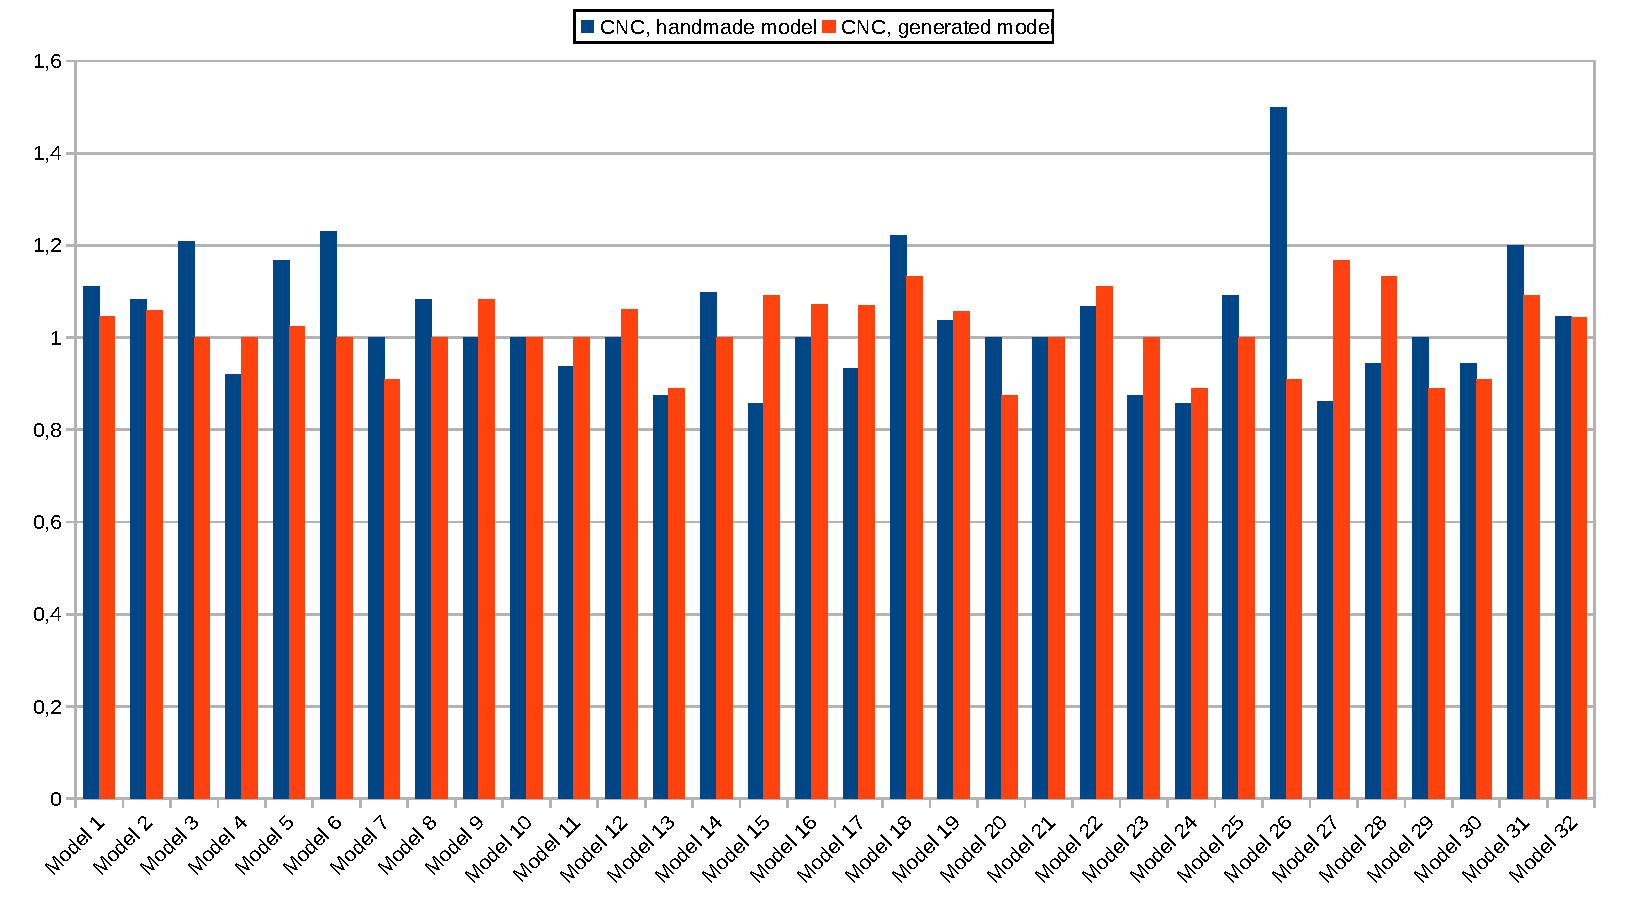
\includegraphics[width=0.95\textheight, angle=90]{./images/cnc_chart.pdf}
	\caption{Chart showing comparison of CNC metric between models}
	\label{bpmn:cnc_chart}
\end{figure}
\begin{figure}[p]
	\centering
	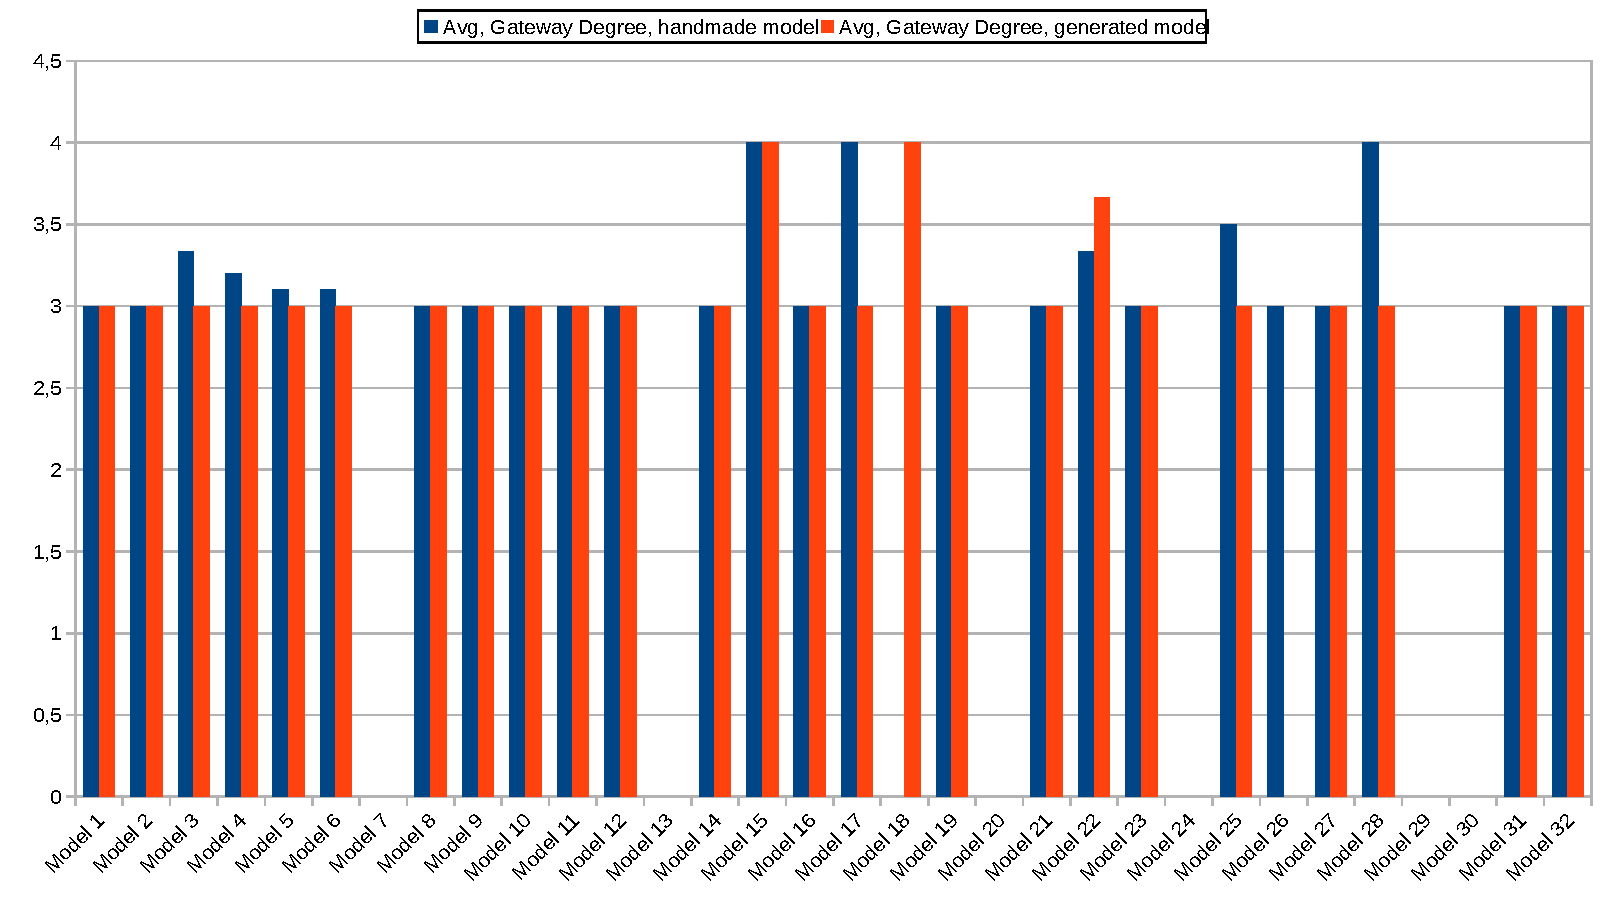
\includegraphics[width=0.95\textheight, angle=90]{./images/avg_chart.pdf}
	\caption{Chart showing comparison of Average Gateway Degree metric between models}
	\label{bpmn:avg_chart}
\end{figure}
\begin{figure}[p]
	\centering
	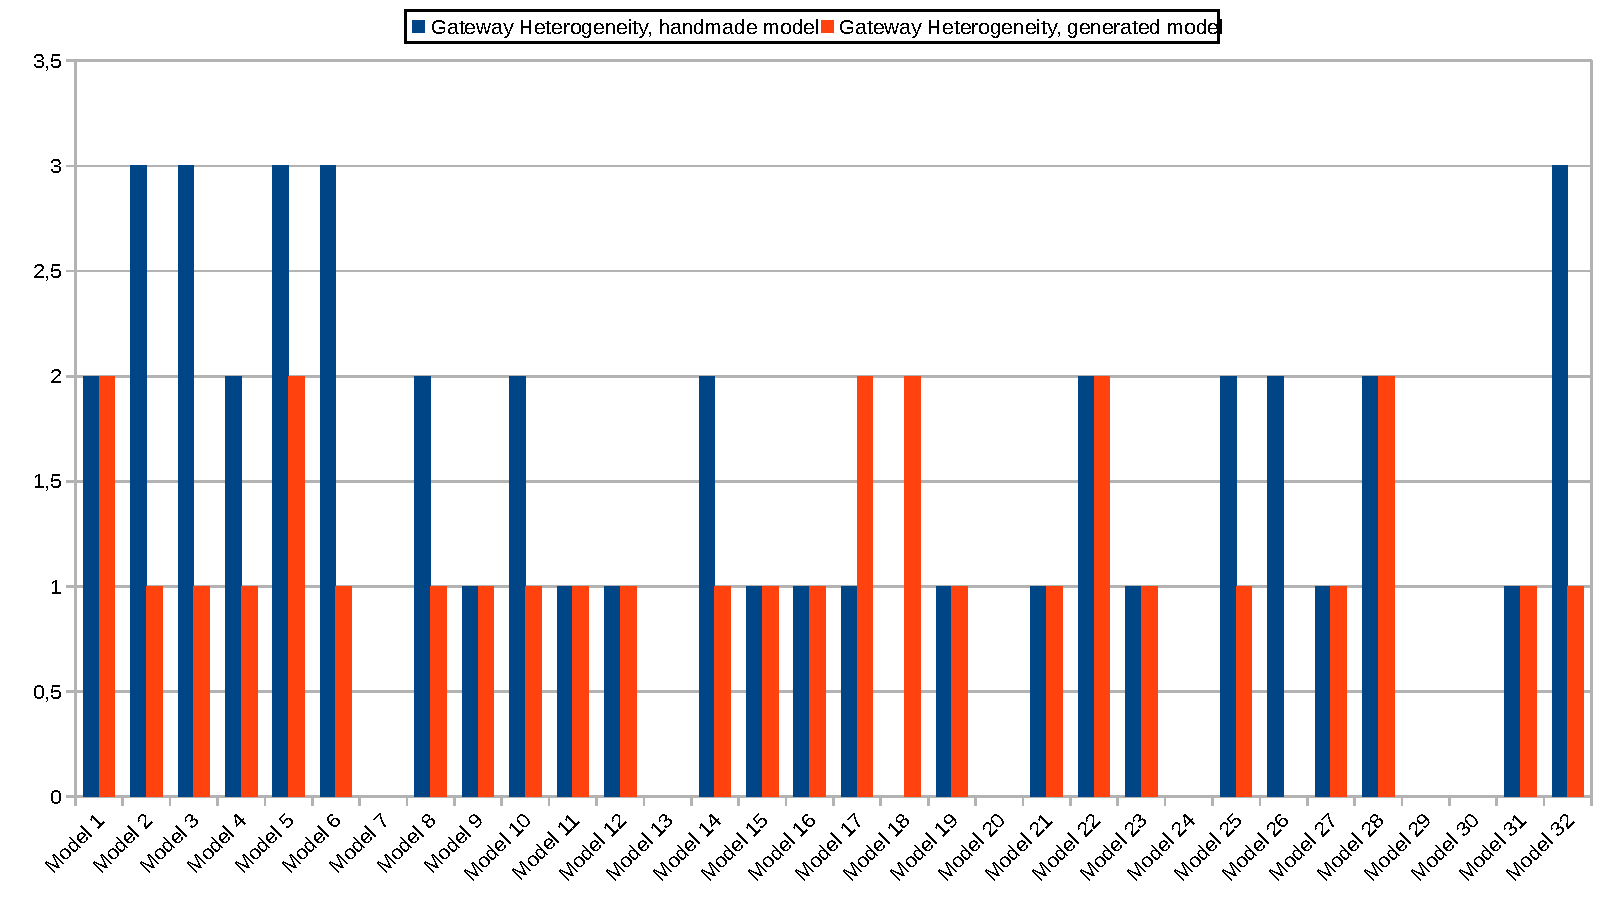
\includegraphics[width=0.95\textheight, angle=90]{./images/heter_chart.pdf}
	\caption{Chart showing comparison of Gateway Heterogeneity metric between models}
	\label{bpmn:heter_chart}
\end{figure}

\subsection{Detailed example analysis}
\label{sec:detailed-example}
In this section, a detailed analysis of a few models will be performed. This analysis will focus on generated results and the overall usability of automatically created models -- whether those capture the proper process flow from generated text and provide the useful BPMN diagrams.\\
Models number three, five and eighteen were chosen for detailed analysis. This choice of test models subset was based on the complexity metrics analysis described in previous section. Models number five and eighteen appeared a few times as a models extreme values of analysed metrics. Model number three was chosen due to the fact that its metrics values do not differentiate much from hand-made model, so it might be worthy to perform the detailed comparison and to analyse the differences that are not visible after metrics evaluation.

\subsubsection{Model 3}
\begin{tcolorbox}[
	breakable,
	arc=0mm,
	left=1pt,
	right = 1pt,
	boxrule=0mm,
	colback = {white},
	]
	\texttt{\input{./models/model3.txt}}
\end{tcolorbox}
\captionof{textdesc}{Text description for model number three}\label{txt:model3_val}
Text describes a process of taking order from guest at exclusive hotel. The described process can be separated into two parts -- registering the order by room-service manager and fulfilling it by waiter.\\
Table~\ref{csv:model3_val} shows the spreadsheet-based description of the extracted model, Figures~\ref{bpmn:generated_model3_val} and~\ref{bpmn:model3_val} present the generated BPMN diagram and corresponding hand-made model.

{\scriptsize
	\begin{longtable}{|p{0.03 \hsize}|p{0.25 \hsize}|p{0.15 \hsize}|p{0.2 \hsize}|p{0.1 \hsize}|p{0.1 \hsize}|}
		\hline
		Order & Activity & Condition & Who & Subprocess & Terminated.
		\\\hline\hline
		\csvreader[late after line=\\\hline]
		{./results/model3_intermediate_model.csv}
		{Order=\Order,Activity=\Activity,Condition=\Condition,Who=\Who,Subprocess=\Subprocess,Terminated=\Terminated}
		{\Order & \Activity & \Condition & \Who & \Subprocess & \Terminated}
		\caption{Spreadsheet-based description for process model number three}
		\label{csv:model3_val}
	\end{longtable}
}

\begin{figure}[H]
	\centering
	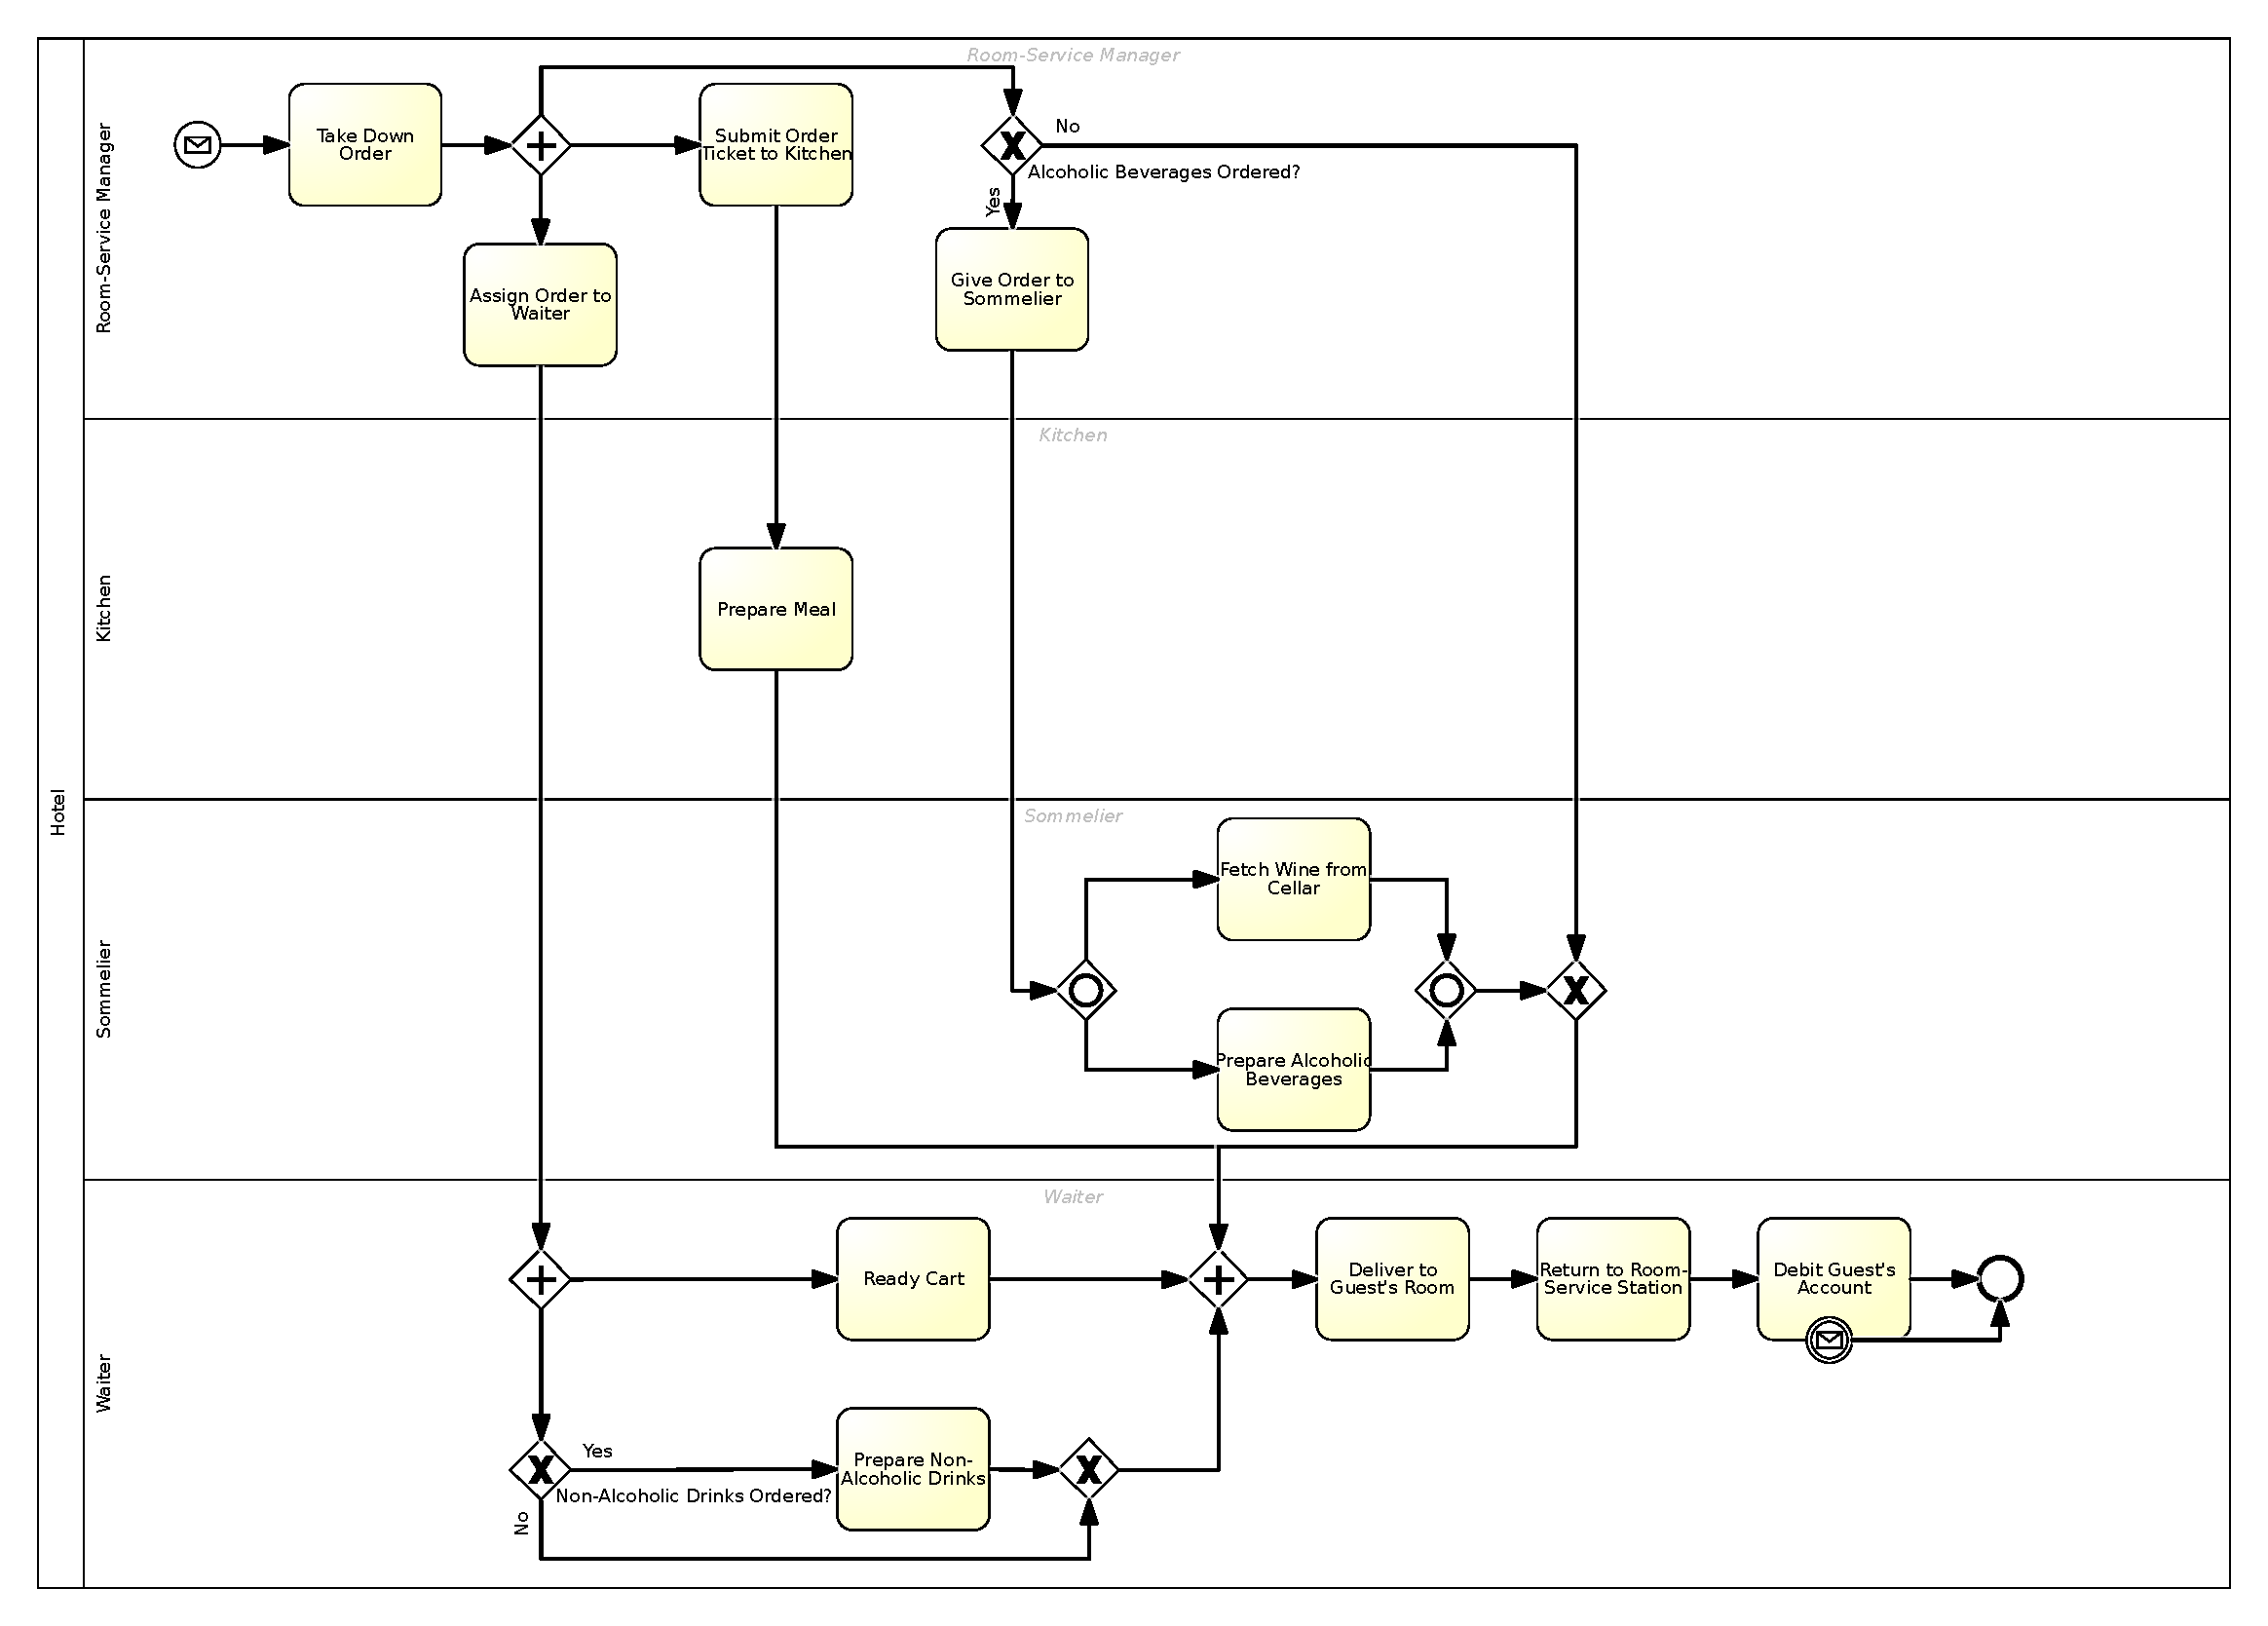
\includegraphics[width=0.95\textheight, angle=90]{./bpmn/model3.pdf}
	\caption{Hand-made BPMN diagram for process model number three}
	\label{bpmn:model3_val}
\end{figure}

\begin{figure}[H]
	\centering
	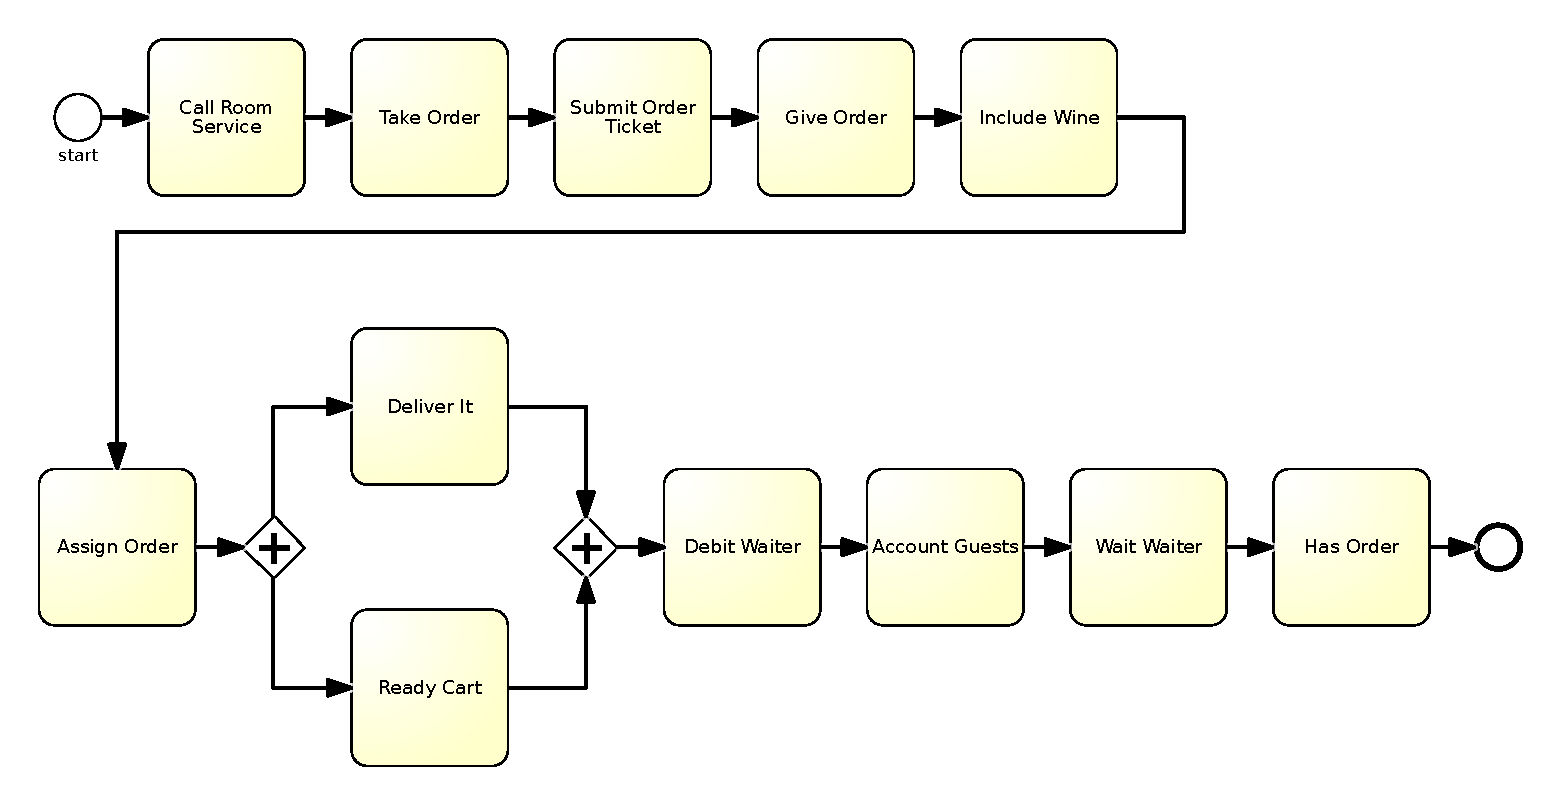
\includegraphics[width=\hsize]{./generated_bpmn/model3.pdf}
	\caption{BPMN diagram for process model number three generated from spreadsheet-based model}
	\label{bpmn:generated_model3_val}
\end{figure}

Unfortunately, the generated model is missing the pool and lanes elements, but this came from the fact, that current version of \emph{bpmn\_python} does not support the manual creation of those elements. On the other hand, the intermediate model shows that for some activities the \emph{``Who''} column was filled with correct information. In case of room-service manager the information about Participant that performs the activities is missing, due to the fact that room-service manager was addressed by a pronoun \emph{``She''}. The implemented method is unable to correctly identify actors described by pronouns and thus fails to provide correct information.\\
The first part of described process was extracted quite well -- the activities performed by room-service manager are correctly ordered. Few of the activities are missing information about the recipients of task result -- for example the activity \emph{``Submit Order Ticket''} omits the information that ticket is submitted to the kitchen.\\
The part of the process performed by waiter was more problematic. The algorithm created an incorrect parallel gateway which informs that waiter simultaneously prepares and delivers the cart, which is obviously incorrect. Several parts of description was not processed into activities -- while the part about kitchen and sommelier \emph{``doing their tasks''}, the information about waiter returning to the station was not extracted. This might be caused by the fact that verb \emph{``return''} was given in the gerund form as \emph{``returning''}. The phrase \emph{``the waiter debits the guest account''} was divided into two activities, because SpaCy parser failed to identify word \emph{``account''} as a noun and not a verb.\\
Comparing the results with hand-made model, it is apparent that latter correctly adds the activities performed by kitchen and sommelier. Also the control flow elements capture the described flow of actions in consecutive phases.

\subsubsection{Model 5}
\begin{tcolorbox}[
	breakable,
	arc=0mm,
	left=1pt,
	right = 1pt,
	boxrule=0mm,
	colback = {white},
	]
	\texttt{\input{./models/model5.txt}}
\end{tcolorbox}
\captionof{textdesc}{Text description for model number five}\label{txt:model5_val}
This process description is one of the largest from data set. The implemented method produced a process model with large number of activities involved. On the other hand, the hand-made counterpart has significantly lower number of activities, but includes higher number of control flow elements. Table~\ref{csv:model5_val} shows the spreadsheet-based description of extracted model, Figures~\ref{bpmn:generated_model5_val} and~\ref{bpmn:model5_val} presents the generated BPMN diagram and corresponding hand-made model.

{\scriptsize
	\begin{longtable}{|p{0.03 \hsize}|p{0.25 \hsize}|p{0.15 \hsize}|p{0.2 \hsize}|p{0.1 \hsize}|p{0.1 \hsize}|}
		\hline
		Order & Activity & Condition & Who & Subprocess & Terminated.
		\\\hline\hline
		\csvreader[late after line=\\\hline]
		{./results/model5_intermediate_model.csv}
		{Order=\Order,Activity=\Activity,Condition=\Condition,Who=\Who,Subprocess=\Subprocess,Terminated=\Terminated}
		{\Order & \Activity & \Condition & \Who & \Subprocess & \Terminated}
		\caption{Spreadsheet-based description for process model number five}
		\label{csv:model5_val}
	\end{longtable}
}
Comparison of the generated model with hand-made one shows that the implemented method lacks the ability to recognize some of the actions described in text as an event rather than activities. Tasks like \emph{``Create Notification''}, \emph{``Create Request''} and \emph{``Send message''} could be represented as message events. Also, the analysis of process model generated from model number five description shows that gateway extraction method fails to recognize more complex cases, which can appear in natural language. Consider the excerpt from process description, shown as Text~\ref{txt:model5_excerpt}:
\begin{tcolorbox}[
	breakable,
	arc=0mm,
	left=1pt,
	right = 1pt,
	boxrule=0mm,
	colback = {white},
	]
	\texttt{
		An electronic service then determines the significance of the customer based on information that has
		been collected during the history of the contractual relationship. In case the customer is premium, the
		process will link to an extra problem fix process (this process will not be detailed here). In case the
		customer is of certain significance which would affect the counter measures previously decided upon,
		the process goes back to re-prioritize these measures otherwise the process continues.	
	}
\end{tcolorbox}
\captionof{textdesc}{Excerpt of process description for model number five}\label{txt:model5_excerpt}
For a human modeller it is obvious that this text describes some form of conditional process flow, but it is not easy to process for machine. It might be possible to use longer phrases, like \emph{``In case of''} or \emph{``For the case that''} to signalize the possible presence of conditional flow, but there are probably a number of such phrases and identifying all of them might be a difficult task. The implemented method also had a problem with correct extraction of gateway conditions. In case of inclusive gateway added to the model, the gateway has two conditions \emph{``Problems are detected''} and \emph{``Problem is detected''}. This confusing description came from the fact, that word \emph{``no''} was labelled determiner (dependency tag ``det'') and not as a negation modifier -- thus it was omitted from condition name.

\begin{figure}[h!p]
	\centering
	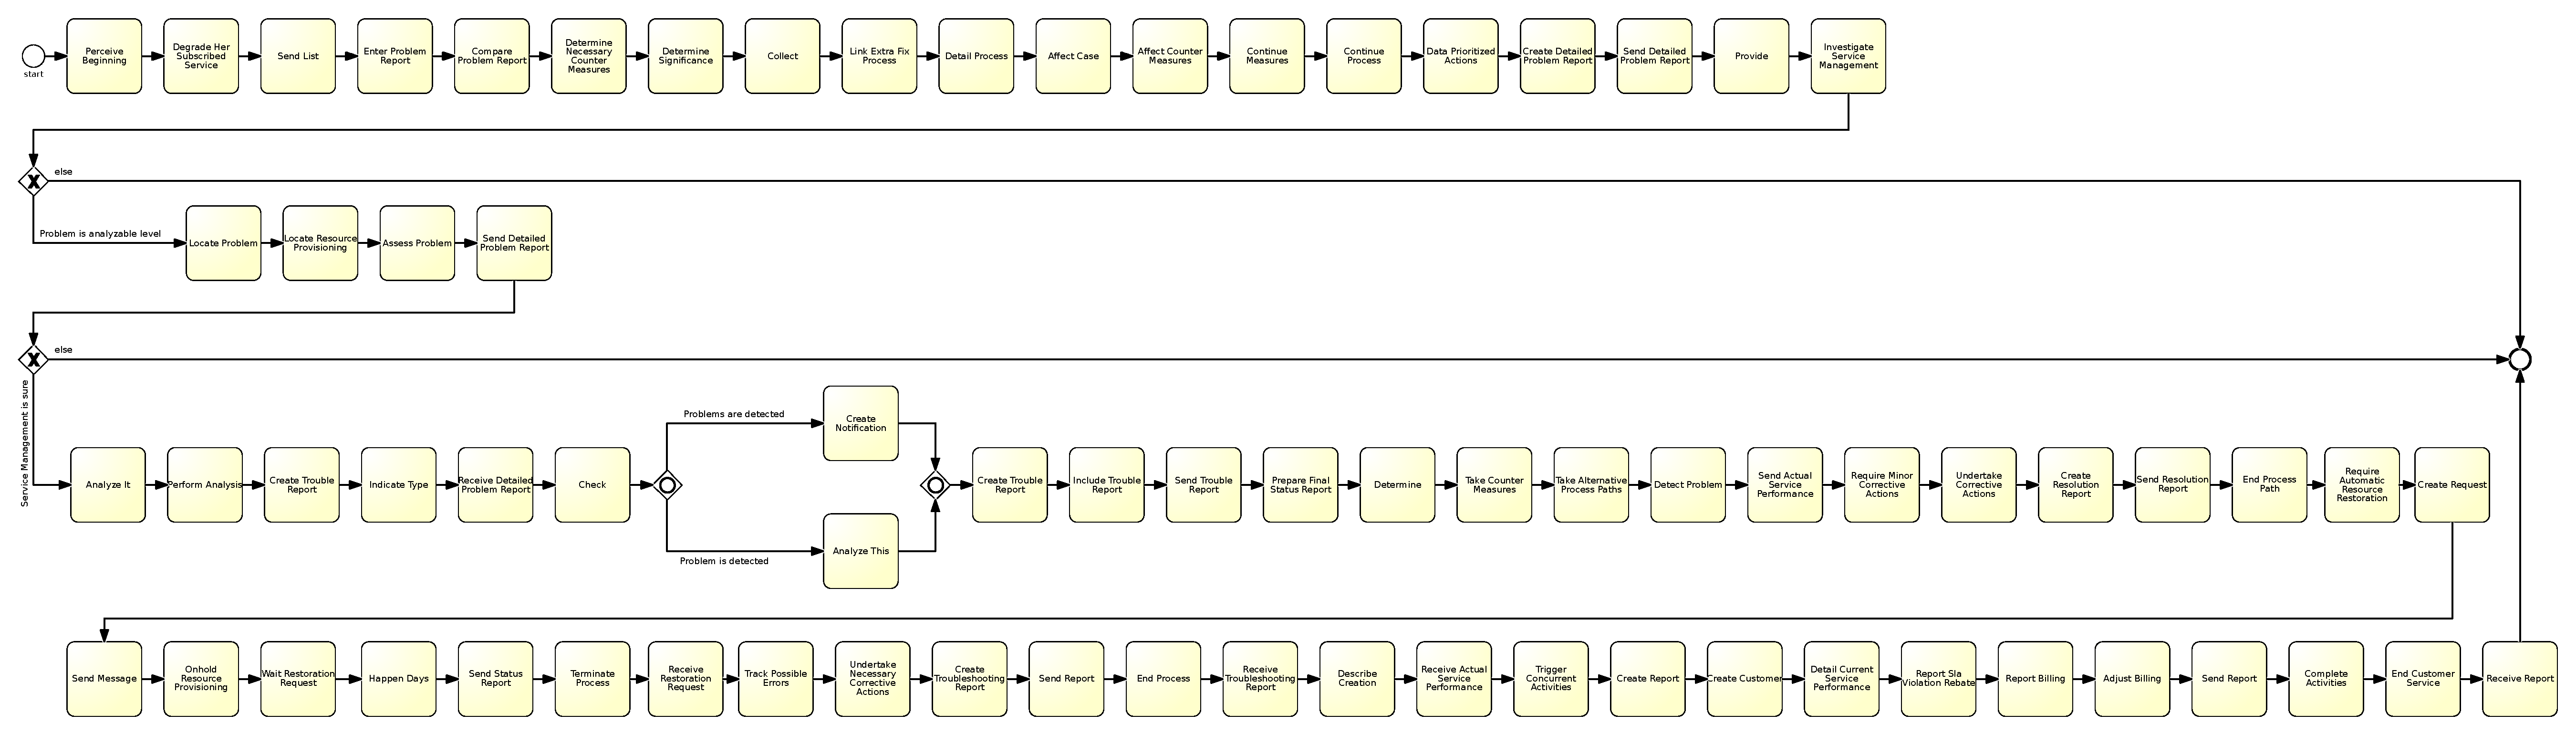
\includegraphics[width=0.90\textheight, angle=90]{./generated_bpmn/model5.pdf}
	\caption{BPMN diagram for process model number five generated from spreadsheet-based model (picture available at \url{https://github.com/KrzyHonk/nl-description-to-bpmn/tree/master/generated_bpmn})}
	\label{bpmn:generated_model5_val}
\end{figure}

\begin{figure}[h!p]
	\centering
	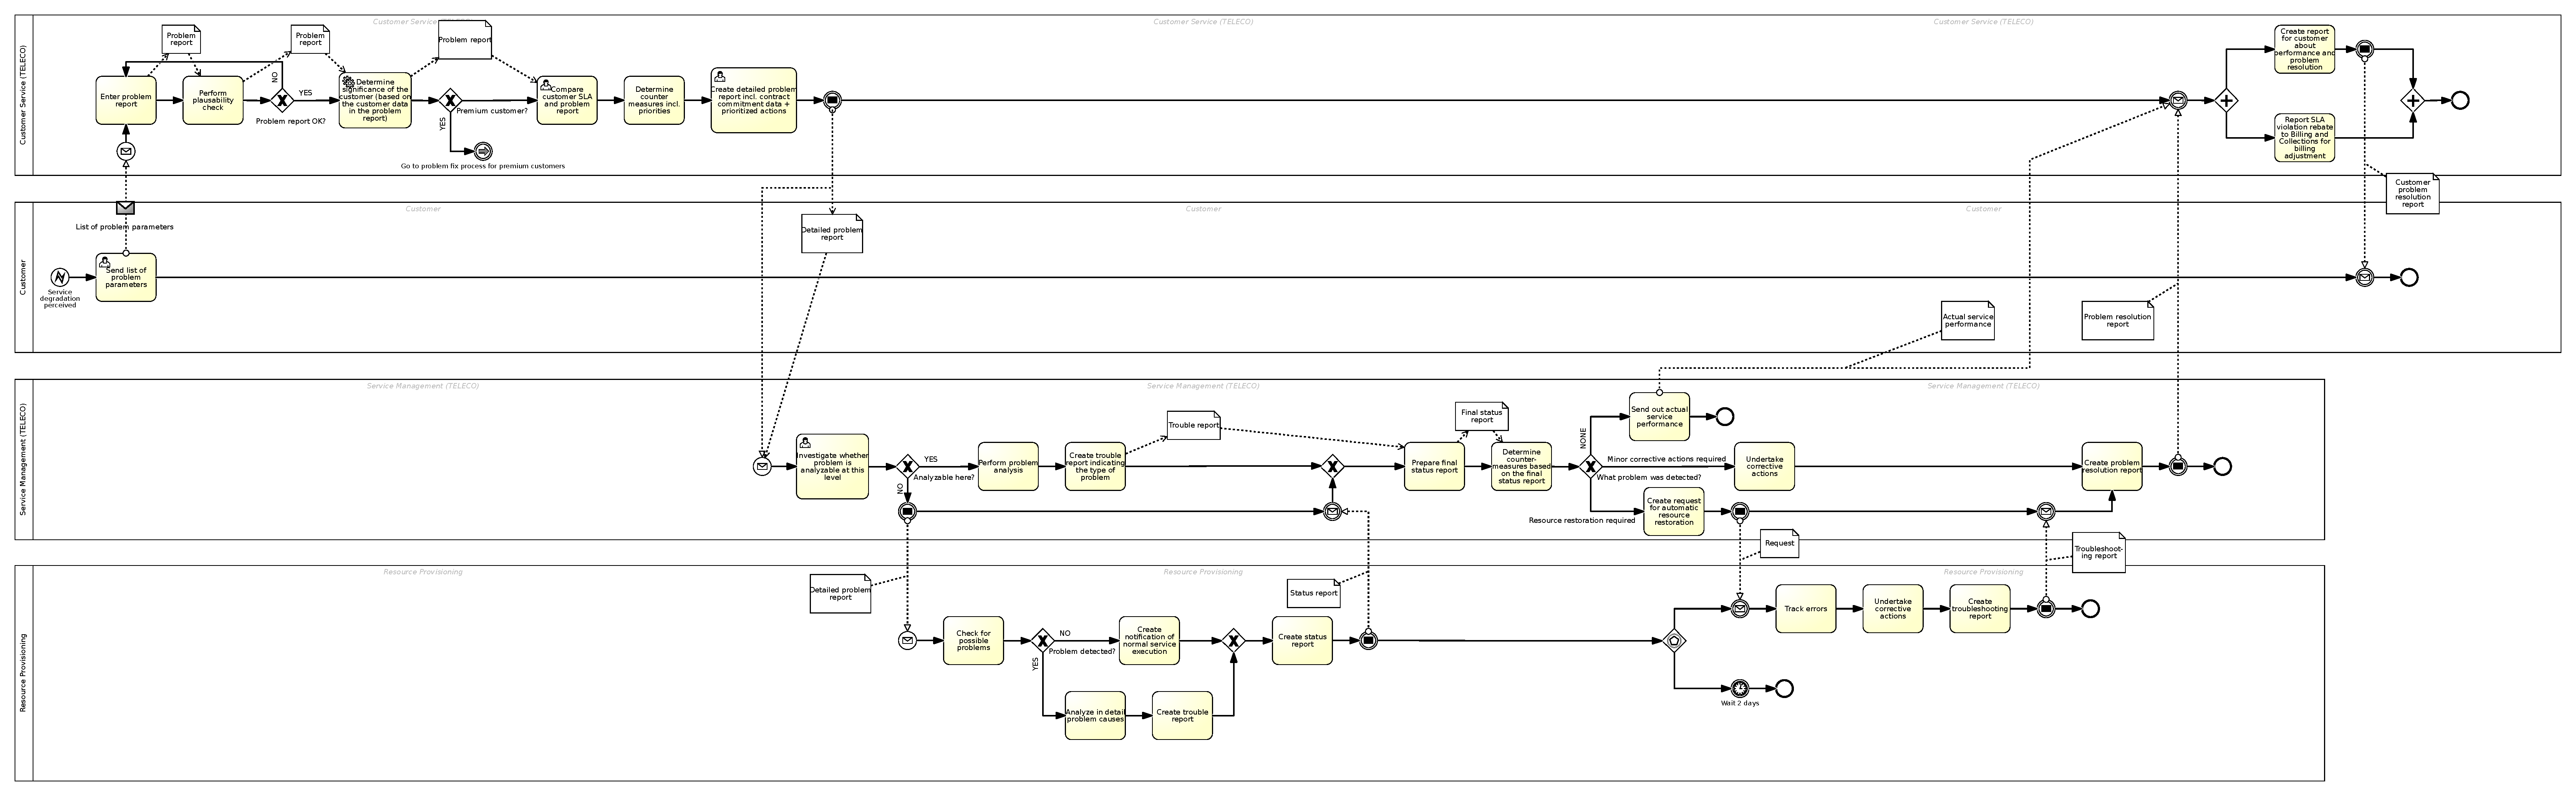
\includegraphics[width=0.90\textheight, angle=90]{./bpmn/model5.pdf}
	\caption{Hand-made BPMN diagram for process model number five (picture available at \url{https://github.com/KrzyHonk/nl-description-to-bpmn/tree/master/manual_bpmn})}
	\label{bpmn:model5_val}
\end{figure}

\subsubsection{Model 18}
\begin{tcolorbox}[
	breakable,
	arc=0mm,
	left=1pt,
	right = 1pt,
	boxrule=0mm,
	colback = {white},
	]
	\texttt{\input{./models/model18.txt}}
\end{tcolorbox}
\captionof{textdesc}{Text description for model number eighteen}\label{txt:model18_val}

{\scriptsize
	\begin{longtable}{|p{0.03 \hsize}|p{0.25 \hsize}|p{0.15 \hsize}|p{0.2 \hsize}|p{0.1 \hsize}|p{0.1 \hsize}|}
		\hline
		Order & Activity & Condition & Who & Subprocess & Terminated.
		\\\hline\hline
		\csvreader[late after line=\\\hline]
		{./results/model18_intermediate_model.csv}
		{Order=\Order,Activity=\Activity,Condition=\Condition,Who=\Who,Subprocess=\Subprocess,Terminated=\Terminated}
		{\Order & \Activity & \Condition & \Who & \Subprocess & \Terminated}
		\caption{Spreadsheet-based description for process model number eighteen}
		\label{csv:model18_val}
	\end{longtable}
}

\begin{figure}[h!p]
\centering
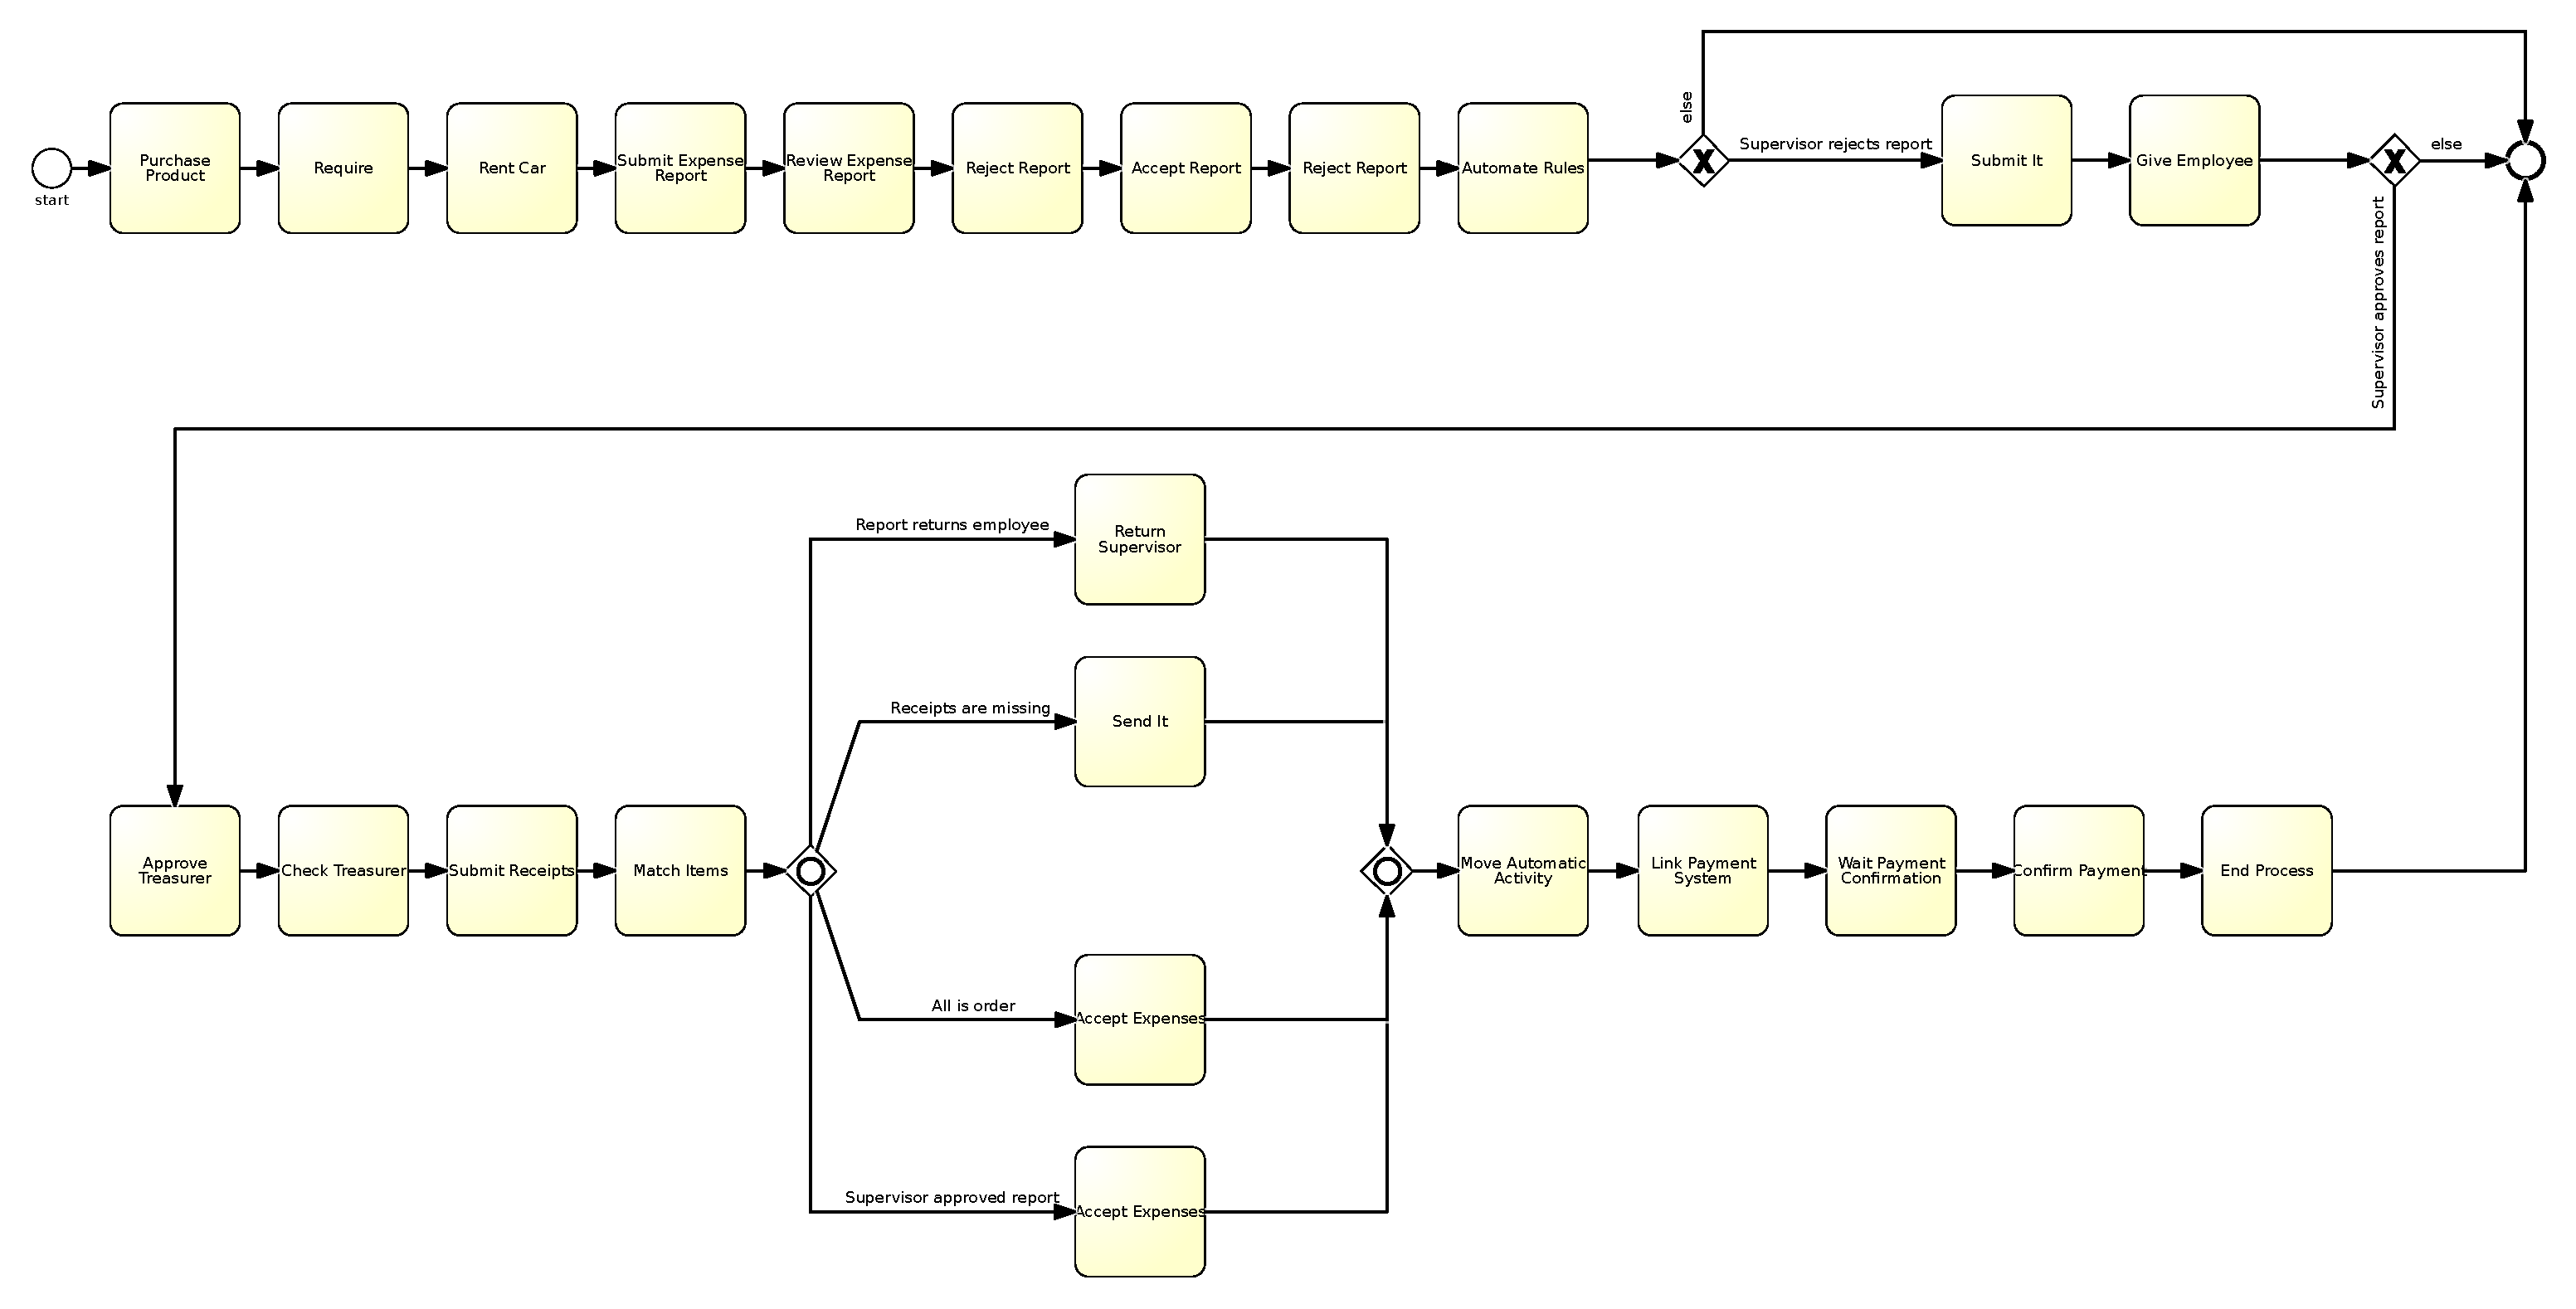
\includegraphics[width=\hsize]{./generated_bpmn/model18.pdf}
\caption{BPMN diagram for process model number eighteen generated from spreadsheet-based model}
\label{bpmn:generated_model18_val}
\end{figure}

\begin{figure}[h!p]
	\centering
	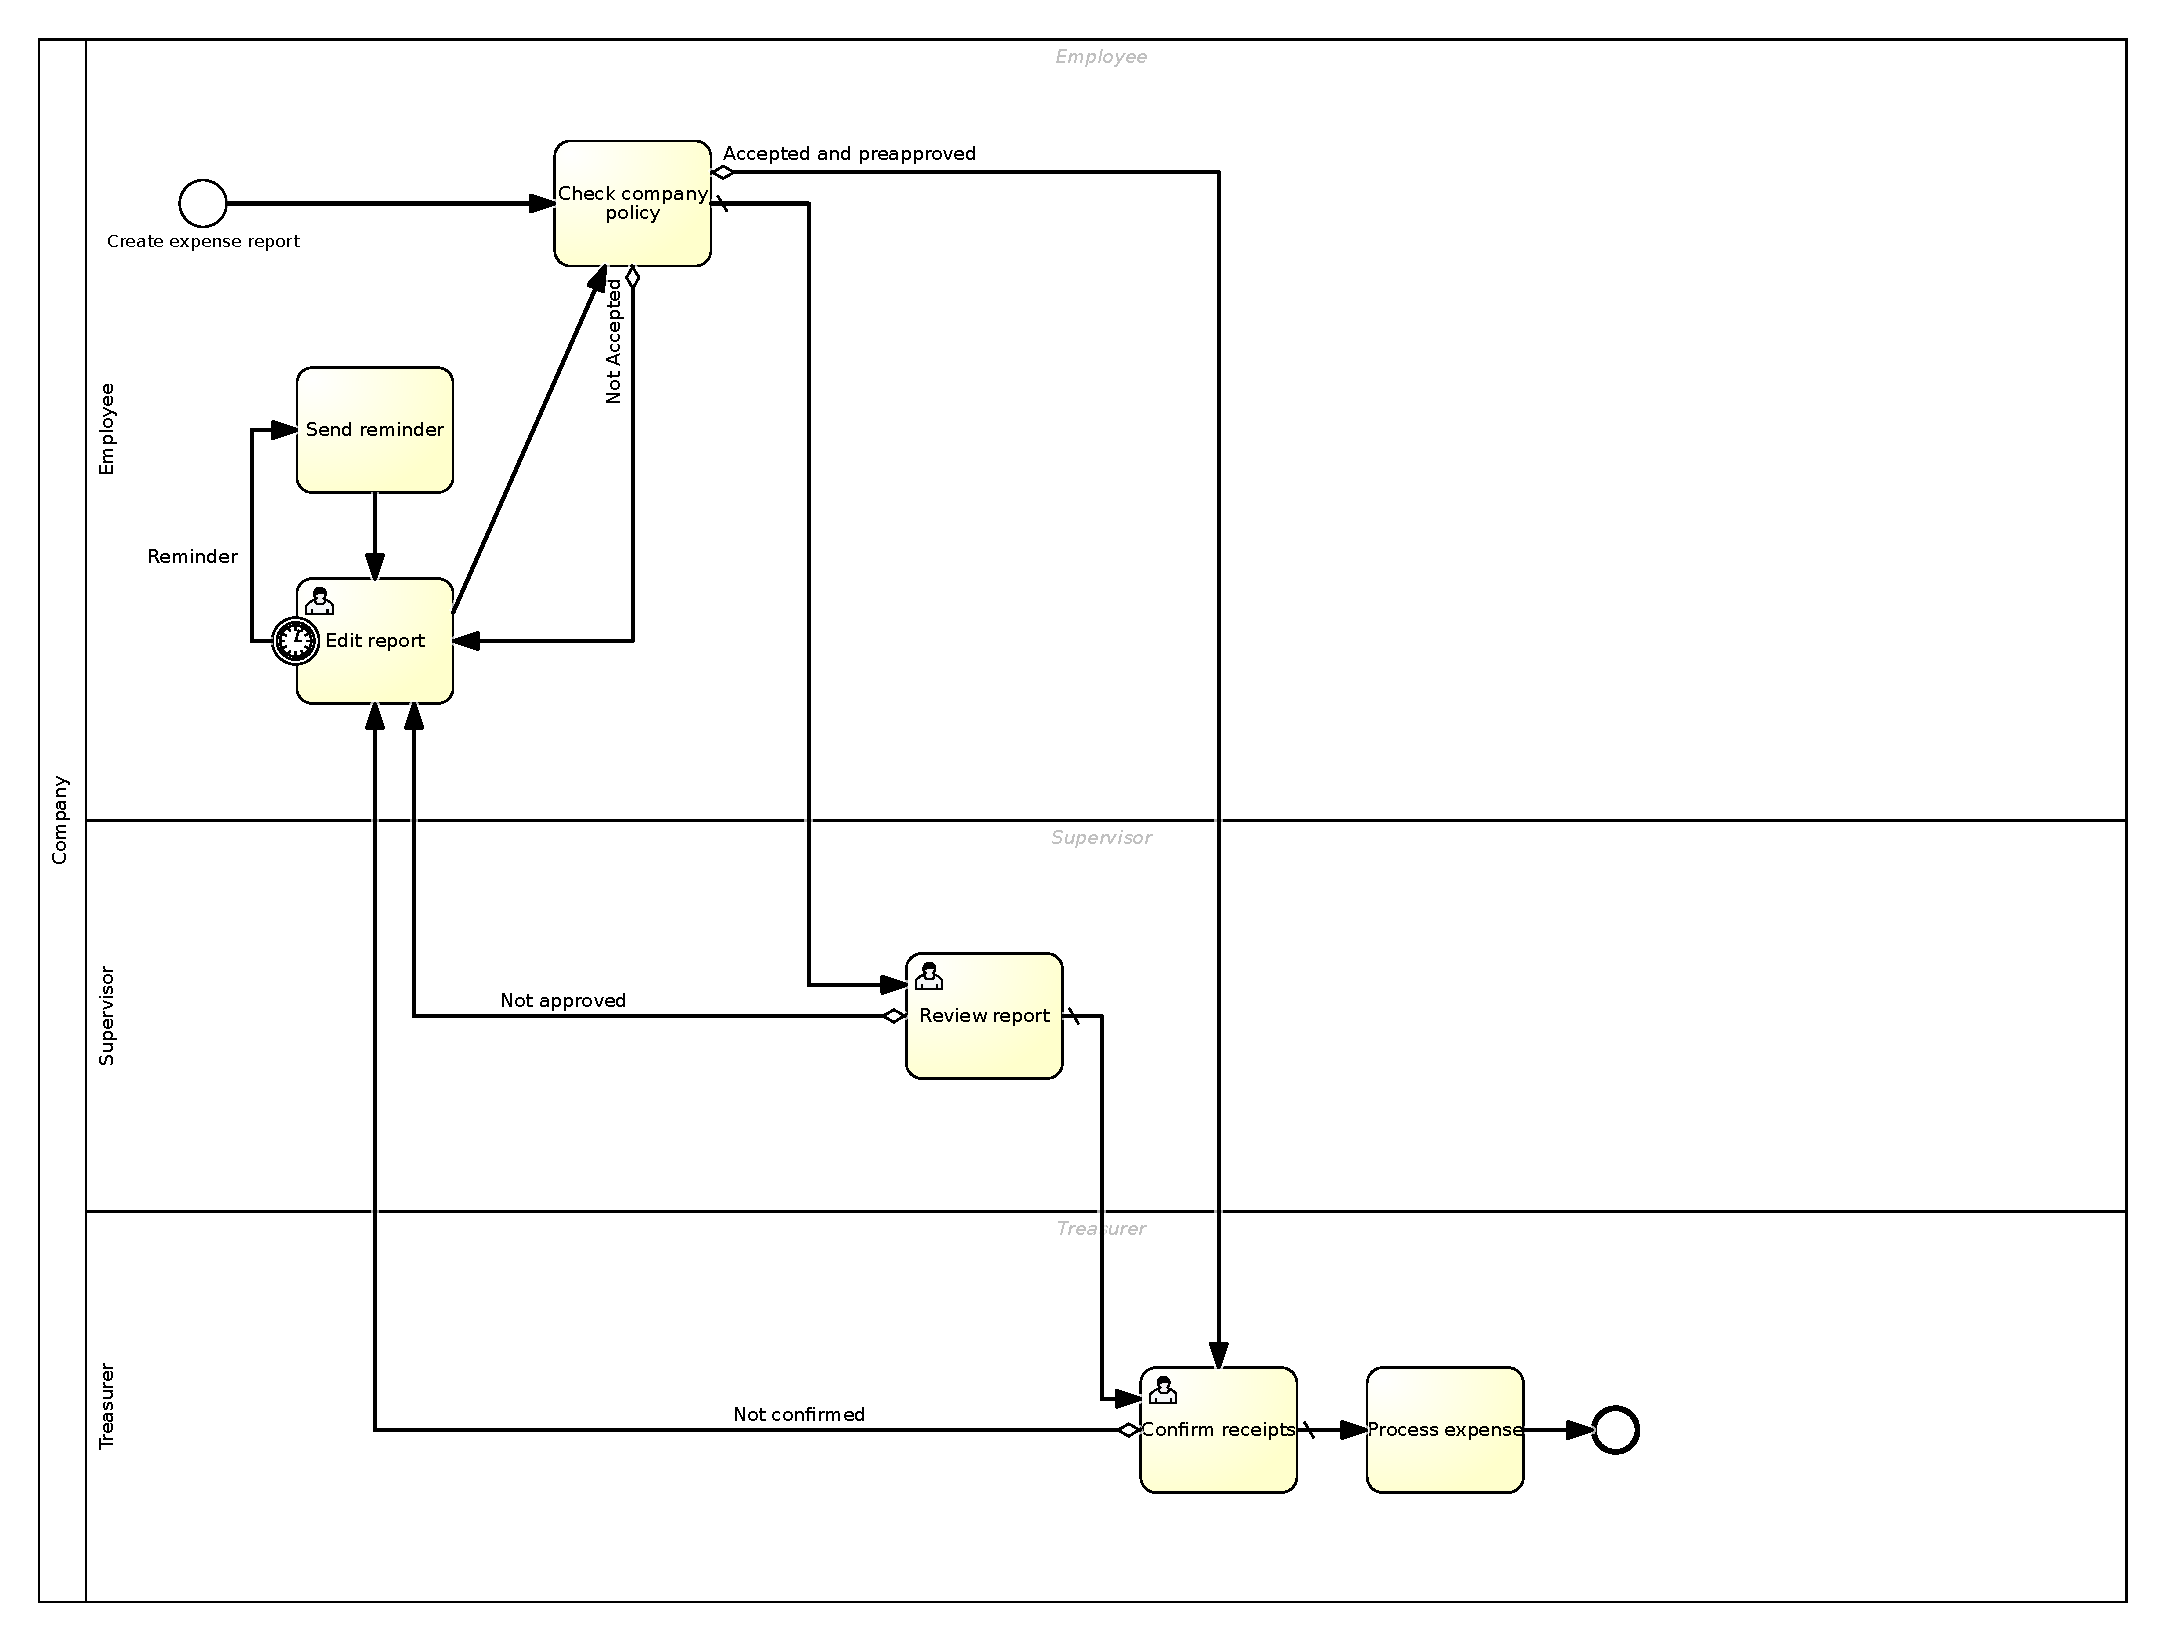
\includegraphics[width=\hsize]{./bpmn/model18.pdf}
	\caption{Hand-made BPMN diagram for process model number eighteen}
	\label{bpmn:model18_val}
\end{figure}

Like in the previous case, the model generated from this description has higher number of the activities, compared to the hand-made model. In this case, the reason is the fact that process description includes parts that do not describe an activities involved in the process, but rather add some additional information about process itself. Consider those parts shown as Texts~\ref{txt:model18_excerpt_one} and~\ref{txt:model18_excerpt_two}:
\begin{tcolorbox}[
	breakable,
	arc=0mm,
	left=1pt,
	right = 1pt,
	boxrule=0mm,
	colback = {white},
	]
	\texttt{
		An employee purchases a product or service he requires. For instance, a sales person on
		a trip rents a car.	
	}
\end{tcolorbox}
\captionof{textdesc}{First excerpt of process description for model number eighteen}\label{txt:model18_excerpt_one}
\begin{tcolorbox}[
	breakable,
	arc=0mm,
	left=1pt,
	right = 1pt,
	boxrule=0mm,
	colback = {white},
	]
	\texttt{
		Since the company has expense rules, there are circumstances where
		the supervisor can accept or reject the report upon first inspection. These rules could be
		automated, to reduce the workload on the supervisor.	
	}
\end{tcolorbox}
\captionof{textdesc}{Second excerpt of process description for model number eighteen}\label{txt:model18_excerpt_two}
The first excerpt provides an introduction for the described process case, the second excerpt gives an insight to the way in which the described company works. Both excerpts do not describe the actual process flow and while it is easy to recognize this for a human, a machine translation algorithm does not have the knowledge required to identify such cases. The presented method simply processes such information and create unnecessary activities (\emph{``Rent Car''}, \emph{``Automate Rules'}) from those excerpts. Overcoming this obstacle might be a challenging task.

\section{Method limitations}
The evaluation of implemented method of generating business process model from natural language description pointed out a number of limitations of implemented prototype. The most important of those limitations are:
\begin{itemize}
	\item adding only tasks and gateways to resulting model -- in some cases adding an intermediate event instead of the task might provide a better representation of a described process. The simplest way to solve this problem might be to add additional layer of SVO validation, which would check the verb included in SVO against a set of designated keywords. Examples of such keywords might be \emph{``send''} or \emph{``report''} (if identified as a verb) -- if SVO consists such a verb, it might be better to represent it as an intermediate message event, rather than a task,
	\item the proposed method for gateway extraction is unable to recognize more complex cases of conditional flow -- those can be signalized by specific phrases, such as \emph{``In case of''}, \emph{``For the case that''} and others,
	\item if the description consists some information that are not a part of process flow, it will be also incorporated into the created BPMN. While this problem might be impossible to overcome by improving the algorithm (machine do not understand the context of processed text), it might be a good idea to incorporate a lightweight standardization to the text and require that description covers only information about process flow,
	\item identifying the actual actors in the process, that were addressed by pronoun word (\emph{``I''}, \emph{``He''}, \emph{``She''}). This is a problem known as a anaphora resolution, and it is already covered in multiple sources~(\cite{anaphora-hale},~\cite{anaphora-kotek}). Implementing a solution for anaphora resolution might improve results of process generation -- with this, it might be possible to identify an actor for every activity in a process and enhance the generated model with pools and lanes.
\end{itemize}
This section described the validation methodology applied to implemented prototype and presented the validation results. Also, the proposed methodology limitations were highlighted. Next section summarises the proposed approach and concludes this work.
\chapter{Conclusion}
\label{cha:conclusion}
\section{Summary}
In this thesis, a solution for the problem of automatic generation of business process models from natural language description was presented. An effective, machine-aided transformation from a semi-formal or informal document into a process model might be more time-efficient in comparison to the manual generation of process model diagram. In addition, maintenance of formal process models and documentation might become easier, especially for people, who do not have the sufficient knowledge and expertise in process modelling field.\\
The proposed solution is based on syntactic analysis of business process description and extracting Subject-Verb-Object constructs (SVO), which can be later transformed into process elements. The presented method is enhanced with semantic analysis of the text, which allows to filter out unnecessary SVO constructs. The methodology presented in this thesis is divided the following steps:
\begin{enumerate}
	\item Participants extraction -- a sentence from a given description is analysed, and the information about possible participants in process are extracted,
	\item Subject-verb-object constructs extraction -- a sentence from given description is analysed in search of basic SVO constructs,
	\item Gateway keywords search -- a process description is analysed in search of the keywords that signalizes the presence of logical gateways,
	\item Intermediate process model generation -- an intermediate process model is created from the acquired data,
	\item BPMN diagram generation -- a BPMN diagram is generated from the intermediate process model.
\end{enumerate}
A prototype of the proposed method was implemented using Python programming language and SpaCy library, which provides many useful Natural Language Processing tools (syntax parser, WordNet lexical database API). This prototype was tested against a test set of natural language business process descriptions, gathered from a few academic sources. The validation of test results shows that proposed method is able to create a complete process model, but a few limitations of presented approach were highlighted (only task and gateway elements used in generated models, limited effectiveness of gateway extraction, problems with extracting invalid activities from description, lack of anaphora resolution).

\section{Conclusion. Further works}
The proposed method of generating process model from natural language description provides some basic information about the described process in the form of BPMN diagram. It is not able to extract more complex constructs and is only able to handle basic elements of BPMN standard. Dealing with the method limitations listed in the previous section provides a direction for further work on improving the proposed solution. Enhancing the process models, generated using proposed method, with additional BPMN elements (such as intermediate events, pools and lanes); extractions more information about conditional flows and gateways; adding anaphora resolution to identify real actors in process -- these improvements are possible to achieve with further work on proposed method.\\
On the other hand, extracting business process information from natural language description proved to be a difficult task. The problem lies in the nature of natural language -- the natural language processing methods have a limited knowledge of semantics and context of words. It is almost impossible to discard these parts of description, which do not provide any information about process execution. Thus, it might be a better idea to implement a semi-automatic solution, which requires some amount of human aid or to abandon natural language description for some sort of standardized format or structured natural language description. For example, there are a few publications that focus on the subject of translating the SBVR notation into process models~\cite{sbvr-automat}. By using the SBVR as a process description format it is possible to define basic syntax and structure for description, which can be easier to process.\\
Nevertheless, generating a process model from natural language description is a challenging task. The proposed method provides limited results, but with further development, it might be possible to provide overcome the highlighted problems and improve the results significantly.

\bibliography{bibliografia}

\appendix
\chapter{Detailed results}
\label{cha:detailed-results}
\section{Model 1}
\begin{tcolorbox}[
	breakable,
	arc=0mm,
	left=1pt,
	right = 1pt,
	boxrule=0mm,
	colback = {white},
	]
	\texttt{\input{./models/model1.txt}}
\end{tcolorbox}
\captionof{textdesc}{Text description for model 1}
\label{txt:model1}

{\scriptsize
	\begin{longtable}{|p{0.03 \hsize}|p{0.25 \hsize}|p{0.15 \hsize}|p{0.2 \hsize}|p{0.1 \hsize}|p{0.1 \hsize}|}
		\hline
		Order & Activity & Condition & Who & Subprocess & Terminated.
		\\\hline\hline
		\csvreader[late after line=\\\hline]
		{./results/model1_intermediate_model.csv}
		{Order=\Order,Activity=\Activity,Condition=\Condition,Who=\Who,Subprocess=\Subprocess,Terminated=\Terminated}
		{\Order & \Activity & \Condition & \Who & \Subprocess & \Terminated}
		\caption{Spreadsheet-based description for process model 1}
		\label{csv:model1}
	\end{longtable}
}

\begin{figure}[H]
	\centering
	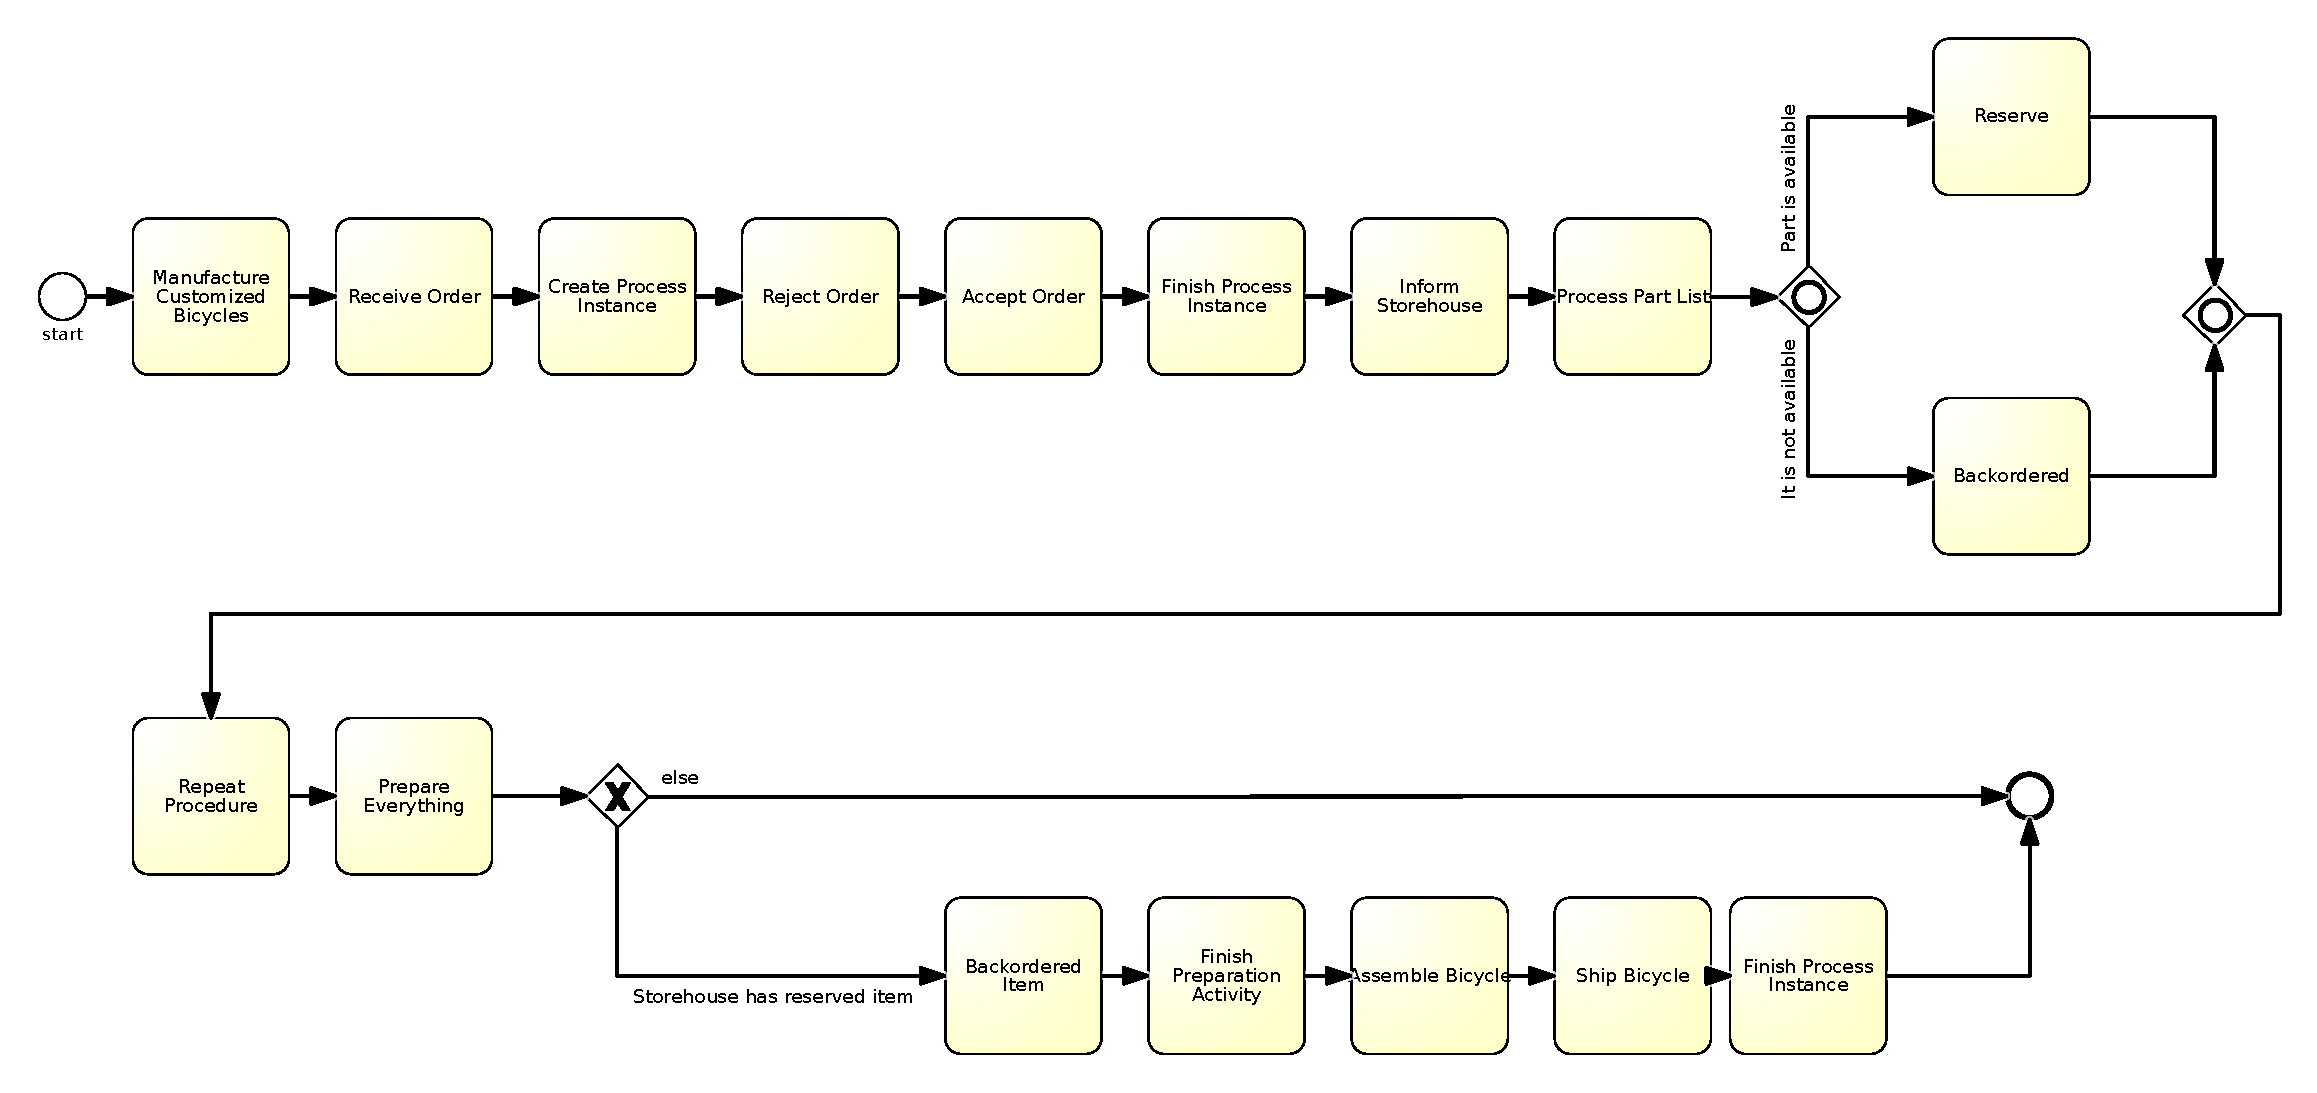
\includegraphics[width=\hsize]{./generated_bpmn/model1.pdf}
	\caption{BPMN diagram for process model 1 generated from spreadsheet-based model}
	\label{bpmn:generated_model1}
\end{figure}

\begin{figure}[H]
	\centering
	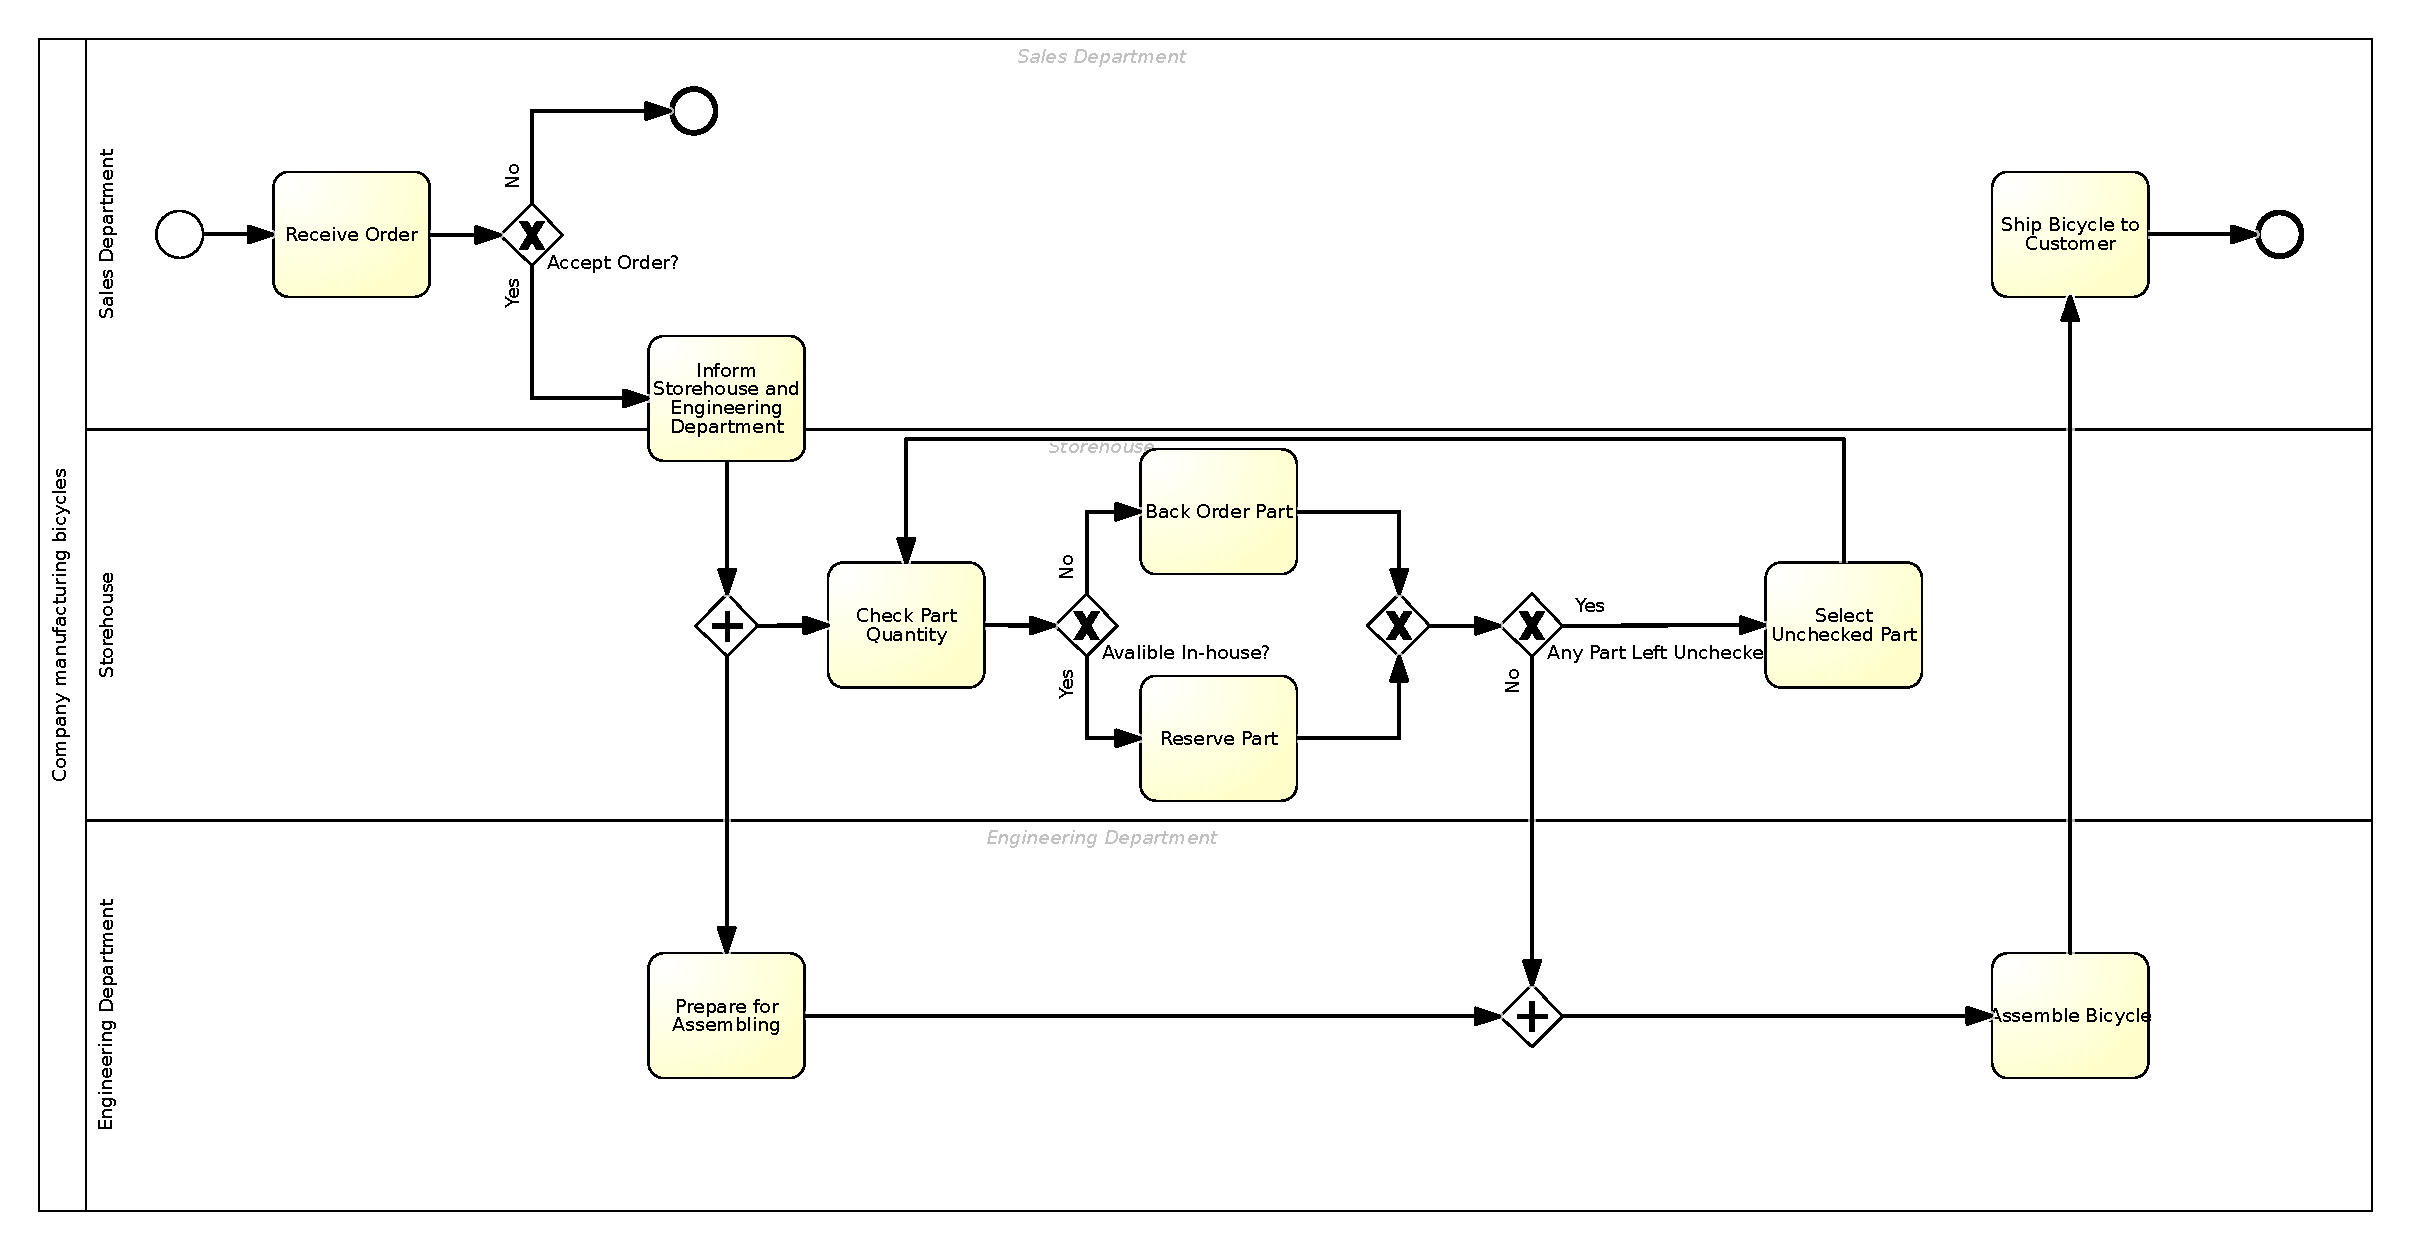
\includegraphics[width=\hsize]{./bpmn/model1.pdf}
	\caption{Hand-made BPMN diagram for process model 1}
	\label{bpmn:model1}
\end{figure}

\section{Model 2}
\begin{tcolorbox}[
	breakable,
	arc=0mm,
	left=1pt,
	right = 1pt,
	boxrule=0mm,
	colback = {white},
	]
	\texttt{\input{./models/model2.txt}}
\end{tcolorbox}
\captionof{textdesc}{Text description for model 2}
\label{txt:model2}

{\scriptsize
	\begin{longtable}{|p{0.03 \hsize}|p{0.25 \hsize}|p{0.15 \hsize}|p{0.2 \hsize}|p{0.1 \hsize}|p{0.1 \hsize}|}
		\hline
		Order & Activity & Condition & Who & Subprocess & Terminated.
		\\\hline\hline
		\csvreader[late after line=\\\hline]
		{./results/model2_intermediate_model.csv}
		{Order=\Order,Activity=\Activity,Condition=\Condition,Who=\Who,Subprocess=\Subprocess,Terminated=\Terminated}
		{\Order & \Activity & \Condition & \Who & \Subprocess & \Terminated}
		\caption{Spreadsheet-based description for process model 2}
		\label{csv:model2}
	\end{longtable}
}

\begin{figure}[H]
	\centering
	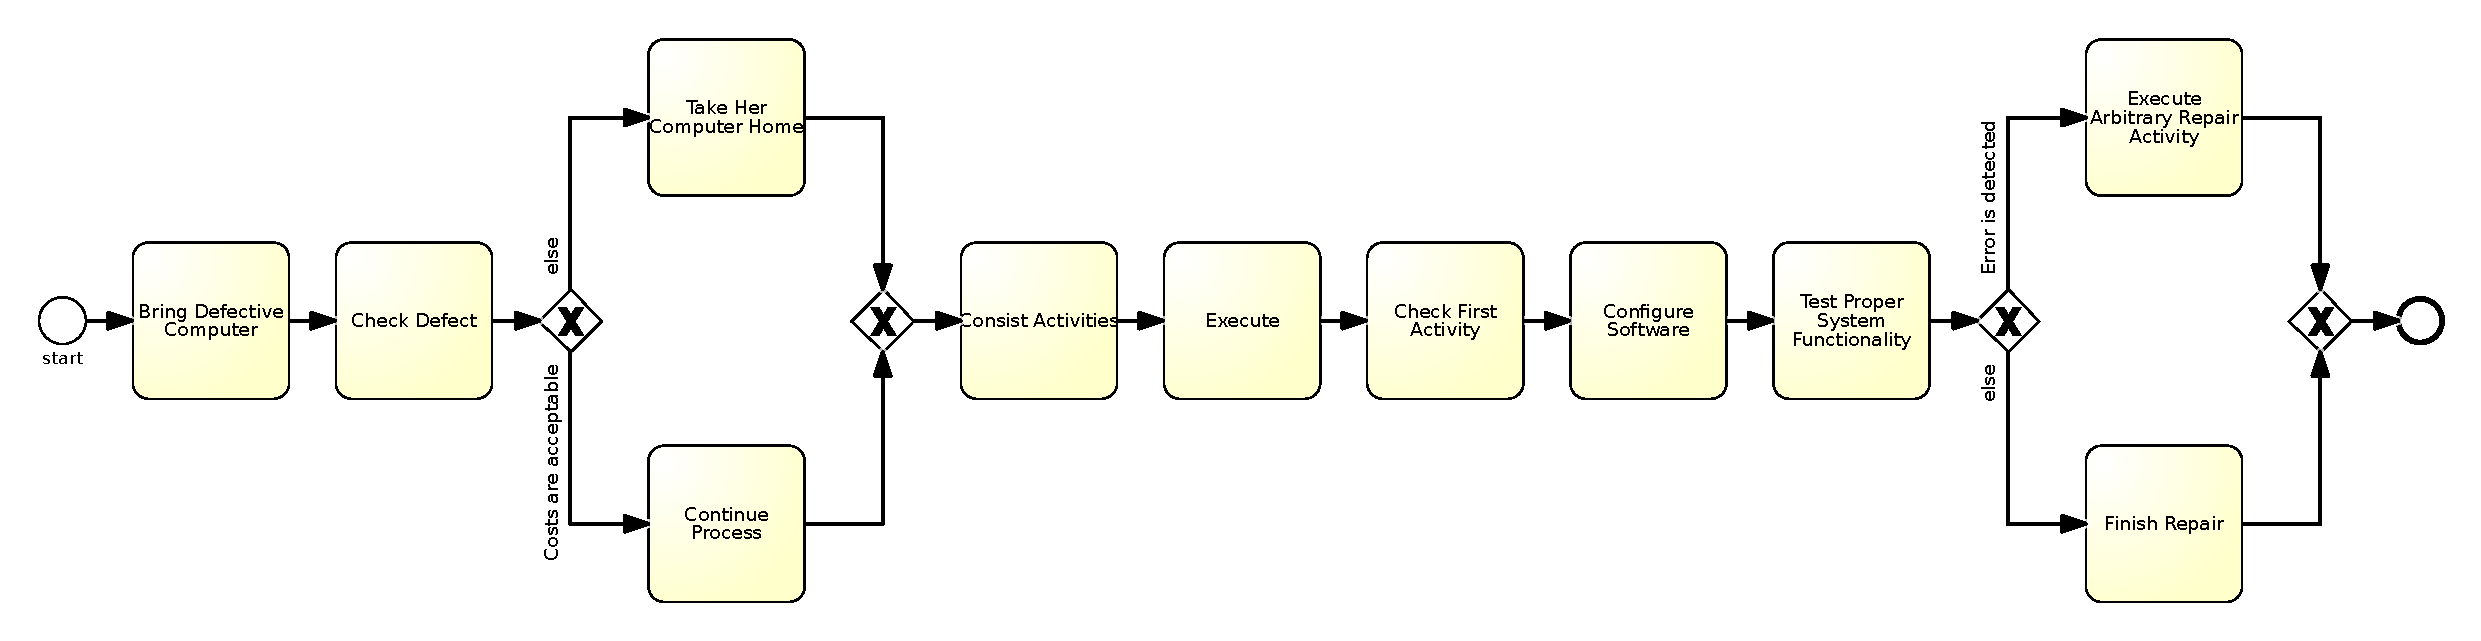
\includegraphics[width=\hsize]{./generated_bpmn/model2.pdf}
	\caption{BPMN diagram for process model 2 generated from spreadsheet-based model}
	\label{bpmn:generated_model2}
\end{figure}

\begin{figure}[H]
	\centering
	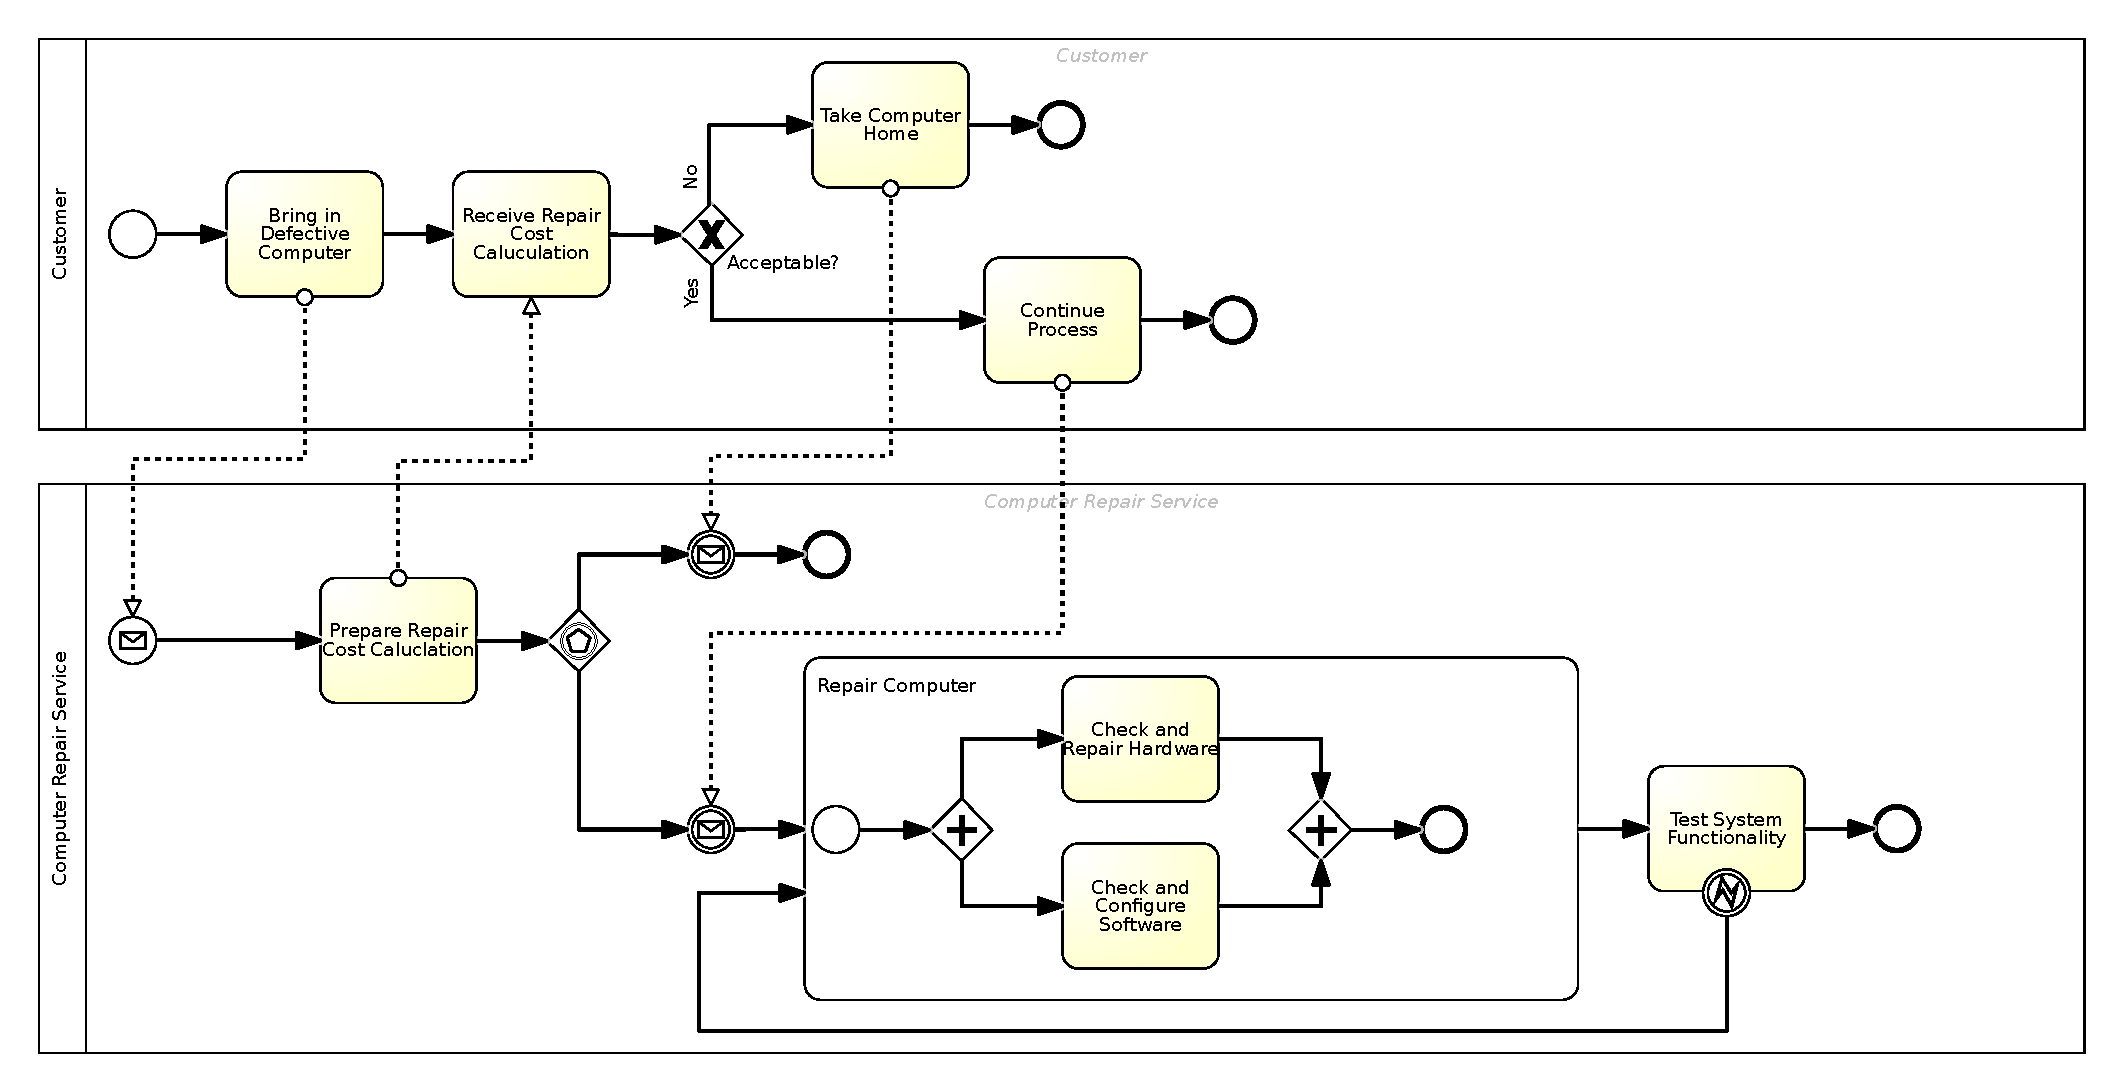
\includegraphics[width=\hsize]{./bpmn/model2.pdf}
	\caption{Hand-made BPMN diagram for process model 2}
	\label{bpmn:model2}
\end{figure}

\section{Model 3}
\begin{tcolorbox}[
	breakable,
	arc=0mm,
	left=1pt,
	right = 1pt,
	boxrule=0mm,
	colback = {white},
	]
	\texttt{\input{./models/model3.txt}}
\end{tcolorbox}
\captionof{textdesc}{Text description for model 3}
\label{txt:model3}

{\scriptsize
	\begin{longtable}{|p{0.03 \hsize}|p{0.25 \hsize}|p{0.15 \hsize}|p{0.2 \hsize}|p{0.1 \hsize}|p{0.1 \hsize}|}
		\hline
		Order & Activity & Condition & Who & Subprocess & Terminated.
		\\\hline\hline
		\csvreader[late after line=\\\hline]
		{./results/model3_intermediate_model.csv}
		{Order=\Order,Activity=\Activity,Condition=\Condition,Who=\Who,Subprocess=\Subprocess,Terminated=\Terminated}
		{\Order & \Activity & \Condition & \Who & \Subprocess & \Terminated}
		\caption{Spreadsheet-based description for process model 3}
		\label{csv:model3}
	\end{longtable}
}

\begin{figure}[H]
	\centering
	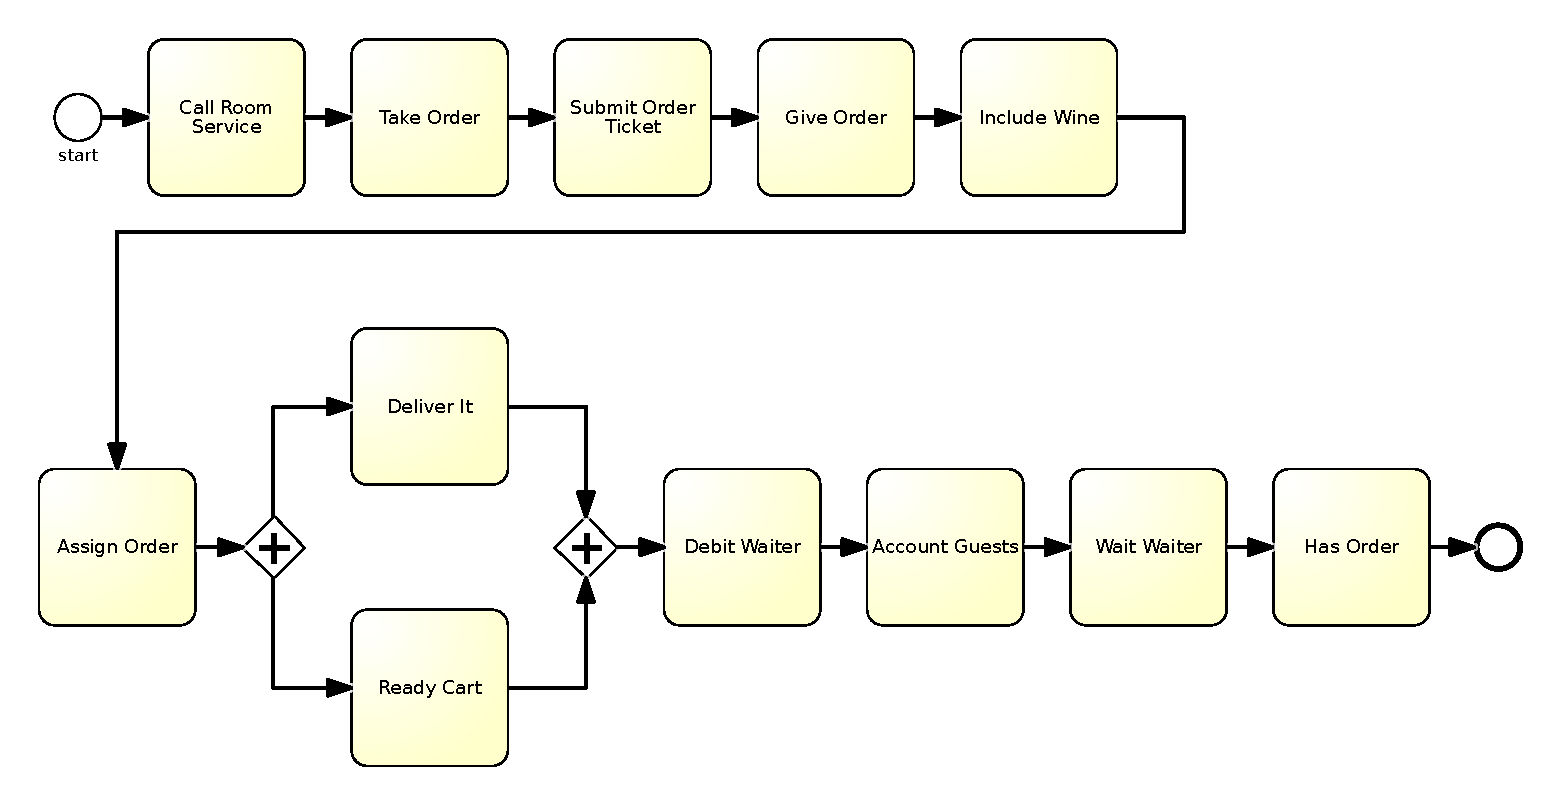
\includegraphics[width=\hsize]{./generated_bpmn/model3.pdf}
	\caption{BPMN diagram for process model 3 generated from spreadsheet-based model}
	\label{bpmn:generated_model3}
\end{figure}

\begin{figure}[H]
	\centering
	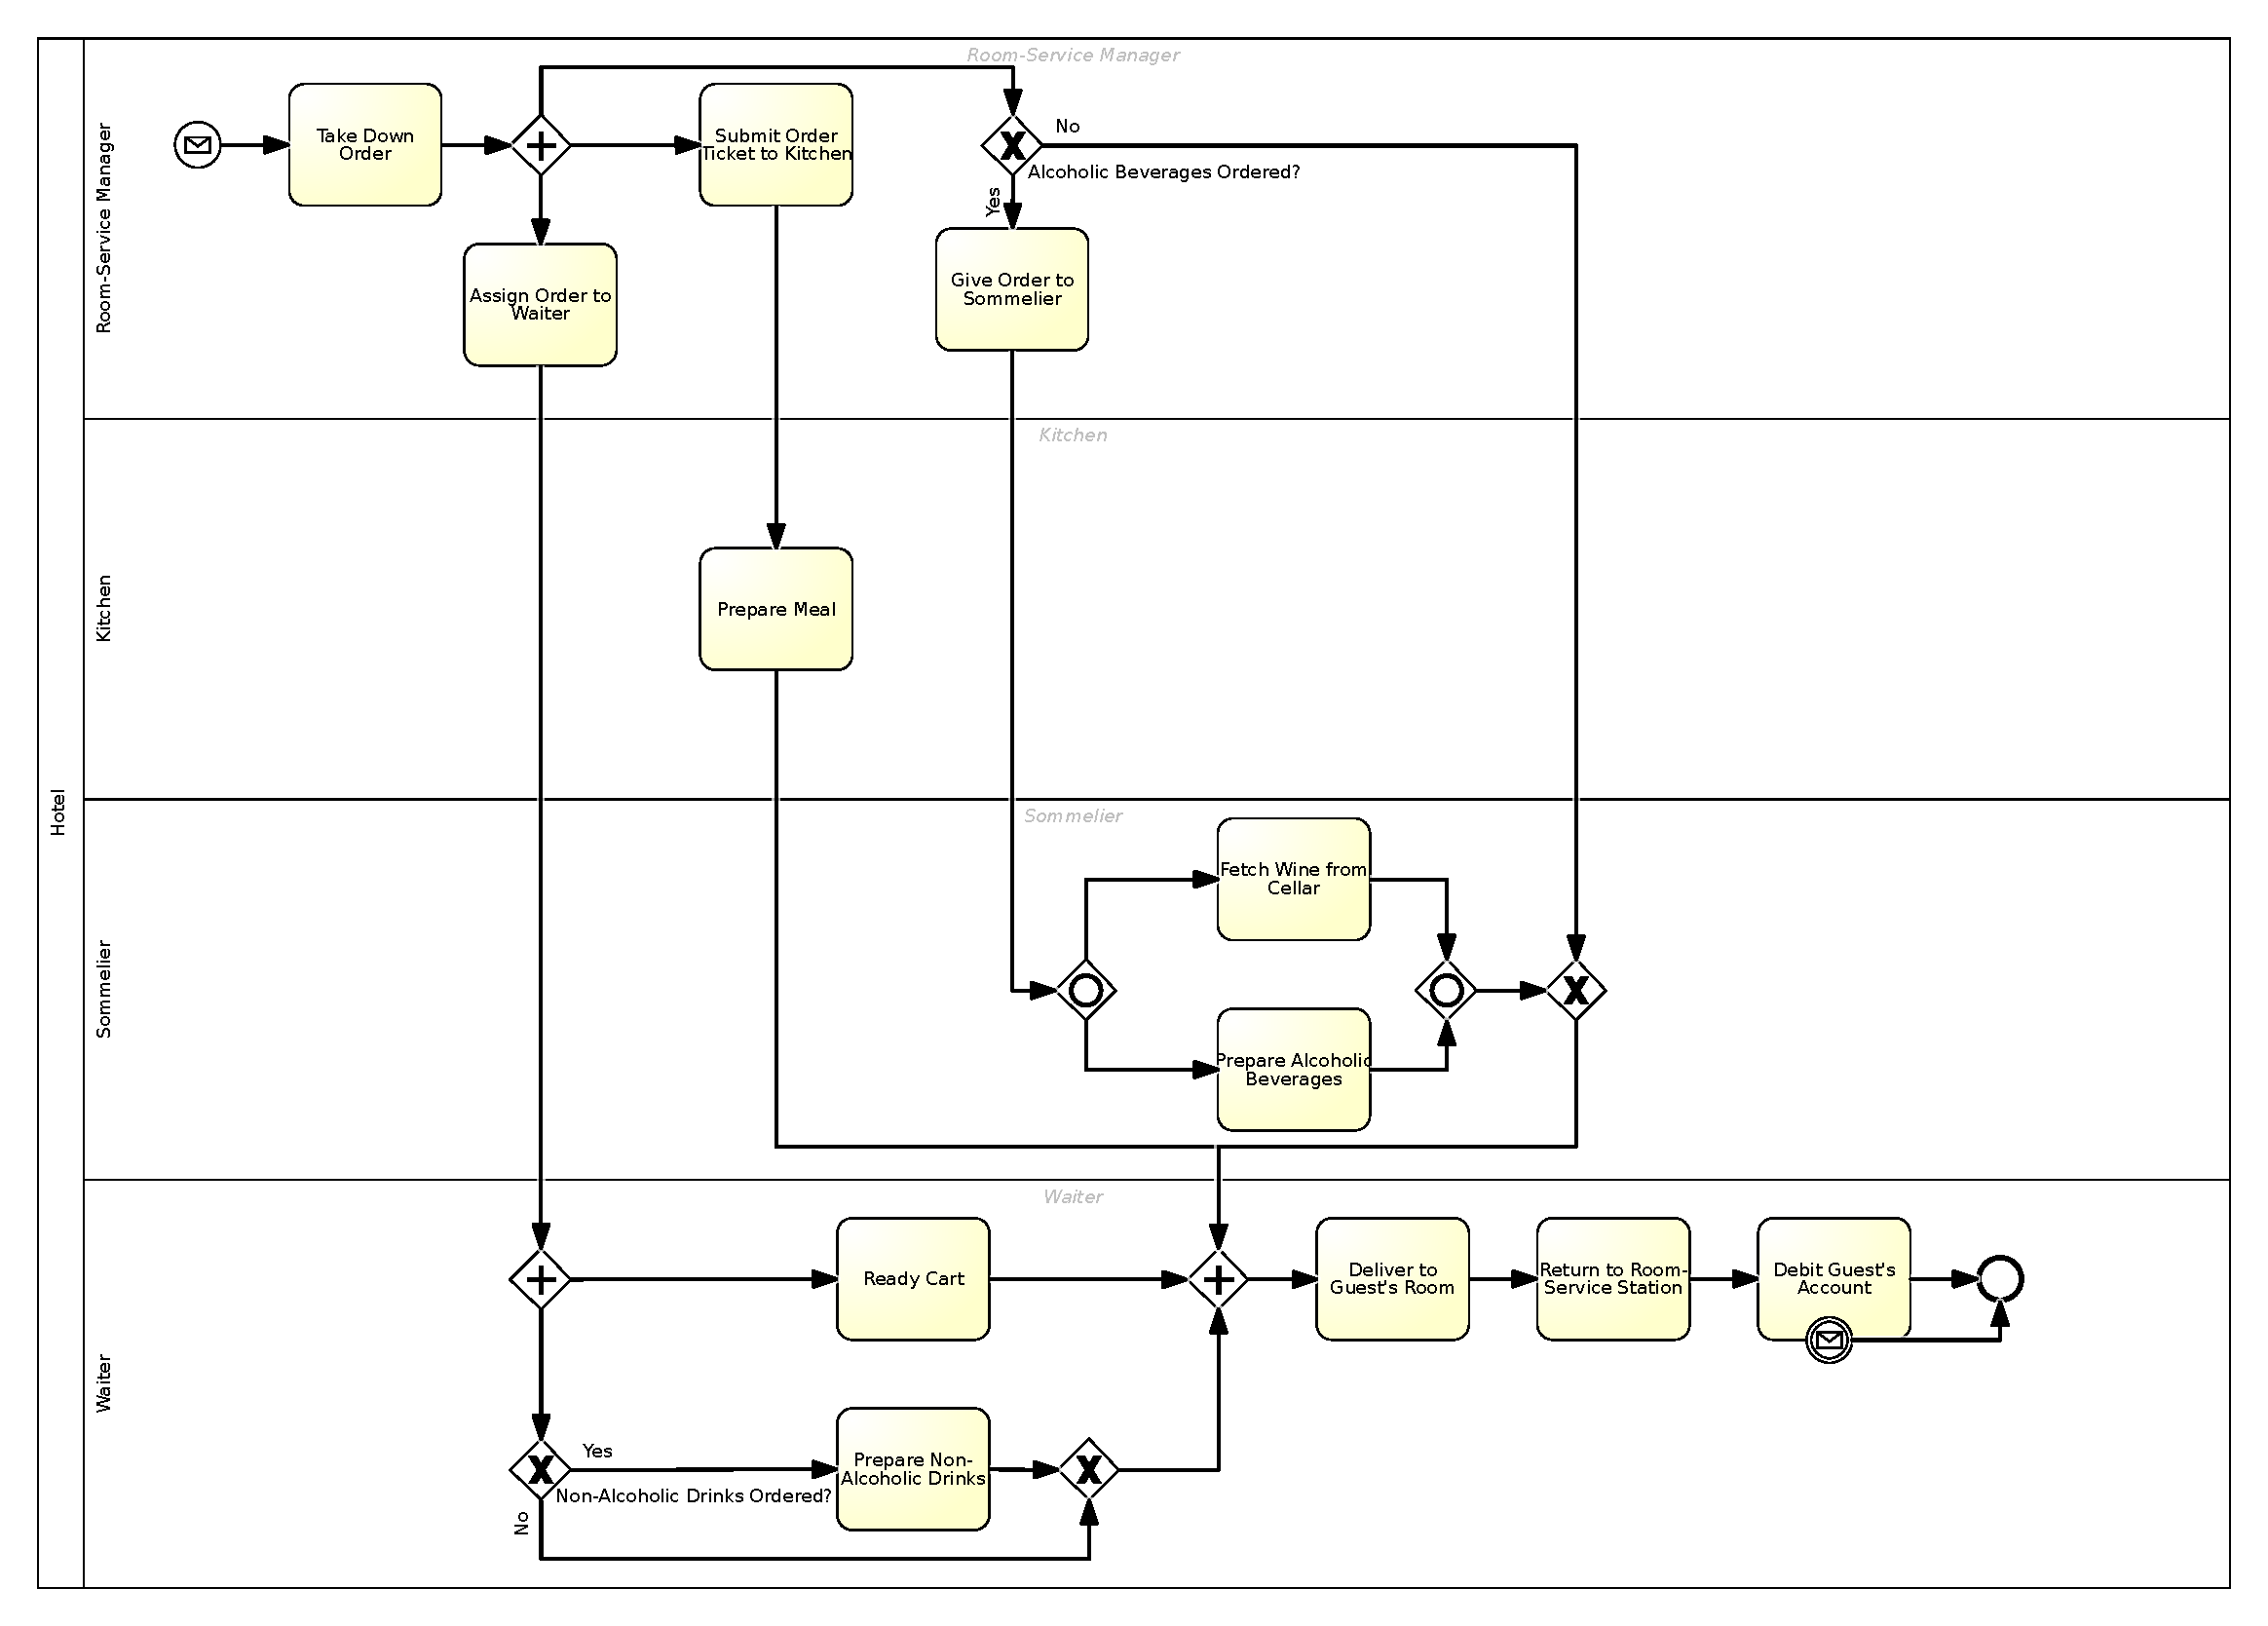
\includegraphics[width=\hsize]{./bpmn/model3.pdf}
	\caption{Hand-made BPMN diagram for process model 3}
	\label{bpmn:model3}
\end{figure}

\section{Model 4}
\begin{tcolorbox}[
	breakable,
	arc=0mm,
	left=1pt,
	right = 1pt,
	boxrule=0mm,
	colback = {white},
	]
	\texttt{\input{./models/model4.txt}}
\end{tcolorbox}
\captionof{textdesc}{Text description for model 4}
\label{txt:model4}

{\scriptsize
	\begin{longtable}{|p{0.03 \hsize}|p{0.25 \hsize}|p{0.15 \hsize}|p{0.2 \hsize}|p{0.1 \hsize}|p{0.1 \hsize}|}
		\hline
		Order & Activity & Condition & Who & Subprocess & Terminated.
		\\\hline\hline
		\csvreader[late after line=\\\hline]
		{./results/model4_intermediate_model.csv}
		{Order=\Order,Activity=\Activity,Condition=\Condition,Who=\Who,Subprocess=\Subprocess,Terminated=\Terminated}
		{\Order & \Activity & \Condition & \Who & \Subprocess & \Terminated}
		\caption{Spreadsheet-based description for process model 4}
		\label{csv:model4}
	\end{longtable}
}

\begin{figure}[H]
	\centering
	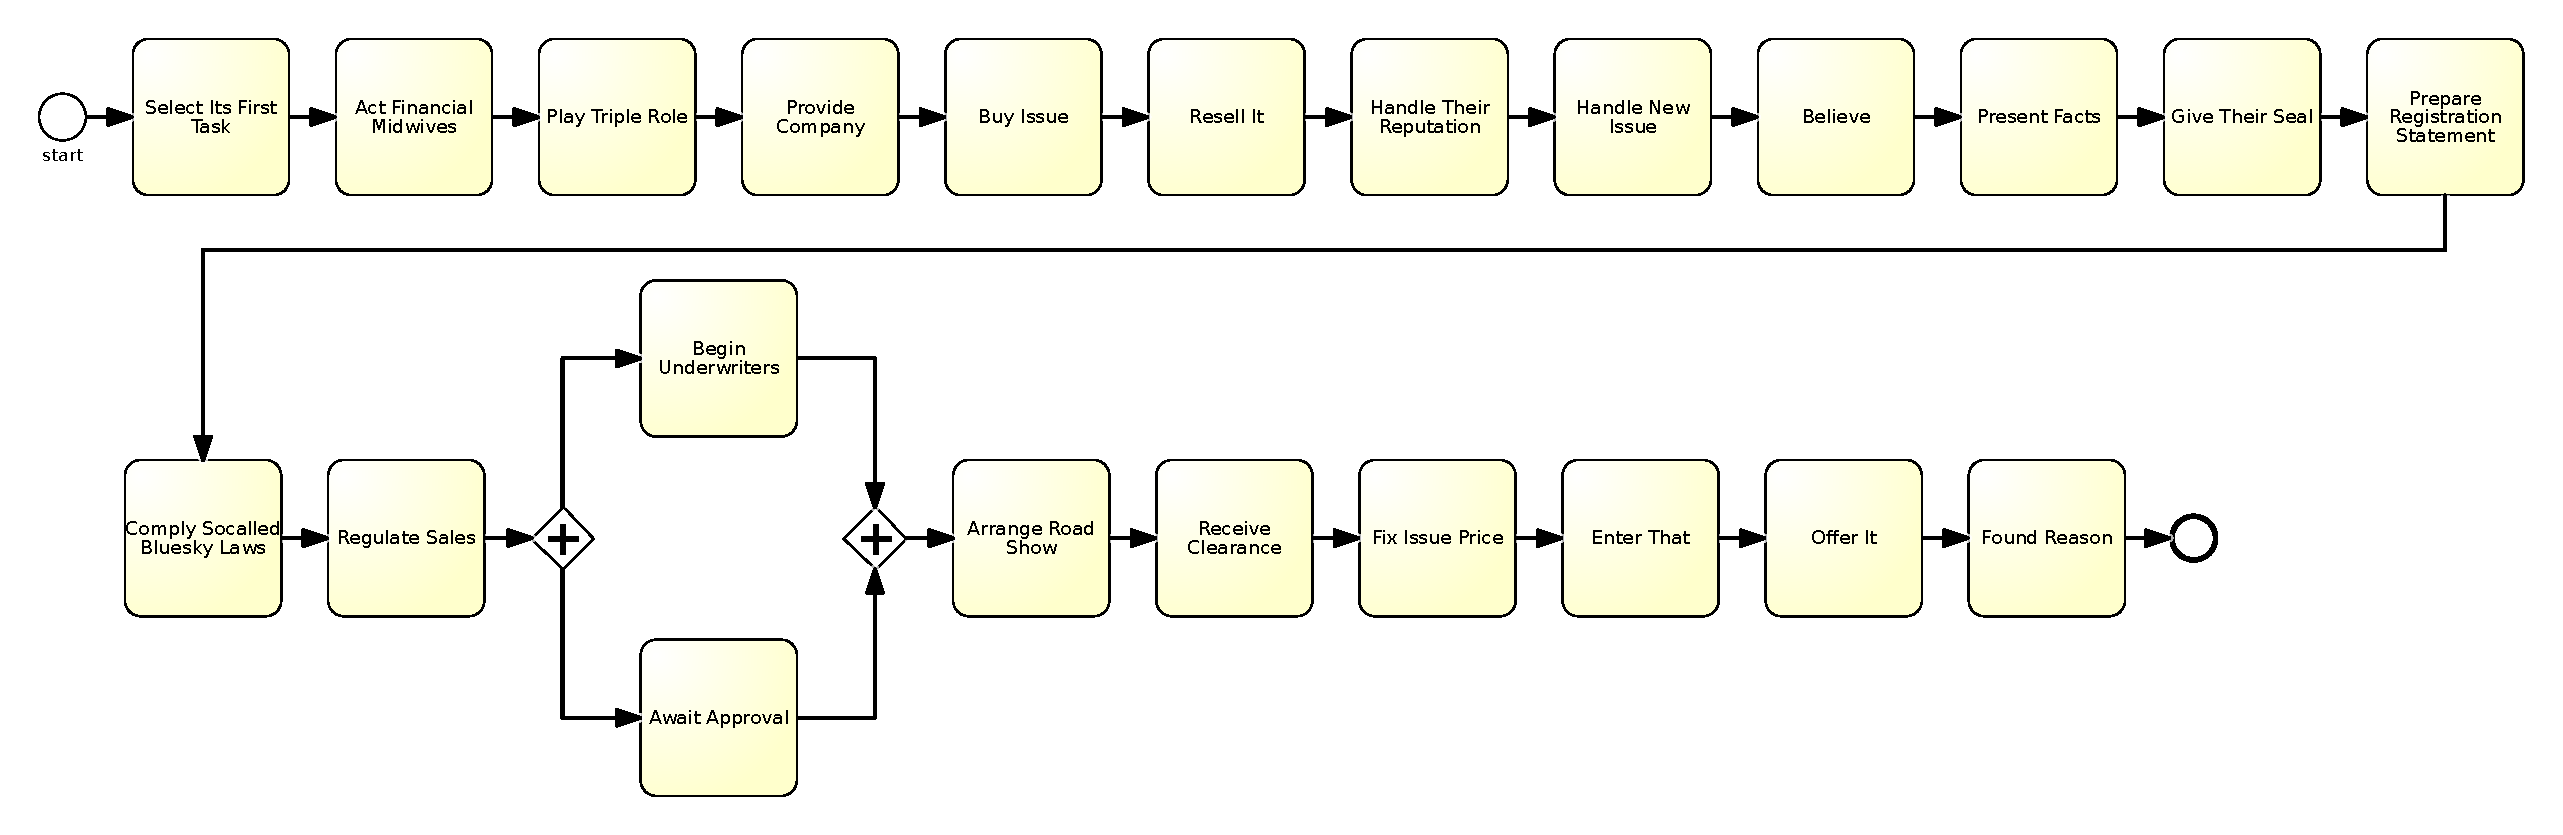
\includegraphics[scale=0.35]{./generated_bpmn/model4.pdf}
	\caption{BPMN diagram for process model 4 generated from spreadsheet-based model}
	\label{bpmn:generated_model4}
\end{figure}

\begin{figure}[H]
	\centering
	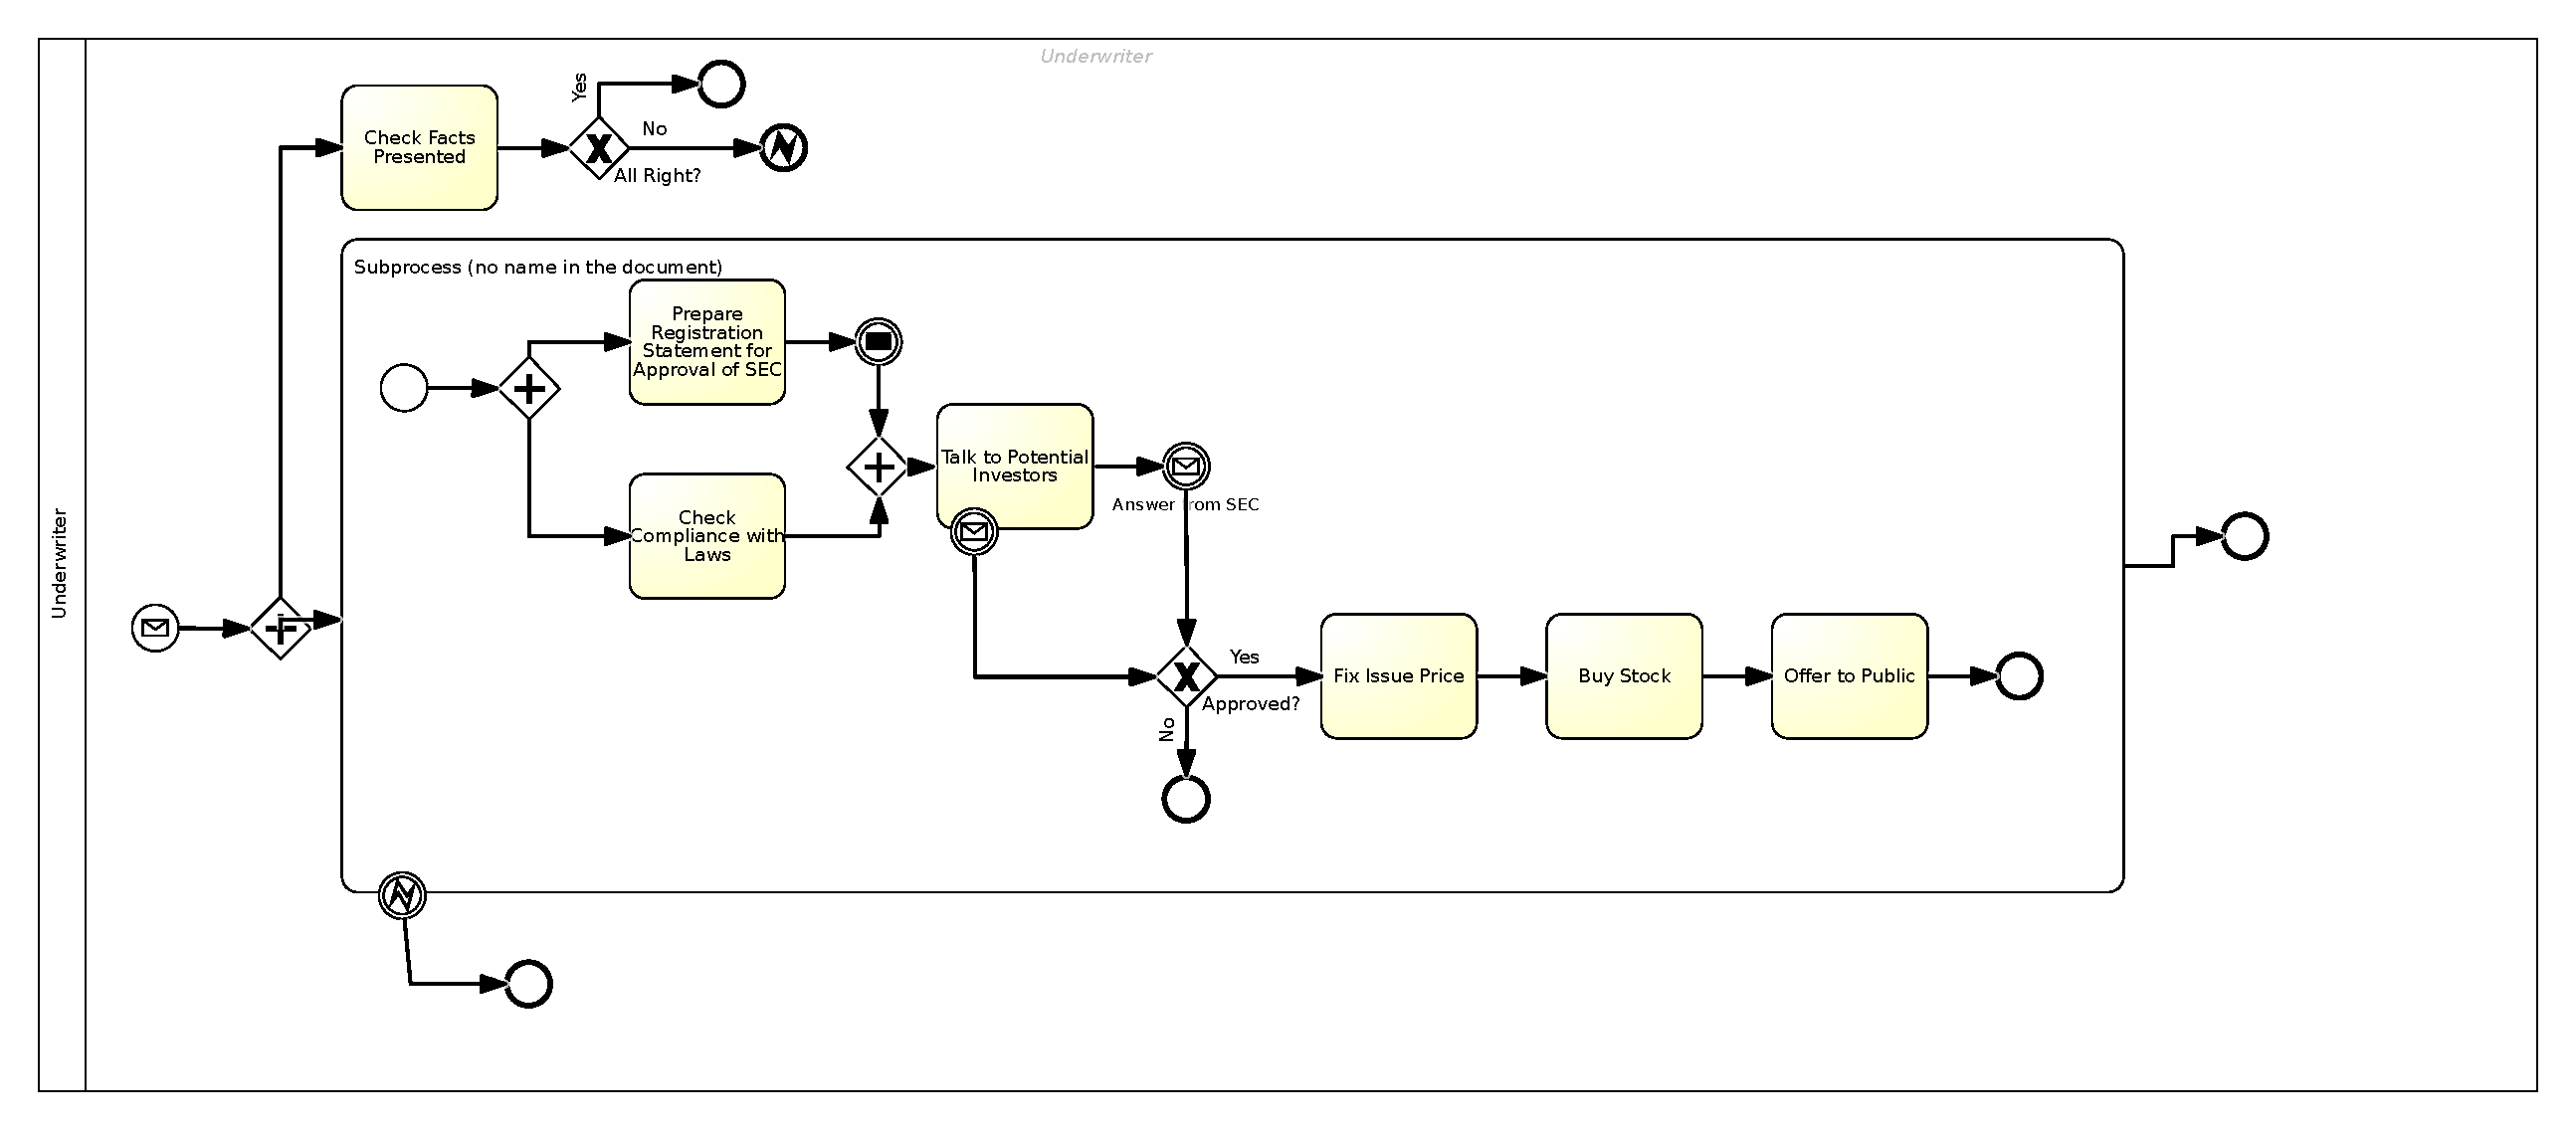
\includegraphics[width=\hsize]{./bpmn/model4.pdf}
	\caption{Hand-made BPMN diagram for process model 4}
	\label{bpmn:model4}
\end{figure}

\section{Model 5}
\begin{tcolorbox}[
	breakable,
	arc=0mm,
	left=1pt,
	right = 1pt,
	boxrule=0mm,
	colback = {white},
	]
	\texttt{\input{./models/model5.txt}}
\end{tcolorbox}
\captionof{textdesc}{Text description for model 5}
\label{txt:model5}

{\scriptsize
	\begin{longtable}{|p{0.03 \hsize}|p{0.25 \hsize}|p{0.15 \hsize}|p{0.2 \hsize}|p{0.1 \hsize}|p{0.1 \hsize}|}
		\hline
		Order & Activity & Condition & Who & Subprocess & Terminated.
		\\\hline\hline
		\csvreader[late after line=\\\hline]
		{./results/model5_intermediate_model.csv}
		{Order=\Order,Activity=\Activity,Condition=\Condition,Who=\Who,Subprocess=\Subprocess,Terminated=\Terminated}
		{\Order & \Activity & \Condition & \Who & \Subprocess & \Terminated}
		\caption{Spreadsheet-based description for process model 5}
		\label{csv:model5}
	\end{longtable}
}

\begin{figure}[H]
	\centering
	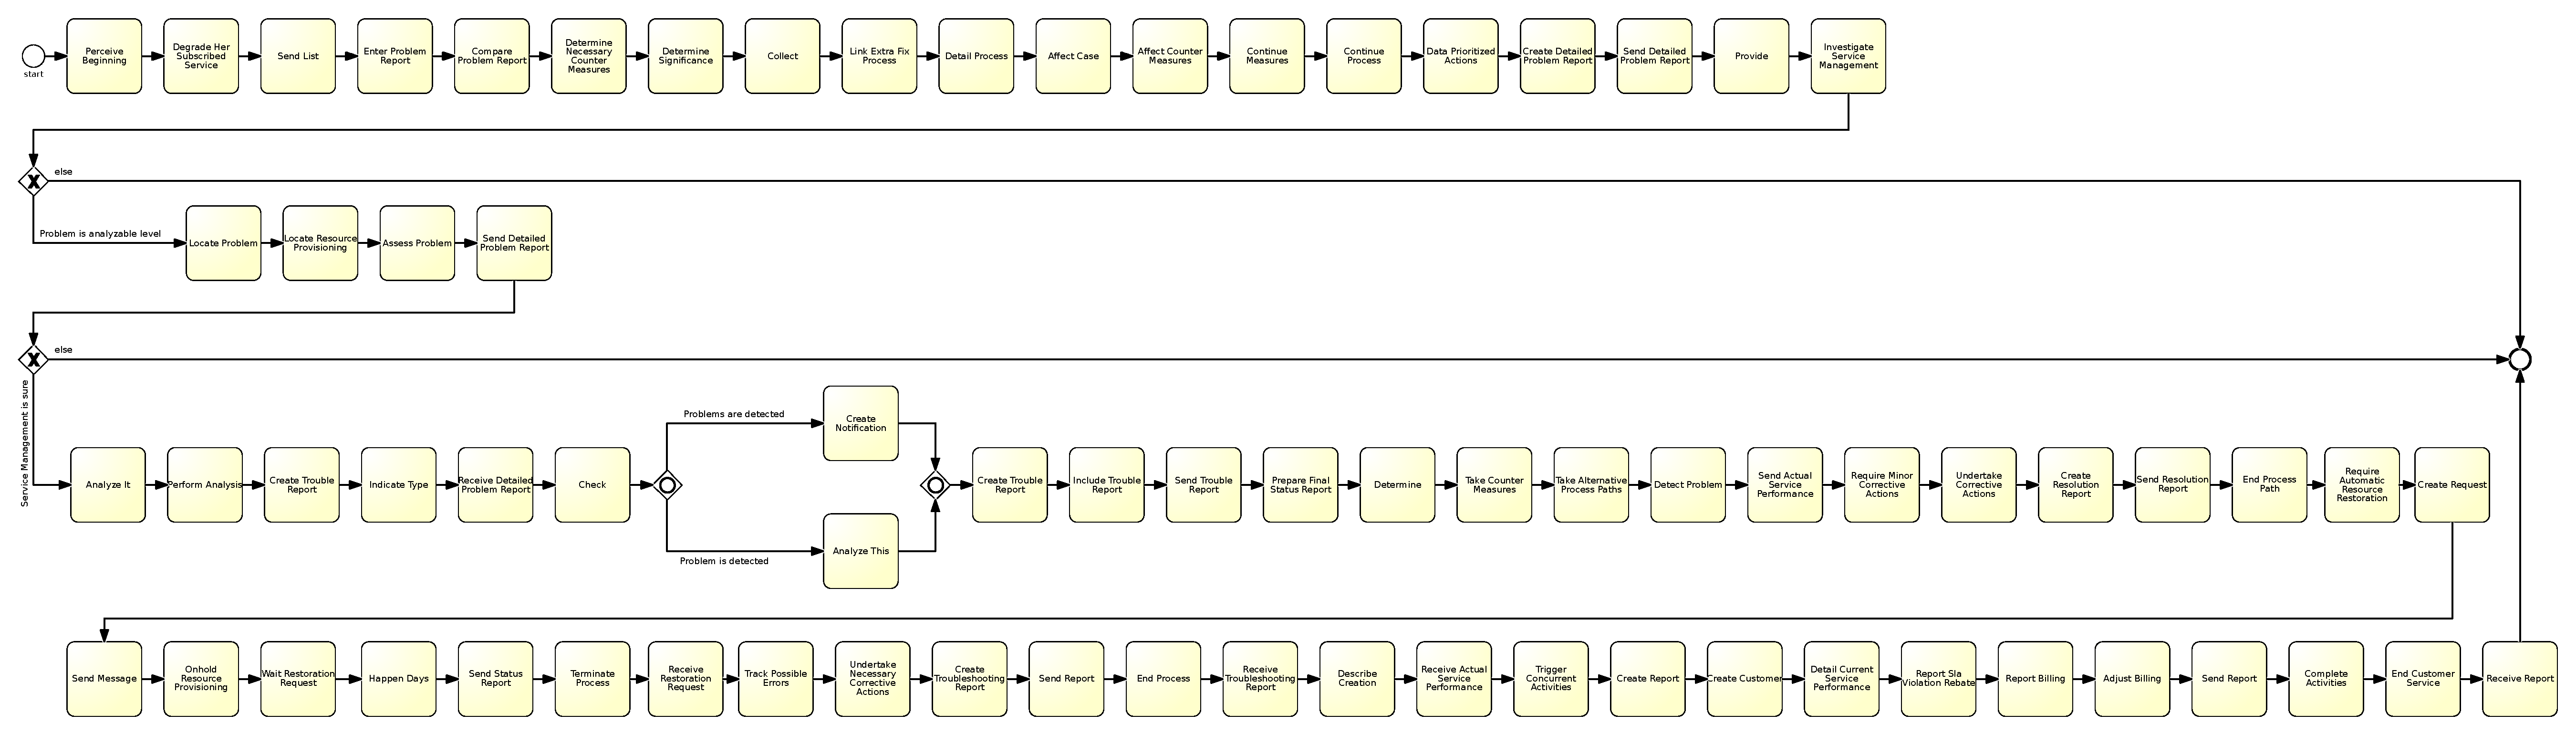
\includegraphics[width=0.95\textheight, angle=90]{./generated_bpmn/model5.pdf}
	\caption{BPMN diagram for process model 5 generated from spreadsheet-based model}
	\label{bpmn:generated_model5}
\end{figure}

\begin{figure}[H]
	\centering
	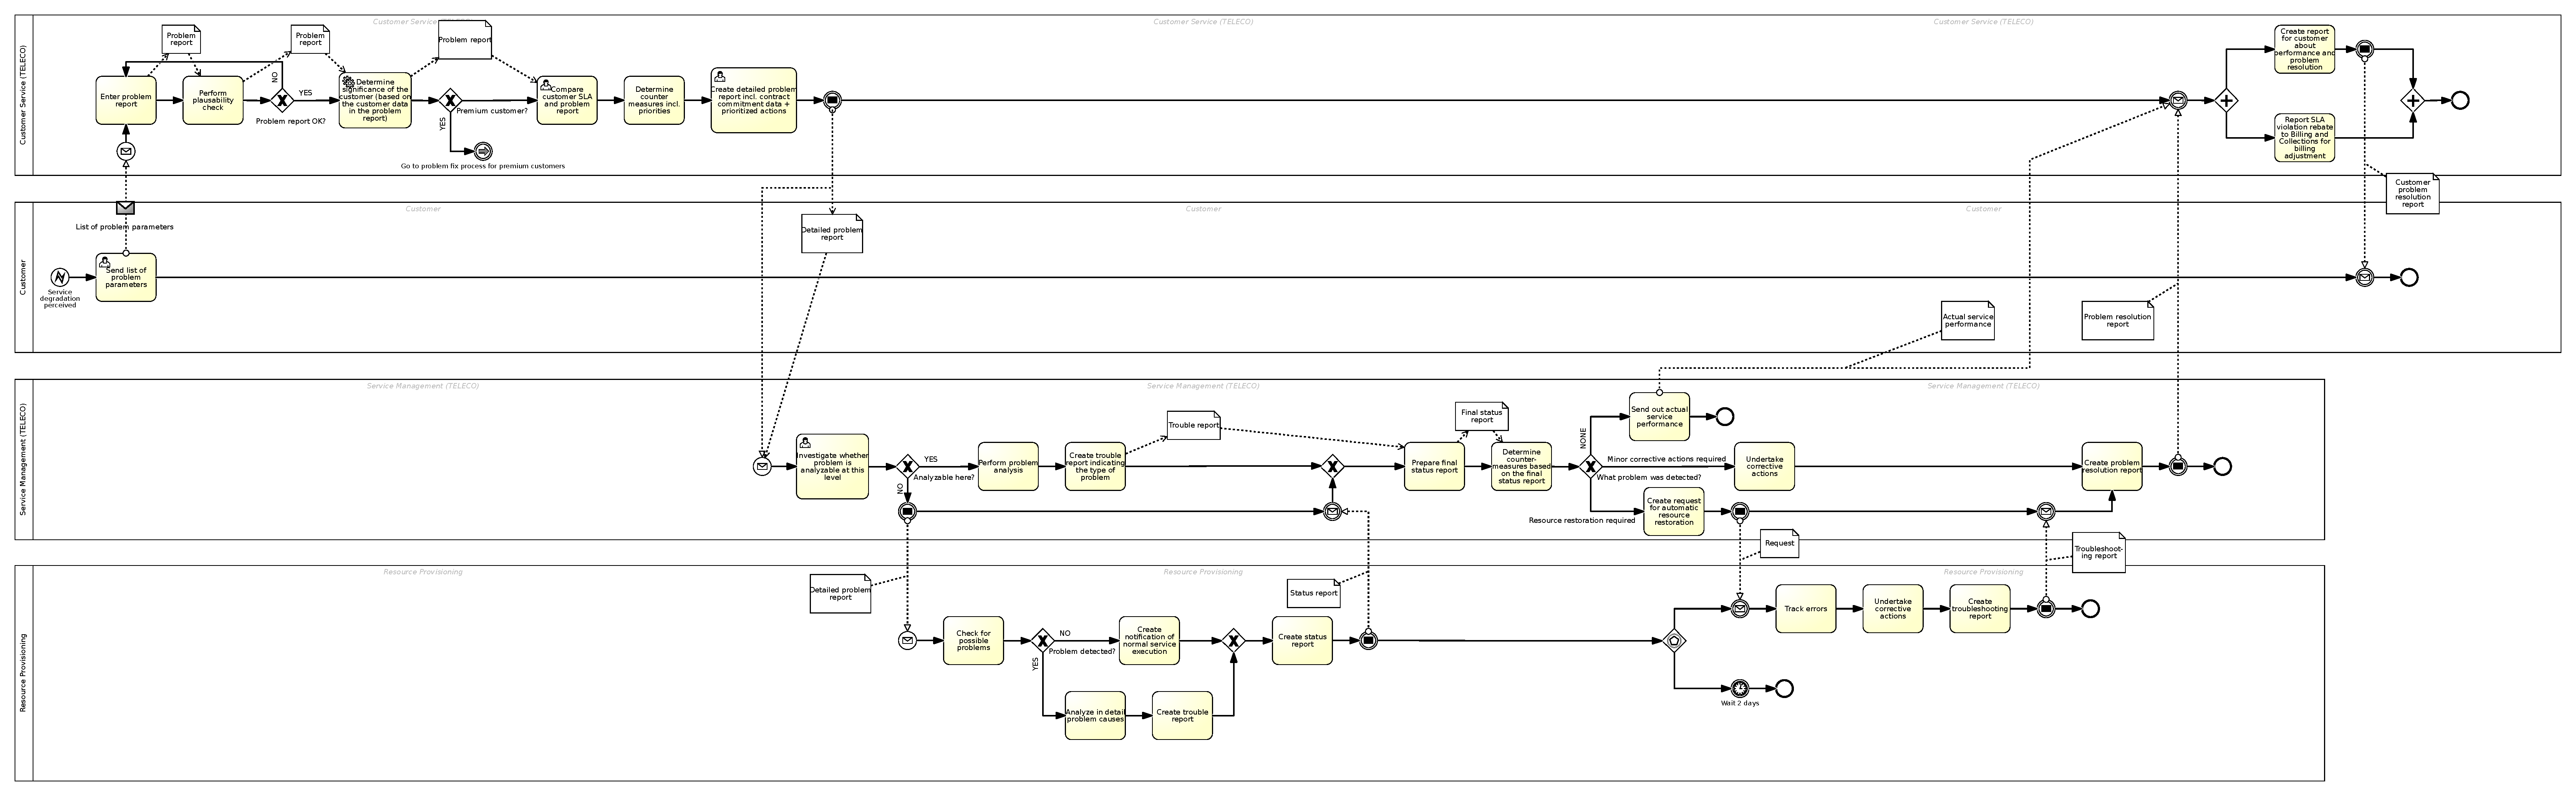
\includegraphics[width=0.95\textheight, angle=90]{./bpmn/model5.pdf}
	\caption{Hand-made BPMN diagram for process model 5}
	\label{bpmn:model5}
\end{figure}

\section{Model 6}
\begin{tcolorbox}[
	breakable,
	arc=0mm,
	left=1pt,
	right = 1pt,
	boxrule=0mm,
	colback = {white},
	]
	\texttt{\input{./models/model6.txt}}
\end{tcolorbox}
\captionof{textdesc}{Text description for model 6}
\label{txt:model6}
\newpage

{\scriptsize
	\begin{longtable}{|p{0.03 \hsize}|p{0.25 \hsize}|p{0.15 \hsize}|p{0.2 \hsize}|p{0.1 \hsize}|p{0.1 \hsize}|}
		\hline
		Order & Activity & Condition & Who & Subprocess & Terminated.
		\\\hline\hline
		\csvreader[late after line=\\\hline]
		{./results/model6_intermediate_model.csv}
		{Order=\Order,Activity=\Activity,Condition=\Condition,Who=\Who,Subprocess=\Subprocess,Terminated=\Terminated}
		{\Order & \Activity & \Condition & \Who & \Subprocess & \Terminated}
		\caption{Spreadsheet-based description for process model 6}
		\label{csv:model6}
	\end{longtable}
}

\begin{figure}[H]
	\centering
	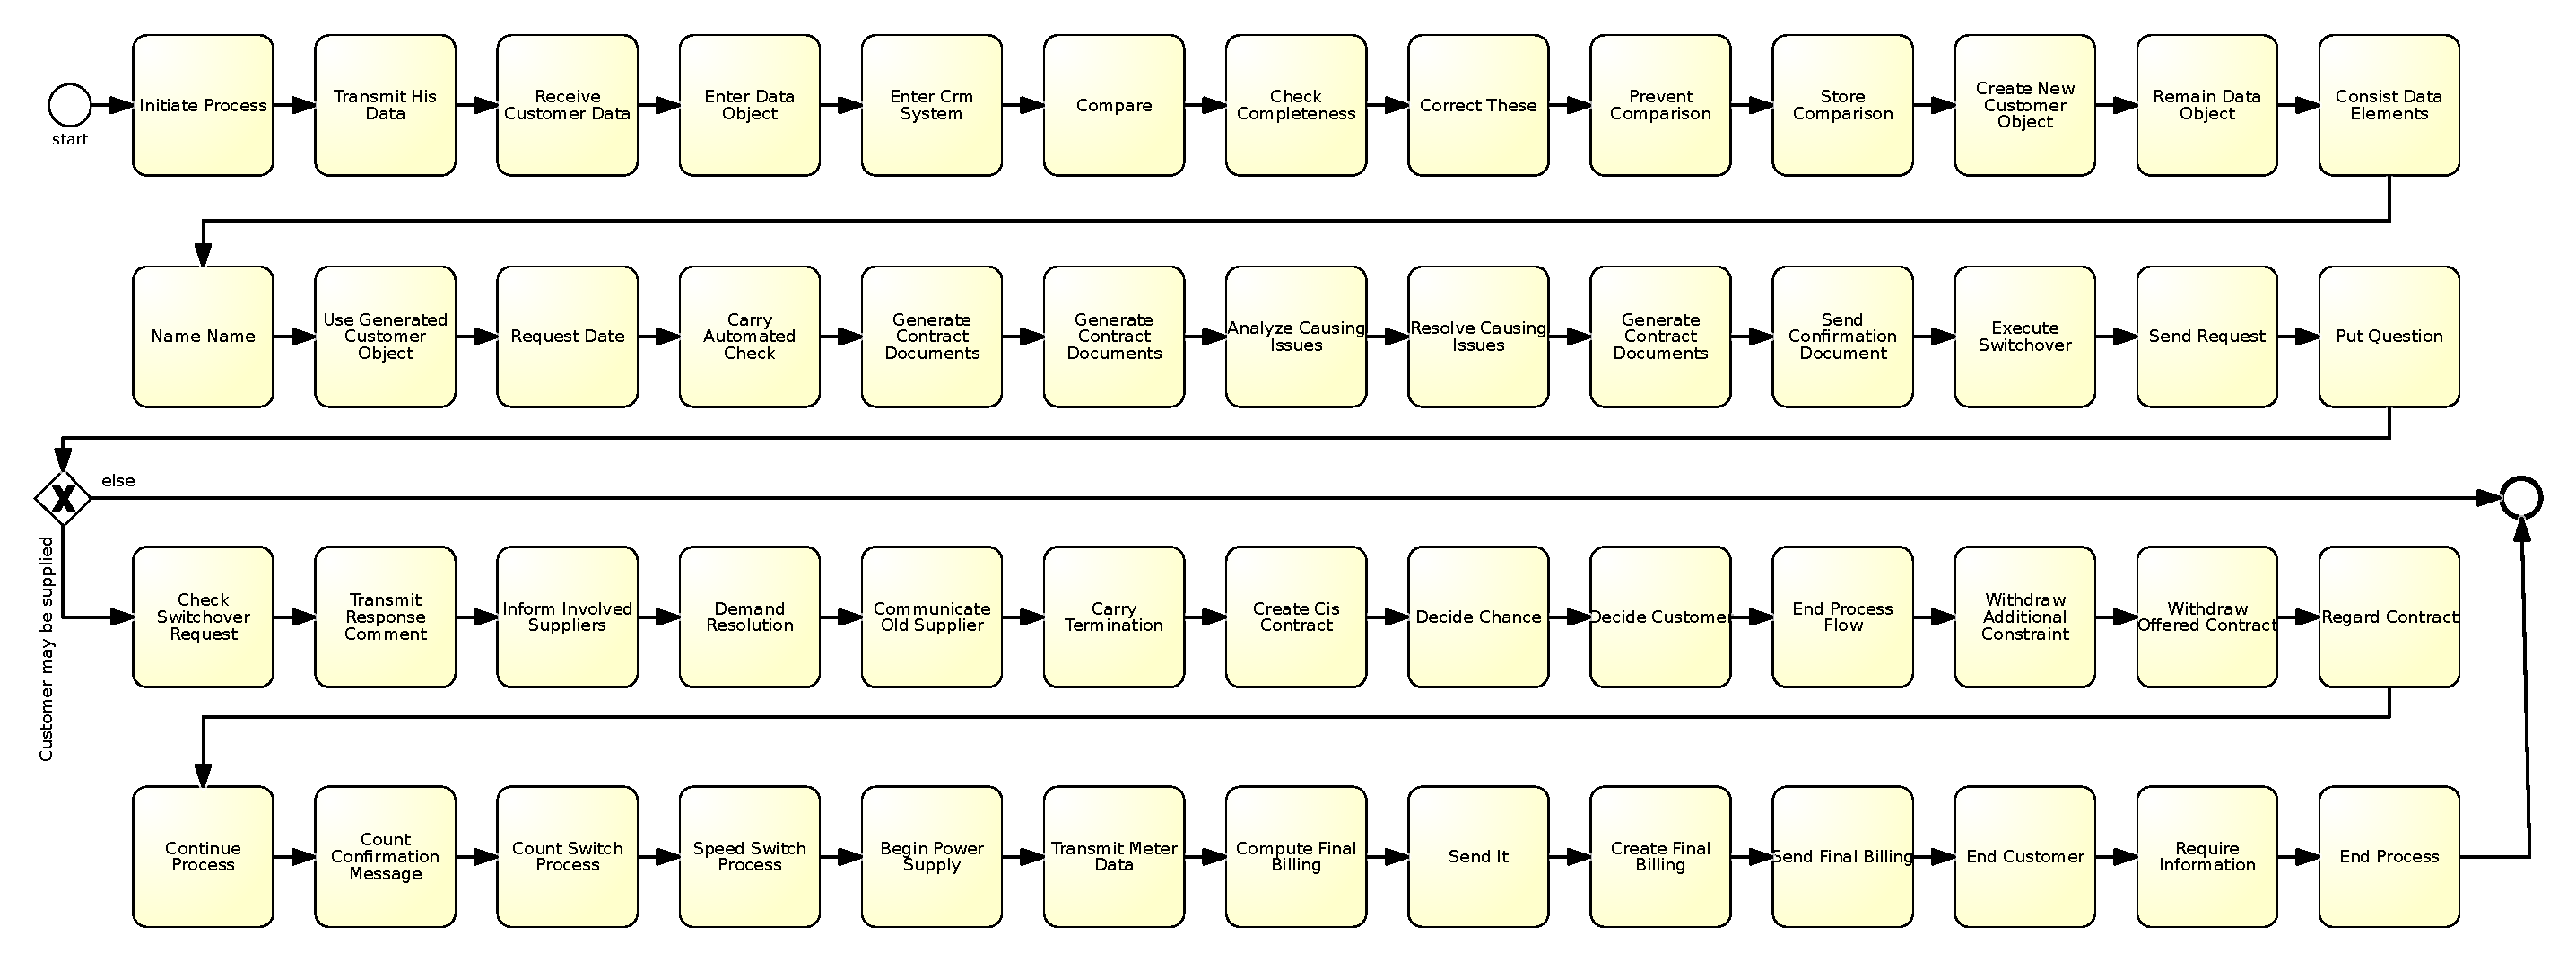
\includegraphics[width=0.95\textheight, angle=90]{./generated_bpmn/model6.pdf}
	\caption{BPMN diagram for process model 6 generated from spreadsheet-based model}
	\label{bpmn:generated_model6}
\end{figure}

\begin{figure}[H]
	\centering
	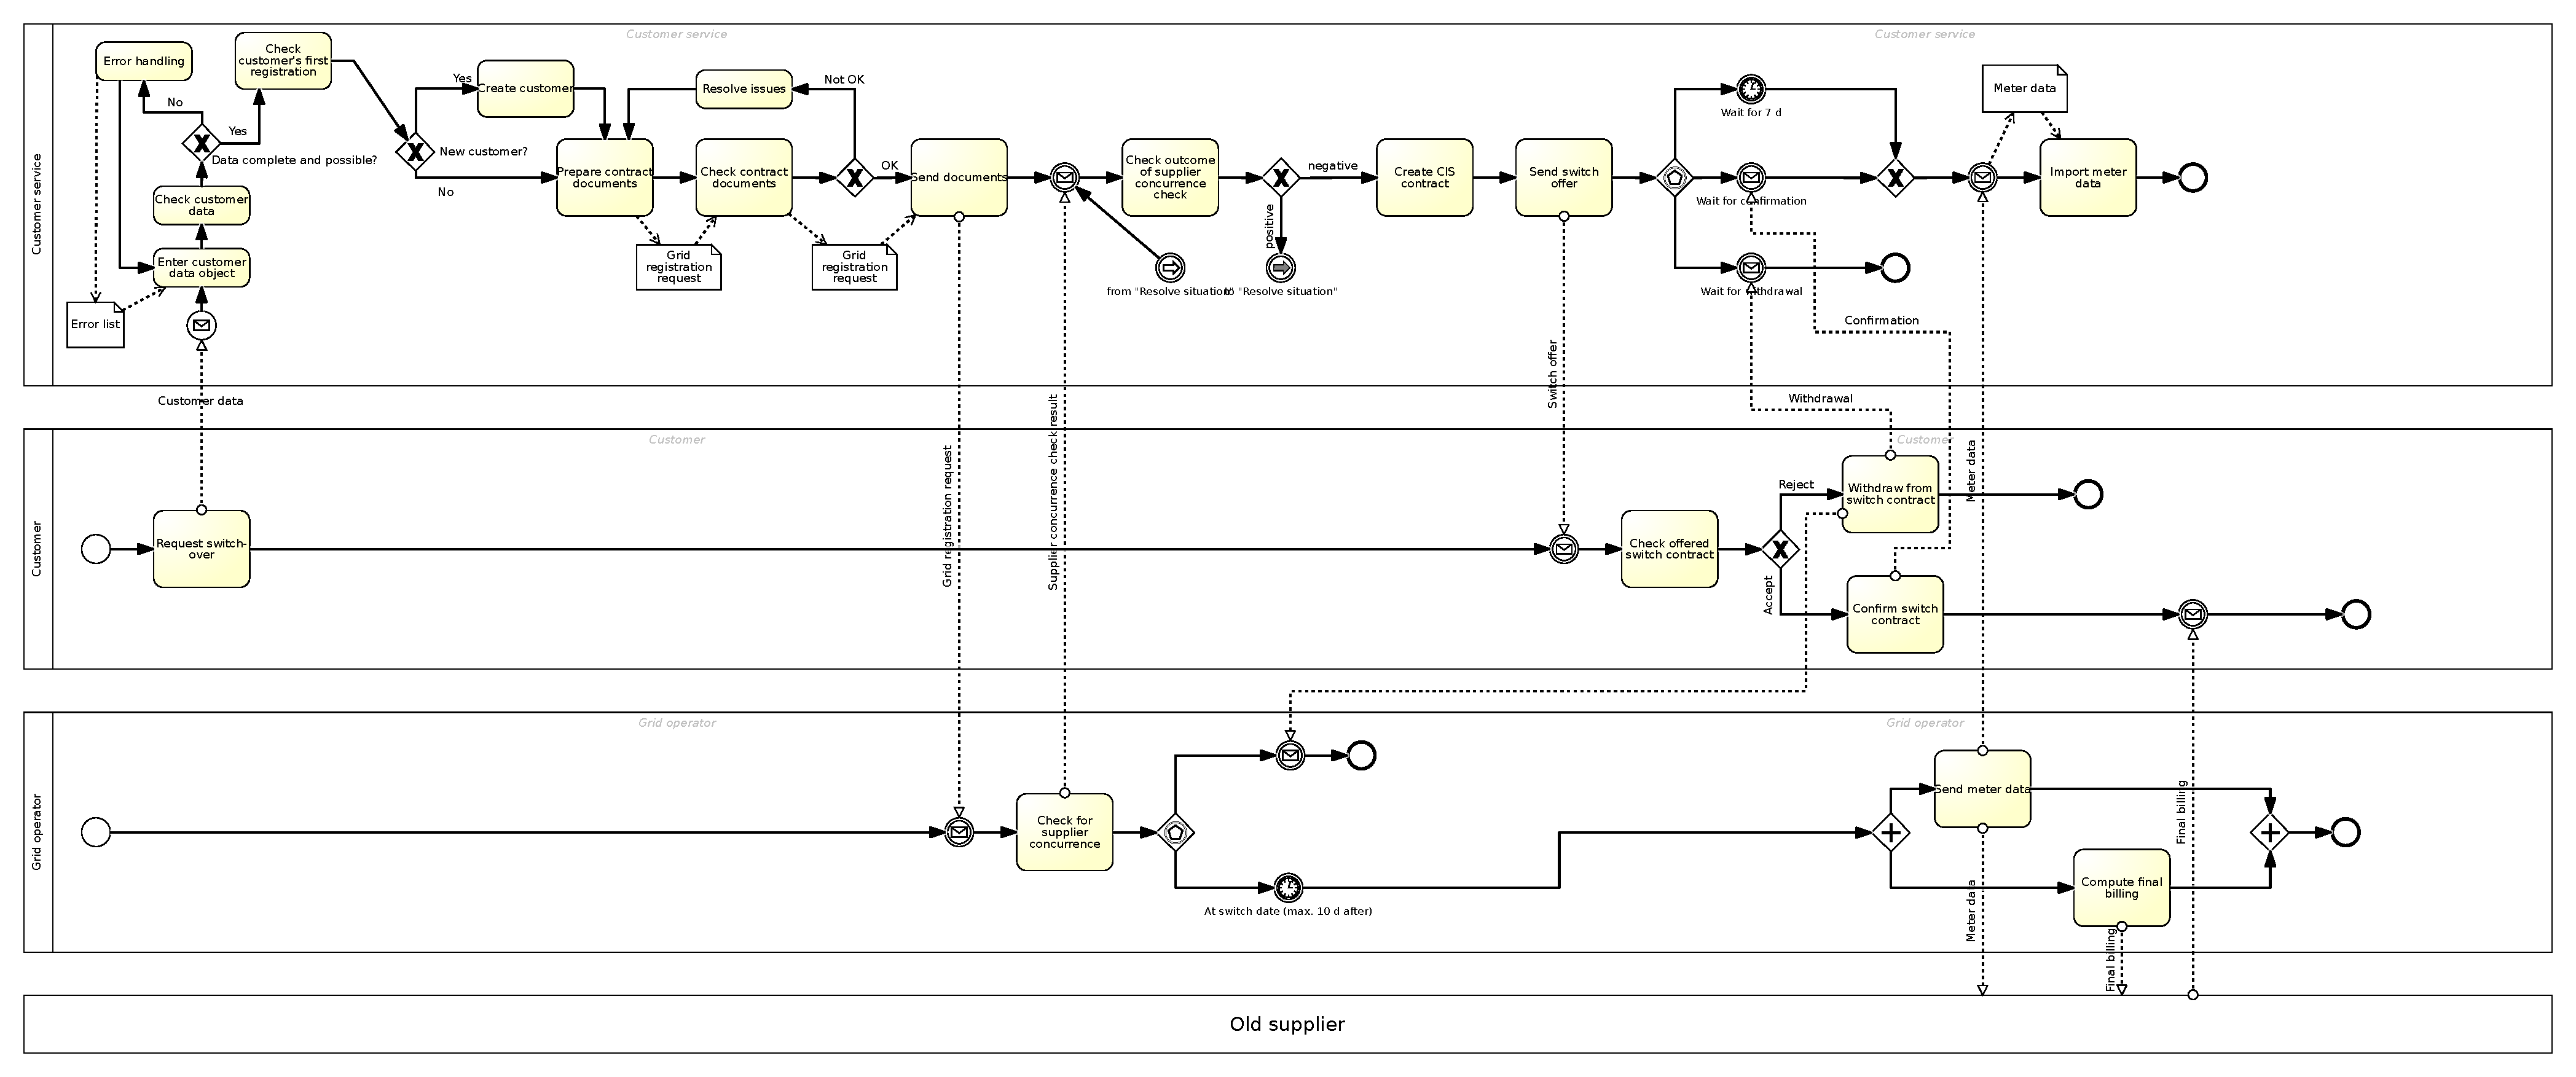
\includegraphics[width=0.95\textheight, angle=90]{./bpmn/model6.pdf}
	\caption{Hand-made BPMN diagram for process model 6}
	\label{bpmn:model6}
\end{figure}

\section{Model 7}
\begin{tcolorbox}[
	breakable,
	arc=0mm,
	left=1pt,
	right = 1pt,
	boxrule=0mm,
	colback = {white},
	]
	\texttt{\input{./models/model7.txt}}
\end{tcolorbox}
\captionof{textdesc}{Text description for model 7}
\label{txt:model7}

{\scriptsize
	\begin{longtable}{|p{0.03 \hsize}|p{0.25 \hsize}|p{0.15 \hsize}|p{0.2 \hsize}|p{0.1 \hsize}|p{0.1 \hsize}|}
		\hline
		Order & Activity & Condition & Who & Subprocess & Terminated.
		\\\hline\hline
		\csvreader[late after line=\\\hline]
		{./results/model7_intermediate_model.csv}
		{Order=\Order,Activity=\Activity,Condition=\Condition,Who=\Who,Subprocess=\Subprocess,Terminated=\Terminated}
		{\Order & \Activity & \Condition & \Who & \Subprocess & \Terminated}
		\caption{Spreadsheet-based description for process model 7}
		\label{csv:model7}
	\end{longtable}
}

\begin{figure}[H]
	\centering
	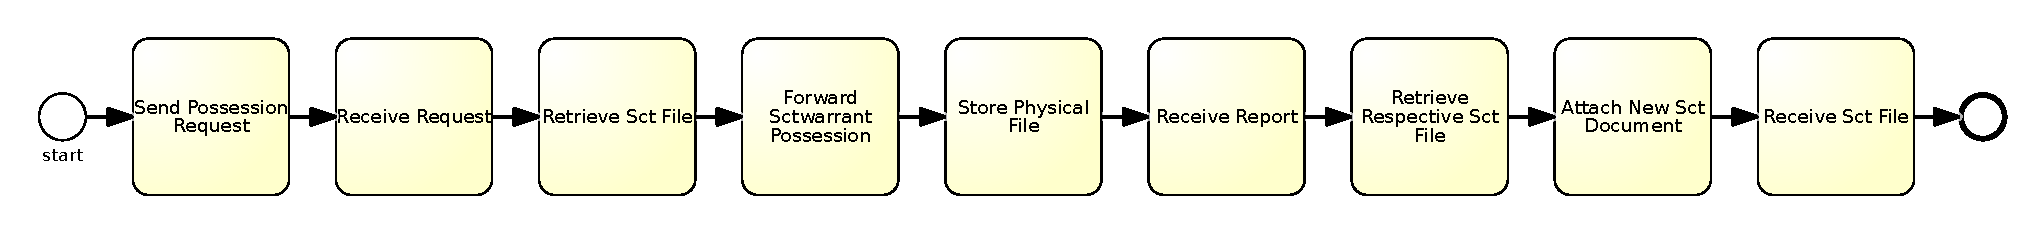
\includegraphics[width=\hsize]{./generated_bpmn/model7.pdf}
	\caption{BPMN diagram for process model 7 generated from spreadsheet-based model}
	\label{bpmn:generated_model7}
\end{figure}

\begin{figure}[H]
	\centering
	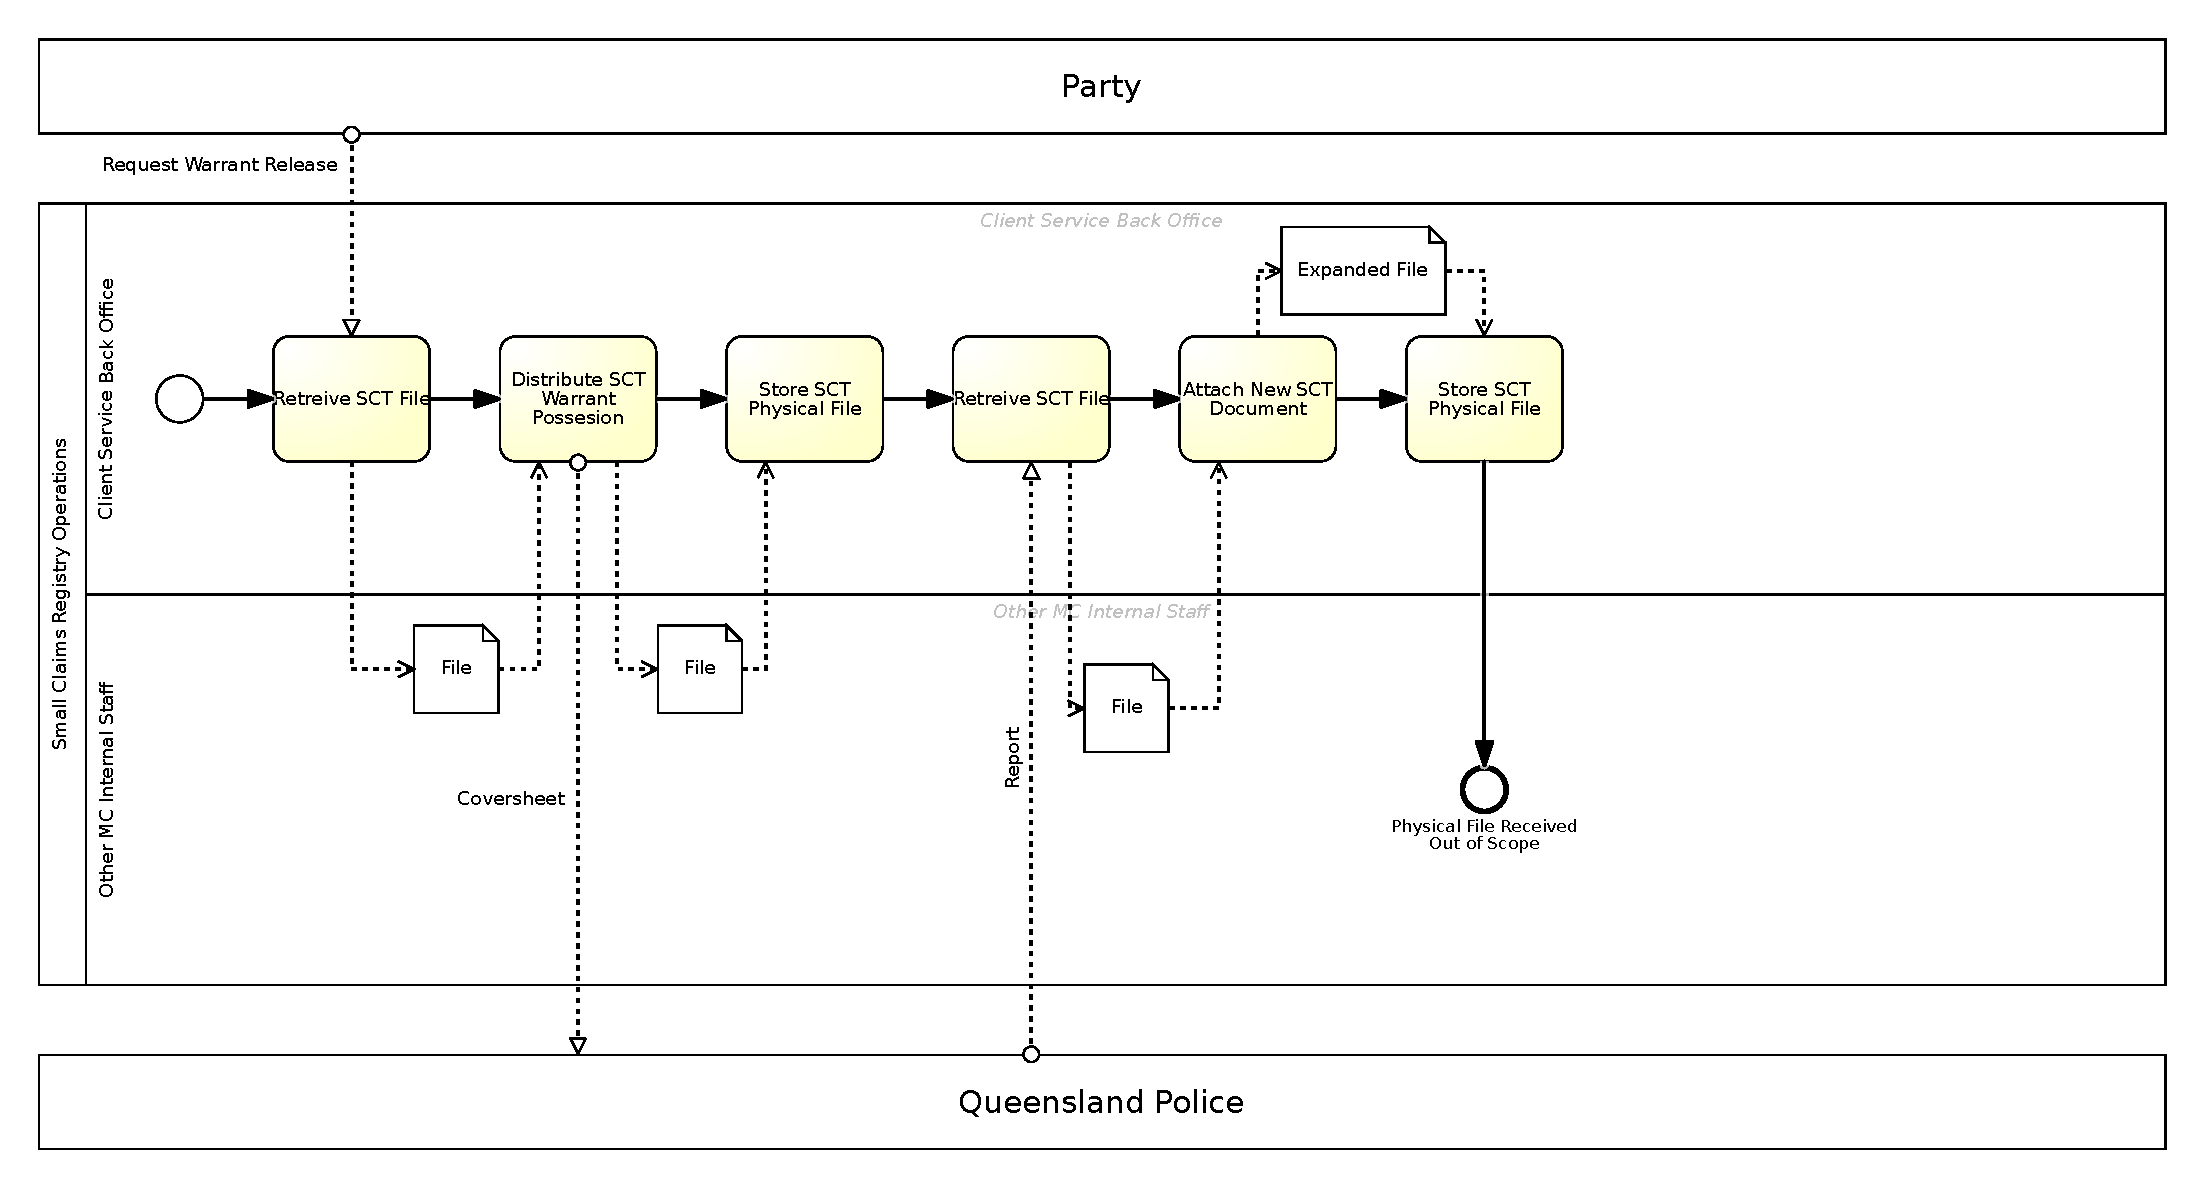
\includegraphics[width=\hsize]{./bpmn/model7.pdf}
	\caption{Hand-made BPMN diagram for process model 7}
	\label{bpmn:model7}
\end{figure}

\section{Model 8}
\begin{tcolorbox}[
	breakable,
	arc=0mm,
	left=1pt,
	right = 1pt,
	boxrule=0mm,
	colback = {white},
	]
	\texttt{\input{./models/model8.txt}}
\end{tcolorbox}
\captionof{textdesc}{Text description for model 8}
\label{txt:model8}
\newpage
{\scriptsize
	\begin{longtable}{|p{0.03 \hsize}|p{0.25 \hsize}|p{0.15 \hsize}|p{0.2 \hsize}|p{0.1 \hsize}|p{0.1 \hsize}|}
		\hline
		Order & Activity & Condition & Who & Subprocess & Terminated.
		\\\hline\hline
		\csvreader[late after line=\\\hline]
		{./results/model8_intermediate_model.csv}
		{Order=\Order,Activity=\Activity,Condition=\Condition,Who=\Who,Subprocess=\Subprocess,Terminated=\Terminated}
		{\Order & \Activity & \Condition & \Who & \Subprocess & \Terminated}
		\caption{Spreadsheet-based description for process model 8}
		\label{csv:model8}
	\end{longtable}
}

\begin{figure}[H]
	\centering
	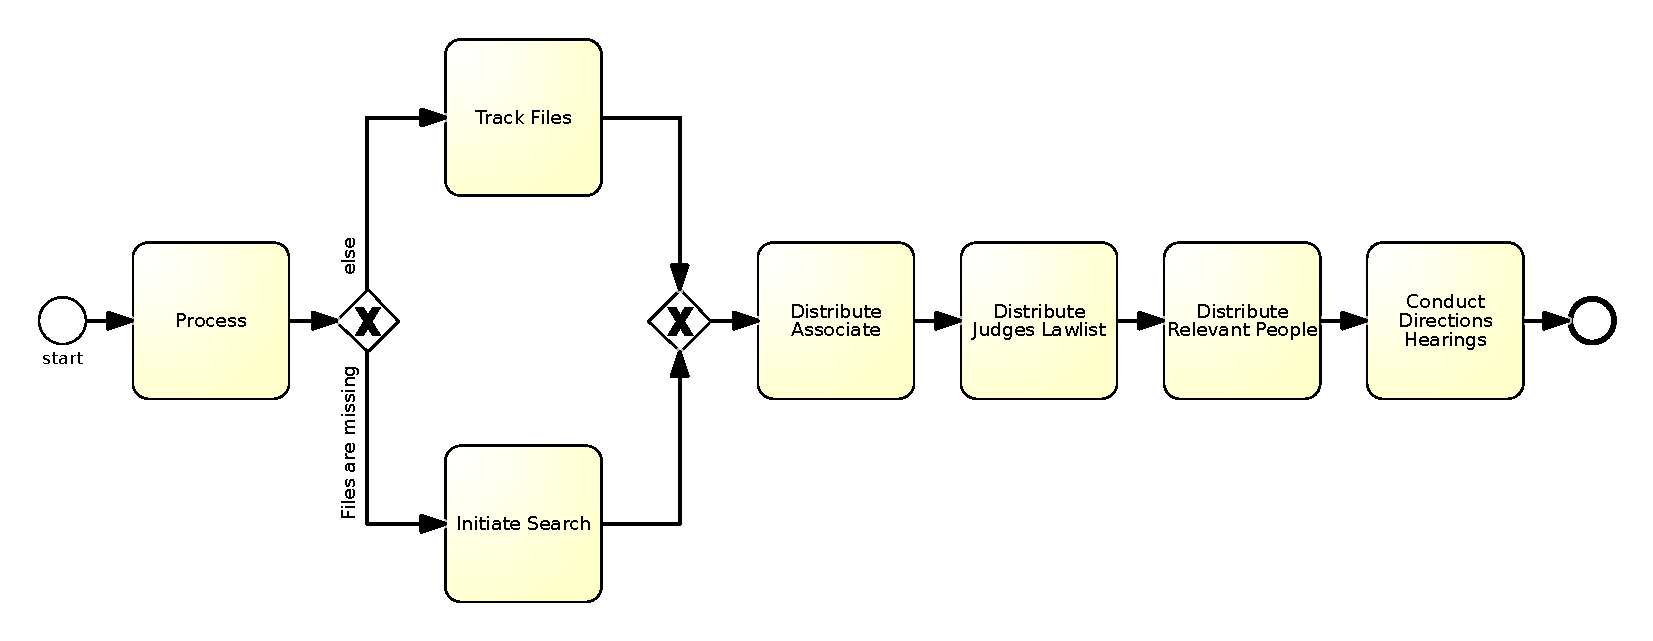
\includegraphics[width=\hsize]{./generated_bpmn/model8.pdf}
	\caption{BPMN diagram for process model 8 generated from spreadsheet-based model}
	\label{bpmn:generated_model8}
\end{figure}

\begin{figure}[H]
	\centering
	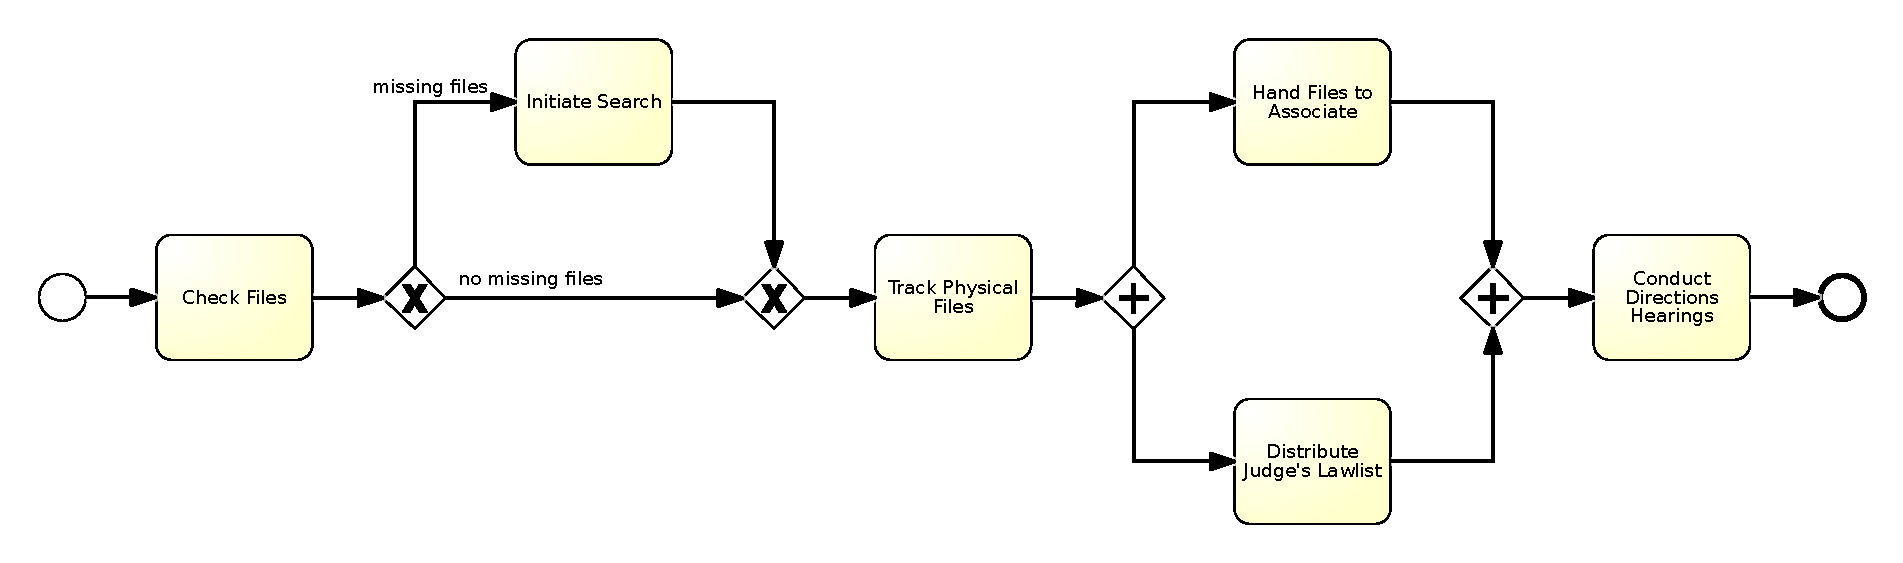
\includegraphics[width=\hsize]{./bpmn/model8.pdf}
	\caption{Hand-made BPMN diagram for process model 8}
	\label{bpmn:model8}
\end{figure}

\section{Model 9}
\begin{tcolorbox}[
	breakable,
	arc=0mm,
	left=1pt,
	right = 1pt,
	boxrule=0mm,
	colback = {white},
	]
	\texttt{\input{./models/model9.txt}}
\end{tcolorbox}
\captionof{textdesc}{Text description for model 9}
\label{txt:model9}

{\scriptsize
	\begin{longtable}{|p{0.03 \hsize}|p{0.25 \hsize}|p{0.15 \hsize}|p{0.2 \hsize}|p{0.1 \hsize}|p{0.1 \hsize}|}
		\hline
		Order & Activity & Condition & Who & Subprocess & Terminated.
		\\\hline\hline
		\csvreader[late after line=\\\hline]
		{./results/model9_intermediate_model.csv}
		{Order=\Order,Activity=\Activity,Condition=\Condition,Who=\Who,Subprocess=\Subprocess,Terminated=\Terminated}
		{\Order & \Activity & \Condition & \Who & \Subprocess & \Terminated}
		\caption{Spreadsheet-based description for process model 9}
		\label{csv:model9}
	\end{longtable}
}

\begin{figure}[H]
	\centering
	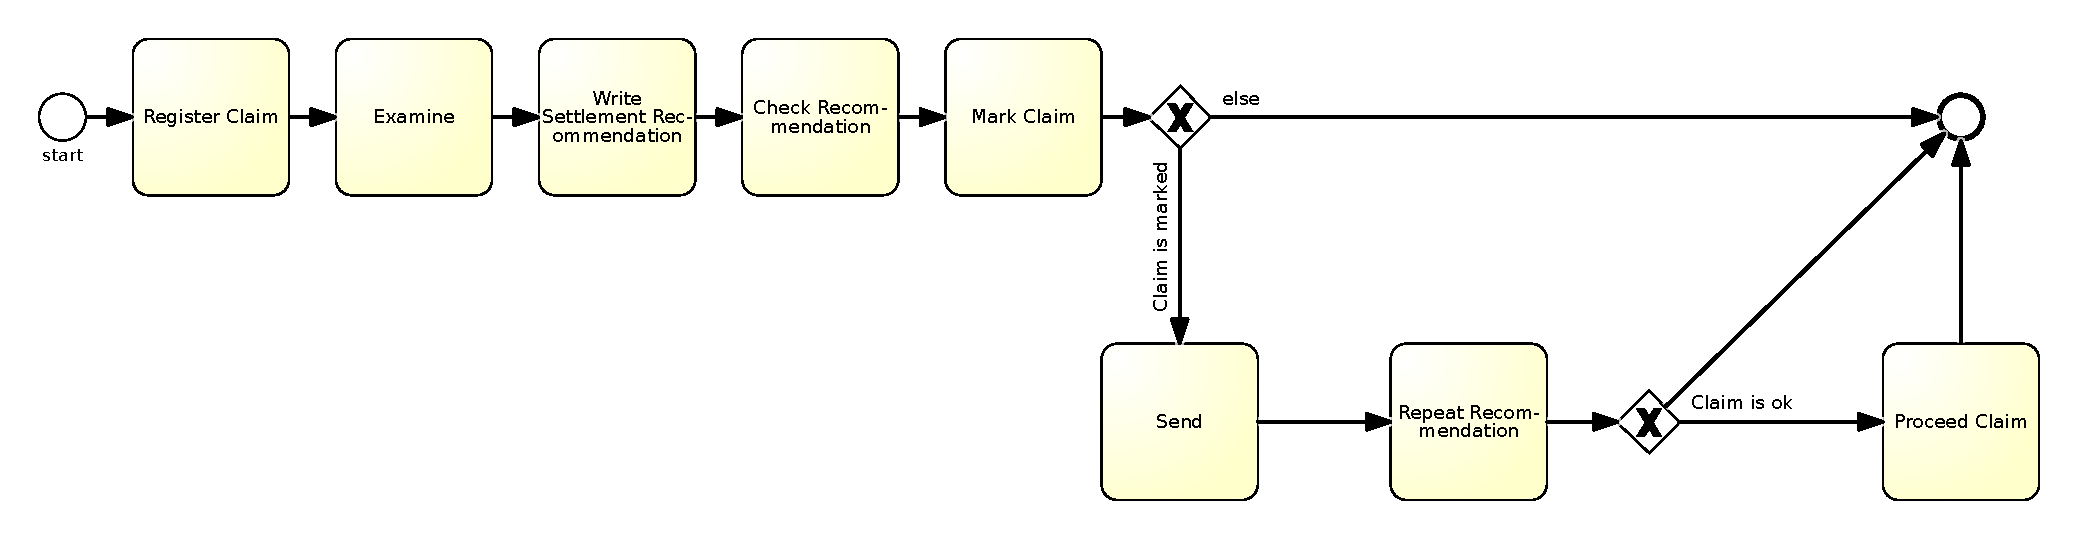
\includegraphics[width=\hsize]{./generated_bpmn/model9.pdf}
	\caption{BPMN diagram for process model 9 generated from spreadsheet-based model}
	\label{bpmn:generated_model9}
\end{figure}

\begin{figure}[H]
	\centering
	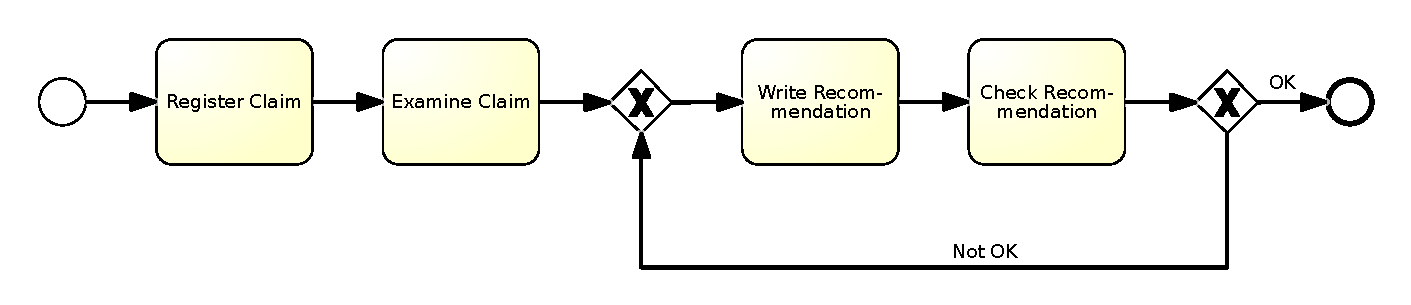
\includegraphics[width=\hsize]{./bpmn/model9.pdf}
	\caption{Hand-made BPMN diagram for process model 9}
	\label{bpmn:model9}
\end{figure}

\section{Model 10}
\begin{tcolorbox}[
	breakable,
	arc=0mm,
	left=1pt,
	right = 1pt,
	boxrule=0mm,
	colback = {white},
	]
	\texttt{\input{./models/model10.txt}}
\end{tcolorbox}
\captionof{textdesc}{Text description for model 10}
\label{txt:model10}

{\scriptsize
	\begin{longtable}{|p{0.03 \hsize}|p{0.25 \hsize}|p{0.15 \hsize}|p{0.2 \hsize}|p{0.1 \hsize}|p{0.1 \hsize}|}
		\hline
		Order & Activity & Condition & Who & Subprocess & Terminated.
		\\\hline\hline
		\csvreader[late after line=\\\hline]
		{./results/model10_intermediate_model.csv}
		{Order=\Order,Activity=\Activity,Condition=\Condition,Who=\Who,Subprocess=\Subprocess,Terminated=\Terminated}
		{\Order & \Activity & \Condition & \Who & \Subprocess & \Terminated}
		\caption{Spreadsheet-based description for process model 10}
		\label{csv:model10}
	\end{longtable}
}

\begin{figure}[H]
	\centering
	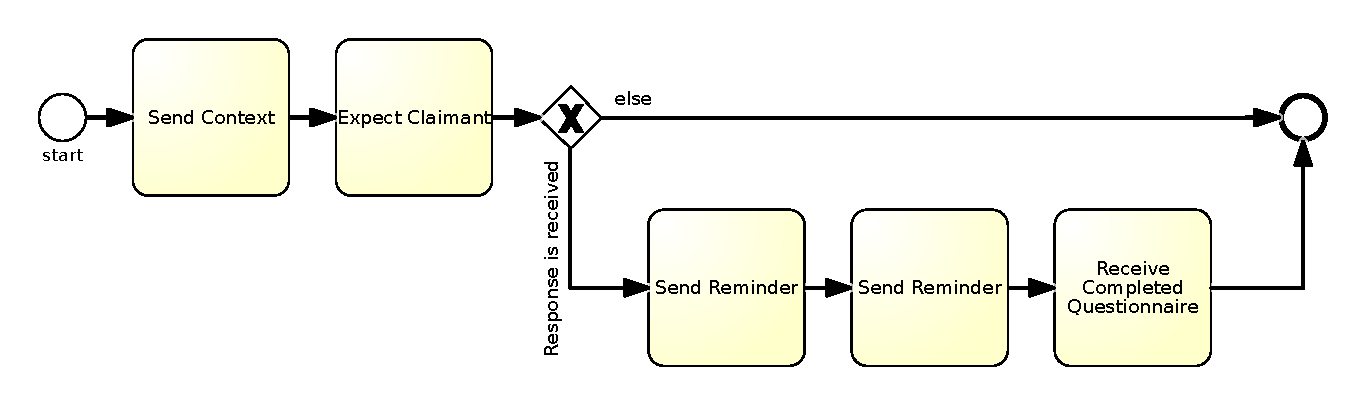
\includegraphics[width=\hsize]{./generated_bpmn/model10.pdf}
	\caption{BPMN diagram for process model 10 generated from spreadsheet-based model}
	\label{bpmn:generated_model10}
\end{figure}

\begin{figure}[H]
	\centering
	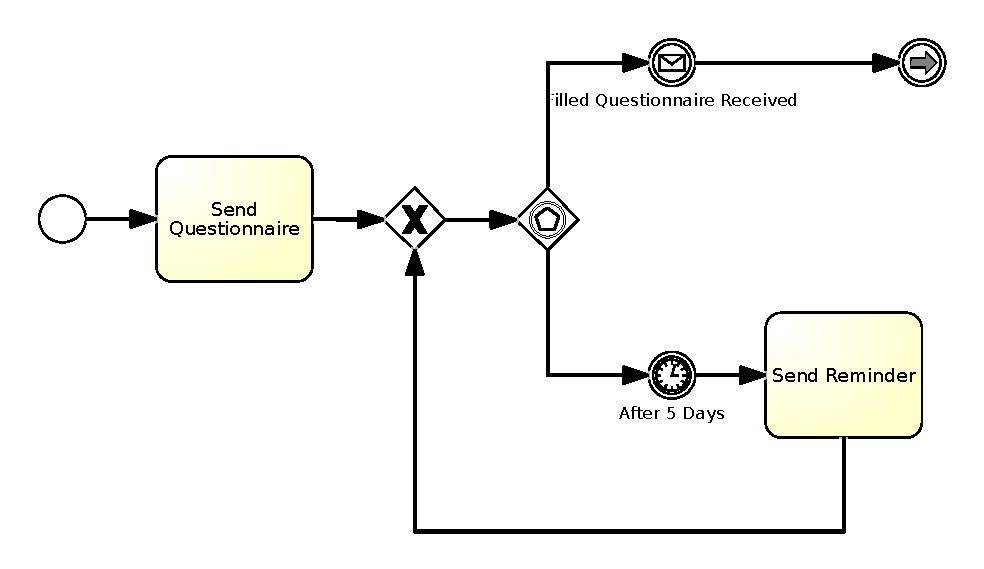
\includegraphics[width=\hsize]{./bpmn/model10.pdf}
	\caption{Hand-made BPMN diagram for process model 10}
	\label{bpmn:model10}
\end{figure}

\section{Model 11}
\begin{tcolorbox}[
	breakable,
	arc=0mm,
	left=1pt,
	right = 1pt,
	boxrule=0mm,
	colback = {white},
	]
	\texttt{\input{./models/model11.txt}}
\end{tcolorbox}
\captionof{textdesc}{Text description for model 11}
\label{txt:model11}

{\scriptsize
	\begin{longtable}{|p{0.03 \hsize}|p{0.25 \hsize}|p{0.15 \hsize}|p{0.2 \hsize}|p{0.1 \hsize}|p{0.1 \hsize}|}
		\hline
		Order & Activity & Condition & Who & Subprocess & Terminated.
		\\\hline\hline
		\csvreader[late after line=\\\hline]
		{./results/model11_intermediate_model.csv}
		{Order=\Order,Activity=\Activity,Condition=\Condition,Who=\Who,Subprocess=\Subprocess,Terminated=\Terminated}
		{\Order & \Activity & \Condition & \Who & \Subprocess & \Terminated}
		\caption{Spreadsheet-based description for process model 11}
		\label{csv:model11}
	\end{longtable}
}

\begin{figure}[H]
	\centering
	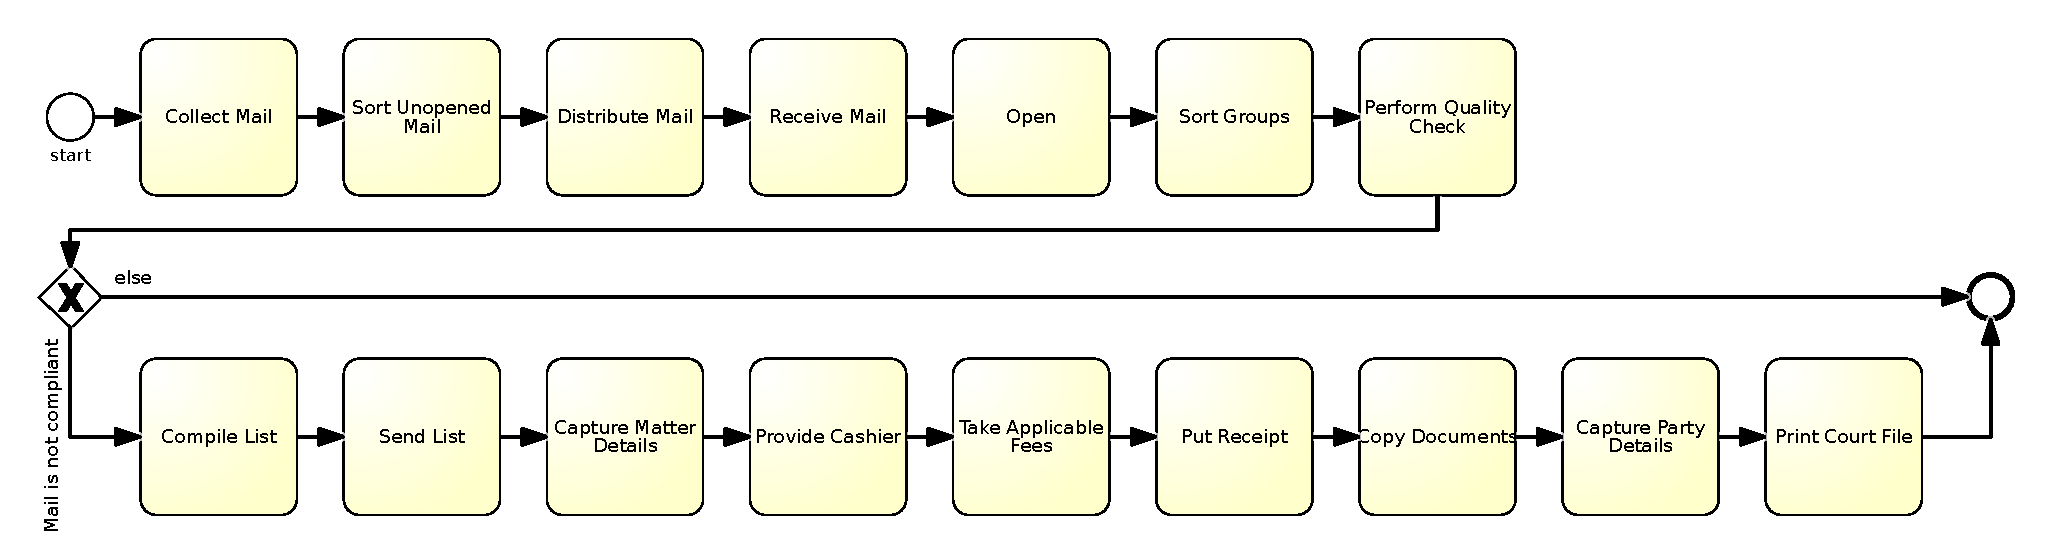
\includegraphics[width=\hsize]{./generated_bpmn/model11.pdf}
	\caption{BPMN diagram for process model 11 generated from spreadsheet-based model}
	\label{bpmn:generated_model11}
\end{figure}

\begin{figure}[H]
	\centering
	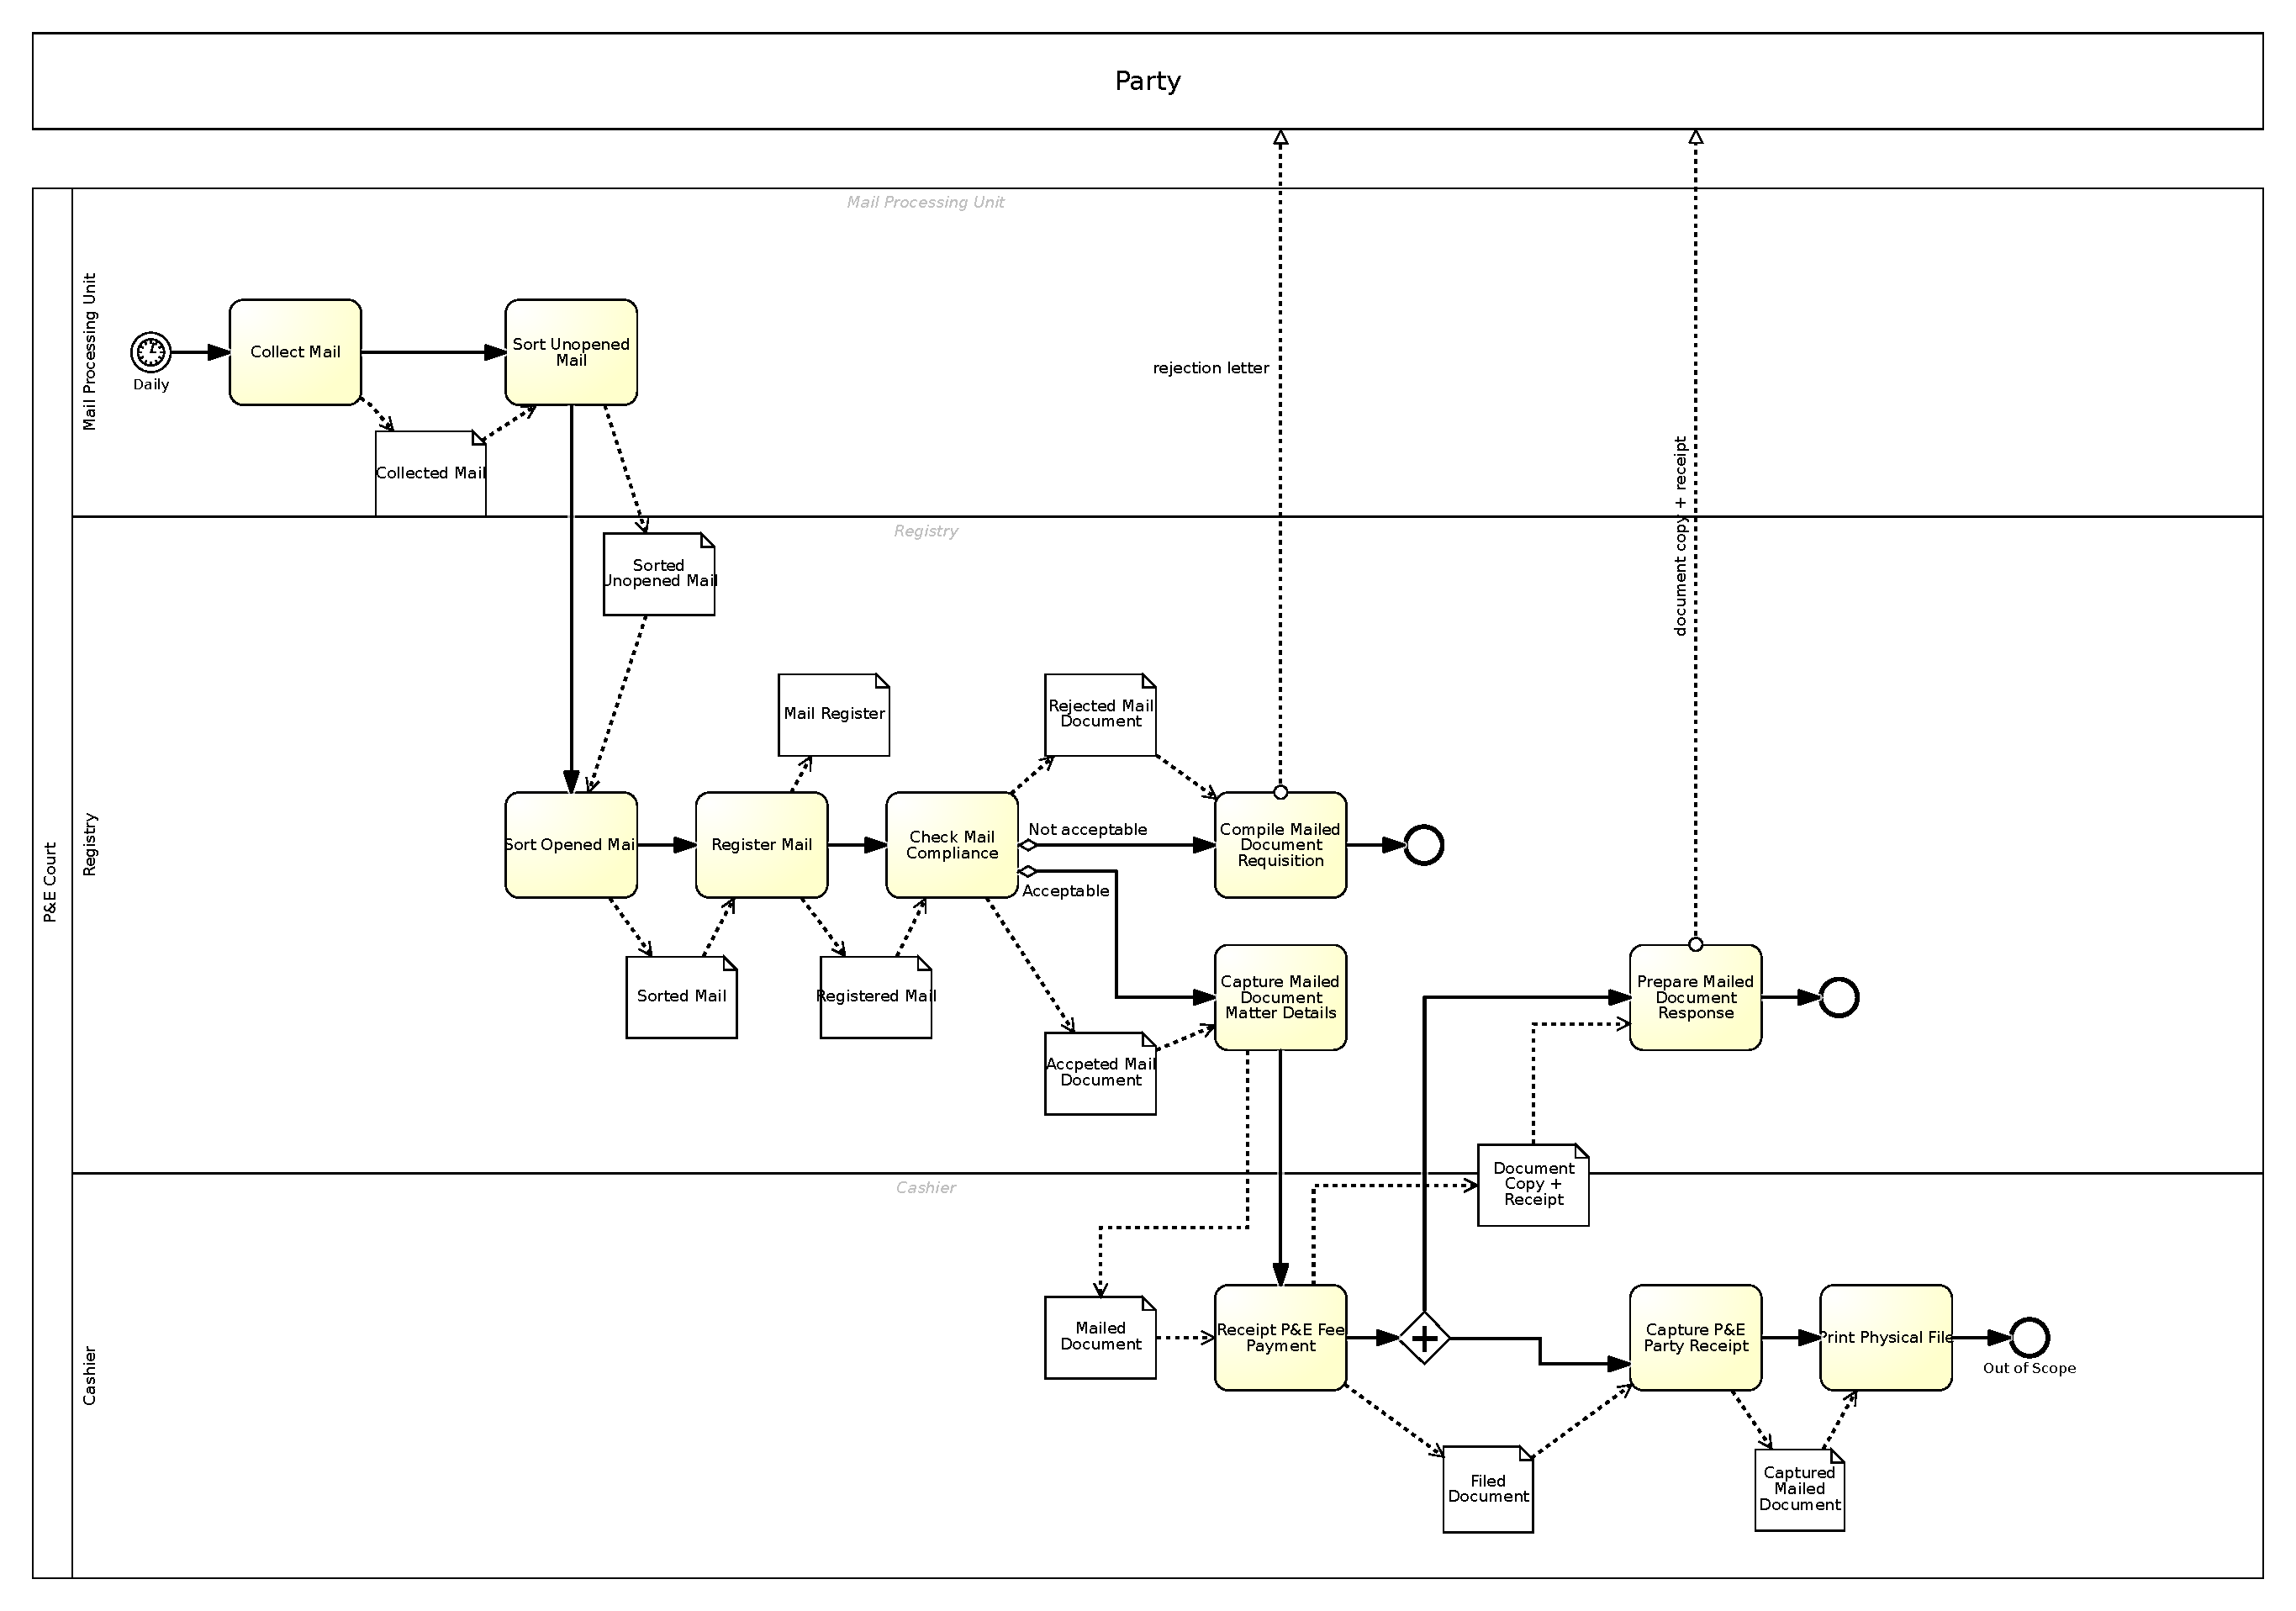
\includegraphics[width=\hsize]{./bpmn/model11.pdf}
	\caption{Hand-made BPMN diagram for process model 11}
	\label{bpmn:model11}
\end{figure}

\section{Model 12}
\begin{tcolorbox}[
	breakable,
	arc=0mm,
	left=1pt,
	right = 1pt,
	boxrule=0mm,
	colback = {white},
	]
	\texttt{\input{./models/model12.txt}}
\end{tcolorbox}
\captionof{textdesc}{Text description for model 12}
\label{txt:model12}

{\scriptsize
	\begin{longtable}{|p{0.03 \hsize}|p{0.25 \hsize}|p{0.15 \hsize}|p{0.2 \hsize}|p{0.1 \hsize}|p{0.1 \hsize}|}
		\hline
		Order & Activity & Condition & Who & Subprocess & Terminated.
		\\\hline\hline
		\csvreader[late after line=\\\hline]
		{./results/model12_intermediate_model.csv}
		{Order=\Order,Activity=\Activity,Condition=\Condition,Who=\Who,Subprocess=\Subprocess,Terminated=\Terminated}
		{\Order & \Activity & \Condition & \Who & \Subprocess & \Terminated}
		\caption{Spreadsheet-based description for process model 12}
		\label{csv:model12}
	\end{longtable}
}

\begin{figure}[H]
	\centering
	\includegraphics[width=\hsize]{./generated_bpmn/model12.pdf}
	\caption{BPMN diagram for process model 12 generated from spreadsheet-based model}
	\label{bpmn:generated_model12}
\end{figure}

\begin{figure}[H]
	\centering
	\includegraphics[width=\hsize]{./bpmn/model12.pdf}
	\caption{Hand-made BPMN diagram for process model 12}
	\label{bpmn:model12}
\end{figure}

\section{Model 13}
\begin{tcolorbox}[
	breakable,
	arc=0mm,
	left=1pt,
	right = 1pt,
	boxrule=0mm,
	colback = {white},
	]
	\texttt{\input{./models/model13.txt}}
\end{tcolorbox}
\captionof{textdesc}{Text description for model 13}
\label{txt:model13}

{\scriptsize
	\begin{longtable}{|p{0.03 \hsize}|p{0.25 \hsize}|p{0.15 \hsize}|p{0.2 \hsize}|p{0.1 \hsize}|p{0.1 \hsize}|}
		\hline
		Order & Activity & Condition & Who & Subprocess & Terminated.
		\\\hline\hline
		\csvreader[late after line=\\\hline]
		{./results/model13_intermediate_model.csv}
		{Order=\Order,Activity=\Activity,Condition=\Condition,Who=\Who,Subprocess=\Subprocess,Terminated=\Terminated}
		{\Order & \Activity & \Condition & \Who & \Subprocess & \Terminated}
		\caption{Spreadsheet-based description for process model 13}
		\label{csv:model13}
	\end{longtable}
}

\begin{figure}[H]
	\centering
	\includegraphics[width=\hsize]{./generated_bpmn/model13.pdf}
	\caption{BPMN diagram for process model 13 generated from spreadsheet-based model}
	\label{bpmn:generated_model13}
\end{figure}

\begin{figure}[H]
	\centering
	\includegraphics[width=\hsize]{./bpmn/model13.pdf}
	\caption{Hand-made BPMN diagram for process model 13}
	\label{bpmn:model13}
\end{figure}

\section{Model 14}
\begin{tcolorbox}[
	breakable,
	arc=0mm,
	left=1pt,
	right = 1pt,
	boxrule=0mm,
	colback = {white},
	]
	\texttt{\input{./models/model14.txt}}
\end{tcolorbox}
\captionof{textdesc}{Text description for model 14}
\label{txt:model14}

{\scriptsize
	\begin{longtable}{|p{0.03 \hsize}|p{0.25 \hsize}|p{0.15 \hsize}|p{0.2 \hsize}|p{0.1 \hsize}|p{0.1 \hsize}|}
		\hline
		Order & Activity & Condition & Who & Subprocess & Terminated.
		\\\hline\hline
		\csvreader[late after line=\\\hline]
		{./results/model14_intermediate_model.csv}
		{Order=\Order,Activity=\Activity,Condition=\Condition,Who=\Who,Subprocess=\Subprocess,Terminated=\Terminated}
		{\Order & \Activity & \Condition & \Who & \Subprocess & \Terminated}
		\caption{Spreadsheet-based description for process model 14}
		\label{csv:model14}
	\end{longtable}
}

\begin{figure}[H]
	\centering
	\includegraphics[width=0.95\textheight, angle=90]{./generated_bpmn/model14.pdf}
	\caption{BPMN diagram for process model 14 generated from spreadsheet-based model}
	\label{bpmn:generated_model14}
\end{figure}

\begin{figure}[H]
	\centering
	\includegraphics[width=0.95\textheight, angle=90]{./bpmn/model14.pdf}
	\caption{Hand-made BPMN diagram for process model 14}
	\label{bpmn:model14}
\end{figure}

\section{Model 15}
\begin{tcolorbox}[
	breakable,
	arc=0mm,
	left=1pt,
	right = 1pt,
	boxrule=0mm,
	colback = {white},
	]
	\texttt{\input{./models/model15.txt}}
\end{tcolorbox}
\captionof{textdesc}{Text description for model 15}
\label{txt:model15}

{\scriptsize
	\begin{longtable}{|p{0.03 \hsize}|p{0.25 \hsize}|p{0.15 \hsize}|p{0.2 \hsize}|p{0.1 \hsize}|p{0.1 \hsize}|}
		\hline
		Order & Activity & Condition & Who & Subprocess & Terminated.
		\\\hline\hline
		\csvreader[late after line=\\\hline]
		{./results/model15_intermediate_model.csv}
		{Order=\Order,Activity=\Activity,Condition=\Condition,Who=\Who,Subprocess=\Subprocess,Terminated=\Terminated}
		{\Order & \Activity & \Condition & \Who & \Subprocess & \Terminated}
		\caption{Spreadsheet-based description for process model 15}
		\label{csv:model15}
	\end{longtable}
}

\begin{figure}[H]
	\centering
	\includegraphics[width=\hsize]{./generated_bpmn/model15.pdf}
	\caption{BPMN diagram for process model 15 generated from spreadsheet-based model}
	\label{bpmn:generated_model15}
\end{figure}

\begin{figure}[H]
	\centering
	\includegraphics[scale=1.0]{./bpmn/model15.pdf}
	\caption{Hand-made BPMN diagram for process model 15}
	\label{bpmn:model15}
\end{figure}

\section{Model 16}
\begin{tcolorbox}[
	breakable,
	arc=0mm,
	left=1pt,
	right = 1pt,
	boxrule=0mm,
	colback = {white},
	]
	\texttt{\input{./models/model16.txt}}
\end{tcolorbox}
\captionof{textdesc}{Text description for model 16}
\label{txt:model16}

{\scriptsize
	\begin{longtable}{|p{0.03 \hsize}|p{0.25 \hsize}|p{0.15 \hsize}|p{0.2 \hsize}|p{0.1 \hsize}|p{0.1 \hsize}|}
		\hline
		Order & Activity & Condition & Who & Subprocess & Terminated.
		\\\hline\hline
		\csvreader[late after line=\\\hline]
		{./results/model16_intermediate_model.csv}
		{Order=\Order,Activity=\Activity,Condition=\Condition,Who=\Who,Subprocess=\Subprocess,Terminated=\Terminated}
		{\Order & \Activity & \Condition & \Who & \Subprocess & \Terminated}
		\caption{Spreadsheet-based description for process model 16}
		\label{csv:model16}
	\end{longtable}
}

\begin{figure}[H]
	\centering
	\includegraphics[width=\hsize]{./generated_bpmn/model16.pdf}
	\caption{BPMN diagram for process model 16 generated from spreadsheet-based model}
	\label{bpmn:generated_model16}
\end{figure}

\begin{figure}[H]
	\centering
	\includegraphics[scale=0.5]{./bpmn/model16.pdf}
	\caption{Hand-made BPMN diagram for process model 16}
	\label{bpmn:model16}
\end{figure}

\section{Model 17}
\begin{tcolorbox}[
	breakable,
	arc=0mm,
	left=1pt,
	right = 1pt,
	boxrule=0mm,
	colback = {white},
	]
	\texttt{\input{./models/model17.txt}}
\end{tcolorbox}
\captionof{textdesc}{Text description for model 17}
\label{txt:model17}

{\scriptsize
	\begin{longtable}{|p{0.03 \hsize}|p{0.25 \hsize}|p{0.15 \hsize}|p{0.2 \hsize}|p{0.1 \hsize}|p{0.1 \hsize}|}
		\hline
		Order & Activity & Condition & Who & Subprocess & Terminated.
		\\\hline\hline
		\csvreader[late after line=\\\hline]
		{./results/model17_intermediate_model.csv}
		{Order=\Order,Activity=\Activity,Condition=\Condition,Who=\Who,Subprocess=\Subprocess,Terminated=\Terminated}
		{\Order & \Activity & \Condition & \Who & \Subprocess & \Terminated}
		\caption{Spreadsheet-based description for process model 17}
		\label{csv:model17}
	\end{longtable}
}

\begin{figure}[H]
	\centering
	\includegraphics[width=\hsize]{./generated_bpmn/model17.pdf}
	\caption{BPMN diagram for process model 17 generated from spreadsheet-based model}
	\label{bpmn:generated_model17}
\end{figure}

\begin{figure}[H]
	\centering
	\includegraphics[width=\hsize]{./bpmn/model17.pdf}
	\caption{Hand-made BPMN diagram for process model 17}
	\label{bpmn:model17}
\end{figure}

\section{Model 18}
\begin{tcolorbox}[
	breakable,
	arc=0mm,
	left=1pt,
	right = 1pt,
	boxrule=0mm,
	colback = {white},
	]
	\texttt{\input{./models/model18.txt}}
\end{tcolorbox}
\captionof{textdesc}{Text description for model 18}
\label{txt:model18}

{\scriptsize
	\begin{longtable}{|p{0.03 \hsize}|p{0.25 \hsize}|p{0.15 \hsize}|p{0.2 \hsize}|p{0.1 \hsize}|p{0.1 \hsize}|}
		\hline
		Order & Activity & Condition & Who & Subprocess & Terminated.
		\\\hline\hline
		\csvreader[late after line=\\\hline]
		{./results/model18_intermediate_model.csv}
		{Order=\Order,Activity=\Activity,Condition=\Condition,Who=\Who,Subprocess=\Subprocess,Terminated=\Terminated}
		{\Order & \Activity & \Condition & \Who & \Subprocess & \Terminated}
		\caption{Spreadsheet-based description for process model 18}
		\label{csv:model18}
	\end{longtable}
}

\begin{figure}[H]
	\centering
	\includegraphics[width=\hsize]{./generated_bpmn/model18.pdf}
	\caption{BPMN diagram for process model 18 generated from spreadsheet-based model}
	\label{bpmn:generated_model18}
\end{figure}

\begin{figure}[H]
	\centering
	\includegraphics[width=\hsize]{./bpmn/model18.pdf}
	\caption{Hand-made BPMN diagram for process model 18}
	\label{bpmn:model18}
\end{figure}

\section{Model 19}
\begin{tcolorbox}[
	breakable,
	arc=0mm,
	left=1pt,
	right = 1pt,
	boxrule=0mm,
	colback = {white},
	]
	\texttt{\input{./models/model19.txt}}
\end{tcolorbox}
\captionof{textdesc}{Text description for model 19}
\label{txt:model19}
\newpage
{\scriptsize
	\begin{longtable}{|p{0.03 \hsize}|p{0.25 \hsize}|p{0.15 \hsize}|p{0.2 \hsize}|p{0.1 \hsize}|p{0.1 \hsize}|}
		\hline
		Order & Activity & Condition & Who & Subprocess & Terminated.
		\\\hline\hline
		\csvreader[late after line=\\\hline]
		{./results/model19_intermediate_model.csv}
		{Order=\Order,Activity=\Activity,Condition=\Condition,Who=\Who,Subprocess=\Subprocess,Terminated=\Terminated}
		{\Order & \Activity & \Condition & \Who & \Subprocess & \Terminated}
		\caption{Spreadsheet-based description for process model 19}
		\label{csv:model19}
	\end{longtable}
}

\begin{figure}[H]
	\centering
	\includegraphics[width=\hsize]{./bpmn/model19.pdf}
	\caption{Hand-made BPMN diagram for process model 19}
	\label{bpmn:model19}
\end{figure}

\begin{figure}[H]
	\centering
	\includegraphics[width=\hsize]{./generated_bpmn/model19.pdf}
	\caption{BPMN diagram for process model 19 generated from spreadsheet-based model}
	\label{bpmn:generated_model19}
\end{figure}

\section{Model 20}
\begin{tcolorbox}[
	breakable,
	arc=0mm,
	left=1pt,
	right = 1pt,
	boxrule=0mm,
	colback = {white},
	]
	\texttt{\input{./models/model20.txt}}
\end{tcolorbox}
\captionof{textdesc}{Text description for model 20}
\label{txt:model20}

{\scriptsize
	\begin{longtable}{|p{0.03 \hsize}|p{0.25 \hsize}|p{0.15 \hsize}|p{0.2 \hsize}|p{0.1 \hsize}|p{0.1 \hsize}|}
		\hline
		Order & Activity & Condition & Who & Subprocess & Terminated.
		\\\hline\hline
		\csvreader[late after line=\\\hline]
		{./results/model20_intermediate_model.csv}
		{Order=\Order,Activity=\Activity,Condition=\Condition,Who=\Who,Subprocess=\Subprocess,Terminated=\Terminated}
		{\Order & \Activity & \Condition & \Who & \Subprocess & \Terminated}
		\caption{Spreadsheet-based description for process model 20}
		\label{csv:model20}
	\end{longtable}
}

\begin{figure}[H]
	\centering
	\includegraphics[width=\hsize]{./generated_bpmn/model20.pdf}
	\caption{BPMN diagram for process model 20 generated from spreadsheet-based model}
	\label{bpmn:generated_model20}
\end{figure}

\begin{figure}[H]
	\centering
	\includegraphics[scale=0.7]{./bpmn/model20.pdf}
	\caption{Hand-made BPMN diagram for process model 20}
	\label{bpmn:model20}
\end{figure}

\section{Model 21}
\begin{tcolorbox}[
	breakable,
	arc=0mm,
	left=1pt,
	right = 1pt,
	boxrule=0mm,
	colback = {white},
	]
	\texttt{\input{./models/model21.txt}}
\end{tcolorbox}
\captionof{textdesc}{Text description for model 21}
\label{txt:model21}

{\scriptsize
	\begin{longtable}{|p{0.03 \hsize}|p{0.25 \hsize}|p{0.15 \hsize}|p{0.2 \hsize}|p{0.1 \hsize}|p{0.1 \hsize}|}
		\hline
		Order & Activity & Condition & Who & Subprocess & Terminated.
		\\\hline\hline
		\csvreader[late after line=\\\hline]
		{./results/model21_intermediate_model.csv}
		{Order=\Order,Activity=\Activity,Condition=\Condition,Who=\Who,Subprocess=\Subprocess,Terminated=\Terminated}
		{\Order & \Activity & \Condition & \Who & \Subprocess & \Terminated}
		\caption{Spreadsheet-based description for process model 21}
		\label{csv:model21}
	\end{longtable}
}

\begin{figure}[H]
	\centering
	\includegraphics[width=\hsize]{./generated_bpmn/model21.pdf}
	\caption{BPMN diagram for process model 21 generated from spreadsheet-based model}
	\label{bpmn:generated_model21}
\end{figure}

\begin{figure}[H]
	\centering
	\includegraphics[width=\hsize]{./bpmn/model21.pdf}
	\caption{Hand-made BPMN diagram for process model 21}
	\label{bpmn:model21}
\end{figure}

\section{Model 22}
\begin{tcolorbox}[
	breakable,
	arc=0mm,
	left=1pt,
	right = 1pt,
	boxrule=0mm,
	colback = {white},
	]
	\texttt{\input{./models/model22.txt}}
\end{tcolorbox}
\captionof{textdesc}{Text description for model 22}
\label{txt:model22}

{\scriptsize
	\begin{longtable}{|p{0.03 \hsize}|p{0.25 \hsize}|p{0.15 \hsize}|p{0.2 \hsize}|p{0.1 \hsize}|p{0.1 \hsize}|}
		\hline
		Order & Activity & Condition & Who & Subprocess & Terminated.
		\\\hline\hline
		\csvreader[late after line=\\\hline]
		{./results/model22_intermediate_model.csv}
		{Order=\Order,Activity=\Activity,Condition=\Condition,Who=\Who,Subprocess=\Subprocess,Terminated=\Terminated}
		{\Order & \Activity & \Condition & \Who & \Subprocess & \Terminated}
		\caption{Spreadsheet-based description for process model 22}
		\label{csv:model22}
	\end{longtable}
}

\begin{figure}[H]
	\centering
	\includegraphics[scale=0.4]{./generated_bpmn/model22.pdf}
	\caption{BPMN diagram for process model 22 generated from spreadsheet-based model}
	\label{bpmn:generated_model22}
\end{figure}

\begin{figure}[H]
	\centering
	\includegraphics[width=0.95\textheight, angle=90]{./bpmn/model22.pdf}
	\caption{Hand-made BPMN diagram for process model 22}
	\label{bpmn:model22}
\end{figure}

\section{Model 23}
\begin{tcolorbox}[
	breakable,
	arc=0mm,
	left=1pt,
	right = 1pt,
	boxrule=0mm,
	colback = {white},
	]
	\texttt{\input{./models/model23.txt}}
\end{tcolorbox}
\captionof{textdesc}{Text description for model 23}
\label{txt:model23}

{\scriptsize
	\begin{longtable}{|p{0.03 \hsize}|p{0.25 \hsize}|p{0.15 \hsize}|p{0.2 \hsize}|p{0.1 \hsize}|p{0.1 \hsize}|}
		\hline
		Order & Activity & Condition & Who & Subprocess & Terminated.
		\\\hline\hline
		\csvreader[late after line=\\\hline]
		{./results/model23_intermediate_model.csv}
		{Order=\Order,Activity=\Activity,Condition=\Condition,Who=\Who,Subprocess=\Subprocess,Terminated=\Terminated}
		{\Order & \Activity & \Condition & \Who & \Subprocess & \Terminated}
		\caption{Spreadsheet-based description for process model 23}
		\label{csv:model23}
	\end{longtable}
}

\begin{figure}[H]
	\centering
	\includegraphics[width=\hsize]{./generated_bpmn/model23.pdf}
	\caption{BPMN diagram for process model 23 generated from spreadsheet-based model}
	\label{bpmn:generated_model23}
\end{figure}

\begin{figure}[H]
	\centering
	\includegraphics[width=\hsize]{./bpmn/model23.pdf}
	\caption{Hand-made BPMN diagram for process model 23}
	\label{bpmn:model23}
\end{figure}

\section{Model 24}
\begin{tcolorbox}[
	breakable,
	arc=0mm,
	left=1pt,
	right = 1pt,
	boxrule=0mm,
	colback = {white},
	]
	\texttt{\input{./models/model24.txt}}
\end{tcolorbox}
\captionof{textdesc}{Text description for model 24}
\label{txt:model24}

{\scriptsize
	\begin{longtable}{|p{0.03 \hsize}|p{0.25 \hsize}|p{0.15 \hsize}|p{0.2 \hsize}|p{0.1 \hsize}|p{0.1 \hsize}|}
		\hline
		Order & Activity & Condition & Who & Subprocess & Terminated.
		\\\hline\hline
		\csvreader[late after line=\\\hline]
		{./results/model24_intermediate_model.csv}
		{Order=\Order,Activity=\Activity,Condition=\Condition,Who=\Who,Subprocess=\Subprocess,Terminated=\Terminated}
		{\Order & \Activity & \Condition & \Who & \Subprocess & \Terminated}
		\caption{Spreadsheet-based description for process model 24}
		\label{csv:model24}
	\end{longtable}
}

\begin{figure}[H]
	\centering
	\includegraphics[width=\hsize]{./generated_bpmn/model24.pdf}
	\caption{BPMN diagram for process model 24 generated from spreadsheet-based model}
	\label{bpmn:generated_model24}
\end{figure}

\begin{figure}[H]
	\centering
	\includegraphics[width=\hsize]{./bpmn/model24.pdf}
	\caption{Hand-made BPMN diagram for process model 24}
	\label{bpmn:model24}
\end{figure}

\section{Model 25}
\begin{tcolorbox}[
	breakable,
	arc=0mm,
	left=1pt,
	right = 1pt,
	boxrule=0mm,
	colback = {white},
	]
	\texttt{\input{./models/model25.txt}}
\end{tcolorbox}
\captionof{textdesc}{Text description for model 25}
\label{txt:model25}
\newpage
{\scriptsize
	\begin{longtable}{|p{0.03 \hsize}|p{0.25 \hsize}|p{0.15 \hsize}|p{0.2 \hsize}|p{0.1 \hsize}|p{0.1 \hsize}|}
		\hline
		Order & Activity & Condition & Who & Subprocess & Terminated.
		\\\hline\hline
		\csvreader[late after line=\\\hline]
		{./results/model25_intermediate_model.csv}
		{Order=\Order,Activity=\Activity,Condition=\Condition,Who=\Who,Subprocess=\Subprocess,Terminated=\Terminated}
		{\Order & \Activity & \Condition & \Who & \Subprocess & \Terminated}
		\caption{Spreadsheet-based description for process model 25}
		\label{csv:model25}
	\end{longtable}
}

\begin{figure}[H]
	\centering
	\includegraphics[width=\hsize]{./generated_bpmn/model25.pdf}
	\caption{BPMN diagram for process model 25 generated from spreadsheet-based model}
	\label{bpmn:generated_model25}
\end{figure}

\begin{figure}[H]
	\centering
	\includegraphics[width=\hsize]{./bpmn/model25.pdf}
	\caption{Hand-made BPMN diagram for process model 25}
	\label{bpmn:model25}
\end{figure}

\section{Model 26}
\begin{tcolorbox}[
	breakable,
	arc=0mm,
	left=1pt,
	right = 1pt,
	boxrule=0mm,
	colback = {white},
	]
	\texttt{\input{./models/model26.txt}}
\end{tcolorbox}
\captionof{textdesc}{Text description for model 26}
\label{txt:model26}

{\scriptsize
	\begin{longtable}{|p{0.03 \hsize}|p{0.25 \hsize}|p{0.15 \hsize}|p{0.2 \hsize}|p{0.1 \hsize}|p{0.1 \hsize}|}
		\hline
		Order & Activity & Condition & Who & Subprocess & Terminated.
		\\\hline\hline
		\csvreader[late after line=\\\hline]
		{./results/model26_intermediate_model.csv}
		{Order=\Order,Activity=\Activity,Condition=\Condition,Who=\Who,Subprocess=\Subprocess,Terminated=\Terminated}
		{\Order & \Activity & \Condition & \Who & \Subprocess & \Terminated}
		\caption{Spreadsheet-based description for process model 26}
		\label{csv:model26}
	\end{longtable}
}

\begin{figure}[H]
	\centering
	\includegraphics[width=\hsize]{./generated_bpmn/model26.pdf}
	\caption{BPMN diagram for process model 26 generated from spreadsheet-based model}
	\label{bpmn:generated_model26}
\end{figure}

\begin{figure}[H]
	\centering
	\includegraphics[width=\hsize]{./bpmn/model26.pdf}
	\caption{Hand-made BPMN diagram for process model 26}
	\label{bpmn:model26}
\end{figure}

\section{Model 27}
\begin{tcolorbox}[
	breakable,
	arc=0mm,
	left=1pt,
	right = 1pt,
	boxrule=0mm,
	colback = {white},
	]
	\texttt{\input{./models/model27.txt}}
\end{tcolorbox}
\captionof{textdesc}{Text description for model 27}
\label{txt:model27}

{\scriptsize
	\begin{longtable}{|p{0.03 \hsize}|p{0.25 \hsize}|p{0.15 \hsize}|p{0.2 \hsize}|p{0.1 \hsize}|p{0.1 \hsize}|}
		\hline
		Order & Activity & Condition & Who & Subprocess & Terminated.
		\\\hline\hline
		\csvreader[late after line=\\\hline]
		{./results/model27_intermediate_model.csv}
		{Order=\Order,Activity=\Activity,Condition=\Condition,Who=\Who,Subprocess=\Subprocess,Terminated=\Terminated}
		{\Order & \Activity & \Condition & \Who & \Subprocess & \Terminated}
		\caption{Spreadsheet-based description for process model 27}
		\label{csv:model27}
	\end{longtable}
}

\begin{figure}[H]
	\centering
	\includegraphics[width=\hsize]{./generated_bpmn/model27.pdf}
	\caption{BPMN diagram for process model 27 generated from spreadsheet-based model}
	\label{bpmn:generated_model27}
\end{figure}

\begin{figure}[H]
	\centering
	\includegraphics[width=\hsize]{./bpmn/model27.pdf}
	\caption{Hand-made BPMN diagram for process model 27}
	\label{bpmn:model27}
\end{figure}

\section{Model 28}
\begin{tcolorbox}[
	breakable,
	arc=0mm,
	left=1pt,
	right = 1pt,
	boxrule=0mm,
	colback = {white},
	]
	\texttt{\input{./models/model28.txt}}
\end{tcolorbox}
\captionof{textdesc}{Text description for model 28}
\label{txt:model28}

{\scriptsize
	\begin{longtable}{|p{0.03 \hsize}|p{0.25 \hsize}|p{0.15 \hsize}|p{0.2 \hsize}|p{0.1 \hsize}|p{0.1 \hsize}|}
		\hline
		Order & Activity & Condition & Who & Subprocess & Terminated.
		\\\hline\hline
		\csvreader[late after line=\\\hline]
		{./results/model28_intermediate_model.csv}
		{Order=\Order,Activity=\Activity,Condition=\Condition,Who=\Who,Subprocess=\Subprocess,Terminated=\Terminated}
		{\Order & \Activity & \Condition & \Who & \Subprocess & \Terminated}
		\caption{Spreadsheet-based description for process model 28}
		\label{csv:model28}
	\end{longtable}
}

\begin{figure}[H]
	\centering
	\includegraphics[width=\hsize]{./generated_bpmn/model28.pdf}
	\caption{BPMN diagram for process model 28 generated from spreadsheet-based model}
	\label{bpmn:generated_model28}
\end{figure}

\begin{figure}[H]
	\centering
	\includegraphics[width=\hsize]{./bpmn/model28.pdf}
	\caption{Hand-made BPMN diagram for process model 28}
	\label{bpmn:model28}
\end{figure}

\section{Model 29}
\begin{tcolorbox}[
	breakable,
	arc=0mm,
	left=1pt,
	right = 1pt,
	boxrule=0mm,
	colback = {white},
	]
	\texttt{\input{./models/model29.txt}}
\end{tcolorbox}
\captionof{textdesc}{Text description for model 29}
\label{txt:model29}

{\scriptsize
	\begin{longtable}{|p{0.03 \hsize}|p{0.25 \hsize}|p{0.15 \hsize}|p{0.2 \hsize}|p{0.1 \hsize}|p{0.1 \hsize}|}
		\hline
		Order & Activity & Condition & Who & Subprocess & Terminated.
		\\\hline\hline
		\csvreader[late after line=\\\hline]
		{./results/model29_intermediate_model.csv}
		{Order=\Order,Activity=\Activity,Condition=\Condition,Who=\Who,Subprocess=\Subprocess,Terminated=\Terminated}
		{\Order & \Activity & \Condition & \Who & \Subprocess & \Terminated}
		\caption{Spreadsheet-based description for process model 29}
		\label{csv:model29}
	\end{longtable}
}

\begin{figure}[H]
	\centering
	\includegraphics[width=\hsize]{./generated_bpmn/model29.pdf}
	\caption{BPMN diagram for process model 29 generated from spreadsheet-based model}
	\label{bpmn:generated_model29}
\end{figure}

\begin{figure}[H]
	\centering
	\includegraphics[width=\hsize]{./bpmn/model29.pdf}
	\caption{Hand-made BPMN diagram for process model 29}
	\label{bpmn:model29}
\end{figure}

\section{Model 30}
\begin{tcolorbox}[
	breakable,
	arc=0mm,
	left=1pt,
	right = 1pt,
	boxrule=0mm,
	colback = {white},
	]
	\texttt{\input{./models/model30.txt}}
\end{tcolorbox}
\captionof{textdesc}{Text description for model 30}
\label{txt:model30}

{\scriptsize
	\begin{longtable}{|p{0.03 \hsize}|p{0.25 \hsize}|p{0.15 \hsize}|p{0.2 \hsize}|p{0.1 \hsize}|p{0.1 \hsize}|}
		\hline
		Order & Activity & Condition & Who & Subprocess & Terminated.
		\\\hline\hline
		\csvreader[late after line=\\\hline]
		{./results/model30_intermediate_model.csv}
		{Order=\Order,Activity=\Activity,Condition=\Condition,Who=\Who,Subprocess=\Subprocess,Terminated=\Terminated}
		{\Order & \Activity & \Condition & \Who & \Subprocess & \Terminated}
		\caption{Spreadsheet-based description for process model 30}
		\label{csv:model30}
	\end{longtable}
}

\begin{figure}[H]
	\centering
	\includegraphics[width=\hsize]{./generated_bpmn/model30.pdf}
	\caption{BPMN diagram for process model 30 generated from spreadsheet-based model}
	\label{bpmn:generated_model30}
\end{figure}

\begin{figure}[H]
	\centering
	\includegraphics[width=\hsize]{./bpmn/model30.pdf}
	\caption{Hand-made BPMN diagram for process model 30}
	\label{bpmn:model30}
\end{figure}

\section{Model 31}
\begin{tcolorbox}[
	breakable,
	arc=0mm,
	left=1pt,
	right = 1pt,
	boxrule=0mm,
	colback = {white},
	]
	\texttt{\input{./models/model31.txt}}
\end{tcolorbox}
\captionof{textdesc}{Text description for model 31}
\label{txt:model31}

{\scriptsize
	\begin{longtable}{|p{0.03 \hsize}|p{0.25 \hsize}|p{0.15 \hsize}|p{0.2 \hsize}|p{0.1 \hsize}|p{0.1 \hsize}|}
		\hline
		Order & Activity & Condition & Who & Subprocess & Terminated.
		\\\hline\hline
		\csvreader[late after line=\\\hline]
		{./results/model31_intermediate_model.csv}
		{Order=\Order,Activity=\Activity,Condition=\Condition,Who=\Who,Subprocess=\Subprocess,Terminated=\Terminated}
		{\Order & \Activity & \Condition & \Who & \Subprocess & \Terminated}
		\caption{Spreadsheet-based description for process model 31}
		\label{csv:model31}
	\end{longtable}
}

\begin{figure}[H]
	\centering
	\includegraphics[width=\hsize]{./generated_bpmn/model31.pdf}
	\caption{BPMN diagram for process model 31 generated from spreadsheet-based model}
	\label{bpmn:generated_model31}
\end{figure}

\begin{figure}[H]
	\centering
	\includegraphics[width=\hsize]{./bpmn/model31.pdf}
	\caption{Hand-made BPMN diagram for process model 31}
	\label{bpmn:model31}
\end{figure}

\section{Model 32}
\begin{tcolorbox}[
	breakable,
	arc=0mm,
	left=1pt,
	right = 1pt,
	boxrule=0mm,
	colback = {white},
	]
	\texttt{\input{./models/model32.txt}}
\end{tcolorbox}
\captionof{textdesc}{Text description for model 32}
\label{txt:model32}

{\scriptsize
	\begin{longtable}{|p{0.03 \hsize}|p{0.25 \hsize}|p{0.15 \hsize}|p{0.2 \hsize}|p{0.1 \hsize}|p{0.1 \hsize}|}
		\hline
		Order & Activity & Condition & Who & Subprocess & Terminated.
		\\\hline\hline
		\csvreader[late after line=\\\hline]
		{./results/model32_intermediate_model.csv}
		{Order=\Order,Activity=\Activity,Condition=\Condition,Who=\Who,Subprocess=\Subprocess,Terminated=\Terminated}
		{\Order & \Activity & \Condition & \Who & \Subprocess & \Terminated}
		\caption{Spreadsheet-based description for process model 32}
		\label{csv:model32}
	\end{longtable}
}

\begin{figure}[H]
	\centering
	\includegraphics[width=\hsize]{./generated_bpmn/model32.pdf}
	\caption{BPMN diagram for process model 32 generated from spreadsheet-based model}
	\label{bpmn:generated_model32}
\end{figure}

\begin{figure}[H]
	\centering
	\includegraphics[width=0.95\textheight, angle=90]{./bpmn/model32.pdf}
	\caption{Hand-made BPMN diagram for process model 32}
	\label{bpmn:model32}
\end{figure}
\chapter{Dependency tags list}
\label{cha:dependencies-list}
Full list of dependency tags used in SpaCy parser.
\begin{itemize}
	\item acl -- finite and non-finite clausal modifier,
	\item acomp -- adjectival complement,
	\item advcl -- adverbial clause modifier,
	\item advmod -- adverbial modifier,
	\item agent -- agent,
	\item amod -- adjectival modifier,
	\item appos -- appositional modifier,
	\item attr -- attribute,
	\item aux -- auxiliary,
	\item auxpass -- passive auxiliary,
	\item case -- case marker,
	\item cc -- coordinating conjunction,
	\item ccomp -- clausal complement,
	\item complm -- complementizer,
	\item compound -- compound nouns/numbers,
	\item conj -- conjunct,
	\item csubj -- clausal subject,
	\item csubjpass -- clausal passive subject,
	\item dative -- dative,
	\item dep -- unclassified dependent,
	\item det -- determiner,
	\item dobj -- direct object,
	\item expl -- expletive,
	\item hmod -- modifier in hyphenation,
	\item hyph -- hyphen,
	\item infmod -- infinitival modifier,
	\item intj -- interjection,
	\item iobj -- indirect object,
	\item mark -- maker,
	\item meta -- meta modifier,
	\item neg -- negation modifier,
	\item nmod -- modifier of nominal,
	\item nn -- noun compound modifier,
	\item npadvmod -- noun phrase as adverbial modifier,
	\item nsubj -- nominal subject,
	\item nsubjpass -- nominal passive subject,
	\item num -- numeric modifier,
	\item number -- number compound modifier,
	\item nummod -- numeric modifiers,
	\item oprd -- object predicate,
	\item parataxis -- parenthetical modifier,
	\item partmod -- participial modifier,
	\item pcomp -- complement of a preposition,
	\item pobj -- object of a preposition,
	\item poss -- possession modifier,
	\item possesive -- possessive modifier,
	\item preconj -- pre-correlative conjunction,
	\item prep -- prepositional modifier,
	\item prt -- particle,
	\item punct -- punctuation,
	\item quantmod -- quantifier phrase modifier,
	\item relcl -- relative clause modifiers,
	\item root -- root,
	\item xcomp -- open clausal complement.
\end{itemize}
\chapter{Keywords list}
\label{cha:keywords-list}
\begin{table}[h]
	\centering
	\makebox[0pt][c]{\parbox{\hsize}{
		\begin{minipage}[h]{0.45\hsize}
			\begin{tabularx}{\textwidth}{|l|X|}
				\hline
				Keyword & Type\\
				\hline
				\hline
				if & conditional\\
				\hline
				whether & conditional\\
				\hline
				while & parallel\\
				\hline
				otherwise & default flow\\
				\hline
			\end{tabularx}
			\caption{Keywords used during gateway keywords search}
			\label{table:gateway-keywords}
		\end{minipage}
		\hfill
		\begin{minipage}[h]{0.45\hsize}
			\begin{tabularx}{\textwidth}{|X|}
				\hline
				Keyword\\
				\hline
				\hline
				atm\\
				\hline
				crm\\
				\hline
				crs\\
				\hline
				office\\
				\hline
				provisioning\\
				\hline
				secretary\\
				\hline
				support\\
				\hline
			\end{tabularx}
			\caption{Participant keywords used during semantic analysis of participants}
			\label{table:participants-keywords}
		\end{minipage}
	}}
\end{table}

\begin{table}[h]
	\begin{tabular}{|p{0.2 \hsize}|p{0.8 \hsize}|}
		\hline
		Hypernym & Definition\\
		\hline
		\hline
		facility & A building or place that provides a particular service or is used for a particular industry\\
		\hline
		group & Any number of entities (members) considered as a unit\\
		\hline
		organization & 1. A group of people who work together 2. The persons (or committees or departments etc.) who make up a body for the purpose of administering something\\
		\hline
		person & A human being\\
		\hline
		service & A company or agency that performs a public service\\
		\hline
		system & Instrumentality that combines interrelated interacting artifacts designed to work as a coherent entity\\
		\hline
	\end{tabular}
	\caption{Participants hypernyms used during semantic analysis of participants. Definitions taken from WordNet database.}
	\label{table:participants-hypernyms}
\end{table}

\begin{table}[h]
	\centering
	\makebox[0pt][c]{\parbox{\hsize}{
			\begin{minipage}[h]{0.45\hsize}
				\begin{tabularx}{\textwidth}{|X|}
					\hline
					Verb\\
					\hline
					\hline
					achieve\\
					\hline
					base\\
					\hline
					exist\\
					\hline
					know\\
					\hline
					make\\
					\hline
					need\\
					\hline
				\end{tabularx}
				\caption{Ignorable verbs list}
				\label{table:ignorable-verbs}
			\end{minipage}
			\hfill
			\begin{minipage}[h]{0.45\hsize}
				\begin{tabularx}{\textwidth}{|X|}
					\hline
					Verb\\
					\hline
					\hline
					be\\
					\hline
					can\\
					\hline
					do\\
					\hline
					go\\
					\hline
					have\\
					\hline
				\end{tabularx}
				\caption{Replaceable verbs list}
				\label{table:replaceable-verbs}
			\end{minipage}
	}}
\end{table}
\chapter{BPMN Python}
\label{cha:bpmn-python}
\section{Project description}
The \emph{bpmn\_python} package provide means to represent BPMN diagram as an object during program execution. The main functionalities of this package is an import and export of BPMN diagram from XML files (compatible with official BPMN 2.0 XML Schema). Handling thee spreadsheet-based model descriptions is still in early stage of development, but it is able to work with basic examples. In addition, this library provides methods to manually create a simple BPMN process by making a Python script and also implements a set of diagram complexity metrics from article~\cite{kluza-metrics}.
\section{Manual generation of BPMN diagram}
This section shows a simple example of how to create a BPMN diagram using \emph{bpmn\_python}. This example is taken form package wiki\footnote{\url{https://github.com/KrzyHonk/bpmn-python/wiki}}. Current version of \emph{bpmn\_python} allows the user to add basic BPMN elemenst, such as start, stop events, tasks, collapsed sub-processes or gateways (inclusive, exclusive, parallel) to BPMN diagram.\\
Firs, it is required to import the script with \texttt{\emph{BPMNDiagramGraph}} class:
\begin{lstlisting}[language=python]
import bpmn_python.bpmn_diagram_rep as diagram
\end{lstlisting}
Then, we can create a BPMNDiagramGraph object:
\begin{lstlisting}[language=python]
bpmn_graph = diagram.BPMNDiagramGraph()
bpmn_graph.create_new_diagram_graph(diagram_name="diagram1")
\end{lstlisting}
Using \texttt{\emph{add\_start\_event\_to\_diagram}} and \texttt{\emph{add\_task\_to\_diagram}}, we can create a new start event and task. Then, we have to connect those elements with sequence flow.\\
User is allowed to change few attributes of new elements - for each element created in this example a name will be given (by default name is an empty string).\\
Notice that all of the methods used to add new elements into diagram returns two objects - a string representing an ID of a new element and a reference to object representing this element. Since this example requires only an ID of element, we skip the object reference using anonymous variable (denoted by \_).
\begin{lstlisting}[language=python]
[start_id, _] = bpmn_graph.add_start_event_to_diagram(start_event_name="start_event")
[task1_id, _] = bpmn_graph.add_task_to_diagram(task_name="task1")
bpmn_graph.add_sequence_flow_to_diagram(start_id, task1_id, "start_to_one")
\end{lstlisting}
Now we can create an exclusive gateway (fork and join element) with two tasks:
\begin{lstlisting}[language=python]
[exclusive_gate_fork_id, _] = bpmn_graph.add_exclusive_gateway_to_diagram(gateway_name="exclusive_gate_fork")
[task1_ex_id, _] = bpmn_graph.add_task_to_diagram(task_name="task1_ex")
[task2_ex_id, _] = bpmn_graph.add_task_to_diagram(task_name="task2_ex")
[exclusive_gate_join_id, _] = bpmn_graph.add_exclusive_gateway_to_diagram(gateway_name="exclusive_gate_join")

bpmn_graph.add_sequence_flow_to_diagram(task1_id, exclusive_gate_fork_id, "one_to_ex_fork")
bpmn_graph.add_sequence_flow_to_diagram(exclusive_gate_fork_id, task1_ex_id, "ex_fork_to_ex_one")
bpmn_graph.add_sequence_flow_to_diagram(exclusive_gate_fork_id, task2_ex_id, "ex_fork_to_ex_two")
bpmn_graph.add_sequence_flow_to_diagram(task1_ex_id, exclusive_gate_join_id, "ex_one_to_ex_join")
bpmn_graph.add_sequence_flow_to_diagram(task2_ex_id, exclusive_gate_join_id, "ex_two_to_ex_join")
\end{lstlisting}

And finally, add second task and end event:
\begin{lstlisting}[language=python]
[task2_id, _] = bpmn_graph.add_task_to_diagram(task_name="task2")
[end_id, _] = bpmn_graph.add_end_event_to_diagram(end_event_name="end_event")
bpmn_graph.add_sequence_flow_to_diagram(exclusive_gate_join_id, task2_id, "ex_join_to_two")
bpmn_graph.add_sequence_flow_to_diagram(task2_id, end_id, "two_to_end")
\end{lstlisting}
Figure~\ref{fig:manual_gen_example} presents a visualization of created BPMN diagram.
\begin{figure}[H]
	\centering
	\includegraphics[scale=0.6]{./images/manually_gen_example.pdf}
	\caption{BPMN diagram manually created using \emph{bpmn\_python} package}
	\label{fig:manual_gen_example}
\end{figure}


%\chapter{Code listings}
\label{cha:listings}
\section{Participant extraction}
\begin{lstlisting}[language=Python, caption={Participant extraction function listing}, label={lst:participant_extraction}]
def extract_participants(sentence) -> List[Participant]:
  tmp_output = []
  output = []
  for word in sentence:
    if word.dep_ in ("nsubj", "nsubjpass"):
      participant = Participant(participant_token=word)
      if word.pos_ == "pron":
        participant.set_pronoun(True)
      tmp_output.append(participant)
    elif word.dep_ == "agent":
      for child in word.children:
        if child.dep_ == "pobj":
          participant = Participant(participant_token=child)
          if child.pos_ == "pron":
            participant.set_pronoun(True)
          tmp_output.append(participant)
  
  # Check if possible participant is a part of conjunction
  for word in sentence:
    if word.dep_ == "conj":
      for child in word.children:
      if child.dep_ in ("pobj", "dobj", "iobj", "attr"):
        participant = Participant(participant_token=child)
        if child.pos_ == "pron":
          participant.set_pronoun(True)
        tmp_output.append(participant)
  
  # Check if Participant is an acceptable entity
  for participant in tmp_output:
    participant_text = participant.get_participant_token().text
    
    insert_flag = False
    # Check whether participant is a pronoun
    if participant.is_pronoun():
      insert_flag = True
    
    if insert_flag is False:
    # Analyze participant hypernyms, in search for one of base keywords
      insert_flag = analyze_participants_hypernyms(participant_text,
      participants_hypernyms)
    
    if insert_flag is False:
      # Check if participant is one of keywords
      insert_flag = validate_participant(participant_text,
      participant_keywords_list)
    if insert_flag:
      output.append(participant)
  
  return output
\end{lstlisting}

\section{Subject-verb-object extraction}
\begin{lstlisting}[language=Python, caption={Subject-Verb-Object extraction function listing}, label={lst:svo_extraction}]
def extract_svo_constructs(sentence: Span,
participants: List[Participant]) -> List[SvoConstruct]:
  tmp_output = []
  root = sentence.root
  nsubj_list = dep.find_tokens_with_dependencies(root, ["nsubj"])
  nsubjpass_list = dep.find_tokens_with_dependencies(root, ["nsubjpass"])
  if len(nsubj_list) > 0:
    for token in nsubj_list:
      subject = token
      verb = subject.head
      output_obj = find_token_in_ancestors(verb,
      ("dobj", "iobj", "pobj", "attr"))
      if subject is not None and verb is not None:
        svo = SvoConstruct(subject=subject, 
          verb=verb, new_object=output_obj, position=verb.i)
        if len(tmp_output) > 0:
          if check_if_svo_is_unique(svo, tmp_output):
            tmp_output.append(svo)
        else:
          tmp_output.append(svo)
    
  if len(nsubjpass_list) > 0:
    for token in nsubjpass_list:
      subject = token
      verb = subject.head
      if subject is not None and verb is not None:
        svo = SvoConstruct(subject=subject, 
          verb=verb, position=verb.i)
        if len(tmp_output) > 0:
          if check_if_svo_is_unique(svo, tmp_output):
            tmp_output.append(svo)
        else:
        tmp_output.append(svo)
  
  # Check if conjunction exists in sentence and extract possible SVO
  for word in sentence:
    if word.dep_ == "conj" and word.pos_ == "VERB" is not None:
      output_obj = find_token_in_ancestors(token,
        ("dobj", "iobj", "pobj", "attr"))
      subject = find_subject_for_conjunction(token)
      
      if subject is not None 
        and token is not None 
        and output_obj is not None:
        svo = SvoConstruct(subject=subject, verb=token, 
          new_object=output_obj, position=token.i)
        if len(tmp_output) > 0:
          if check_if_svo_is_unique(svo, tmp_output):
            tmp_output.append(svo)
        else:
          tmp_output.append(svo)
  
  # Check if extracted svo can be assigned to verified participant
  assign_svo_to_participant(tmp_output, participants)
  return tmp_output
\end{lstlisting}

\section{Gateway keywords search}
\begin{lstlisting}[language=Python, caption={Gateway keywords search function listing}, label={lst:gateway_extraction}]
def find_gateway_keywords(document, svos):
     for sentence in doc.sents:
    for word in sentence:
      if word.text in gateways_keywords:
        ancestor = word.head
        svo = get_svo_by_ancestor(ancestor, svos)
        if svo is not None:
          svo.set_gateway_keyword(word.text)
\end{lstlisting}

\section{Intermediate process model generation}
\begin{lstlisting}[language=Python, caption={Intermediate process model generation function listing}, label={lst:intermediate_model_generation}]
def generate_intermediate_model(doc: Doc, filename: str, output_directory: str):
  # elements extraction phase
  participants, svos = extract_elements_from_document(doc)
  
  # semantic analysis - find possible gateway relations
  gateways.find_gateway_keywords(doc, svos)
  
  # sort SVO in ascending order by position in sentence
  sort_svos_by_position(svos)
  
  # generate intermediate diagram model
  conditional_gateway_started = False
  parallel_gateway_started = False
  gateway_branch_index = 0
  
  with open(output_directory + filename + "_intermediate_model", "w") as file:
    order = 0
    add_header_and_start_activity(file)
    
    while svos:
      svo, svos = get_head_from_list(svos)
      # check if this svo is a part of conditional gateway
      if svo.get_gateway_keyword() is not None
          and svo.get_gateway_keyword() in conditional_keywords:
        if parallel_gateway_started:
          parallel_gateway_started = False
        if not conditional_gateway_started:
          order += 1
          conditional_gateway_started = True
          gateway_branch_index = 0
        
        # create pair of condition and action
        if len(svos) > 0:
          condition = svo
          action, svos = get_head_from_list(svos)
          
          suffix = string.ascii_lowercase[gateway_branch_index]
          add_conditional_gateway_branch(file, order, suffix, condition, action)
          gateway_branch_index += 1
        # if it's a last one SVO add it as a sequence flow
        else:
          order += 1
          add_sequence_flow(file, order, svo)
      
      # check if this svo is a part of parallel gateway
      elif svo.get_gateway_keyword() is not None
          and svo.get_gateway_keyword() in parallel_keywords:
        if conditional_gateway_started:
          conditional_gateway_started = False
        if not parallel_gateway_started:
          order += 1
          parallel_gateway_started = True
          gateway_branch_index = 0
      
        suffix = string.ascii_lowercase[gateway_branch_index]
        add_parallel_gateway_branch(file, order, suffix, svo)
        gateway_branch_index += 1
      
        # Add second task in parallel
        if len(svos) > 0:
          svo, svos = get_head_from_list(svos)
        
          suffix = string.ascii_lowercase[gateway_branch_index]
          add_parallel_gateway_branch(file, order, suffix, svo)
          gateway_branch_index += 1
        else:
          order += 1
          add_sequence_flow(file, order, svo)
      
      # check if this SVO is a default flow of gateway
      elif svo.get_gateway_keyword() is not None
          and svo.get_gateway_keyword() in default_flow_keywords:
        # check if it is a default flow of conditional gateway
        if conditional_gateway_started:
          suffix = string.ascii_lowercase[gateway_branch_index]
          add_default_flow_to_conditional_gateway(file, order, suffix, svo)
          gateway_branch_index += 1
        
        # check if it is another flow of parallel gateway
        elif parallel_gateway_started:
          suffix = string.ascii_lowercase[gateway_branch_index]
          add_parallel_gateway_branch(file, order, suffix, svo)
          gateway_branch_index += 1
      
        # add it as a sequence flow
        else:
          if conditional_gateway_started:
            conditional_gateway_started = False
          if parallel_gateway_started:
            parallel_gateway_started = False
          gateway_branch_index = 0
          order += 1
          add_sequence_flow(file, order, svo)
        
      # add SVO as a task joined by sequence flow 
      else:
        if conditional_gateway_started:
          # if conditional gateway has only one flow, add default flow which leads to end event
          if gateway_branch_index < 2:
            suffix = string.ascii_lowercase[gateway_branch_index]
            add_default_flow_with_end_event(file, order, suffix)
            order += 1
          conditional_gateway_started = False
          gateway_branch_index = 0
        if parallel_gateway_started:
          parallel_gateway_started = False
          gateway_branch_index = 0
        order += 1
        add_sequence_flow(file, order, svo)
      
    if conditional_gateway_started and gateway_branch_index == 1:
      suffix = string.ascii_lowercase[gateway_branch_index]
      add_default_flow_pointing_to_end_event(file, order, suffix)
    
    order += 1
    add_end_event(file, order)
\end{lstlisting}

\end{document}
